 % !TEX root
%% For normal draft builds (figs not displayed hence fast compile)
%\documentclass[hyperpdf,nobind,draft,oneside]{hepthesis}
%\documentclass[hyperpdf,nobind,draft,twoside]{hepthesis}

%% For short draft builds (breaks citations by necessity)
%\documentclass[hyperpdf,nobind,draft,hidefrontback]{hepthesis}

%% For Cambridge soft-bound version
\documentclass[hyperpdf,bindnopdf]{hepthesis}
%% For Cambridge hard-bound version (must be one-sided)
%\documentclass[hyperpdf,oneside]{hepthesis}

%% Load special font packages here if you wish

\usepackage{lmodern}
\usepackage{mathpazo}
\usepackage{braket}
\usepackage{siunitx}
\usepackage{acronym}
\usepackage{xspace}
\usepackage{morefloats,subfig,afterpage}
\usepackage{mathrsfs} % script font
\usepackage{verbatim}
\usepackage{tikz}
\usepackage{multirow}
\usepackage[backend=bibtex,url=false]{biblatex}
\usetikzlibrary{external}% activate!
\usepackage{tikz-timing}
\setmainmatterspacing{double}

%%% Useful Commands %%%

\immediate\write18{perl texcount.pl \jobname.tex -1 -sum=1 -merge -out=\jobname.sum}
\newcommand\wordcount{\input{\jobname.sum}}
\addbibresource{Thesis.bib}
\graphicspath{{Figures/Chapter1/}{Figures/Chapter2/}{Figures/Chapter3/}{Figures/Chapter4/}{Figures/}{Figures/Chapter5/}{Figures/Chapter6/}}


\newcommand{\Muquans}[0]{\(\mu\)Quans\xspace}
\newcommand{\sivalue}[2]{\SI[mode=text]{#1}{#2}}
\newcommand{\keff}{{\textbf k_\textnormal{eff}}}
\newcommand{\pow}[2]{\(#1 \times 10^{#2}\)}
\newcommand{\mf}[0]{\(m_\textnormal{F}\)}
\DeclareSIUnit\inch{in}
\DeclareSIUnit\gauss{G}
%% Disables warning about Command terminated with a space
%chktex-file 1


\title{Inertial Navigation using Atom Interferometry}
\author{Jimmy Stammers}

%% Doc-specific PDF metadata
\makeatletter%
\@ifpackageloaded{hyperref}{%
\hypersetup{%
pdftitle = {Inertial Navigation using Atom Interferometry},
pdfsubject = {Jimmy Stammers’ PhD thesis},
pdfkeywords = {atom interferometry, navigation, physics, Rubidium},
pdfauthor = {\textcopyright\ Jimmy Stammers},
colorlinks=false,
linkcolor=black
}}{}

\title{Inertial Navigation using Atom Interferometry}
\author{Jimmy Stammers}

%% Doc-specific PDF metadata
\makeatletter%
\@ifpackageloaded{hyperref}{%
\hypersetup{%
pdftitle = {Inertial Navigation using Atom Interferometry},
pdfsubject = {Jimmy Stammers’ PhD thesis},
pdfkeywords = {atom interferometry, navigation, physics, Rubidium},
pdfauthor = {\textcopyright\ Jimmy Stammers},
colorlinks=false,
linkcolor=black
}}{}
\makeatother
%\tikzexternalize
\begin{document}

\begin{frontmatter}
    \titlepage[Department of Physics\\
Centre for Cold Matter]{A thesis submitted to Imperial
  College London for partial
fulfillment of the requirements for the degree of Doctor of Philosophy }
\begin{abstract}
    Matter-wave interferometry has enabled high precision measurements of
    inertial forces such as gravity and the
    Coriolis force. This is facilitated by the long-term stability of
    the physical properties of atoms and lasers. Recent experiments have
    demonstrated the operation of portable, robust sensors using atom
    interferometry. This has potential uses in the context of inertial
    navigation, where conventional devices suffer from long-term
    drifts due to bias instability. Furthermore, determining position
    via dead reckoning requires minimisation of dead time between
    measurements. This thesis presents the development of an atom
    interferometer for measuring horizontal accelerations. In this
    configuration, gravity induces motion across
    the laser wavefront, which constrains the tolerable level of
    wavefront distortions. Effective control of the experiment allows
    the interferometer to be operated at a rate of \sivalue{4}{\Hz}. A cold ensemble of $10^6$ atoms in the same
    internal state is prepared in \sivalue{150}{\ms}. The
    interferometer operates
    using a sequence of three laser pulses separated by
    $T=$ \sivalue{25}{\ms} to achieve sensitivity
    to horizontal accelerations. Combining this with a classical
    accelerometer provides a method of correcting for
    vibration-induced noise, as well as determining the interferometer
    fringe order. After an integration time of \sivalue{70}{\s}, the
    sensitivity to horizontal accelerations is better than
    \sivalue{1e-6}{\m\s\tothe{-2}}. Effects which limit this
    sensitivity are discussed.
 \end{abstract}
\begin{declaration}
  I declare that this thesis is the result of my own work. All sources
  used for this work have been clearly referenced in accordance with
  the departmental requirements.   
        \vspace*{1cm}
        \begin{flushright}
        Jimmy Stammers
        \end{flushright}
        \vfill
  The copyright of this thesis rests with the author and is made
available under a Creative Commons Attribution Non-Commercial No
Derivatives licence. Researchers are free to copy, distribute or
transmit the thesis on the condition that they attribute it, that they do
not use it for commercial purposes and that they do not alter,
transform or build upon it. For any reuse or redistribution,
researchers must make clear to others the licence terms of this
work.
\end{declaration}
\begin{acknowledgements}
    There are many people to whom I owe a great deal of thanks. 
\end{acknowledgements}

%\begin{preface}
%    This thesis describes my research on various aspects of\ldots
%\end{preface}

%\begin{frontmatter}
    %   \dedication{For the World}
    %   ...
%\end{frontmatter}

\tableofcontents
\listoffigures
\listoftables
\frontquote{I may not have gone where I intended to go, but I think I
have ended up where I needed to be}{Douglas Adams}

\end{frontmatter}

\begin{mainmatter}
    \chapter{Introduction}\label{chap:intro}
\section{Technology and Quantum Mechanics}
Throughout history, scientific progress has paved
the way towards great technological and societal advances. A
(relatively) modern
example of this is the development of quantum mechanics,
around the start of the 20\textsuperscript{th} century. This led to
vast improvements in the understanding of the physical world at the
microscopic scale. Eventually, the application of quantum theories of
matter and light led
to technological discoveries which have hugely impacted upon
subsequent scientific research, as well as our general lifestyle. These benefits are not always immediately obvious. For
instance, around the time that the laser was
discovered~\cite{Schawlow1958}, it
was believed that a coherent source of light was of little practical
use
outside of spectroscopy. Of course, the widespread use of commercial laser systems in
medicine and telecommunications show that this is not the case.
Another such example is the development of semiconductor electronics, which started with the transistor and has revolutionised
modern life with the plethora of devices seen today. 
\par\noindent
Broadly speaking, these technologies rely on quantum phenomena that
exist within
bulk matter, i.e. macroscopic ensembles of quantum objects. 
These do not exhibit the microscopic quantum phenomena such as
entanglement and interference. They are open systems, which interact strongly with their
environment causing a loss of coherence across the ensemble. For
this reason, there has been a
growth in research that has focused on the control of
individual quantum systems, such as atoms, molecules and photons.
Experimentally, these can be well-isolated from their environment so
that the coherence between quantum states affects the dynamics of the
system. Technologies aimed at controlling quantum systems have
progressed to the point where it is now possible to engineer robust
devices that make use of quantum effects. This is well-known in the
context of quantum computing and quantum cryptography, which offer
many benefits over their classical counterparts. 
\par\noindent
The field of metrology has also shown great increases in measurement
precision using quantum systems. The archetypal example of this is the
atomic clock~\cite{ESSEN1955}, which uses the interference between two internal states
of an atom such as Caesium-13 to
measure their transition frequency. Owing to their frequency
stability, atomic clocks are now used to implicitly define the
second in terms of physical constants and provide a continuous,
precise time scale~\cite{Levine}.

\section{Inertial Navigation}
The ability to measure inertial forces, i.e. accelerations and
rotations, is of
great practical interest. This is strongly motivated by the need for
inertial navigation systems. In general, these make use on on-board
sensors to determine its position using the process of dead reckoning.
The acceleration and rotation are periodically measured and the
position of the object relative to its initial position is determined by
integrating these forces. The accuracy of this method depends upon the intrinsic noise and bias of these devices. These
lead to a position error which grows in time. For instance, the
effects of white noise are discussed in~\cite{Wen2016}. In the context
of this project, the effects of a sensor's stability over time is
discussed more quantitatively using the Allan variance
in~\SectionRef{subsec:allan_variance}.
\par\noindent
Generally, the
position error due to sensor noise can be reduced through statistical
techniques such as Kalman filtering. This produces an un-biased estimate
of the updated position by taking the noise of each sensor into
account. The position error due to a bias must be addressed
separately. A constant acceleration bias, $\epsilon$ leads to a
position error that grows quadratically in time. An initial
calibration of the sensor can remove this bias, but cannot account for
drifts over time. This phenemenon, often termed bias instability, is
the result of effects such as temperature variations and mechanical
strains. This leads to a characteristic time beyond which the
measurement uncertainty is not reduced by averaging the signal. This
problem can be alleviated by regularly correcting for the position
error using an external positioning system, such as \ac{gnss}, and
re-calibrating the sensors.
\subsection{Improving Long-Term Stability with Atom Interferometry}
Experiments over the past few decades have highlighted the prospect of
using cold atoms for precise inertial sensing. Once cooled to the
\sivalue{}{\mu\K} regime, the thermal velocity of an atomic ensemble
is small enough that they can be controlled for durations up to the order
of seconds. Early experiments by Kasevich and Chu into matter-wave
interferometry of Sodium atoms demonstrated the 
It has been suggested that the problem of bias instability can be
overcome by using cold atoms to measure inertial forces.  
For instance, there exist commerically available \ac{mems} devices
which have a noise level of $\sim \sivalue{5}{\mu\g}$ in the
0-\sivalue{100}{\Hertz} bandwidth. Since the noise between successive
measurements is uncorrelated, the position error  After many successive measurem  
\section{Thesis Overview}
This thesis is structured as follows. A theoretical introduction to
matter-wave interferometry and the relevant atomic structure of
\ac{rb87} is presented in~\ChapterRef{chap:theory}. This is followed
by a description of the software that was developed to control the experiment and
acquire data in~\ChapterRef{chap:compinterface}. The subsequent chapters
focus on various experimental aspects of the project. The preliminary
cooling and trapping of \ac{rb87} is presented
in~\ChapterRef{chap:mot}. The techniques used to cool the atoms
further and prepare an ensemble in the same internal state are
explained in~\ChapterRef{chap:atom_prep}. This is followed by the
design and characterisation of an in-vacuum optical system for driving
Raman transitions in~\ChapterRef{chap:raman_optics}. Finally, a
characterisation of acceleration-sensitive interference is given
in~\ChapterRef{chap:atom_int}.




    \chapter{Theory}\label{chap:theory}
\section{Chapter Overview}\label{sec:theory_overview}
This chapter presents a theoretical discussion of the interaction
between light and matter that forms the basis of atom interferometry.
It begins with a review of the theory of matter-wave interference and
its application to measuring inertial forces such as accelerations
in~\SectionRef{sec:theory_atomint}. This is followed by a derivation of
the equations of motion for a Raman transition in a simplified
three-level atom
in~\SectionRef{sec:theory_raman}. Finally, this chapter concludes with
a discussion of the atomic structure of \ac{rb87}, focusing on the
aspects relevant to the previously mentioned phenomena.
\par\noindent
This chapter assumes some prior understanding of light-matter
interactions on the part of the reader. A comprehensive description of
the semi-classical approximation to atom-light interactions can be
found in~\cite{Grynberg2011}. Theories on laser cooling and magneto-optical
trapping are of interest to some experimental aspects of these thesis.
Details of these can be found in~\cite{Metcalf2003}. For an exact derivation of
the two-level approximation to the Raman transition, the reader is referred
to~\cite{Wu1996}.  
\section{Light-Pulse Matter-Wave Interference}\label{sec:theory_atomint}
A cornerstone of quantum mechanics is the wave-like evolution of
quantum states as described by the Schr\"odinger equation. As a
consequence of this, it is possible to create superpositions of states
that evolve coherently. Furthermore, these states can interfere with
each other if their wavefunctions overlap. The interference pattern,
which depends on the difference in phase between the two paths.
\par\noindent
In this section, the theory of matter-wave interference using pulses
of laser light is presented. It begins with a description of the
$\pi/2-\pi-\pi/2$ pulse sequence that forms an analogue of the
Mach-Zehnder interferometer in~\SectionRef{subsec:theory_mz}. This is
followed by a derivation of the interferometer phase in~\SectionRef{subsec:theory_path}. In
particular, it is shown that this depends upon the
acceleration of the atom during the interferometer. 

\subsection{The Mach-Zehnder Scheme}\label{subsec:theory_mz}
One method for realising matter-wave interference is the
Ramsey-Bord\'e interferometer. This requires an ensemble
of atoms that can be driven between two states using an interaction
with a laser field. The absorption and stimulated emission of photons
exchanges momentum between the atom and the light such that the state
of the atom is defined as a product of its internal states and
momentum eigenstates, labelled as $\ket{1,\textbf{p}}$ and
$\ket{2,\textbf{p} + \hbar \textbf{k}}$. When compared with
conventional optical interferometry, it is the light which alters the
trajectory of the matter, rather than the other way around. Indeed,
laser pulses with pulse areas of $\pi/2$ and $\pi$ are analogous to
beam-splitters and mirrors in optical systems.  
\par\noindent
A three pulse interferometer is the simplest configuration for which
the two trajectories can overlap after separation. Schematically, this
is shown in~\FigureRef{fig:interferometer}. An atom in
$\ket{1,\textbf{p}}$ is driven into a superposition of two states
using a $\pi/2$ pulse. The wavepacket in $\ket{2,\textbf{p} + \hbar
\textbf{k}}$ has a different momentum, so the two become
spatially separated. After a time $T$, a $\pi$ pulse inverts the state
along each path, so that after another duration of $T$ the two
wavepackets overlap. These are recombined by a final $\pi/2$ pulse.
The interference between the two states is manifested in their
population, which depends on the phase difference between the two
paths. This phase difference $\Delta \Phi$ is expressed as follows
\begin{equation}
  \label{eq:phase_difference}
  \Delta \Phi = \Delta \Phi_\textnormal{prop} +\Delta
  \Phi_\textnormal{int}+\Delta \Phi_\textnormal{laser}
\end{equation}
where $\Delta \Phi_\textnormal{prop}$ is the phase difference due to
propagation along each path, $\Delta \Phi_\textnormal{int}$ is the
phase difference due to evolution of the internal state and $\Delta
\Phi_\textnormal{laser}$ is the phase difference caused by
interactions with the laser field.   
\begin{figure}[htpb]
  \centering
  \resizebox{0.8\textwidth}{!}{\input{interferometer.pdf_tex}}
  \caption[Mach-Zehnder atom interferometer configuration.]{Mach-Zehnder atom interferometer configuration. A sequence
  of laser pulses are used to drive an atom into a superposition of
two states. When the two paths overlap at the final $\pi/2$ pulse,
they interfere with each other. The final occupation probability is
proportional to the phase difference between the two paths.}
  \label{fig:interferometer}
\end{figure}

\subsection{Phase Shift Contributions}\label{subsec:theory_path}
\subsubsection{Propagation Phase}
The propagation phase can be evaluated using the path integral
approach to quantum mechanics. The trajectory of
a quantum state is obtained by integrating over all possible paths.
The total amplitude for arriving at position $x_b$ at $t_b$, starting
from $x_a$ at $t_a$ is given by the following propagator
\begin{equation}
  K(t_b,x_b,t_a,x_a) = \int_{x_a}^{x_b} e^{i S/\hbar} \mathrm{d}x(t)  
\end{equation}
where $x_b \equiv x(t_b)$ and similarly for $x_a$. The action $S$
along a path is
defined using the Lagrangian of the system
\begin{equation}
  S = \int_{t_a}^{t_b} L(x,\dot{x})\; \mathrm{d}t
  \label{eq:action_def}
\end{equation}
and the classical limit is recovered when the action $S_\textnormal{cl}
\gg
\hbar$. In this case, most paths destructively interfere as their
phases oscillate rapidly. Along the classical path, the action is
minimised. Paths close to this lead to constructive interference, so
the trajectory of the system is well-described using the Euler-Lagrange equations. Under this
condition, it can be shown~\cite{Storey1994} that for a plane wave,
the propagation phase is proportional to the action along the
classical path
\begin{equation}
  \label{eq:prop_phase}
  \Delta \Phi_\textnormal{prop} = \frac{i}{\hbar} S_\textnormal{cl}(t_b,x_b,t_a,x_a)
\end{equation}
\par\noindent
This is indeed the case for an atom interferometer. When considering a
single atom under a constant
acceleration, the Lagrangian is given by
\begin{equation}
  \label{eq:lagrange_acc}
  L = \frac{1}{2}m\dot{x}^2 + m a x
\end{equation}
so that it's position and velocity are given by
\begin{subequations}
\begin{align}
  x(t) &= x_a + v_a (t-t_a) + \frac{1}{2} a (t-t_a)^2 \\
  v(t) &= v_a + a(t-t_a)
\end{align}
\end{subequations}
for initial values of position ($x_a$), velocity ($v_a$) and time
($t_a$).     
Using~\EquationRef{eq:action_def}, the action is given by 
\begin{equation}
  \label{eq:action_classical}
  S(t_b,x_b,t_a,x_a) = \frac{m(x_b-x_a)^2}{2(t_b-t_a)} + \frac{m a
  (x_b+x_a)(t_b-t_a)}{2} -\frac{m a^2 (t_b-t_a)^3}{24} 
\end{equation}
The trajectories along each interferometer path under acceleration is
shown in~\FigureRef{fig:interferometer_accel}. Denoting
$S_\textnormal{ac} \equiv S(T,x_c,0,x_a)$ and likewise for the other
co-ordinates, the difference in the action along the upper and lower paths is 
\begin{align}
  S_\textnormal{ac} + S_\textnormal{cd} -
\left(S_\textnormal{ab}+S_\textnormal{bd}\right) &= -\frac{\text{m}
(x_b-x_c) \left(a T^2- x_a+x_b+x_c-x_d\right)}{T}\nonumber \\
&= -\frac{\text{m}
(x'_b-x'_c) \left((x'_c-x'_a) + (x'_d+-x'_b)\right)}{T}
\label{eq:prop_action}
\end{align}
where the second expression is obtained using $x_b - x_b' = x_c - x_c'
= \frac{1}{2}a T^2$ and $x_d-x_d' = 2 a T^2$. When there is zero
acceleration, the area enclosed by the interferometer forms a
parallelogram and the action along each path is equal. It follows
from~\EquationRef{eq:prop_phase} that $\Delta \Phi_\textnormal{prop} =
0$ when there is a constant acceleration of the atom.
\begin{figure}[htpb]
  \centering
  \resizebox{0.8\textwidth}{!}{\input{interferometer_accel.pdf_tex}}
  \caption[Interferemeter paths under constant
  acceleration]{Interferometer paths under a constant acceleration.
  The dashed lines indicate the trajectories under zero acceleration.}
\label{fig:interferometer_accel}
\end{figure}
\subsubsection{Internal State Evolution}
Between each laser pulse, the atom evolves freely. Therefore, the
phase due to this evolution is given by
\begin{equation}
  \label{eq:internal_evolution}
  \phi^{(j)}(t_a,t_b) = \int_{t_a}^{t_b} i \omega_j t\;\mathrm{d} t
\end{equation}
where $\omega_j$ depends on the state of the atom along that
trajectory. The phase difference due to the internal state evolution
is 
\begin{equation}
  \label{eq:phase_internal}
  \Delta \Phi_\textnormal{int} = \phi^{(2)}(t_1,t_2) +
  \phi^{(1)}(t_2,t_3) - \left(\phi^{(1)}(t_1,t_2) + \phi^{(2)}(t_2,t_3)\right)
\end{equation}
which is zero if the time between successive pulses is the same and
the energy of each state does not vary. The latter case is important
when considering the effects of the ac Stark shift and is addressed
subsequently in~\SectionRef{subsec:light_shift}.

\subsubsection{Laser Phase}
Finally, there is the contribution from the laser phase. During each
transition, the phase of the laser modifies the state of the atom. The
propagator that describes this transition for arbitrary Rabi
frequencies and detuning is derived below,
in~\SectionRef{sec:theory_raman}. For now, it is sufficient to focus
on the ideal case of perfect pulse areas and zero detuning. The laser
interaction modifies the two states as follows
\begin{subequations}
  \begin{align}
    U_\text{L}(\phi) \ket{1} &= e^{-i \phi} \ket{2} \\
    U_\text{L}(\phi) \ket{2} &= e^{i \phi} \ket{1} 
  \end{align}
\end{subequations}
where $\phi = \textbf{k.x} - \omega_\text{L}t + \phi_j$ is the phase
of the light driving the transition. If the time between each pulse is
constant the $\omega_\text{L} t$ term can be omitted, so that the
phase of the atom along each path depends on its position and the
phase of the laser. If the acceleration is along the same axis as the
light's wavevector ($\textbf{k.x} \equiv k x$), the phase along the upper and lower paths are 
\begin{subequations}
  \begin{align}
    \phi_l &= i(k x_b + \phi_2) \\
    \phi_u &= i(k (x_a - x_c + x_d) + \phi_1 - \phi_2 + \phi_3)
  \end{align}
\end{subequations}
Following the same argument used in~\EquationRef{eq:prop_action}, this
can be simplified so that the phase difference due to the laser interaction ($\phi_u -
\phi_l$), and hence the total phase difference, is
\begin{equation}
  \label{eq:phase_interferometer}
  \Delta_\Phi = \Delta \Phi_\textnormal{laser} = \textbf{k.a} T^2 + \phi_1 - 2\phi_2
  + \phi_3
\end{equation}

\section{Raman Transitions in Rubidium-87}\label{sec:theory_raman}
In this section, an analysis of the dynamics of the stimulated Raman transition is
presented. This is modeled as an effective transition between two
ground states $\ket{1}$ and $\ket{2}$. These two states are coupled
via an intermediate state $\ket{i}$ which can be adiabatically
eliminated when the two light fields are sufficiently detuned from
resonance. An explicit derivation of this process can be found
elsewhere
\cite{Moler1992,Weiss1994}. The key results, which aid the discussion
of the performance of the interferometer in subsequent chapters, are
summarised below. Following this, a propagator is derived which
describes the evolution of the atomic state during a Raman transition.
This is used to derive the final state after the interferometer pulse
sequence. Modeling the atomic system in this way makes it possible to consider
the effects of finite pulse duration, detuning and intensity
on the final state. 
\par\noindent
The energy level scheme for a Raman transition is shown
in~\FigureRef{fig:raman_model}. Each ground state is coupled to the
intermediate state $\ket{i}$ by an interaction with an electric field  
$ \textbf{E}_j=
\textbf{E}_{0,j} \cos(\omega_j^l t - \textbf{k}_j.\textbf{x}+
\phi_j)$. The strength of this interaction is defined by the Rabi
frequency\begin{equation}
  \label{eq:rabi_freq}
  \Omega_j = \frac{1}{\hbar}\bra{j} -\textbf{d}.\textbf{E}_{0,j}
  \ket{i} e^{i \phi_j}
\end{equation}
where $\textbf{d}$ is the dipole operator. The frequency of each field is detuned from resonance to
give a two-photon detuning $\Delta$. It is assumed that the
hyperfine splitting $\omega_\text{hfs}$ is much larger than this, so
that each field only drives transitions from one of the ground states. 
%The total electric field is described by the superposition $\textbf{E}_1 + \textbf{E}_2$. 
When $\Delta$ is sufficiently larger than the natural transition
linewidth, the population of the intermediate state remains constant
and can be adiabatically eliminated. The
interference of the two fields means that the transition can be
represented by an interaction with an effective field with the
following parameters
\begin{subequations}
  \begin{align}
    \omega_\textnormal{eff} &= \omega^l_1 - \omega^2_l \\
    \phi_\textnormal{eff} &= \phi_1 -\phi_2 \\
    \keff &= \textbf{k}_1 - \textbf{k}_2 \\
          &\approx 2\textbf{k}_1\;
    \text{(when counter-propagating)} \nonumber 
  \end{align}
\end{subequations}
The resonance condition for the Raman transition is given by 
\begin{equation}
  \delta = \omega_\textnormal{eff} - \left[\omega_\textnormal{hfs} + \keff .
\textbf{v} + \frac{\hbar |\keff|^2}{2m}\right]
  \label{eq:raman_detuning}
\end{equation}
\begin{figure}[htpb]
  \centering
  \fontsize{16pt}{16pt}
  \resizebox{0.4\textwidth}{!}{\input{raman_model.pdf_tex}}
  \caption[Schematic diagram of a raman transition.]{Schematic diagram of a raman transition. Two states,
  $\ket{1}$ and $\ket{2}$, are coupled to each other via transitions
  to an
intermediate state $\ket{i}$. When the frequencies of the light
fields are
far-detuned from resonance,
then $\ket{i}$ can be adiabatically eliminated, resulting in an
effective two-level system.}
  \label{fig:raman_model}
\end{figure}
\subsection{State Propagation}
To describe the dynamics of the Raman transition, it is convenient to
express the system in the interaction picture. This allows the
Hamiltonian to be represented in a time-independent form. An analytic
solution to the equations of motion can then be obtained, which
describes the evolution of the atomic state during a Raman transition. After adiabatically
eliminating the intermediate state~\cite{Weiss1994}, the state of the
atom in a rotating frame is given by
\begin{equation}
  \label{eq:state_raman}
  \ket{\psi} = c_1 e^{-i \omega_1 t}\ket{1} + c_2 e^{-i (\omega_2 +
  \delta) t} \ket{2}
\end{equation}
The Hamiltonian can be simplified by making the rotating wave
approximation, which neglects the rapidly oscillating terms. After
this, the Schr\"odinger equation becomes
\begin{equation}
  \label{eq:raman_eom}
  i \begin{pmatrix} \dot{c}_1 \\ \dot{c}_2 \end{pmatrix} =
  \frac{1}{2} \begin{pmatrix}
    -\Omega_1^\textnormal{ac} & \Omega_\textnormal{eff} \\
    \Omega_\textnormal{eff}^*&  -2 \delta - \Omega_2^\textnormal{ac}  \\
    \end{pmatrix} \begin{pmatrix} c_1 \\ c_2\end{pmatrix}
\end{equation}
Where in terms of the single-photon Rabi frequencies $\Omega_1$ and
$\Omega_2$, the ac Stark shifts $\Omega_j^\textnormal{ac}$ and
effective Rabi frequency $\Omega_\textnormal{eff}$ are given by 
\begin{subequations}
\begin{align}
  \Omega_j^\textnormal{ac} &= -\frac{|\Omega_j|^2}{2 \Delta
  }\label{eq:raman_ac_stark}\\
  \Omega_\textnormal{eff}&=\frac{e^{i\phi_\textnormal{eff}} |\Omega_1|
    |\Omega_2|}{2 \Delta }\label{eq:raman_rabi} 
\end{align}
\end{subequations}
Under an appropriate choice of intensities and two-photon detuning, it
is possible to cancel the differential ac Stark shift
$\Omega_1^\textnormal{ac} -\Omega_2^\textnormal{ac}$ (see
\SectionRef{subsec:light_shift} for further details on this).
Therefore, they can be omitted from~\EquationRef{eq:raman_eom} so that
after solving the Schr\"odinger equation, the coefficients $c_1,c_2$
evolve according to 
\begin{equation}
  \label{eq:schrodinger_prop}
  \begin{pmatrix} c_1(t) \\ c_2(t)\end{pmatrix} = U \begin{pmatrix}
c_1(0) \\ c_2(0)\end{pmatrix}
\end{equation}
where the propagator $U$ is
\begin{equation}
  U = e^{\frac{1}{2}i\delta t } \begin{pmatrix} 
  \cos \left(\frac{ \Omega' t}{2}\right)-i\frac{\delta}{\Omega'}\sin
  \left(\frac{\Omega' t}{2}\right) & 
 -i e^{i \phi_\textnormal{eff}} \frac{
 \Omega_\textnormal{eff}}{\Omega'} \sin \left(\frac{\Omega'
 t}{2}\right) \\ 
  -i e^{-i \phi_\textnormal{eff}} \frac{
  \Omega_\textnormal{eff}}{\Omega'} \sin \left(\frac{\Omega'
t}{2}\right)& \cos \left(\frac{ \Omega' t}{2}\right)+i\frac{
\delta  }{\Omega'}\sin \left(\frac{ \Omega' t}{2}\right) \\
\end{pmatrix}
\label{eq:propagator_first}
\end{equation}
and $\Omega' = \sqrt{\delta^2 + \Omega_\textnormal{eff}^2}$ is the
generalised Rabi frequency. After transforming back into the
stationary frame, \EquationRef{eq:propagator_first} becomes
\begin{equation}
U =  \begin{pmatrix} 
  e^{\frac{i(\omega_\textnormal{eff}-\delta_R)t}{2}  }\left(\cos \left(\frac{ \Omega' t}{2}\right)-i\frac{\delta}{\Omega'}\sin
  \left(\frac{\Omega' t}{2}\right)\right) & 
 -i e^{\frac{i(\omega_\textnormal{eff}-\delta_R)t}{2}  }e^{i \phi_\textnormal{eff}} \frac{
 \Omega_\textnormal{eff}}{\Omega'} \sin \left(\frac{\Omega'
 t}{2}\right) \\ 
  -i e^{\frac{-i(\omega_\textnormal{eff}-\delta_R)t}{2}  }e^{-i \phi_\textnormal{eff}} \frac{
  \Omega_\textnormal{eff}}{\Omega'} \sin \left(\frac{\Omega'
  t}{2}\right)& e^{-\frac{i(\omega_\textnormal{eff}-\delta_R)t}{2}  }\left(\cos \left(\frac{ \Omega' t}{2}\right)+i\frac{
\delta  }{\Omega'}\sin \left(\frac{ \Omega' t}{2}\right)\right) \\
\end{pmatrix}
\label{eq:propagator_stationary}
\end{equation}  
where $\delta_R = \keff.\textbf{v} + \hbar |\keff|^2/2m$ is the Raman
detuning from
\EquationRef{eq:raman_detuning}.
\subsection{Application to a Sequence of Raman Pulses}
Now, this propagator can be used to determine the state of the atom
after a sequence of Raman pulses. The propagator was derived using an
initial state at $t=0$. This can be generalised to an arbitrary time
by replacing $t\rightarrow t-t_0$ and $\phi_\textnormal{eff} \rightarrow \phi_\textnormal{eff} +
\omega_\textnormal{eff} t_0$. Between successive Raman pulses, there is a period of
free evolution for a time $T$. During this, the state evolves
according to
\begin{equation}
  \label{eq:free_evolution}
  F(T) = \begin{pmatrix} e^{-i \frac{\omega_\textnormal{hfs} T}{2}} &0 \\
  0 & e^{i \frac{\omega_\textnormal{hfs} T}{2}}\end{pmatrix}
\end{equation}
Treating the Rabi frequency, phase, detuning and pulse duration as free
parameters denoted by an index $j=1,2,3$, the state after three arbitrary pulses separated in time
is given by
\begin{equation}
  \label{eq:general_state}
  \ket{\psi} = U(\Omega_3,\phi_3,\delta_3,\tau_3) F(T_2)
  U(\Omega_2,\phi_2,\delta_3,\tau_2) F(T_1)
  U(\Omega_1,\phi_1,\delta_1,\tau_1)
  \ket{\psi_0}
\end{equation}
for an initial state $\ket{\psi_0}$. This expression is valid for
arbitrary pulses and is useful when considering a
distribution of intensities and Doppler detunings across an atomic
ensemble. For instance, the occupation probability for $\ket{2}$ is
given by 
\begin{equation}
  \label{eq:occ_prob}
  P_{\ket{2}} = |\braket{2|\psi}|^2
\end{equation}
It is also useful to define the fringe contrast -- the difference
between the maximum and minimum of $P_{\ket{2}}$
\begin{equation}
  \label{eq:fringe_contrast}
  c = \max_{\Delta \Phi} P_{\ket{2}} -  \min_{\Delta \Phi} P_{\ket{2}} 
\end{equation}
which ranges between 0 and 1. This fringe contrast implicitly depends
on the pulse area and detuning of each pulse. In the case of perfect pulse areas and zero
detuning with the initial state $\ket{\psi_0} =
\ket{1}$, \EquationRef{eq:occ_prob} yields the following
\begin{align}
  \label{eq:state_simp}
  P'_{\ket{2}} &= \sin \left(\frac{1}{2} (\phi_1-2
  \phi_2+\phi_3)\right)^2 \nonumber \\
  &= \sin\left(\frac{\Delta \Phi}{2}\right)
\end{align}
Where $\Delta \Phi$, defined
in~\EquationRef{eq:phase_interferometer}, is recovered by substituting 
$\phi_j \rightarrow \phi_j^{(l)} + \textbf{k.x}$ and using the
position of the centre-of-mass at each pulse for $\textbf{x}$.
%In order to observe interference between two atomic states, it is
%essential that they remain coherent over the required timescale. The
%most suitable choice of states for this are the $\ket{F=1,m_F=0}$ and
%$\ket{F=2,m_F=0}$ hyperfine ground states. Neither of these states
%will spontaneously decay and their energy has only a second-order
%dependence on magnetic fields. However, the transition frequency
%$\omega_\text{hfs} \approx 2\pi \times$ \sivalue{6.835}{\GHz} is
%stimulated using microwave radiation, so each photon imparts little
%momentum to the atom. Since the sensitivity of an atom interferometer to
%inertial forces is proportional to the momentum transferred, this can
%be increased by stimulating Raman transitions using light at optical
%frequencies. In this case, an atom will absorb a photon from one light
%field and emit into the other. If the two fields are
%counter-propagating, this has the effect 
\subsection{Extending to a Real Atomic System}

In a real atomic system, there are many intermediate states which
couple to the two ground states. This theory can be extended to
consider the additional intermediate states using their individual
Rabi frequencies. In this case, the effective Rabi frequency is given
by the following sum
\begin{equation}
  \label{eq:rabi_raman_sum}
  \Omega_\textnormal{eff} = e^{i \phi_\textnormal{eff}}  \sum_k
\frac{|\Omega_{1k}| |\Omega_{2k}|}{2\Delta_k}
\end{equation}
where the index $k$ labels the intermediate states which couple to
both $\ket{1}$ and $\ket{2}$. A similar expression can be obtained for
the ac Stark shift terms. The effective Rabi frequency in \EquationRef{eq:rabi_raman_sum} implicitly
depends on the polarisation of the light. The individual Rabi
frequencies $\Omega_{jk}$ are calculated using the Clebsch-Gordan
coefficients that describe the coupling of angular momentum states.
Further detail on calculating transition matrix elements of tensor
operators can be found in~\cite{Brink1968}. 
%\par\noindent
%A Raman transition is a two-photon process whereby the state of an
%atom evolves by interacting with two laser fields. This can occur in
%an atomic system with two states $\ket{1}$ and $\ket{2}$ that are both coupled to an
%intermediate state $\ket{i}$ via electric dipole transitions. The eigenstates
%$\ket{j,\textbf{p}_j}$ are products of the internal state $\ket{j}$ and a momentum
%eigenstate $\ket{\textbf{p}_j} = e^{i
%\frac{\textbf{p}_j.\textbf{x}}{\hbar}}$. In general,
%the state of the atom is a superposition of these eigenstates
%\begin{equation}
%  \ket{\psi} = c_1\ket{1,\textbf{p}_1} + c_2
%  \ket{2,\textbf{p}_2} + c_i \ket{i,\textbf{p}_i}
%  \label{eq:raman_state}
%\end{equation}
%and the Hamiltonian that describes the evolution of this system is
%\begin{equation}
%  H = H_0 + H_I
%  \label{eq:raman_hamiltonian}
%\end{equation}
%where $H_0$ is the free Hamiltonian
%\begin{equation}
%  H_0 = \hbar \begin{pmatrix}
%    \omega_1 + \frac{p_1^2}{2m\hbar}& 0 & 0 \\
%    0 & \omega_2+ \frac{p_2^2}{2m\hbar} & 0 \\
%    0 & 0 & \omega_i+ \frac{p_i^2}{2m\hbar}
%  \end{pmatrix}
%  \label{eq:free_hamiltonian}
%\end{equation}
%and $H_I$ is the interaction Hamiltonian which describes the
%interaction between the atom and the light. Writing the
%electric fields of the respective lasers as $ \textbf{E}_j=
%\textbf{E}_{0,j} \cos(\omega_j^l t - \textbf{k}_j.\textbf{x}+
%\phi_j)$ for $j=1,2$, the interaction Hamiltonian depends upon
%their superposition $\textbf{E}_1 + \textbf{E}_2$. Assuming that the
%energy difference of $\ket{1}$ and $\ket{2}$ is much greater than the
%transition linewidth, each field stimulates transitions from just one of the lower states. In this case, $H_I$ is  
%\begin{equation}
%  \label{eq:interaction_hamiltonian}
%  H_I = \frac{\hbar}{2} \begin{pmatrix}
%    0 & 0 & \Omega_1e^{-i (\omega_1^l t- \textbf{k}_1.\textbf{x}+\phi_1)} \\
%    0 & 0 &\Omega_2 e^{-i (\omega_2^l t- \textbf{k}_2.\textbf{x}+\phi_2)} \\
%    \Omega^*_1 e^{i (\omega_1^l t - \textbf{k}_1.\textbf{x}+ \phi_1)} & \Omega_2^* e^{i
%    (\omega_2^l t - \textbf{k}_2.\textbf{x}+ \phi_2)}& 0
%  \end{pmatrix} + c.c. 
%\end{equation}
%where $\Omega_j$ is the Rabi frequency
%\begin{equation}
%  \label{eq:rabi_freq}
%  \Omega_j = \bra{j} -\textbf{d}.\textbf{E}_{0,j} \ket{i}
%\end{equation}
%and $\textbf{d}$ is the electric dipole operator. 
%In the interaction picture, the state of the atom is given by
%\begin{equation}
%  \ket{\psi(t)} = c_1 e^{-\gamma_1 t} \ket{1, \textbf{p}_1} +c_2 e^{-i
%  \gamma_2 t} \ket{2, \textbf{p}_2} +c_i e^{-i \gamma_i t} \ket{i, \textbf{p}_i} 
%  \label{eq:raman_state_time}
%\end{equation}
%where $\gamma_i \equiv \omega_i + p_i^2/2m\hbar$. The interaction
%Hamiltonian becomes
%\begin{align}
%  \label{eq:hamiltonian_interaction}
%  H_{I,I} &= e^{i H_0 t/\hbar} H_I e^{-i H_0 t/\hbar} \nonumber \\
% &=  \frac{\hbar}{2} \begin{pmatrix}
%  0 & 0 &e^{i \gamma_{1i} t} \Omega_1e^{-i (\omega_1^l t- \textbf{k}_1.\textbf{x}+\phi_1)} \\
%    0 & 0 &e^{i \gamma_{2i} t}\Omega_2 e^{-i (\omega_2^l t- \textbf{k}_2.\textbf{x}+\phi_2)} \\
%    e^{-i \gamma_{1i} t}\Omega^*_1 e^{i (\omega_1^l t -
%      \textbf{k}_1.\textbf{x}+ \phi_1)} & e^{-i \gamma_{2i} t}\Omega_2^* e^{i
%    (\omega_2^l t - \textbf{k}_2.\textbf{x}+ \phi_2)}& 0
%  \end{pmatrix} + c.c.
%\end{align}
%where $\gamma_{ji} \equiv \gamma_j - \gamma_i$. The terms oscillating
%at a fast frequency (implicitly defined as $c.c.$) can now be
%neglected using the rotating wave approximation as over the timescale
%of the interaction, their contribution will average to zero. 
%\begin{equation}
%  \ket{\psi(t)} = c_1(0) e^{-i \omega_1 t} \ket{1} +c_2(0) e^{-i \omega_2 t} \ket{2} +c_i(0) e^{-i \omega_i t} \ket{i} 
%  \label{eq:raman_state_time}
%\end{equation}this system is described by the following
%hamiltonian
\
\section{Applications to Rubidium-87}
This final section places what has been discussed thus far into the
context of Rubidium-87, the atomic species used in this experiment. It
begins with a presentation of the atomic structure of the D2
transition in~\SectionRef{subsec:theory_atomic}. Transitions between
different hyperfine levels are used throughout this experiment. Most
importantly, these are used for cooling and trapping, as well as driving
Raman transitions. This is followed by an overview of the
techniques used to drive counter-propagating Raman transitions
in~\SectionRef{subsec:theory_rb87_raman}. In
particular, this motivates the choice of polarisation used for the two
Raman beams. Finally, this section concludes with a discussion of the
two interferometer paths in~\SectionRef{sec:theory_double_int}.
\subsection{Atomic Structure}\label{subsec:theory_atomic}
Rubidium-87 has a hyperfine structure that is well-suited for a wide
range of experiments. For instance, the energy splitting in the
$5P^{3/2}$ level is large enough that it can be efficiently laser
cooled using one laser to cool and another to prevent dark state
population build-up. 
\par\noindent
In addition to this, the existence of two hyperfine
levels in its ground state presents suitable choices of states for
interferometry. Neither the $\ket{F=1}$ nor $\ket{F=2}$ levels will
spontaneously decay, which helps to preserve their coherence during
the interferometer. Particular pairs of Zeeman sub-levels can be
identified which are coupled via a Raman transition. When the two
laser fields are counter-propagating, this imparts much more momentum
than the equivalent microwave transition. This is desirable for
acceleration sensing, since the sensitivity is directly proportional to
the recoil momentum. 
\par\noindent
The D2 transition between the $5S^{1/2}$ ground state and $5P^{3/2}$
excited state is
shown in~\FigureRef{fig:rb87_hyperfine}. The key transitions used in
this experiment are also indicated. The Zeeman sub-levels (which range
from $-F,-F+1,\ldots,F$) are not
shown explicitly but can be inferred from the Land\'e $g$-factor.
The energy difference of two Zeeman sub-levels is
$E_m - E_m' = g_F B (m - m')$. The values listed are taken
from~\cite{Steck2001}. Further quantities, such as relative transition
strengths and physical properties of Rubidium-87 are contained
therein. 
\begin{figure}[htpb]
  \centering
  \resizebox{0.8\textwidth}{!}{\input{Figures/Chapter2/rb87_hyperfine.pdf_tex}}
  \caption[Rubidium-87 D2 transition hyperfine structure.]{\ac{rb87} D2 transition hyperfine structure. The absolute
    energy difference of the $\ket{F=2}$ and $\ket{F'=3}$ levels is shown
    as an equivalent frequency. The energy of the other levels are
    shown relative to this. The
  approximate $g$-factors for each hyperfine level and Zeeman
shifts are also indicated. The main transitions used in this
experiment are indicated by red and blue arrows. The values are taken
from \cite{Steck2001}.} 
  \label{fig:rb87_hyperfine}
\end{figure}
\subsection{Driving Raman Transitions}\label{subsec:theory_rb87_raman}
Within the Rubidium-87 ground state, there are multiple pairs of
states that can be coherently coupled using a Raman transition.
A natural choice is the $m_F = 0$ sub-levels\footnote{In what follows,
  the states $\ket{1}$ and $\ket{2}$ will be used as alternative
  notation for $\ket{F=1,m_F=0}$ and $\ket{F=2,m_F=0}$ in instances
  where the
explicit quantum numbers are not required}. These
are magnetically-insensitive; their transition frequency has at most a
second-order Zeeman shift. Consequently, this transition is least
affected by magnetic field variations from field gradients or
environment noise. 
\par\noindent
The polarisation of the two light fields is
crucial to ensuring that the $\Delta m_F = 0$ transition is driven.
The $\ket{1,0} \rightarrow \ket{2,0}$ transition does not change the
magnetic quantum number, i.e. the projection of angular momentum
along the given quantisation axis. However, the total angular momentum quantum number
increases by 1, which means that the Raman transition is described by a vector
operator proportional to the product of two dipole operators. This can
occur when the two electric
field are orthogonally linearly polarised (lin $\perp$ lin) to each
other and to the quantisation axis. \par\noindent
For circular polarisation, it can be shown that the two fields must
have the same handedness. The electric field of a right-handed
circularly polarised beam is $\textbf{E} = E_+ e^{-i \omega t} + E_-
e^{i \omega t}$, so the product $\textbf{d.E}$
can be written as
\begin{equation}
  \label{eq:dipole_expansion}
  r_j =  
(d^{(j)}_+ E^{(j)}_+ e^{-i \omega_j t} + d^{(j)}_- E^{(j)}_- e^{i
\omega_j t})
\end{equation}
where $d^{(j)}_+$ and $d^{(j)}_-$ are the components of the dipole operator which
increase and decrease $m_F$, respectively. The index $j$ labels
the $\ket{j,0}$ state. The product $r_1 \times r_2$ is expanded to
give
\begin{equation}
  \label{eq:dipole_exp}
%(d^{(1)}_+ E^{(1)}_+ e^{-i \omega_1 t} + d^{(1)}_- E^{(1)}_- e^{i
%\omega_1 t})
%(d^{(2)}_+ E^{(2)}_+ e^{-i \omega_2 t} + d^{(2)}_- E^{(2)}_- e^{i
%\omega_1 t})\nonumber \\
r_1 \times r_2= (d^{(1)}_+ E^{(1)}_+ d^{(2)}_- E^{(2)}_- e^{-i (\omega_1 - \omega_2)
  t} + d^{(1)}_- E^{(1)}_- d^{(2)}_+ E^{(2)}_+  e^{i(
\omega_1 -\omega_2)t})
\end{equation}
where the first term corresponds to the component which drives
$\ket{1,0} \rightarrow \ket{2,0}$ and the second to $\ket{2,0}
\rightarrow \ket{1,0}$.
The terms proportional
to $(\omega_1 + \omega_2)$ have been neglected as they are
off-resonant. A similar argument follows in the case of two left-handed
circular polarised fields $\textbf{E} = E_+ e^{-i \omega t} - E_-
e^{i \omega t}$. Conversely, a pair of left- and right-handed beams
will not drive transitions. The product of the dipole operators
results in components of the form $d^{(1)}_+ d^{(2)}_+$, which
change the magnetic quantum number by $\pm2$.
\subsection{The Double Interferometer}\label{sec:theory_double_int}
The two frequencies for driving the Raman transition are sent into the
experiment along the fast and slow axis of a \ac{pm} fibre. 
To produce the necessary counter-propagating beams, a \ac{qwp} and
mirror retro-reflect and invert the polarisation of each beam. This
results in the beam configuration shown in~\FigureRef{fig:double_int}.
With a magnetic field aligned parallel to the light's wavevector, each
beam drives $\sigma^\pm$ transitions. The $\Delta m_F = 2$ transitions
corresponding to the $\sigma^+ - \sigma^-$ combinations are forbidden,
leaving the two combinations which drive counter-propagating $\Delta m
= 0$ transitions. These have effective wavevectors in opposite
directions, which means that an atom resonant with both pairs is
driven into a superposition of $\ket{1,\textbf{p}},
  \ket{2,\textbf{p}+\hbar \textbf{k}}$ and  $\ket{2,\textbf{p}-\hbar
  \textbf{k}}$. The $\pi/2-\pi-\pi/2$ pulse sequence results in a trajectory shown schematically
  in~\FigureRef{fig:double_int_path}. Two sets of paths recombine to
  form an interferometer which have oppositely signed phase shifts.
  The fact that there is no longer a single momentum eigenstate
  associated with $\ket{2}$ means that not every trajectory will
  overlap. Consequently, this results in a loss of coherence between
  the two states. 
\begin{figure}[htpb]
  \centering
  \resizebox{0.8\textwidth}{!}{\input{double_int.pdf_tex}}
  \caption[Raman beam configuration.]{Raman beam configuration. The two incoming beams are
  orthogonally circularly polarised. The reflected beams pass through
a \ac{qwp} to invert their handedness. The selection rules of the
Raman transition result in two pairs of beams that drive transitions
with oppositely directed effective wavevectors.}
  \label{fig:double_int}
\end{figure}
Fortunately, these Raman transitions have Doppler shifts of
opposite sign. Therefore, by appropriately detuning the light from
resonance, an atom with a non-zero velocity will be shifted closer to
resonance with one pair and further out from the other. Indeed, if
the difference between their resonances $2 |\keff.\textbf{v}|$ is
larger than the transition linewidth, only one pair of beams drives
the transition. The moving molasses method used to launch the atoms
and lift this degeneracy is
discussed later, in~\SectionRef{subsec:moving_molasses}; a characterisation of the Raman
transition spectrum in the experiment is presented
in~\SectionRef{subsec:raman_spec} 
\begin{figure}[htpb]
  \centering
  \resizebox{0.4\textwidth}{!}{\input{double_int_path.pdf_tex}}
  \caption[Interferometer paths with two oppositely directed Raman
  transitions.]{Interferometer paths with two oppositely directed Raman
  transitions. If the atom is resonant with both transitions, its
momentum changes by $\pm \hbar \keff$. This results in two
interferometers with oppositely signed phase differences. The dashed
directed lines indicate trajectories which will not interfere, leading
to a loss of coherence.}
\label{fig:double_int_path}
\end{figure}

\section{note on units}

in subsequent chapters of this thesis, various non-si units are used for convenience. Their values are defined here:
\begin{itemize}
    \item 1 Gauss (G) \(= \sivalue{1e-4}{\tesla}\)
    \item g = \sivalue{9.80665}{\metre\per\second\squared} (as defined
      in~\cite{})
  \end{itemize}
\section{Conclusion}
This chapter has presented a theoretical overview of matter-wave
interferometry and motivated the use of a $\pi/2-\pi-\pi/2$ sequence
of laser pulses to measure the acceleration of an atom. Furthermore,
it was shown how this can be implemented using a Raman transition
between two ground states in
\ac{rb87}. This induces a larger momentum recoil when compared to a
microwave transition and thus, a greater sensitivity to accelerations.
The effect of rotation on the interferometer phase has not been
discussed. For further details on an atom interferometer gyroscope,
the reader is referred to~\cite{Gauguet2009}.

    \chapter{MOTMaster}\label{chap:compinterface}

\section{Chapter Overview}\label{sec:compinterface_overview}
The aim of this chapter is to provide a description of the MOTMaster
software, which was developed from a pre-existing version during my PhD. The
design of MOTMaster assumes very little about the particular experiment it is
being used for, so much of the discussion in this chapter will be kept
general. This chapter begins with a motivating the need to extend MOTMaster by
developing a graphical interface to simplify the creation of experimental
sequences, as well as implementing new methods of controlling hardware. This
is followed by a description of how input and output channels are controlled using MOTMaster in~\SectionRef{sec:mm_interface}. The structure of a MOTMaster sequence, along with how it runs an experiment is then presented in~\SectionRef{sec:mm_sequences}. Finally, the specific hardware used in this experiment and an overview of each major step of the experiment is given in~\SectionRef{sec:mm_control_hardware}.

\section{Motivation}\label{sec:mm_motivation}
In the initial stages of my PhD, I decided to use Cicero Word
Generator~\cite{Keshet2012} to control the hardware for the experiment. This
is a graphical-based control system developed by Wolfgang Ketterle's group at
MIT, which was designed for controlling atomic physics experiments using
National Instruments hardware. Over time, as the experiment became more
complex, it started to become apparent that Cicero was not suited to meet all
of our requirements for control software. This was most evident in the
control of the M-Squared Raman laser system. Cicero also takes an
appreciable amount of time (around \sivalue{300}{\milli\second}) to
re-calculate the experiment sequence between each shot. Since the design of
Cicero was aimed at controlling experiments that take many seconds per cycle,
this dead time between each cycle is not significant on those time scales. In
contrast, each cycle of this experiment takes around
\sivalue{250}{\milli\second}. This unnecessary dead time needed to be
addressed if we hoped to improve the repetition rate. \par\noindent
After it became clear that a potentially large amount of work would be needed
to improve Cicero, I decided that it was worth moving to a new control
system. A collection of programs, named EDMSuite, has been developed by
people in \ac{ccm} to control a range of experiments within the group. One
application, MOTMaster, was designed to control and acquire data from
experiments investigating cold atoms trapped in a \ac{mot}. However, its method of structuring experimental sequences was
inconvenient, as it lacked an intuitive graphical user interface. During the
process of switching to using MOTMaster to control the experiment, I designed
a graphical method of structuring sequences, which functioned identically on
a device level to the original method of defining sequences. In addition to
this, I included an interface to the M Squared laser system, so that it could
be controlled using MOTMaster. A schematic of the structure of MOTMaster and how it interfaces with hardware is shown in~\FigureRef{fig:motmaster_structre}. It is designed so that experiments can be controlled without requiring specific details about the hardware in use.
\begin{figure}
    \centering
    \fontsize{16pt}{16pt}
    \resizebox{0.4\textwidth}{!}{\input{motmaster_structure.pdf_tex}}
    \caption[Schematic diagram of MOTMaster and hardware interface.]{Schematic diagram of MOTMaster and the hardware it controls. A sequence is built using the user interface, which then uses separate modules to communicate to the hardware. In this way, an experiment can be controlled without requiring specific knowledge of the hardware.}
    \label{fig:motmaster_structure}
\end{figure}
\section{Interfacing wth Hardware}\label{sec:mm_interface}

The majority of the experimental hardware is controlled using analogue and
digital voltages that are generated by \ac{daq} cards manufactured by
National Instruments. MOTMaster is compatible with cards that use either the
NI-DAQmx or NI-HSDIO device drivers. These are used to configure the
generation or acquisition of digital or analogue voltage waveforms. By design, they are
capable of precisely timing and synchronising their I/O across multiple
devices. Most components in the experiment rely on this precise timing to
function correctly. Other devices, where timing accuracy is less critical,
are controlled by sending or receiving data using serial communication. This
has the advantage of allowing more structured command beyond analogue or
digital voltages, but the communication speed of the serial channel limits
the accuracy of the execution time. \par\noindent
The following section describes the low-level interface between MOTMaster and the experimental hardware. It begins by introducing the concept of hardware abstraction in~\SectionRef{subsec:compinterface_hwabstraction}. This is followed by a more detailed discussion of how each type of control is implemented. \SectionRef{subsec:compinterface_patterngen} describes how analogue and digital output waveforms are generated. \SectionRef{subsec:compinterface_serial} outlines serial communication, along with a method for triggering this communication during an experiment. Finally, this section concludes with a discussion on acquiring analogue input data, which is given in~\SectionRef{subsec:compinterface_mmacquisition}.

\subsection{Hardware Abstraction}\label{subsec:compinterface_hwabstraction}
When designing software, it is often useful to structure a program in such a
way that modules which make use of other components do not need to know about
their specific implementation in order to use them. This approach means that the submodule can be modified without harming the
compatibility of these two components. In the context of experimental
hardware, this is equivalent to requiring that changing specific components,
for example the \ac{vco} that generates the RF power for an \ac{aom}, will
not stop the experiment from working. This is done using abstract
representations of the hardware, in the form of input and output channels
that are used to communicate to each device. 
\subsection{Voltage Pattern Generation}\label{subsec:compinterface_patterngen}
\subsubsection{Analogue Outputs}
All the analogue outputs controlled using MOTMaster are done using the
NI-DAQmx software. Each output uses a \ac{dac} to convert a floating-point
number into an analogue voltage. To generate a sequence of voltages across
multiple channels, the NI-DAQmx driver allocates a block of memory on the
\ac{daq} card for each output channel. This memory acts as a first-in
first-out (FIFO) buffer for data streamed to it from a computer. The output
of each channel is synchronised to a clock signal, so that every time a
rising edge occurs on the clock, the voltage at each output transitions to
the value corresponding to the next value in its corresponding buffer.
Channels across multiple \ac{daq} cards can be synchronised by sharing a
clock signal, which can be done using the bus that connects cards in a PXI-e
chassis. Additional cards can also be configured to trigger the start of
their output at the moment they receive the first clock pulse, rather than
waiting for a software trigger from the computer. \par\noindent
\subsubsection{Digital Outputs} 
Digital outputs from NI-DAQmx cards are generated in much the same way as
analogue voltages, except for the fact that they only take two values
corresponding to either a low (\sivalue{0}{\volt}) or high
(\sivalue{3.3/5}{\volt}) level. Additionally, \ac{daq} cards which use the
NI-HSDIO driver can be used. These cards can be sampled at much higher rates than NI-DAQmx ones. For instance, the NI-HSDIO PXI-6541 card can generate
digital voltages at sample rates up to \sivalue{50}{\mega\hertz}. Rather than writing the pattern as an array of
values at each clock cycle, the sequence is segmented into smaller patterns
during which the state of each channel is constant, as illustrated in
\FigureRef{fig:hsdio_timing}. NI-HSDIO cards can be scripted to generate each
of these patterns for the appropriate number of clock cycles.
\begin{figure}
    \centering
    \begin{tikztimingtable}
    Clock 20 MHz &[C] 50{0.5C} G \\
Channel 1 & 1L N(A1) 2L 1H N(A2) 1H N(A3) 4H N(A4) 6H 1L N(A5) 8L N(A6) 1L \\
Channel 2 & 4L 4H 15L 2H \\

\multirow{2}{*}{Waveform} & 1L ;[dotted]2L; 1H 1H ;[dotted]3H; 1H ;[dotted]6H; 1L ;[dotted]7L; 1L ;[dotted] 1L;\\
& 1L N(B1) ;[dotted]2L; 1L N(B2) 1H N(B3) ;[dotted]3H; 1L N(B4) ;[dotted]6L; 1L N(B5) ;[dotted]7L; 1H N(B6) ;[dotted] 1H;\\
\extracode
\tablerules
\begin{pgfonlayer}{background}
\foreach \n in {1,...,6}
\draw [help lines] (A\n) -- (B\n);
\end{pgfonlayer}
\end{tikztimingtable}

    \caption[Scripted pattern generation for an NI-HSDIO card]{Scripted
    pattern generation for an NI-HSDIO digital output card. A pattern is
    split into segments which correspond to a duration for which all the
    channels output a constant value. Each of these smaller waveforms are
    written to the on-board memory, along with a script that instructs the
    card to output each pattern for the required number of times to
    reconstruct the original sequence. By reducing the amount of memory
    required to define the sequence, a faster clock frequency and hence
    timing resolution can be used to output digital control
    signals.}\label{fig:hsdio_timing}
\end{figure}
\subsection{Timed Serial Communication}\label{subsec:compinterface_serial}
Serial communication is used to control devices which require more complex
control than is possible using analogue or digital voltages. This increase in
complexity comes at the cost of slower response times, because it takes
longer to communicate an array of bytes than to change the voltage
across an output terminal. Using the NI-VISA driver, the output of serial
data can only be timed using a software clock on a computer, which is more
prone to jitter than a hardware clock. One way to improve the synchronisation
between serial data and hardware timed outputs is to use extra hardware to
trigger the transmission of serial data. If the trigger is timed using the
same clock as other outputs and the transmission delay is accounted for, then
serial data can be output more synchronously. The scheme for timing serial
messages is shown in \FigureRef{fig:serial_timing}. Serial messages are
stored as strings on the computer and a counter channel is configured so that
every time it detects a rising edge, the computer outputs the next message.
This counter is connected to a digital output channel, so that it acts as a
trigger for the serial data output. Using this method, multiple serial
messages can be sent to one device during a sequence even for devices which
have no means of storing commands.
\begin{figure}
    \centering
    
\begin{tikztimingtable}
    Trigger & 2L 1H 6L 1H 3L\\
    Counter & 2D{0}7D{1}3D{2}\\
    Serial & 4.7z3.5D{M0}6.8z2D{M1}1Z\\
    \extracode
    \tablerules
    
    \end{tikztimingtable}
    \caption[Timing diagram for serial communication]{Timing diagram for
    serial communication. A counter channel is configured to count edges from
    a digital output channel. Every time it sees a rising edge, it triggers
    the output of the next message on each serial channel from the computer.
    Multiple messages can be communicated during a single sequence without
    the need for software timing.}\label{fig:serial_timing}
\end{figure} 
\subsection{Voltage Acquisition}\label{subsec:compinterface_mmacquisition}
Analogue input channels are configured in a similar way to analogue output
channels. A block of memory is allocated on the \ac{daq} card for each input
channel. Once the card is triggered to start acquiring, an \ac{adc} converts
the voltage across the input into a digital value at every rising edge of the
clock signal. Once the sequence has finished, or the buffer has been filled,
the card streams this data to the computer.

\section{MOTMaster Sequences}\label{sec:mm_sequences}
In addition to interfacing with control hardware, MOTMaster is used to define
the structure of experimental sequences. In earlier versions of MOTMaster,
sequences were defined using functions within a C\# source file. To run an
experiment, MOTMaster compiled this file to build the voltage patterns and
wrote them to the hardware. Whilst this had little overhead in resources
needed to build and run a sequence, modifying and debugging sequences was
much more time consuming. Taking inspiration from Cicero, the user interace
of MOTMaster was redesigned so that sequences could be expressed graphically.
They are then built using the same functions as before, so that from the
point of view of the hardware, the two methods of control are equivalent. 

\subsection{Sequence Structure}
A MOTMaster sequence is composed of a list of sequence steps, which define
the state of the control hardware over a discrete amount of time. Each step
contains the following properties:
\begin{itemize}
    \item \underline{Name}: A descriptive name for the step.
    \item \underline{Duration}: duration of the step, which must be an integer multiple of the timebase (e.g. \sivalue{10}{\micro\second} for a \sivalue{100}{\kilo\hertz}
    sample clock frequency).
    \item \underline{Serial Channel}: A serial message encoded as a string of text.
    \item \underline{Digital Output Channel}: High (\sivalue{3.3}{\volt}) or Low (\sivalue{0}{\volt})
    \item \underline{Analogue Output Channel}: Single value, step or ramp the output from a start to end value, or output an arithmetic function over time.
\end{itemize}
where each individual output channel has its own property.
\par\noindent
A sequence step is useful to represent a single action, so that each
stage of the experiment, for example the initial \ac{mot} loading phase, is
composed of multiple steps. Numerical values, such as analogue voltages or
times, can be represented by named parameters. The value of a parameter can
be updated between each cycle of the experiment, so that MOTMaster can
implement a scan by iterating a parameter through a range of values. The sequence steps are also used to
define when to acquire from the analogue inputs. A specific digital channel,
named \verb|acquisitionTrigger|, is reserved as a start trigger for the
acquisition. This channel is also used to define the length of time over which to acquire data. Analogue data acquisition is triggered at the start of the step where this channel goes high and stops when it goes low. 
\subsection{Running a Sequence}
MOTMaster is designed to run in two modes, referred to as repeat and scan.
The distinction between these is that the repeat mode does not need to
recreate a sequence between each cycle. Before MOTMaster starts controlling
the experiment, the sequence is built once and the output hardware is configured
to regenerate their patterns. This reduces the delay between
each cycle, which is largely a result of the time needed to process acquired
data and reconfigure the control hardware. In contrast, scan mode varies a
parameter during each cycle, so additional time is required to rebuild the
sequence and write to each \ac{daq} card. Aside from this, these modes
operate equivalently. \par\noindent
At the start of an experiment cycle, the hardware is
initialised and timing properties, such as the trigger and sample clock for
each \ac{daq} card is set. An example of a sequence as repreented in the user interface is shown in~\FigureRef{fig:motmaster_sequence}. This is
converted into the analogue and digital voltage patterns for each \ac{daq}
card. The required buffer for the analogue input
data is calculated based on the state of the \verb|acquisitionTrigger|
channel. If any serial commands are used, the timing properties of the
counter channel are configured, similarly to the rest of the \ac{DAQ}
hardware. The sequence is started by sending a software trigger to one output
card, which is configured to export its start trigger to the other cards.
This ensures that start of the output of each card is synchronised. 
\begin{figure}
    \centering
    \resizebox{0.5\textwidth}{!}{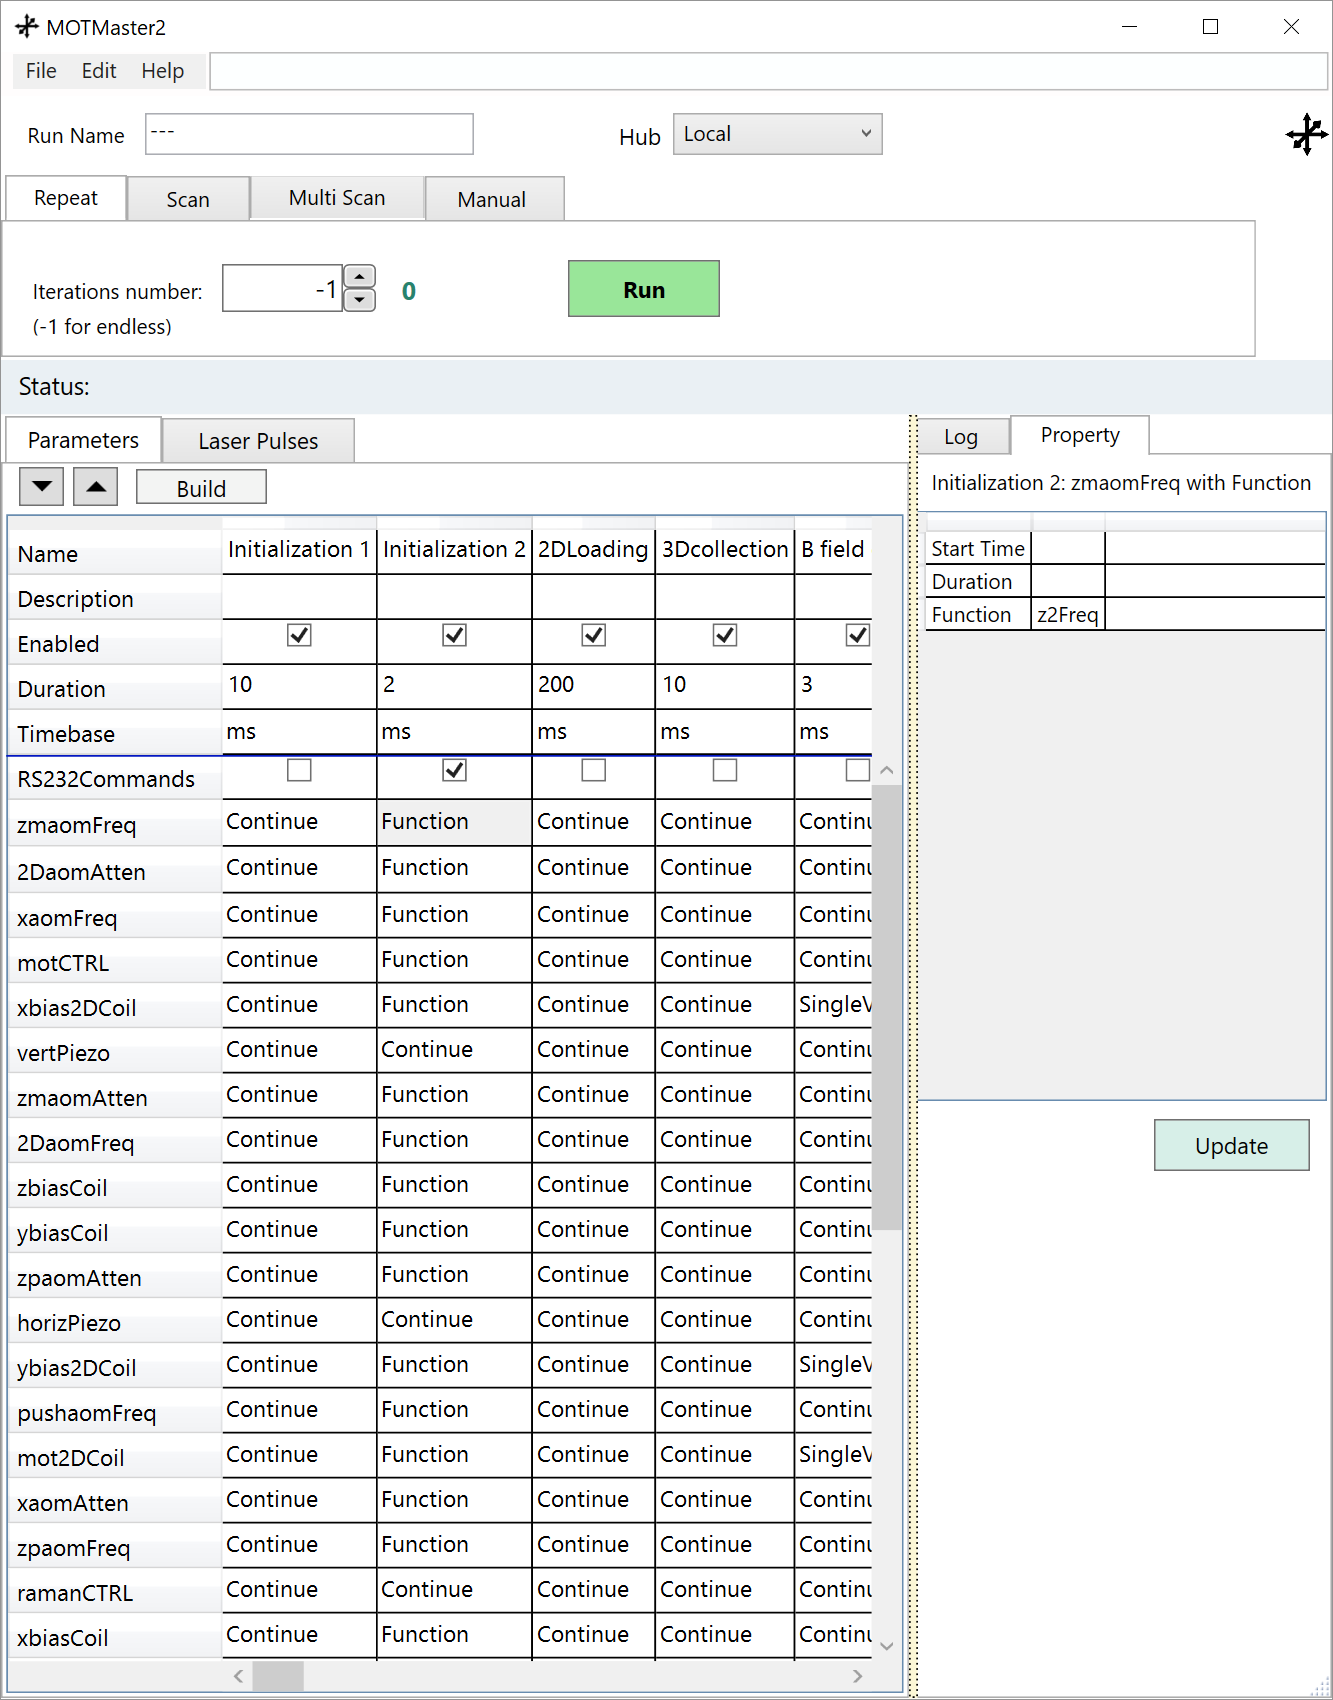
\includegraphics{motmaster_sequence.png}}
    \caption[MOTMaster user interface]{A sequence as represented in the MOTMaster user interface. Each step defines a duration and properties for each output channel. The sequence can either be run repeatedly, or configured to iterate through values of a chosen parameter.}
    \label{fig:motmaster_sequence}
\end{figure}
\par\noindent
After the sequence has finished, any acquired data from the analogue input channels is
streamed to the computer. The data per channel are segmented into arrays that
were acquired during each sequence step, before additional post-processing if
required. Finally, the hardware is reset to its initial state, before
starting the next experiment cycle.

\section{Experiment Control Hardware}\label{sec:mm_control_hardware}
In the preceding sections, the discussion of MOTMaster has been presented
without referring to specific hardware used in this experiment. Subsequent
chapters will introduce components of the experiment that are controlled by a
computer, but it is worth introducing the hardware used to implement this
control. A diagram of the control hardware is shown in~\FigureRef{fig:control_hardware}. All of the \ac{daq} cards are housed on a PXIe-1073 chassis, so that
timing signals such as start triggers and sample clocks can be shared on the
PXI backplane. The analogue output signals are generated on a
PXI-6723 card. This contains 32 analogue output channels and the output of
each is generated using a 13 bit \ac{dac}. Over the maximum voltage range of
\(\pm \sivalue{10}{\volt}\), this corresponds to an output quantisation of
\sivalue{2.44}{\milli\volt}, which did not limit the precision of any
analogue control in the experiment. The analogue output pattern is sampled at
a frequency of \sivalue{100}{\kilo\hertz}, which gives a minimum resolution
of \sivalue{10}{\micro\second}. Any jitter on this sample clock did not
produce any noticeable effects during the experiment. \par\noindent
Two cards on the chassis are able to acquire data from analogue inputs. The
first is a PXIe-6341, which has 16 input channels, each with a 16-bit
\ac{adc}. In addition to this, a counter channel on this card was used to trigger the output of serial messages. During the preliminary stages of the experiment, this bit-depth was
sufficiently large to prevent quantisation effects becoming significant. However
the AI-Q-2010 MEMS accelerometer used in the experiment, discussed further in \SectionRef{subsec:raman_mems}, has an equivalent voltage noise below this quantisation level. Therefore, a
PXI-4462 card, which contains 4 24-bit analogue input channels, was added.
This card is used to acquire data from devices where the higher voltage
resolution is desirable --- namely, the MEMS accelerometer and the
photodiode used to detect the population of atoms in each state after interference.\par\noindent
Digital output signals are generated using a PXI-6541 card. Unlike the
others, this card is controlled using the NI-HSDIO driver. With a maximum
sampling frequency of \sivalue{50}{\mega\hertz}, this card is capable of
generating digital signals at a much higher rate than the PXIe-6341, which
also contains digital output channels. However, the PXIe-6341 card only
contains 8 digital channels that can be timed using a hardware clock, fewer
than required to control the entire experiment.
\par\noindent
Two components of the experiment are controlled during the experiment using
serial communication. The first of these is an interface to the \ac{dds} on
the \Muquans\ laser which control the frequency of the cooling and repump
lasers and is controlled in real-time during the experiment. This
communication protocol is described in further detail in
\SectionRef{subsec:muquans_comm}. Finally, MOTMaster is configured to remotely connect to the M
Squared laser, so that it can control all the parameters necessary to drive
Raman transitions during the experiment. This is done by sending structured
JSON messages that contain commands to implement this control. More detail on how this is used in the experiment is given in
\SectionRef{subsuc:msquared_comm}.
\begin{figure}
    \centering
    \fontsize{16pt}{14pt}
    \resizebox{1\textwidth}{!}{\input{control_hardware.pdf_tex}}
    \caption[Control hardware schematic diagram]{Schematic diagram of the control hardware. The PXIe chassis contains the DAQ cards which generate the analogue and digital waveforms used to control other devices. Signals are routed between the cards to synchronise their operation. Serial communication to the \Muquans laser (\SectionRef{sec:muquans_light}), the M-Squared laser (\SectionRef{sec:msquared_laser})and the CCD camera (\SectionRef{sec:imaging}) are used for their control.}
    \label{fig:control_hardware}
\end{figure}

\section{Experimental Sequence Overview}
The experiment can be broken down into the following stages:
\begin{itemize}
    \item \underline{Loading}: Atoms are loaded from the 2D \ac{mot} into the 3D \ac{mot}.
    \item \underline{Molasses}: Atoms are released from the trap and cooled further in an optical molasses.
    \item \underline{State Preparation}: A sequence of optical and microwave pulses are used to prepare atoms with a narrow velocity spread in the \(\ket{1,0}\) state.
    \item \underline{Interferometry}: A \(\pi/2 - \pi - \pi/2\) sequence of laser pulses drive Raman transitions between the atoms.
    \item \underline{Dectection}: Two laser pulses are used to measure the number of atoms in \(\ket{F=2}\) and the total number, respectively. From these measurements, the interferometer phase difference can be inferred.
\end{itemize}

    \chapter{Laser Systems}\label{chap:setup}
This chapter provides a description of the hardware that makes up the experiment. Over the course of the project, the complexity of the experiment necessarily increased. The setup is presented in a bottom-up approach, starting from the most fundamental components, to provide a clear overview of the system. \\

\verysubsection{To-Do}
\begin{itemize}\item Figures describing each of the lasers
    \item Describe 3D and 2D MOT setups  
    \item Imaging systems
    \item Microwave synthesisers
    \item Raman Assembly
    \item MOT light distribution
\end{itemize}
\section{Chapter Overview}\label{sec:setup_overview}
The first two sections describe the two commercial laser systems used in this experiment. The \Muquans laser system which generates the light used for cooling and repump in the 2D and 3D \acp{mots}, referred to as the \acs{mot} light. The design and operation of this laser is given in \SectionRef{sec:setup_muquans}. A secondary laser system, built by MSquared, is used to generate light to drive Raman transitions between two hyperfine ground states in \ac{rb87}\footnote{The \Muquans laser also has a pair of lasers designed for driving Raman transitions, but these are not used in this experiment. \SectionRef{sec:setup_msquared} gives an explanation for this.}, otherwise referred to as Raman light. This is described in \SectionRef{sec:setup_msquared}.This is followed by a description of the vacuum chamber in \SectionRef{sec:setup_chamber} which contains both the 2D \ac{mot} (\SectionRef{subsec:setup_2DMOT}) and the 3D \ac{mot} (\SectionRef{subsec:setup_3DMOT}).  

\section{The \Muquans Laser System}\label{sec:setup_muquans}
\verysubsection{To-Do}
\begin{itemize}
    \item Laser Schematic
    \item Plots of lock signals
    \item DDS Serial communication
    \item Power output, stability
    \item Ref for error signal generation by current modulation
    \item Move some of this to appendix
\end{itemize}
All the \ac{mot} light in this experiment was generated by the \Muquans laser \cite{muquansWebPage}. \Muquans is a French laser company that is a spin-off from the Institut d'Optique and Observatoire de Paris. Consequently, their technology has been developed over a long history of performing experiments into atom interferometry using Rubidium. A schematic of this laser system is shown in \FigureRef{fig:muquans_schematic}. The \Muquans laser is comprised of four 1560nm \acp{ecdls} which are frequency-doubled to produce light at wavelengths close to 780nm. The telecommunications industry, which relies heavily on light in the 1530-1565nm wavelength band for optical communications, has motivated a rapid development in low-noise, robust lasers. In particular, this has enabled a design which does not require free-space optics and is much more resilient to effects such as temperature changes and vibrations, when compared to more conventional 780nm laser systems. The \Muquans laser contains one master laser \footnote{see \SectionRef{subsec:muquans_master} for more details}, which is locked to the \(F = 3 \rightarrow F' = 3,4\) crossover point in \ac{rb85}, and serves as an absolute frequency reference. The other three slave lasers are used for output. The first one is used to provide lightAll the \ac{mot} light in this experiment was generated by the \Muquans laser \cite{muquansWebPage}. \Muquans is a French laser company that is a spin-off from the Institut d'Optique and Observatoire de Paris. Consequently, their technology has been developed over a long history of performing experiments into atom interferometry using Rubidium. A schematic of this laser system is shown in \FigureRef{fig:muquans_schematic}. The \Muquans laser is comprised of four 1560nm \acp{ECDLs} which are frequency-doubled to produce light at wavelengths close to 780nm. The telecommunications industry, which relies heavily on light in the 1530-1565nm wavelength band for optical communications, has motivated a rapid development in low-noise, robust lasers. In particular, this has enabled a design which does not require free-space optics and is much more resilient to effects such as temperature changes and vibrations, when compared to more conventional 780nm laser systems. The \Muquans laser contains one master laser \footnote{see \SectionRef{subsec:muquans_master} for more details}, which is locked to the \(F = 3 \rightarrow F' = 3,4\) crossover point in \ac{rb85}, and serves as an absolute frequency reference. The other three slave lasers are used for output. The first one is used to provide light for cooling, as well as repump light by modulating the phase of this laser using an \ac{eom}. The other two make up a pair of lasers for driving Raman transitions. One laser is frequency-offset locked to the master and the other is phase-locked to the first, to ensure that the relative phase between the two lasers is constant. It should be noted that this Raman laser was not used in this experiment, so will not be discussed in great detail. Each of these slave lasers is amplified in an \ac{edfa} before being frequency doubled in a \ac{ppln} and passed through an \ac{aom} which is used to control the output power during the experiment.  for cooling, as well as repump light by modulating the phase of this laser using an \ac{eom}. The other two make up a pair of lasers for driving Raman transitions. One laser is frequency-offset locked to the master and the other is phase-locked to the first, to ensure that the relative phase between the two lasers is constant. It should be noted that this Raman laser was not used in this experiment, so will not be discussed in great detail. Each of these slave lasers is amplified in an \ac{edfa} before being frequency doubled in a \ac{ppln} and passed through an \ac{aom} which is used to control the output power during the experiment. 
\begin{figure}
    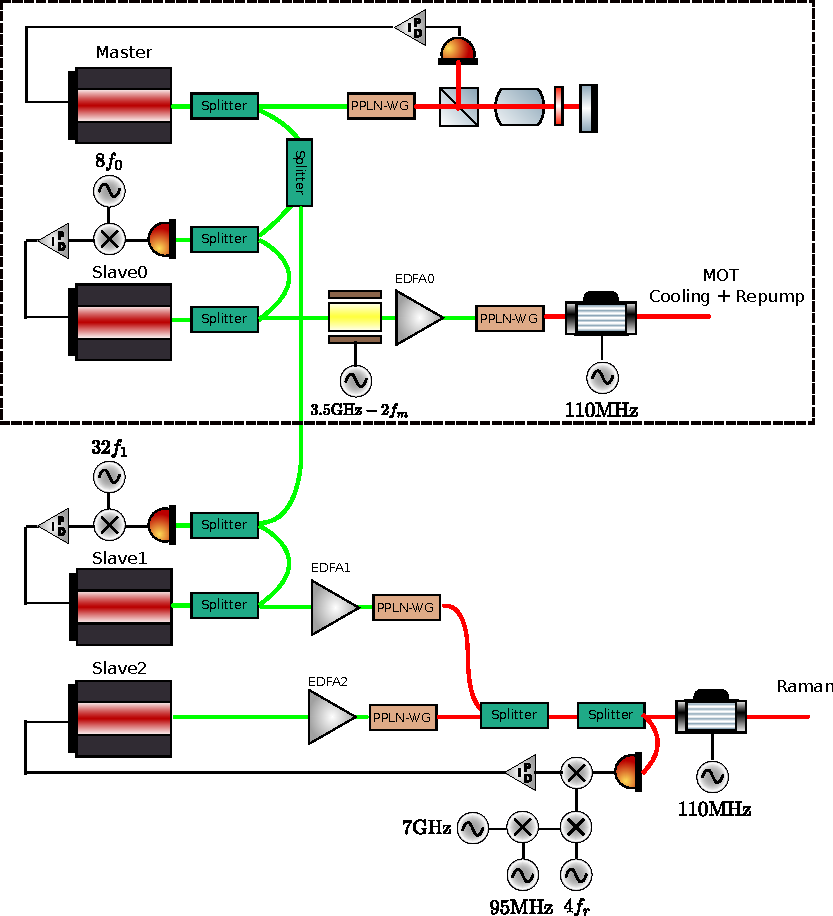
\includegraphics{muquans_schematic}
    \caption[\Muquans Laser System Diagram]{Schematic of the \Muquans laser system. Each output laser is derived from a 1560nm \acs{ecdl} (shown in green) which is amplified using an \acs{edfa} and then frequency-doubled to 780nm using a \acs{ppln} crystal. A master laser is locked to the 3,4 crossover in \ac{rb85} and the output lasers are offset-locked to their corresponding frequencies. The dashed region indicates the components used for generating light for the \acp{mots}, which was the only function of this laser for this experiment.}\label{fig:muquans_schematic}
\end{figure}
\subsection{Absolute Frequency Reference} \label{subsec:muquans_master}
The purpose of the master laser is to provide an absolute frequency reference so that the frequency of the output lasers can be controlled by comparing the difference frequency between them and the master. Lasers with linewidths narrower than their natural linewidth can be achieved by using a servo to stabilise their frequency and is essential for any experiment that requires laser light of a precise frequency. The frequency reference for the master is obtained using saturated absorption spectroscopy inside a Rubidium vapor cell. The sub-Doppler features in this spectrum are insensitive to temperature changes, and under sufficiently weak laser power have linewidths close to the natural linewidth of Rubidium (\(\Gamma \sim 2\pi \times 6\)MHz). \FigureRef{fig:muquans_satspec} shows the saturated absorption spectrum using the \Muquans master laser. This is obtained by fine adjustment of the temperature of the master \ac{ecdl}. The laser is set to lock to the crossover resonance between the \(F = 3 \rightarrow F' = 3\) and \(F = 3 \rightarrow F' =4 \) transitions in \ac{rb85} (indicated as \(b)\)), which is the strongest feature in the spectrum as well as being relatively close the the cooling transition in \ac{rb87} (indicated as \(a)\)).   
\begin{figure}
    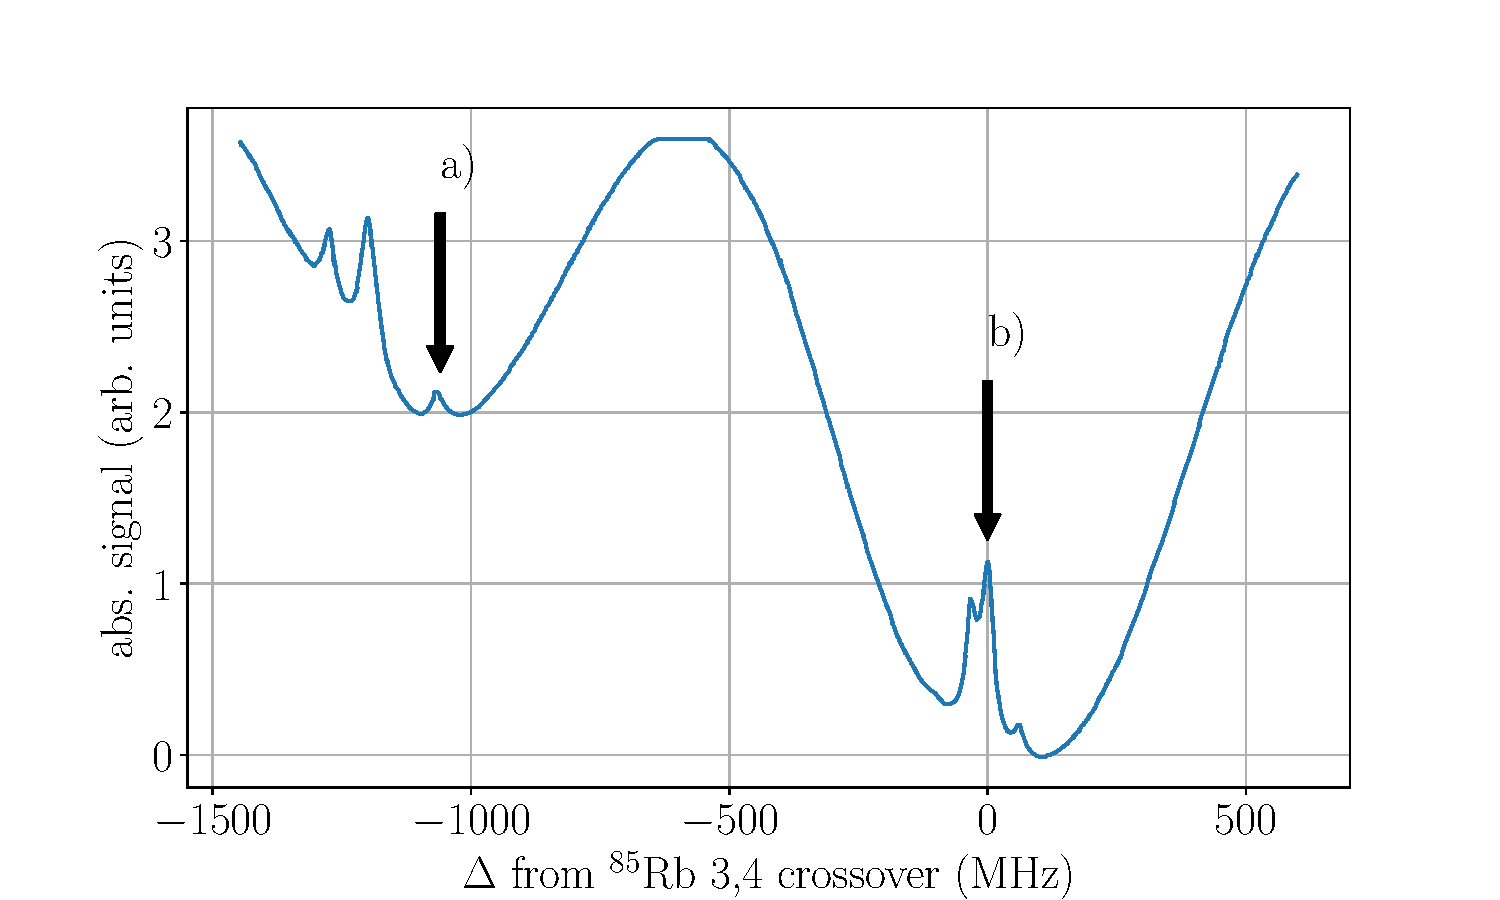
\includegraphics[width=0.6\textwidth]{sat_spec}
    \caption[Saturated absorption spectroscopy of the \Muquans master laser.]{Saturated absorption spectroscopy using the Rubidium vapour cell in the \Muquans laser. The absorption features indicated are \(a)\): the \(F = 2 \rightarrow F' = 3\) transition in \ac{rb87} and \(b)\): the crossover resonance between the \(F = 3 \rightarrow F' = 3\) and \(F = 3 \rightarrow F' =4 \) transitions in \ac{rb85} which is used to lock the frequency of the master laser.}
    \label{fig:muquans_satspec}
\end{figure}
\begin{figure}
    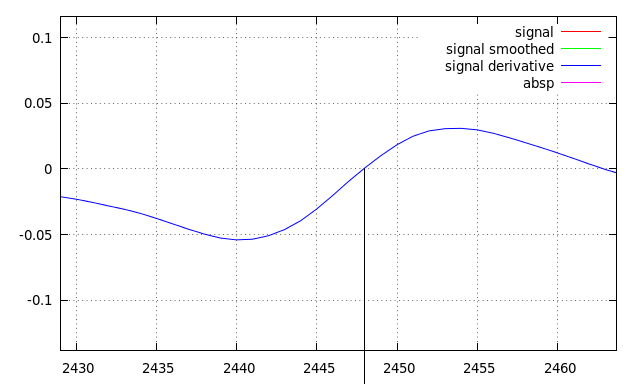
\includegraphics[width=0.6\textwidth]{error_signal}
    \caption[Error Signal for the \Muquans master servo.]{Error signal obtained by modulating the laser current. Close to the lock point, the signal is approximately linear. This signal is used in a feed-back loop to correct for frequency changes of the master laser.}
    \label{fig:muquans:error_signal}
\end{figure}
Some form of feed-back onto the master laser is required to keep its frequency fixed. The simplest way to achieve this is to use a signal that is linearly proportional to the deviation in frequency from the set-point, if one exists. The frequency of the laser is modulated by weakly modulating the current to the master \ac{ecdl}. {\textbf add more detail about the error signal lineshape} The error signal shown in \FigureRef{fig:muquans_errorsignal} is obtained by demodulating the absorption signal using a lock-in amplifier. In fact, this current modulation is always present on the master laser and the saturated absorption spectrum shown previously has been processed to average out the effects from this fast frequency modulation. In addition to proportional feed-back from the error signal, the servo that controls the master frequency also contains an integrator to compensate for long-term drifts. Typically, these arise from external temperature changes and if unaccounted for, they could cause the laser to unlock. In the conditions of our laboratory, where the temperature is externally controlled, this has never occurred.  
\subsection{Generating MOT light}
\subsection{Raman light}
\subsection{Real-time Frequency Control}
\section{The M-Squared Laser System}\label{sec:setup_msquared}
\verysubsection{To-Do}
\begin{itemize}
    \item Schematic
    \item Raman PLL phase-noise
    \item Laser Control
    \item DCS module
\end{itemize}
\subsection{Laser Specifications}
\subsection{The DCS Control Module}
\subsection{Frequency Control of the Raman Lasers}
\subsection{Controlling the Phase Difference}

    %\chapter{Cooling and Trapping in a MOT}\label{chap:mot}
\section{Chapter Overview}
This chapter presents a description of the components of the experiment which
are used to trap and cool atoms in a \ac{mot}. An outline of the hardware used
to create both the 2D and 3D \acp{mots} is presented
o
in~\SectionRef{sec:vacuum_chamber}. Following this is a description of the
\Muquans laser system, in~\SectionRef{sec:muquans_light}, which generates the
light used to cool and trap atoms. The hardware used to control the frequency
and power of each \ac{mot} beam, as well as the required magnetic fields, is
given in~\SectionRef{sec:mot_control}. Finally, this chapter concludes with a
characterisation of the 3D \ac{mot} loading rate in~\SectionRef{sec:mot_characterisation}
\section{The Navigator Vacuum Chamber}\label{sec:vacuum_chamber}
The vacuum chamber, along with the components mounted to it, make up the
majority of the hardware used in the preliminary trapping and cooling
stages of
the experiment. \FigureRef{fig:mot_system} shows a diagram of the
vacuum chamber and the main \ac{mot} components. The chamber is made of 316L stainless
steel, which has a low magnetic permeability to reduce stray magnetic
fields on the atoms. It contains 16 DN40
ConFlat ports arranged
on the edges of three octagons, one in each Cartesian coordinate plane. Six of
these ports provide optical access for the 3D \ac{mot}. Another port
connects the 2D \ac{mot} system to the main chamber. One port provides
optical access for either a CCD camera or photodiode. Opposite this is
a microwave horn for driving microwave transitions between the two
\ac{rb87} hyperfine ground states. The remaining ports are not
used for optical access since
they do not have a direct line of sight to the atoms. Instead, these
are used to mount a pressure gauge, gate valve, a \ac{neg} pump
and electrical feedthroughs for the \ac{mot} coils. 
\par\noindent
Two oppositely-facing DN63
ports are used to mount the optics for driving Raman transitions\footnote{For more information about the Raman optical system,
refer to \ChapterRef{chap:raman_optics}}. This is the axis along which the atom interferometer is sensitive to
accelerations, subsequently referred to as the Raman axis.
\par\noindent  The chamber is pumped down to a pressure of around
\pow{5}{-10}\sivalue{}{\milli\bar} using a NexTorr D100-5 pump. This is a
composite system consisting of \ac{neg} and an ion pump. The \ac{neg} is a
porous sintered zirconium (St 172) element, which reacts with chemicals such as
hydrogen, water, nitrogen, oxygen and hydrocarbons. Most of these were removed
during the initial baking and roughing pump stages. Under \ac{uhv} conditions,
the largest contributor to the pressure is hydrogen which the \ac{neg} can pump
at a speed of \sivalue{100}{\litre\per\second}. Any species that are not
absorbed by the \ac{neg}, in particular Rubidium, are pumped by the
\sivalue{5}{\litre\per\second} ion pump.
\begin{figure}[!htbp]
	\centering
	\def\svgwidth{1\textwidth}
	\input{Figures/Chapter4/Vacuum.pdf_tex}
	\caption[\ac{mot} system component diagram]{A diagram of the main components on the vacuum chamber used for the \ac{mot}
		systems. Rubidium atoms are dispensed and loaded into the 2D \ac{mot}
		before being pushed into the main chamber and collected in the 3D
		\ac{mot}. A set of 6 beam collimators provide the light to
		slow and cool atoms.  A spherical quadrupole
		field traps atoms at the centre of the chamber. Not shown are additional bias
		coils along each \ac{mot} beam axis to null stray fields at the centre
		of the chamber.}
	\label{fig:mot_system}
\end{figure}
\subsection{The 2D MOT system}\label{sec:2d_mot}
At room temperature, a large fraction of atoms have velocities greater than typical \ac{mot} capture velocities, so a very high partial pressure of
Rubidium is needed to achieve a fast loading rate from a background
vapour. This also contributes to a high background atom number, which
reduces the interferometer fringe visibility. Loading from a 2D
\ac{mot} system both increases the loading rate
and decreases the pressure inside the main chamber~\cite{Dieckmann1998}.  \par\noindent A diagram of the light and magnetic fields
required to produce a 2D \ac{mot} is presented
in~\FigureRef{fig:2D_mot_diagram}. It is similar to the 3D \ac{mot}, with the
main exception being that only 4 beams are used to cool the atoms along 2
orthogonal axes. It is designed to produce a large flux of cold atoms which can be subsequently loaded into a
3D \ac{mot}~\cite{Muller2007,Roos2003}. The cooling beams are collimated to a
large waist size and the magnetic field coils produce a cylindrical quadrupole
field with a line of zero magnetic field along the axis of symmetry. Along this
axis, the atoms are free to move, resulting in an atomic beam. This
beam is collimated using a larger radial field gradient than is
typically found in 3D \ac{mot} systems. This increases the radial
confinement of
atoms. 
\par\noindent 
A pinhole is placed at the exit of the cell to prevent atoms with
with a high radial velocity from exiting. This pinhole also
greatly reduces the conductance between the 2D \ac{mot} cell and the main
chamber, which means that a high rubidium partial pressure can be maintained in the 2D \ac{mot} cell, without greatly
increasing the pressure in the main chamber. The pinhole is drilled into a
silicon plate, which partially reflects the beam that propagates along
the central axis. This creates an unbalanced molasses that cools atoms
along the axial direction. The scattering rate from each beam is not
equal, so the net force on the atoms pushes them through the pinhole.
By slowing a larger proportion of atoms to within the
capture velocity of the 3D \ac{mot}, this configuration, referred to as a 2D\(+\)
\ac{mot}, loads a 3D \ac{mot} faster than the 4-beam counterpart. \par\noindent
\begin{figure}[!htbp]
	\centering
	\def\svgwidth{0.5\textwidth}
	\input{Figures/Chapter4/2D_mot.pdf_tex}
	\caption[Schematic for the 2D \ac{mot}]{Schematic diagram for the 2D \ac{mot}. \ac{rb87} atoms are trapped and cooled along the 2 axes orthogonal to the long axis of the source cell. The black arrows indicate the direction of the current through each coil. Each circularly polarised beam drives \(\sigma^-\) transitions for an atom moving in the opposite direction. A linearly polarised push beam propagates along the longitudinal axis and is partially reflected by the silicon wafer at the opposite end. This provides a small amount of axial cooling and the imbalance of radiation pressure pushes atoms out of the cell. The pinhole at the other end prevents atoms with a high transverse velocity from leaving the cell.}
	\label{fig:2D_mot_diagram}
\end{figure}
\FigureRef{fig:2D_mot_optics} shows a schematic of the optical
components used to generate the light for the 2D \ac{mot}. The cooling
light enters from a single
fibre, which is collimated to a beam waist of
\sivalue{9.5}{\milli\metre} using two aspheric lenses. This is
linearly polarised and divided
into two beams of equal power using a \ac{hwp}, one for each cooling
axis. Each beam passes
through a beam-splitter and a prism mirror, to increase the volume
covered by
the 2D \ac{mot} beams. A \ac{qwp} circularly polarises the beam before
it enters the ar-coated glass cell. On the opposing side of the cell, a
\(\sivalue{25}{\milli\metre} \times \sivalue{35}{\milli\metre}\) mirror retro-reflects the beam. This is coated with a layer of quartz to form a \ac{qwp}, so that the
reflected beam has the same polarisation handedness as the incoming.
\par\noindent 
The push beam enters from a second fibre input. A fixed focus collimator collimates
the beam to a waist of \sivalue{1.5}{\milli\metre}. This is mounted onto a
\sivalue{1}{\inch} kinematic mount to align the push beam to the \sivalue{0.7}{\milli\metre} pinhole at the other end of the cell. The push beam is linearly polarised by a \ac{pbs} to reduce the effect of
polarisation drift on the axial cooling of the 2D \ac{mot}. 
\par\noindent
The cell,
manufactured by ColdQuanta, has dimensions of \(\sivalue{30}{\milli\metre}
\times \sivalue{30}{\milli\metre} \times \sivalue{44}{\milli\metre}\) and is
specifically designed for creating a 2D\(+\) \ac{mot}. It contains two rubidium
dispensers composed of rubidium chromate (RbCrO\(_4\)) and a reducing agent.
These were activated by passing a large current through them to remove a thin
oxidation layer. To produce rubidium, a current of around \sivalue{2.8}{\ampere} is passed through the dispenser
to trigger an electro-chemical reduction reaction, so that pure rubidium sublimates.
\begin{figure}[!htbp]
	\centering
	\def\svgwidth{0.7\textwidth}
	\input{Figures/Chapter4/2D_mot_optics.pdf_tex}
	\caption[Optical components for the 2D \ac{mot}]{Optical components for the 2D \ac{mot}. The light for the \ac{mot} is split into two equal portions using a \ac{hwp} and \ac{pbs}. Along each axis, the beam passes through a \ac{pbs} and a prism mirror to increase its spatial extent. The beam is circularly polarised before entering the cell and retro-reflected by a mirror coated with a \ac{qwp}. The push beam is collimated from another fibre input and linearly polarised before entering the cell along the longitudinal axis.}
	\label{fig:2D_mot_optics}
\end{figure}
\par\noindent The cylindrical quadrupole field is generated by a set of coils
that are manufactured by ColdQuanta. They are mounted so that the axis of
zero magnetic field coincides with the central longitudinal axis of the source
cell. These produce a radial field gradient per current of
\sivalue{20}{\gauss\per\centi\metre\per\ampere}.
\FigureRef{fig:2d_mot_field_gradient} shows a simulation of the field
gradient along each axis and the magnetic field in each plane of
symmetry. 
Across the centre of the cell, the field gradient is very uniform. The
equilibrium position where the \ac{mot} forms is adjusted using
Helmholtz coil pairs along each \ac{mot} axis. These coils produce a
field per current of
\sivalue{1}{\gauss\per\ampere}.
\begin{figure}[!htbp]
	\centering
	\def\svgwidth{\columnwidth}
	\subfloat[][]{\scalebox{0.3}{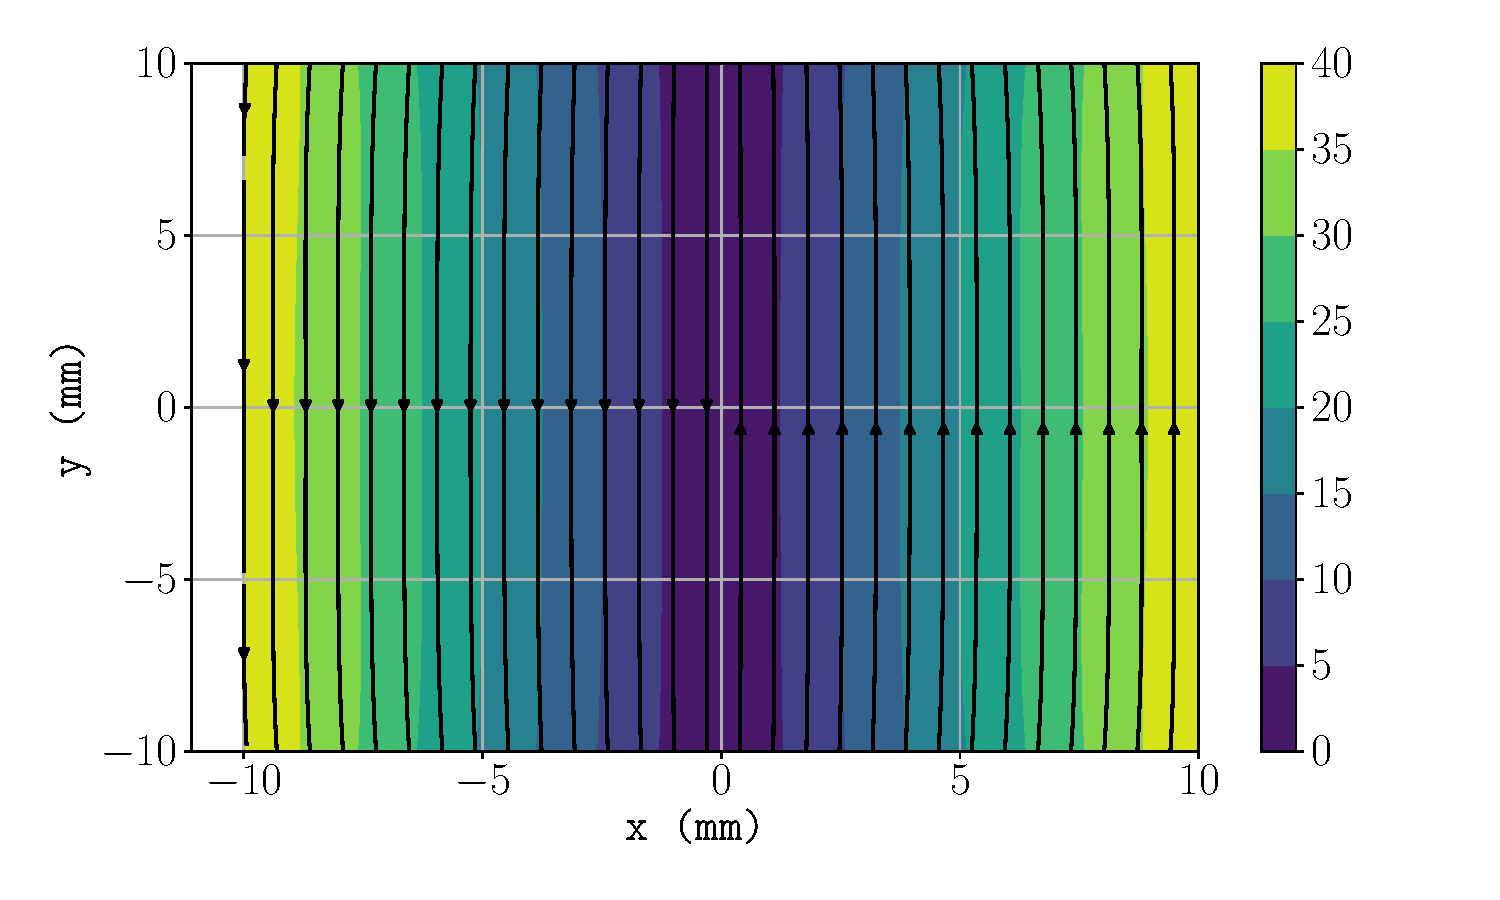
\includegraphics{2D_field_xy.pdf}\label{fig:2d_field_xy}}}
	\subfloat[][]{\scalebox{0.3}{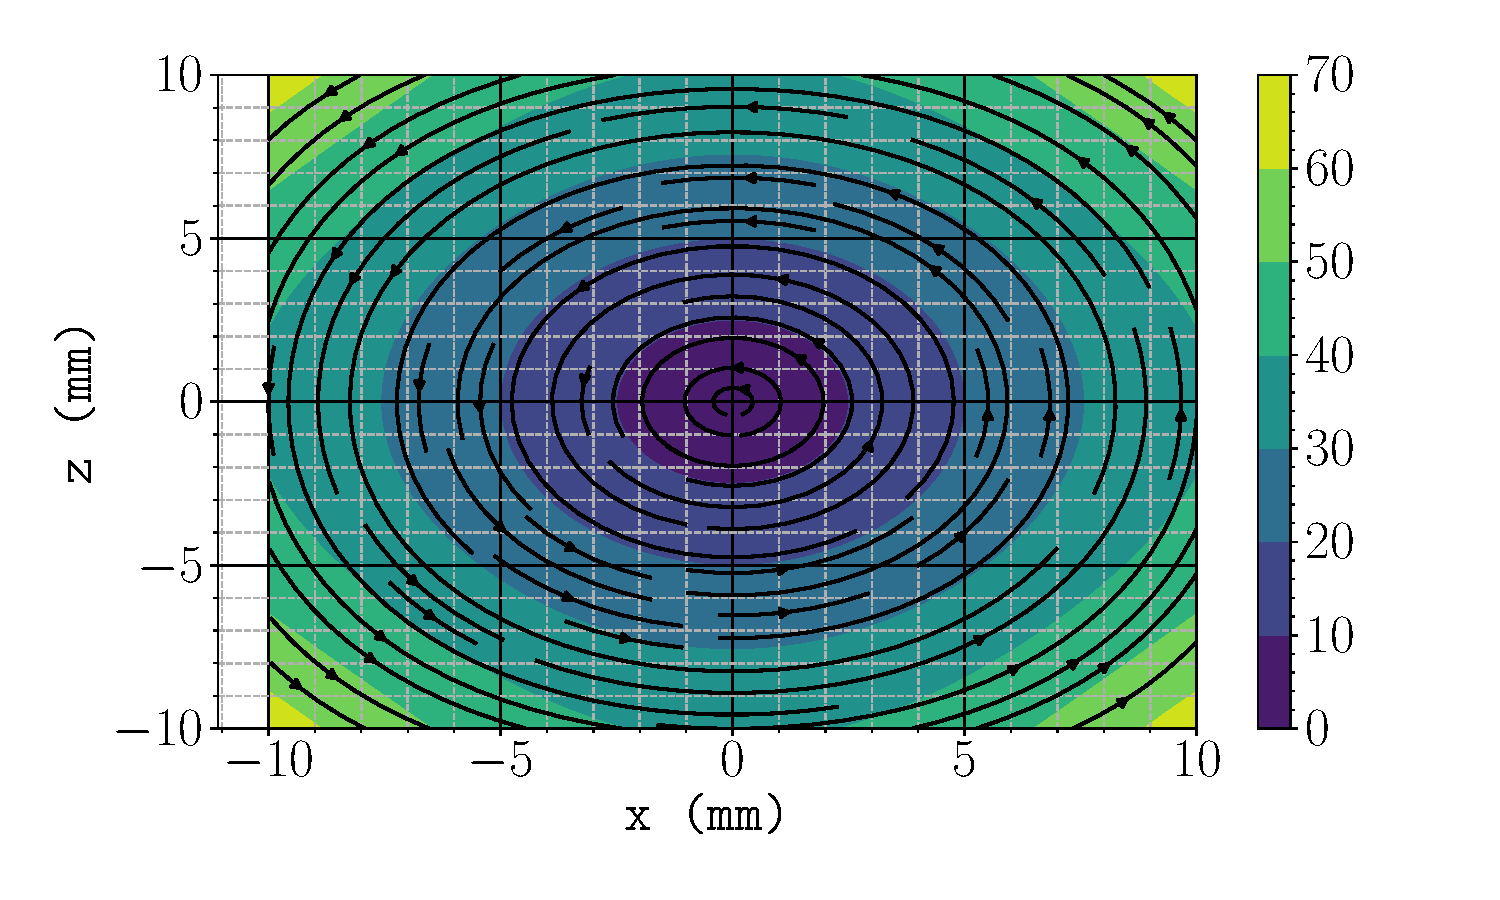
\includegraphics{2D_field_xz.pdf}}\label{fig:2d_field_xz}}\\
  \subfloat[][]{\scalebox{0.3}{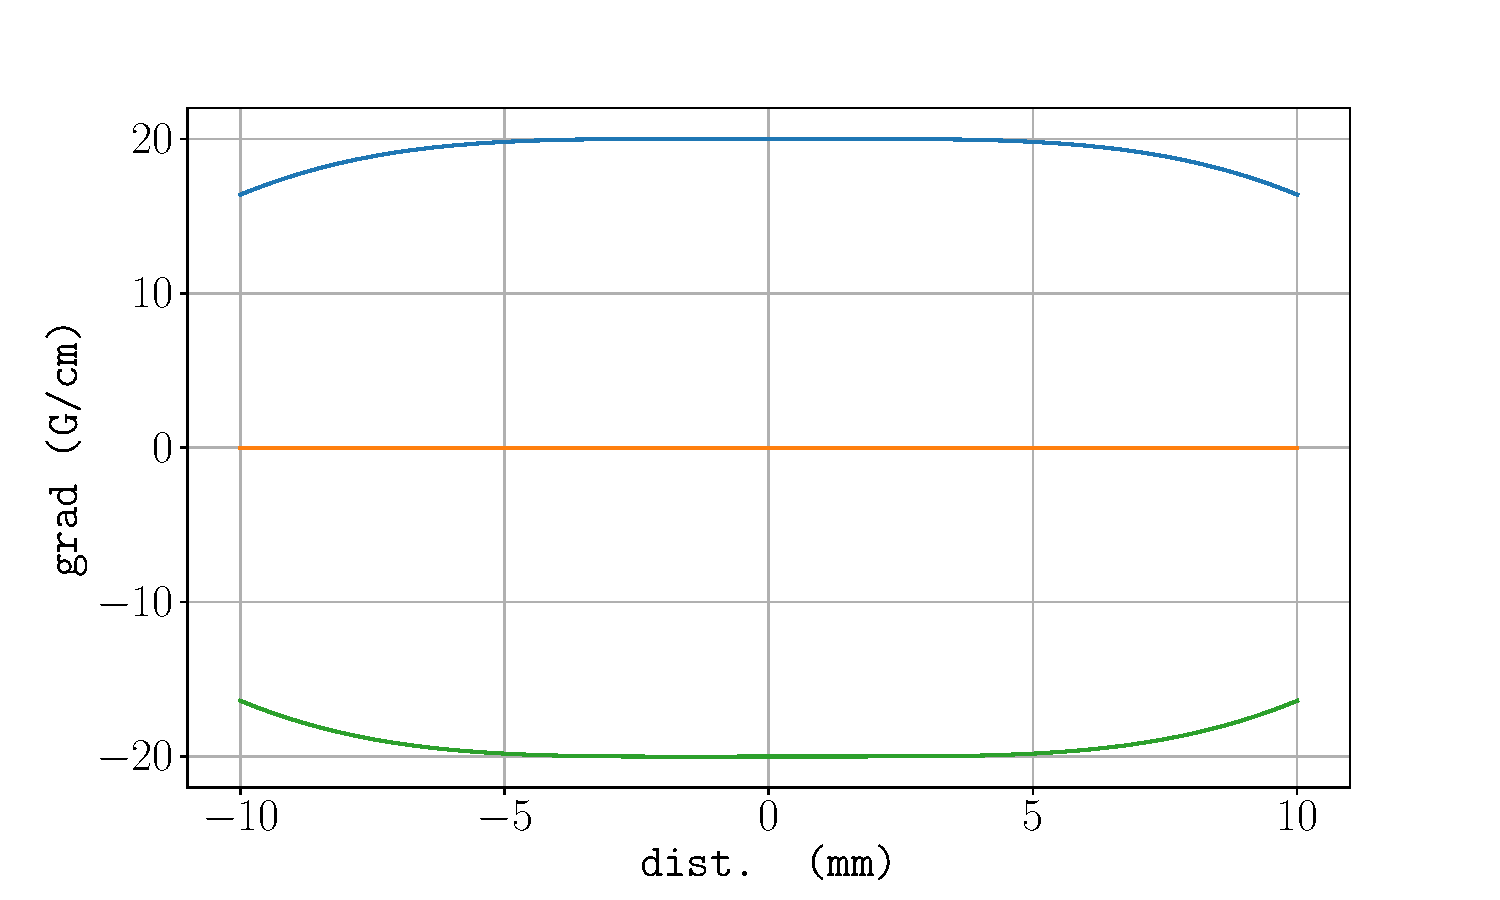
\includegraphics{2D_grad.pdf}}\label{fig:2d_grad}}
	\caption[Simulated field and field gradients for the 2D \ac{mot} quadrupole
		coils]{Simulated field and field gradients for the 2D \ac{mot}
		quadrupole coils. In this coordinate system, the 2D \ac{mot}cools and
		traps atoms in the \(\vec{x}\) and \(\vec{z}\) directions. The
		simulation was performed using a nominal current of
		\sivalue{1}{\ampere}, which corresponds to a current density in each
		coil of \sivalue{7.78}{\ampere\per\square\milli\metre}. The magnitude of
		the magnetic field (in units of \sivalue{}{\gauss}) and its direction in
		the axial and radial planes of symmetry are shown in \textbf{(a)} and
		\textbf{(b)}, respectively. \textbf{(c)} shows the field gradient
		components \(\partial_x B_x\) (blue), \(\partial_y B_y\) (orange) and
		\(\partial_z B_z\) (green) along their corresponding axes.}
	\label{fig:2d_mot_field_gradient}
\end{figure}
\subsection{The 3D MOT system}\label{sec:3d_mot}
The main chamber contains the apparatus that is used to make a 3D
\ac{mot}~\cite{Raab1987}. Each \ac{mot} beam originates from a \ac{pm} fibre and is collimated using a
lens with a nominal focal length of \sivalue{75}{\milli\metre} to a waist size of \sivalue{7.5}{\milli\metre}. At the output
of each collimator is a \ac{qwp}, with its slow axis oriented at a 45\(^\circ\)
angle to either the fast or slow axis of the fibre, to produce either left- or right-handed circularly polarised light. The \ac{mot} beams along the axial direction of the quadrupole field
(i.e. the \(\vec{z}\) direction) are orthogonally
polarised to the others along the \(\vec{x}\) and \(\vec{y}\) directions. The \ac{mot} beams are aligned so that their intensities at the centre of the chamber are equal, so that the \ac{mot} forms where the magnetic field is zero.
\subsubsection{Spherical quadrupole magnetic field}
The magnetic field for the 3D \ac{mot} is created by a pair of coils in an
anti-Helmholtz configuration. Each coil is wound using rectangular wire coated in a
\sivalue{35}{\micro\metre} thick layer of Pyre-M.L, a UHV-compatible polyamide
which provides a layer of insulation between each loop. The wire has a
cross-section of dimensions \(\sivalue{1.1}{\milli\metre} \times
\sivalue{1.1}{\milli\metre}\), with 20 axial loops and 12 radial loops. The
inner diameter of the coil is \sivalue{25.4}{\milli\metre}, to allow for optical
access of the \(\vec{z}\)-axis \ac{mot} beams, and the maximum diameter is
\sivalue{59.2}{\milli\metre} -- small enough that the coil could be
inserted into the chamber through the DN63 CF ports. The coils are mounted to
the chamber using groove grabbers which clamp into grooves inside the wall of
the DN40 ports. The coil formers increase the surface area in contact
with the chamber, increasing the rate of heat dissipation from the
coils. 
\par\noindent 
\FigureRef{fig:mot_coil_temp_both}~shows the temperature rise during
operation of the coils both at atmospheric pressure and inside the chamber. At a pressure of around  \sivalue{1e-2}{\milli\bar}, the temperature of the coils inside the chamber does not exceed \sivalue{40}{\celsius}. Once mounted, the distance between the innermost
loops is \sivalue{70}{\milli\metre}. \FigureRef{fig:coil_a} shows the
magnetic field, measured using a Hall probe, along the axis of symmetry for each
of the coils with a current of \sivalue{2.53}{\ampere}.
\FigureRef{fig:coil_b} shows the axial field measured when the coils are in anti-Helmholtz configuration. These are in close
agreement with a simulation of the magnetic field. The simulated field in the axial and radial planes of symmetry are shown
in~\FigureRef{fig:3D_mot_axial} and~\FigureRef{fig:3D_mot_radial}, respectively.
\begin{figure}[!htbp]
	\centering
	\def\svgwidth{\columnwidth}
	\subfloat[][]{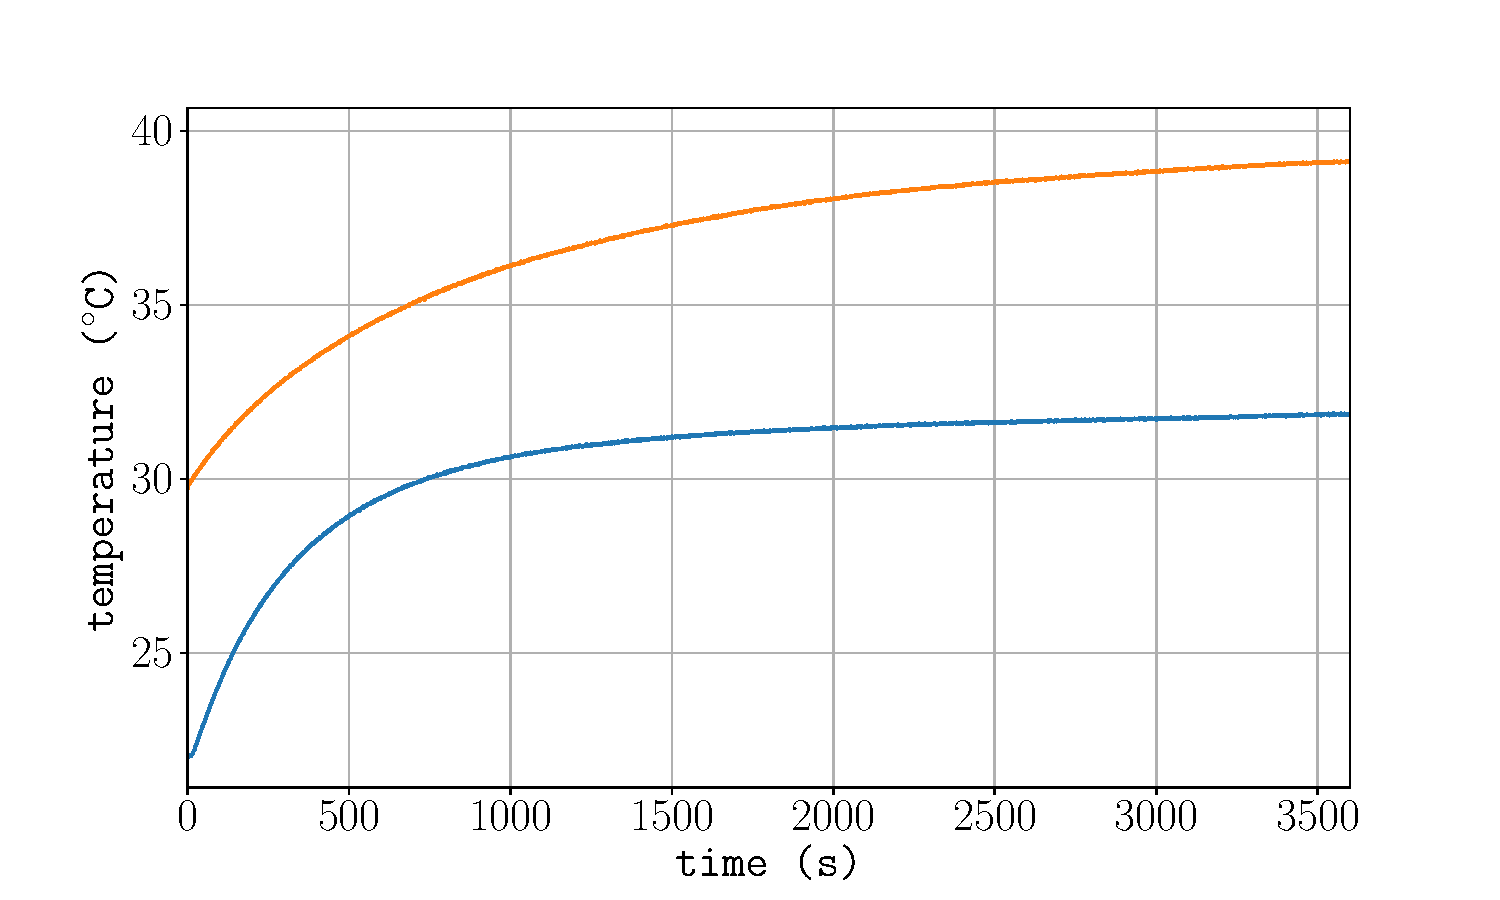
\includegraphics[width=0.45\textwidth]{mot_coil_temperature.pdf}}\label{fig:mot_coil_temp}
	\subfloat[][]{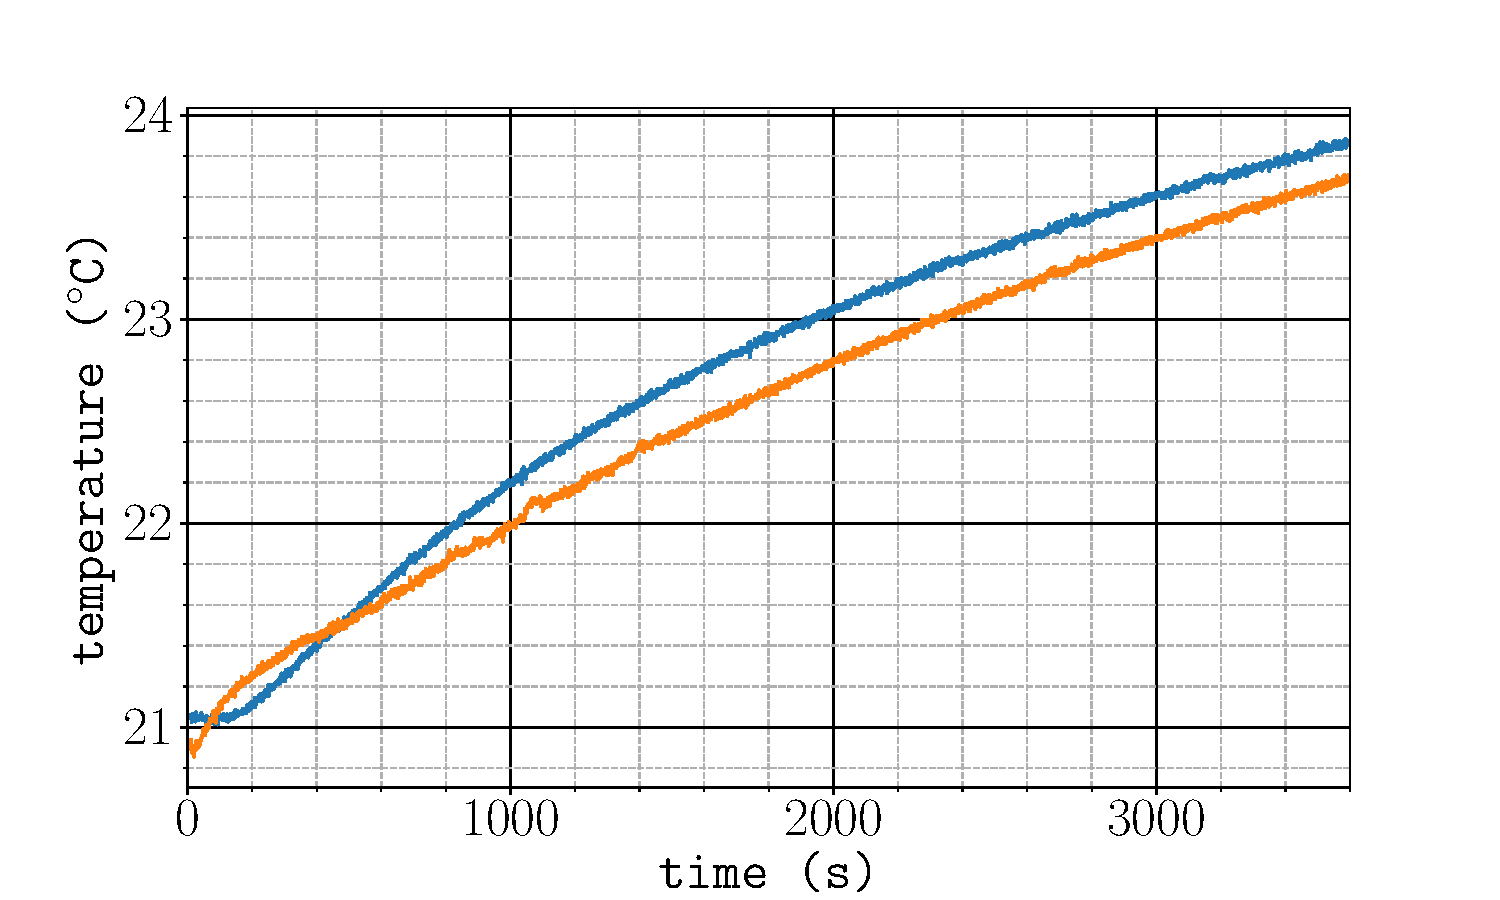
\includegraphics[width=0.45\textwidth]{mot_coil_temperature_chamber.pdf}}\label{fig:mot_coil_temp_tg4}
	\caption[\ac{mot} coil temperature rise]{Temperature rise due to the \ac{mot} coils over 1 hour of operation. The blue curves were measured when the coils were at atmosphere and the orange were measured under a rough vacuum around \sivalue{1e-2}{\milli\bar}. \textbf{(a)} shows the temperature of the coils and \textbf{(b)} is the temperature of the exterior of the chamber.}
	\label{fig:mot_coil_temp_both}
\end{figure}

\begin{figure}[!htbp]
	\centering
	\def\svgwidth{\columnwidth}
  \subfloat[][]{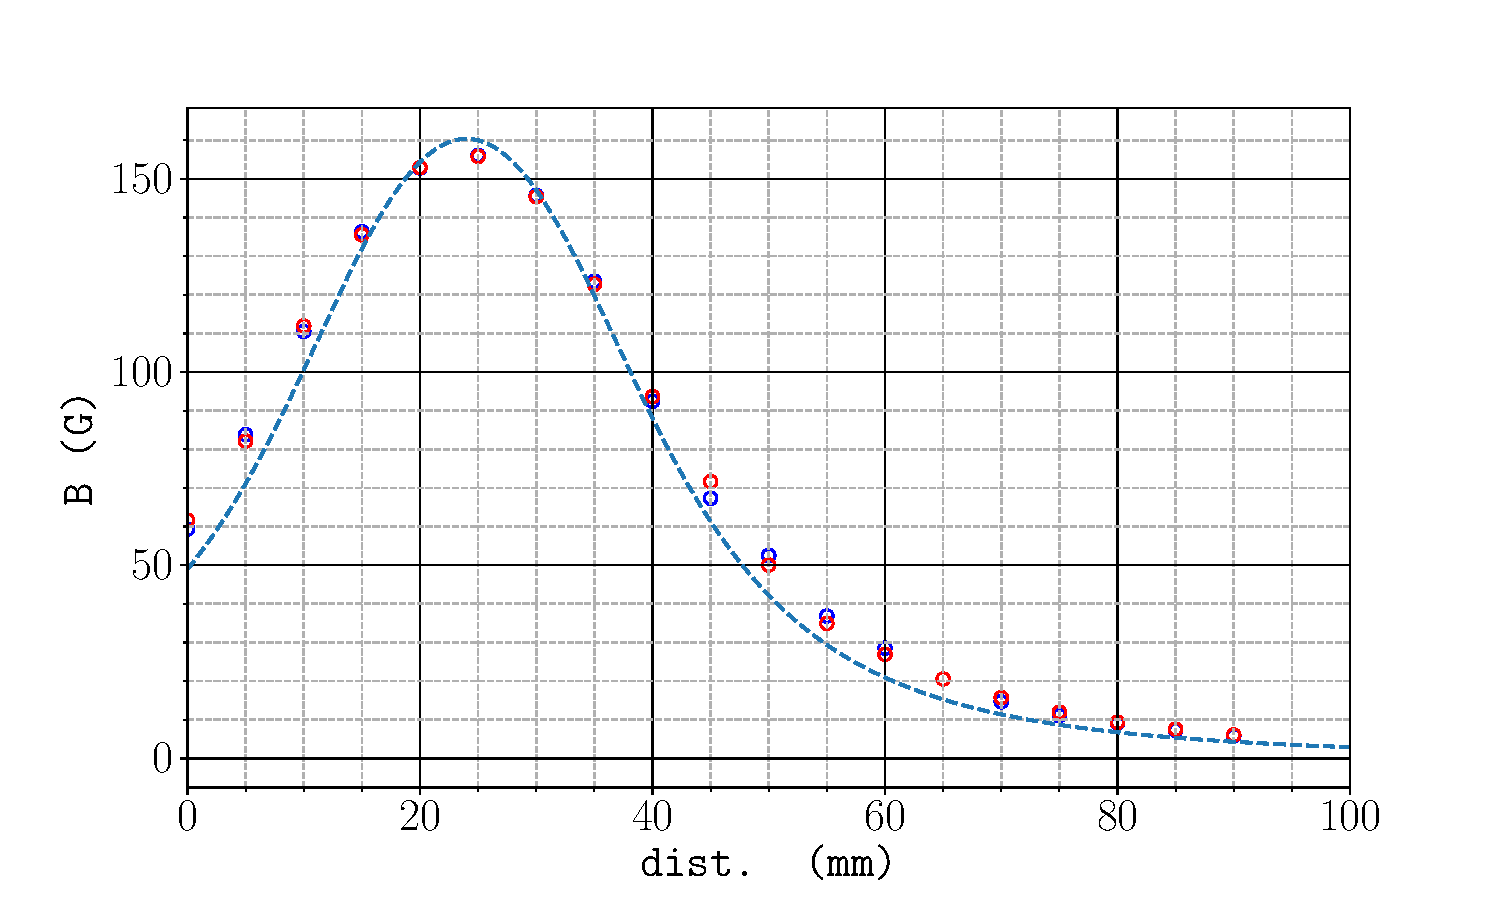
\includegraphics[width=0.45\textwidth]{mot_field_3D.pdf}}\label{fig:coil_a}
  \subfloat[][]{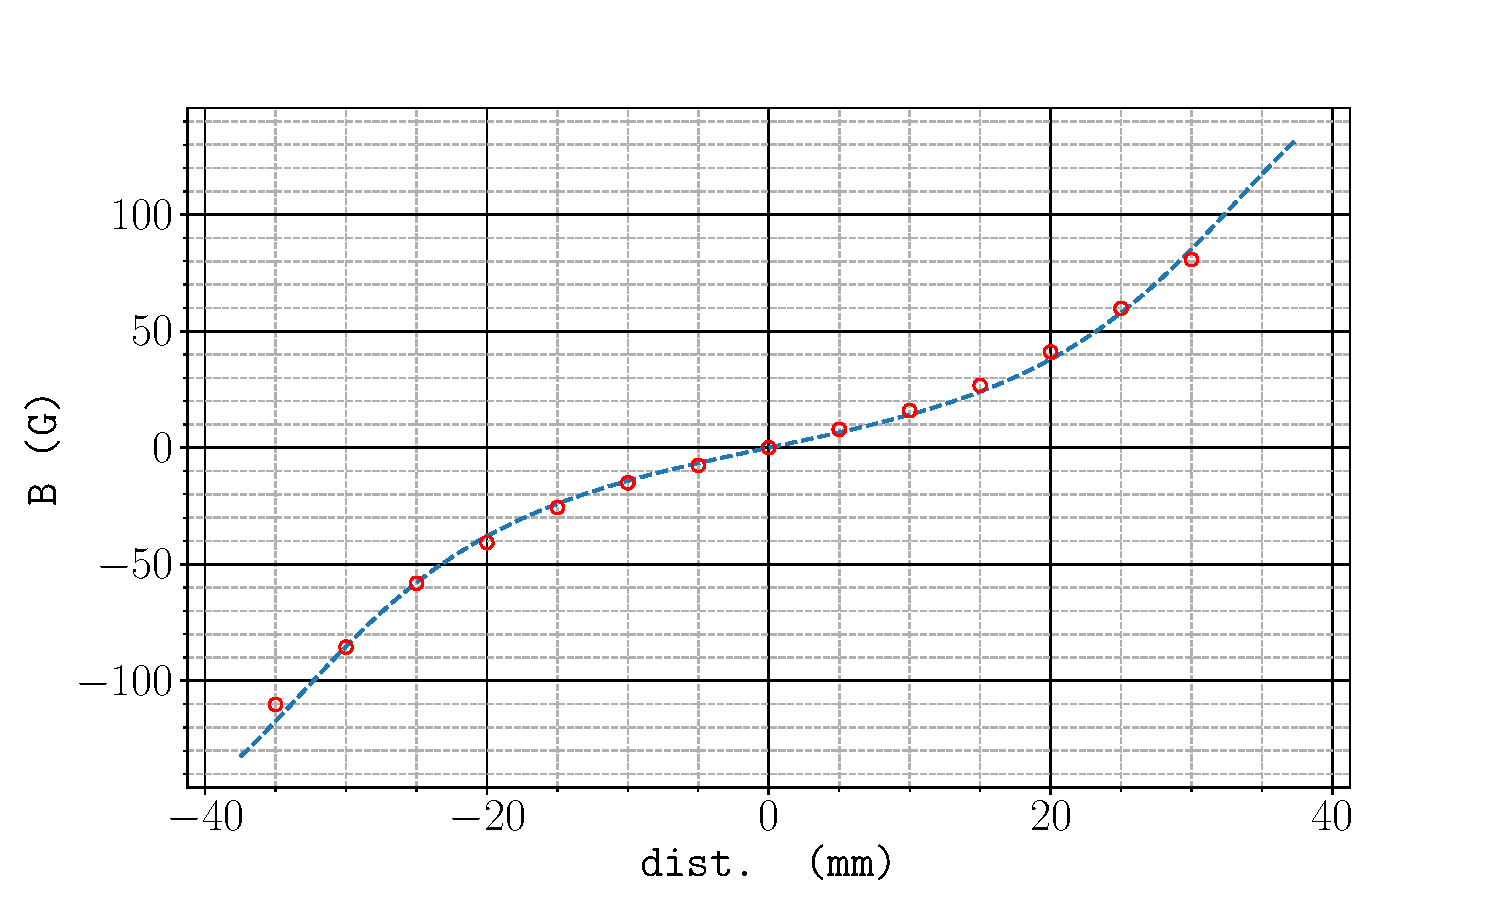
\includegraphics[width=0.45\textwidth]{mot_field_together_3D.pdf}}\label{fig:coil_b}
	\caption[Measured magnetic field and field gradient for the 3D \ac{mot}
		coils]{Measured magnetic field and field gradient for the 3D \ac{mot}
		coils. \textbf{(a)} shows the axial magnetic field for the two coils as
		measured using a Hall probe. \textbf{(b)} shows the field close to the centre when the coils are in an anti-Helmholtz configuration. The dashed lines indicate the axial field as
		calculated from the simulation shown
		in~\FigureRef{fig:3D_mot_field_sim}.}
    \label{fig:mot_coil_plots_subfig}	
\end{figure}

\begin{figure}[!htbp]
	\centering
	\def\svgwidth{\columnwidth}
	\subfloat[][]{\scalebox{0.3}{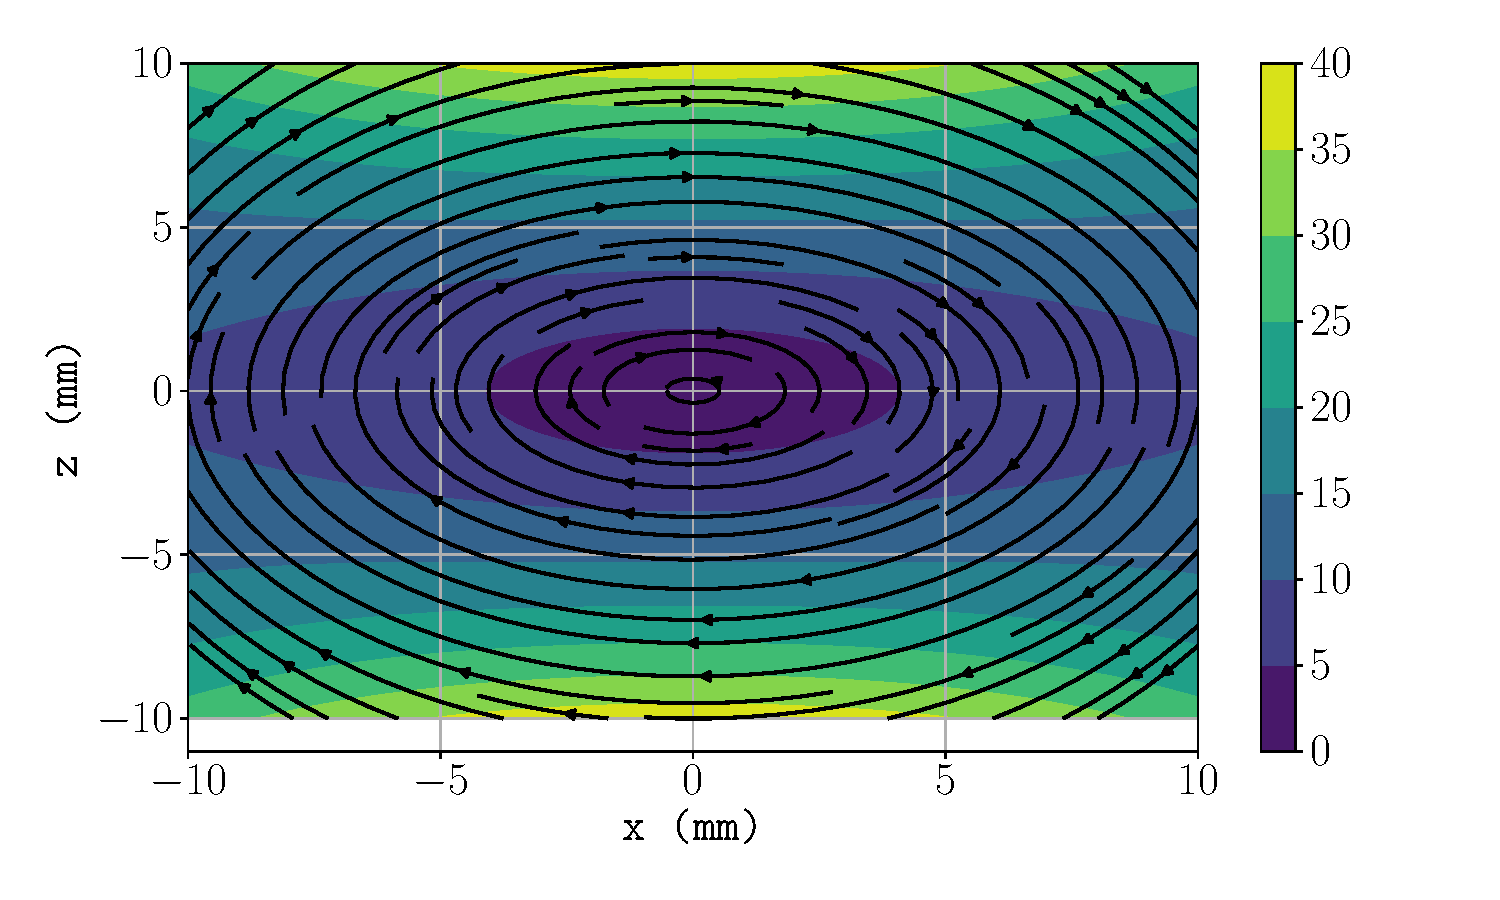
\includegraphics{3D_field_xz.pdf}}\label{fig:3D_mot_axial}}
	\subfloat[][]{\scalebox{0.3}{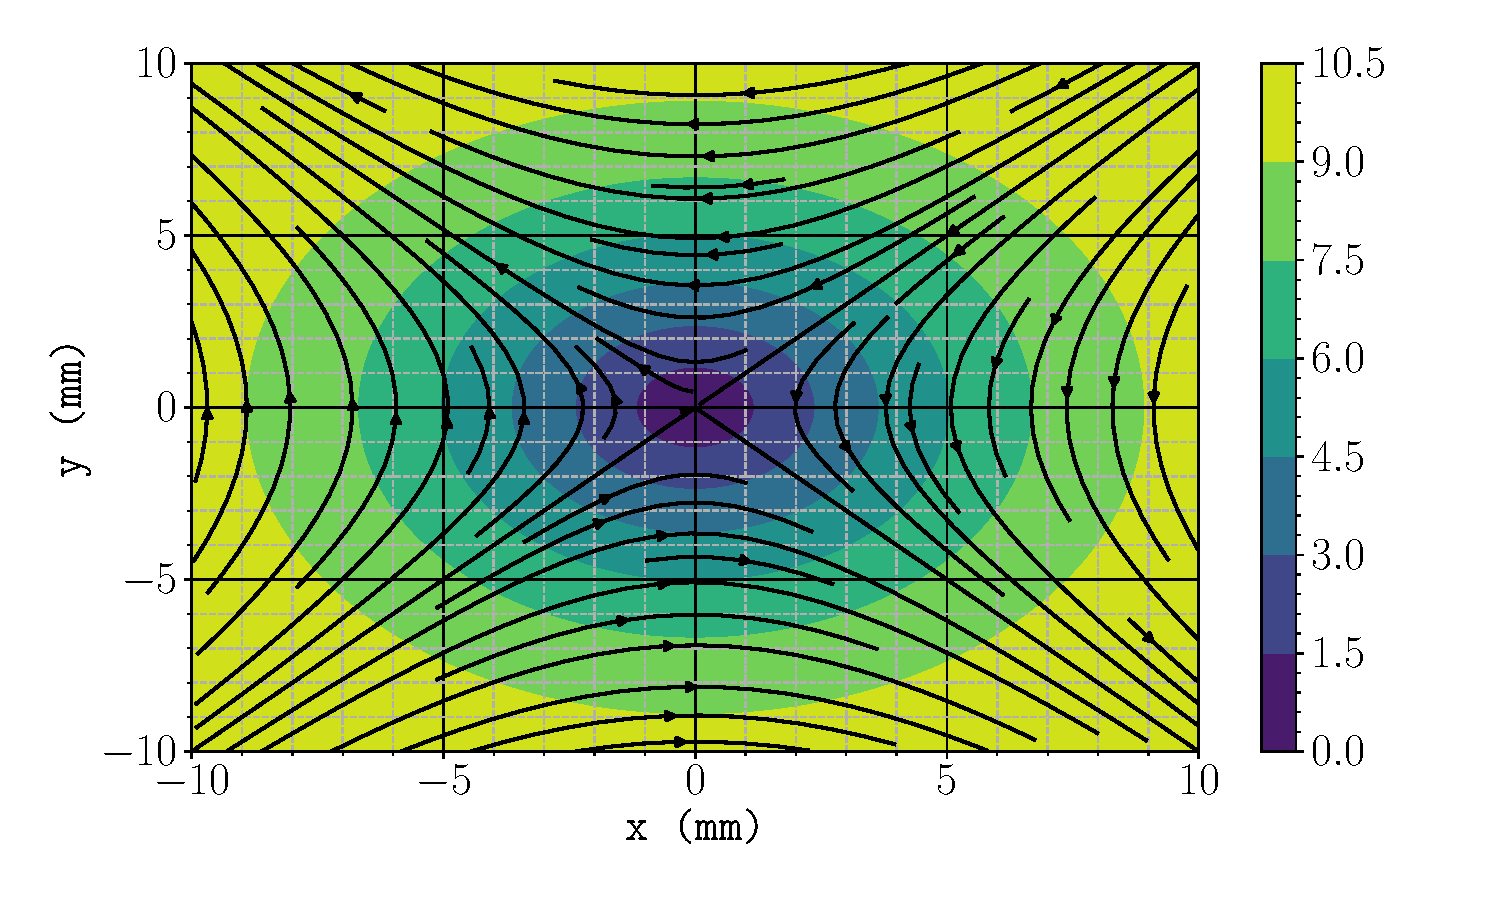
\includegraphics{3D_field_xy.pdf}\label{fig:3D_mot_radial}}}\\
	\caption[Simulated magnetic field for the 3D \ac{mot} quadrupole
		coils]{Simulated magnetic field for the 3D \ac{mot} quadrupole coils. In
		this coordinate system, the axial direction is defined as the
		\(\vec{z}\) axis. The simulation was performed using a nominal current
		of \sivalue{2.53}{\ampere}, which corresponds to a current density in
		each coil of \sivalue{1.33}{\ampere\per\square\milli\metre}. The
		magnitude of the magnetic field (in units of \sivalue{}{\gauss}) and its
		direction in the axial and radial planes of symmetry are shown in
		\textbf{(a)} and
		\textbf{(b)}, respectively.}
	\label{fig:3D_mot_field_sim}
\end{figure}
\subsubsection{Bias Coils}
Three orthogonally arranged pairs of Helmholtz coils are used during the
experiment to provide a homogeneous magnetic field close to the centre of the chamber. In the initial loading and molasses stages, these are used to zero the magnetic field at the centre of the chamber. This is required for effective sub-Doppler cooling~\nocite{Walhout1992}. In subsequent stages,
these coils provide a bias field along the appropriate axes during state
preparation, interferometry and state detection. Each coil was wound using
\sivalue{1}{\milli\metre} thick wire and consisted of 5 axial and 10 radial
turns. For a pair of coils in Helmholtz configuration, the magnetic field
gradient at the centre is minimised when the axial separation \(a\) is equal to
the coil radius \(r\), but the geometry of the vacuum chamber meant that it was
not possible to satisfy this condition. The radii and axial separations of each
coil pair is presented in \TableRef{tab:bias_coils}.\begin{table}
	\begin{tabular}{|c|c|c|c|c|}
		\hline
		Axis        & \(a\) (mm) & \(r_i\) (mm) & \(r_o\) (mm) \\
		\hline
		\(\vec{x}\) & 88         & 105          & 115          \\
		\(\vec{y}\) & 132        & 178          & 188          \\
		\(\vec{z}\) & 116        & 123          & 133          \\
		\hline
	\end{tabular}
	\caption[Table of parameters for each 3D \ac{mot} bias coil.]{Table of
		parameters for each 3D \ac{mot} bias coil. \(a\) denotes the axial
		separation between each coil, \(r_i\) and \(r_o\) are the inner and
		outer radii.}
	\label{tab:bias_coils}
\end{table}
\subsection{CCD Imaging}\label{sec:imaging}
During the experiment, atoms are imaged using a CCD camera to spatially resolve the cloud. This was done to measure the temperature using a ballistic expansion method and the trajectory of the cloud (see~\SectionRef{subsec:molasses_imaging}). \FigureRef{fig:imaging_optics} shows a
diagram of the apparatus used for imaging. A pair of \sivalue{125}{\milli\metre}
and \sivalue{50}{\milli\metre} focal length lenses are used to image the cloud
onto a Pike F505-B CCD camera. The camera has a maximum resolution of \(2452 \times
2054\) pixels. A measurement of the magnification of a ruler gave a calibration factor of
\sivalue{7.065\pm 0.07}{pixel\per\milli\metre}. To reduce the level of background light on the CCD, a bandpass filter is placed in front of the sensor. This transmits \sivalue{780}{\nano\metre} light at an
efficiency of 60\%.
\begin{figure}[!htbp]
	\centering
	\def\svgwidth{0.6\textwidth}
	\input{Figures/Chapter4/ccd_optics.pdf_tex}
	\caption[Optical setup for CCD imaging]{Optical setup for CCD imaging. Two
		lenses are used to magnify the image of the atom cloud on the CCD. A
		bandpass filter is placed in front of the sensor to block out background
		light at wavelengths other than
		\sivalue{780}{\nano\metre}. All lengths are given in millimetres.}
	\label{fig:imaging_optics}
\end{figure}
\subsubsection{Incident Optical Power Calibration} 
Measuring the incident optical power is useful for estimating the
number of atoms \(N_a\) by measuring the amount of light emitted
during resonance fluorescence. However, typical number densities in a
\ac{mot} mean that incident light is strongly absorbed by atoms close
to the surface. Consequently, the
assumption of a constant scattering rate per atom is not valid and leads to an
under-estimate of the atom number. More accurate techniques such as
absorption imaging can be used, but for the purposes of this
experiment, it was
sufficient to use fluorescence imaging as a rough estimate of the
number of atoms in the \ac{mot}. In subsequent stages of the
experiment, a sensitive photodiode with a high bandwidth was used to
detect the atoms in each hyperfine ground state. Details on this setup
can
be found in~\SectionRef{subsec:photodiode_setup}. \par\noindent
Under the assumption that the
power radiated per atom is constant, the power incident on the CCD
\(P_\textnormal{ccd}\) can be related to the scattering rate per atom as follows
\begin{equation}
	P_\textnormal{ccd} = \frac{\Omega}{4\pi} t R_\textnormal{sc}  \hbar \omega N_a
\end{equation}
where $\Omega/4\pi = $\pow{1.8}{-3} is the fractional solid angle subtended by
the imaging optics, \(t\) is the transmission of the bandpass filter
and 
\(\hbar \omega =
\sivalue{1.6}{\electronvolt}\) is the emitted photon energy. For a
two-level system, the scattering rate $R_\textnormal{sc}$ is 
\begin{equation}
  \label{eq:scattering_rate}
  R_\textnormal{sc} = \frac{\Gamma}{2} \frac{s}{1+s+\left(\frac{2
  \delta}{\Gamma}\right)^2}
\end{equation}
where $\Gamma$ is the natural linewidth of the transition, $\delta$ is
the frequency detuning and $s = I/I_\textnormal{sat}$ is the
saturation parameter. This incident power
is then related to the integrated number of pixel counts \(C_\textnormal{int}\)
by
\begin{equation}
	C_\textnormal{int} = \alpha \tau_\textnormal{exp} \eta P_\textnormal{ccd}
\end{equation}
where \(\tau_\textnormal{exp}\) is the exposure time, \(\eta = 0.14\) is the
quantum efficiency of the CCD and \(\alpha\) is a scaling factor that relates
the total charge collected to the total number of pixel counts. By varying the
exposure time used to image a collimated beam with a total power of
\sivalue{0.17}{\micro\watt}, the total number of counts recorded by the camera
as a function of exposure time is plotted in~\FigureRef{fig:camera_counts}. This
gives a count scaling factor of \(\alpha\) =
\pow{2.2}{5}\,counts\,\sivalue{}{\per\micro\second\per\micro\watt}.
\begin{figure}[!htbp]
	\centering
	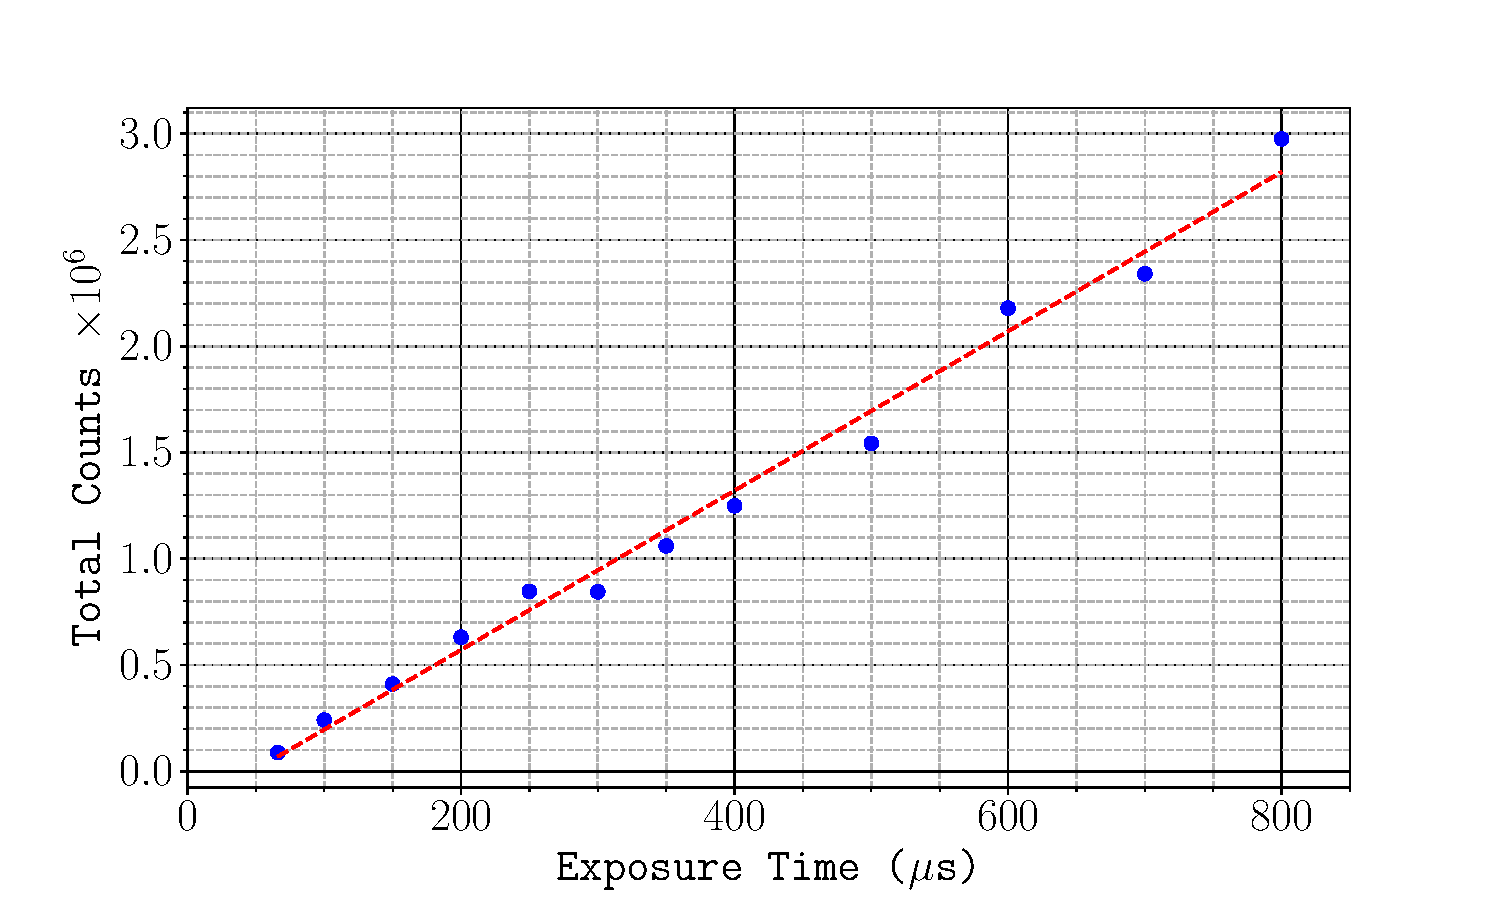
\includegraphics[width=0.5\textwidth]{cam_per_exposure}
	\caption[Integrated pixel counts as a function of CCD exposure
		time.]{Integrated pixel counts as a function of CCD exposure time for an
		incident optical power of \sivalue{0.17}{\micro\watt}. The dashed line
		indicates a linear regression which gives a scaling factor of \(\alpha\)
		=
		\pow{2.2}{5}\,counts\,\sivalue{}{\per\micro\second\per\micro\watt}.}
	\label{fig:camera_counts}
\end{figure}

\section{Generating MOT light}\label{sec:muquans_light}
 All the \ac{mot} light in this experiment was generated by the
 \Muquans\
laser~\cite{muquansWebPage}. \Muquans\ is a French laser company that is a
spin-off from the Institut d'Optique and Observatoire de Paris. A
schematic of
this laser system is shown in \FigureRef{fig:muquans_schematic}. The
light is fibre-coupled to minimise the number of free-space optical components.
This makes the system more stable in the presence of vibrations and
temperature variations. The \Muquans\ laser is comprised of four
\sivalue{1560}{\nano\metre} \acp{ecdl} which are frequency-doubled to produce
light at
\sivalue{780}{\nano\metre}~\cite{Menoret2011}\nocite{Leveque2014}. The first acts as a master laser
which is locked to the \trans{3}{3,4} crossover point in
\ac{rb85} to serve as an absolute frequency reference. The other three slave
lasers are used for output. The first one provides light for cooling \ac{rb87} using the \trans{2}{3} transition.
Light for the \trans{1}{2} repump transition is created by phase modulating this laser using an \ac{eom}.
The other two make up a pair of lasers for driving Raman transitions. One laser
is frequency-offset locked to the master and the other is phase-locked to the
first. This Raman laser was not used in this experiment, so will
not be discussed in further detail. The power in each of these slave lasers is amplified using
an \ac{edfa}. The frequency is doubled to around \sivalue{780}{\nano\metre} using a \ac{ppln}. The output power is controlled using an
\ac{aom}.
\begin{figure}[!htbp]
	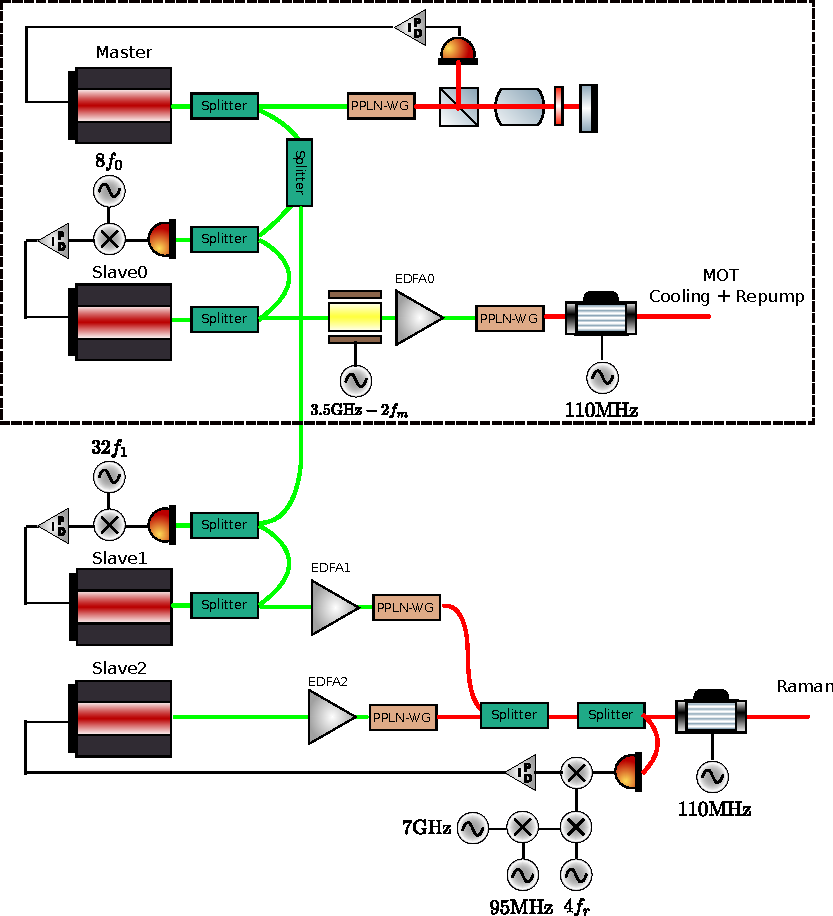
\includegraphics[width=0.8\textwidth]{muquans_schematic}
	\caption[\Muquans\ Laser System Diagram]{Schematic of the \Muquans\ laser system. Each output laser is derived from a\sivalue{1560}{\nano\metre} \acs{ecdl} (shown in green) which is amplified using an \acs{edfa} and then frequency-doubled to \sivalue{780}{\nano\metre} using a \acs{ppln} crystal. A master laser is locked to the 3,4 crossover in \ac{rb85} and the output lasers are offset-locked to their corresponding frequencies. The dashed region indicates the components used for generating light for the \acp{mots}, which was the only function of this laser for this experiment.}\label{fig:muquans_schematic}
\end{figure}
\subsection{Absolute Frequency Reference}\label{subsec:muquans_master}
The master laser provides an absolute frequency to which the slave
lasers are offset-locked. The reference frequency is created using 
saturated absorption spectroscopy inside a Rubidium vapour cell. The sub-Doppler
features in this spectrum are insensitive to temperature changes, and under
have linewidths closer to the natural linewidth of
Rubidium (\(\Gamma \sim 2\pi \times 6\) MHz). \FigureRef{fig:muquans_satspec}
shows the saturated absorption spectrum using the \Muquans\ master laser. The frequency is varied
by finely adjusting the temperature of the master \ac{ecdl}. The
master laser is set to lock to the crossover resonance between the \(F = 3
\rightarrow F' = 3\) and \(F = 3 \rightarrow F' = 4 \) transitions in \ac{rb85}
(indicated as \textbf{(b)}), which is the strongest feature in the spectrum. This
absorption feature is around \sivalue{1.1}{\giga\hertz} below the cooling
transition in \ac{rb87} (indicated as \textbf{(a)}).
\begin{figure}[!htbp]
	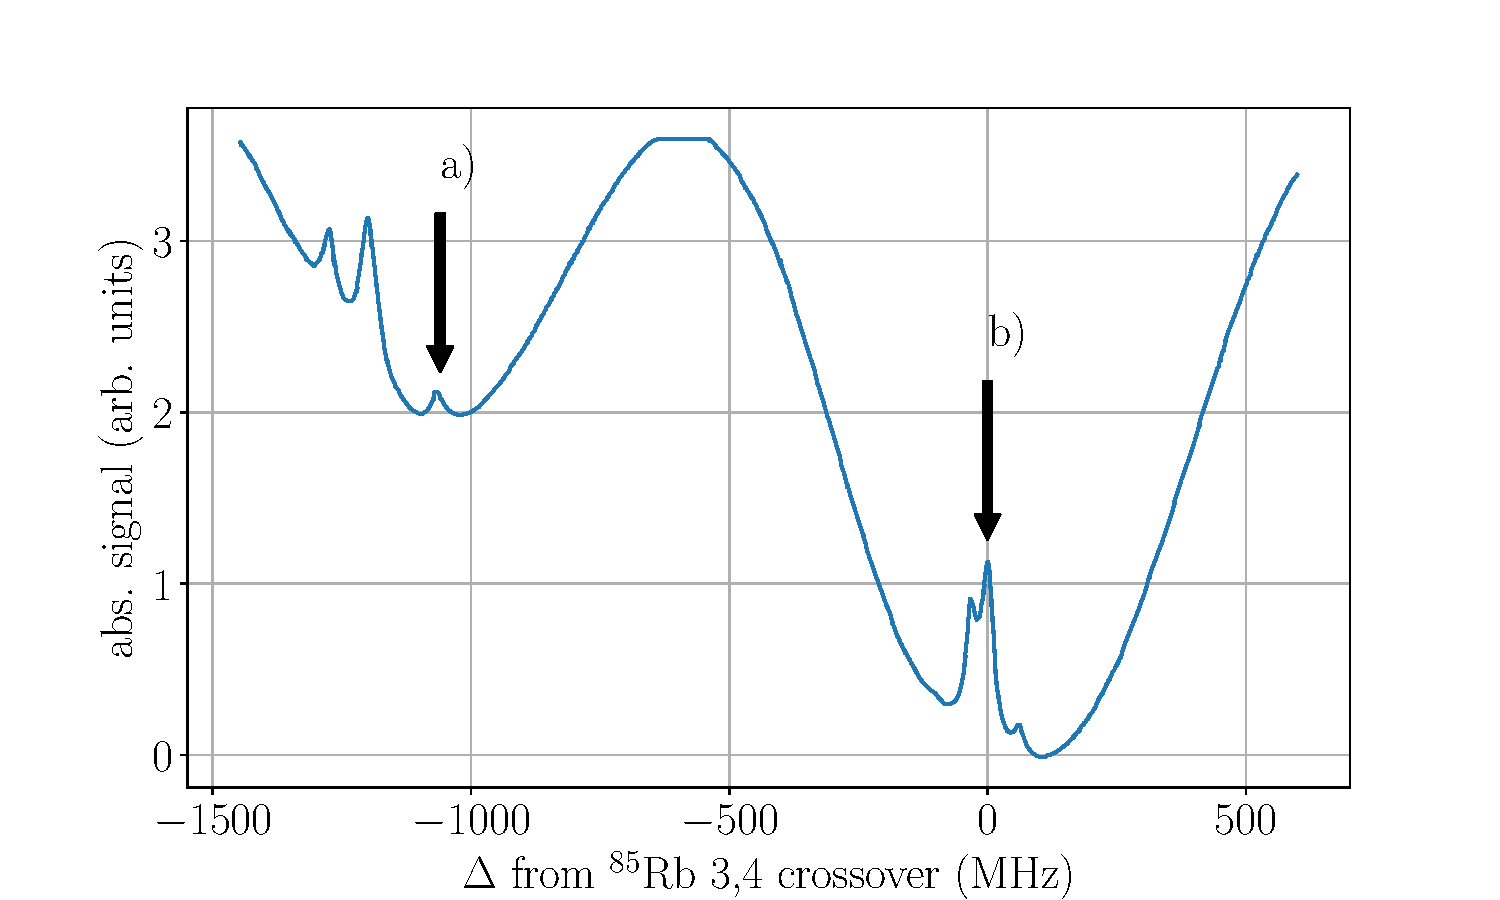
\includegraphics[width=0.6\textwidth]{sat_spec}
	\caption[Saturated absorption spectroscopy of the \\Muquans\ master laser.]{Saturated absorption spectroscopy using the Rubidium vapour cell in the \Muquans\ laser. The absorption features indicated are \(a\): the \(F = 2 \rightarrow F' = 3\) transition in \ac{rb87} and \(b\): the crossover resonance between the \(F = 3 \rightarrow F' = 3\) and \(F = 3 \rightarrow F' = 4 \) transitions in \ac{rb85} which is used to lock the frequency of the master laser.}\label{fig:muquans_satspec}
\end{figure}
\begin{figure}[!htbp]
	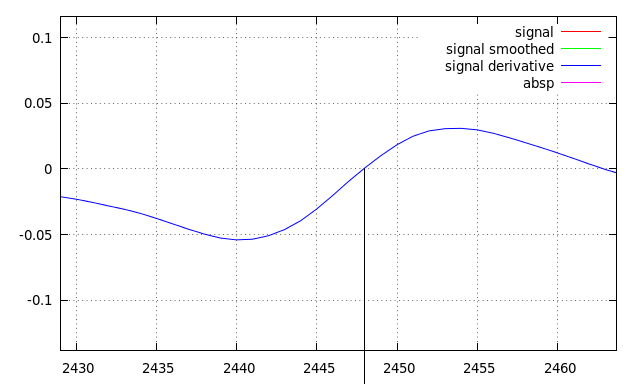
\includegraphics[width=0.6\textwidth]{error_signal}
	\caption[Error Signal for the \Muquans\ master servo.]{Error signal obtained by modulating the laser current. Close to the lock point, the signal is approximately linear. This signal is used in a feed-back loop to correct for frequency changes of the master laser.}\label{fig:muquans_error_signal}
\end{figure}
The frequency of the laser is modulated by modulating the current to
the \ac{ecdl}~\cite{Supplee1994}. This produces a signal that is
proportional to the frequency difference from the lock point. The error signal shown in
\FigureRef{fig:muquans_error_signal} is obtained by demodulating the absorption
signal using a lock-in amplifier. The servo that controls the master laser frequency also contains
an integrator to compensate for long-term drifts arising from temperature
variations.
\subsection{Cooling and Repump Light}
The first of the slave lasers provides light to address the cooling
transition. This is
frequency-offset locked to the master by comparing their beat frequency to a
reference from a \ac{dds}. A plot of the error signal used to lock this offset
frequency is shown in \FigureRef{fig:slave_offset}.
\begin{figure}[!htbp]
	\centering
	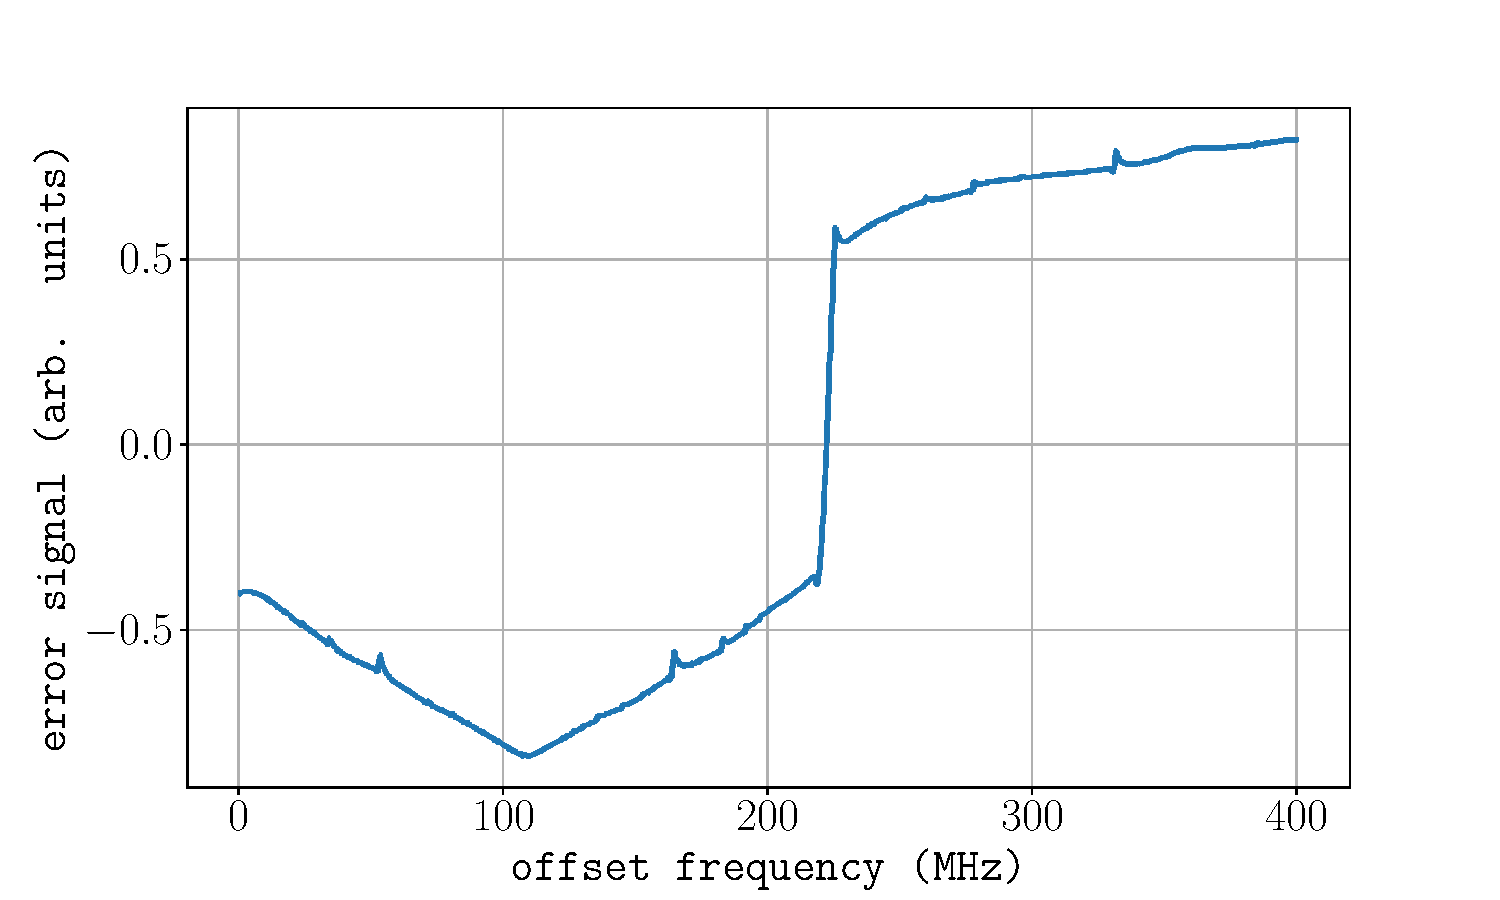
\includegraphics[width=0.6\textwidth]{slave0_error}
	\caption[Error Signal for the \Muquans\ Cooling laser.]{Error signal for the \Muquans cooling laser, plotted as a frequency difference from the start of the scan. This is obtained by comparing the beat frequency between the master and slave lasers to a reference frequency generated by a \ac{dds}. A servo loop feeds-back onto the frequency of the slave laser to keep this difference close to zero.}\label{fig:slave_offset}
\end{figure}
\par\noindent An \ac{eom} modulates the phase of the cooling laser to
produce light for the \trans{1}{2} repump transition. This modulation
creates frequency sidebands separated by integer multiples of the
modulation frequency
\(f_m\). If the amplitude of the modulation is small, only the first
positive and negative sidebands are present. A separate \ac{dds} provides the reference for the modulation frequency, so that the frequency of the cooling and repump
light can be independently ramped during the experiment (see
\SectionRef{subsec:muquans_comm}). This is amplified, doubled and subtracted
from a \sivalue{3.5}{\giga\hertz} reference signal so that the positive
frequency sideband is approximately \sivalue{6.6}{\giga\hertz} above that of the
cooling light, to address the repump transition. The modulation power is externally controlled using a \ac{vca} to control the ratio of
repump power to cooling power. An RF switch turns the repump on and off by blocking the reference frequency. \par\noindent The total output power is controlled using an
\ac{aom} that has a fixed modulation frequency of
\sivalue{110}{\mega\hertz}. \FigureRef{fig:muquans_cooling} shows
the combined power of the cooling light for the 3D \ac{mot} as a
function of the control voltage to the \ac{aom}
RF power. The hardware used to divide the light from the laser to the
separate beams is described in~\SectionRef{subsec:optical_fibre}.
\begin{figure}[htpb]
  \centering
  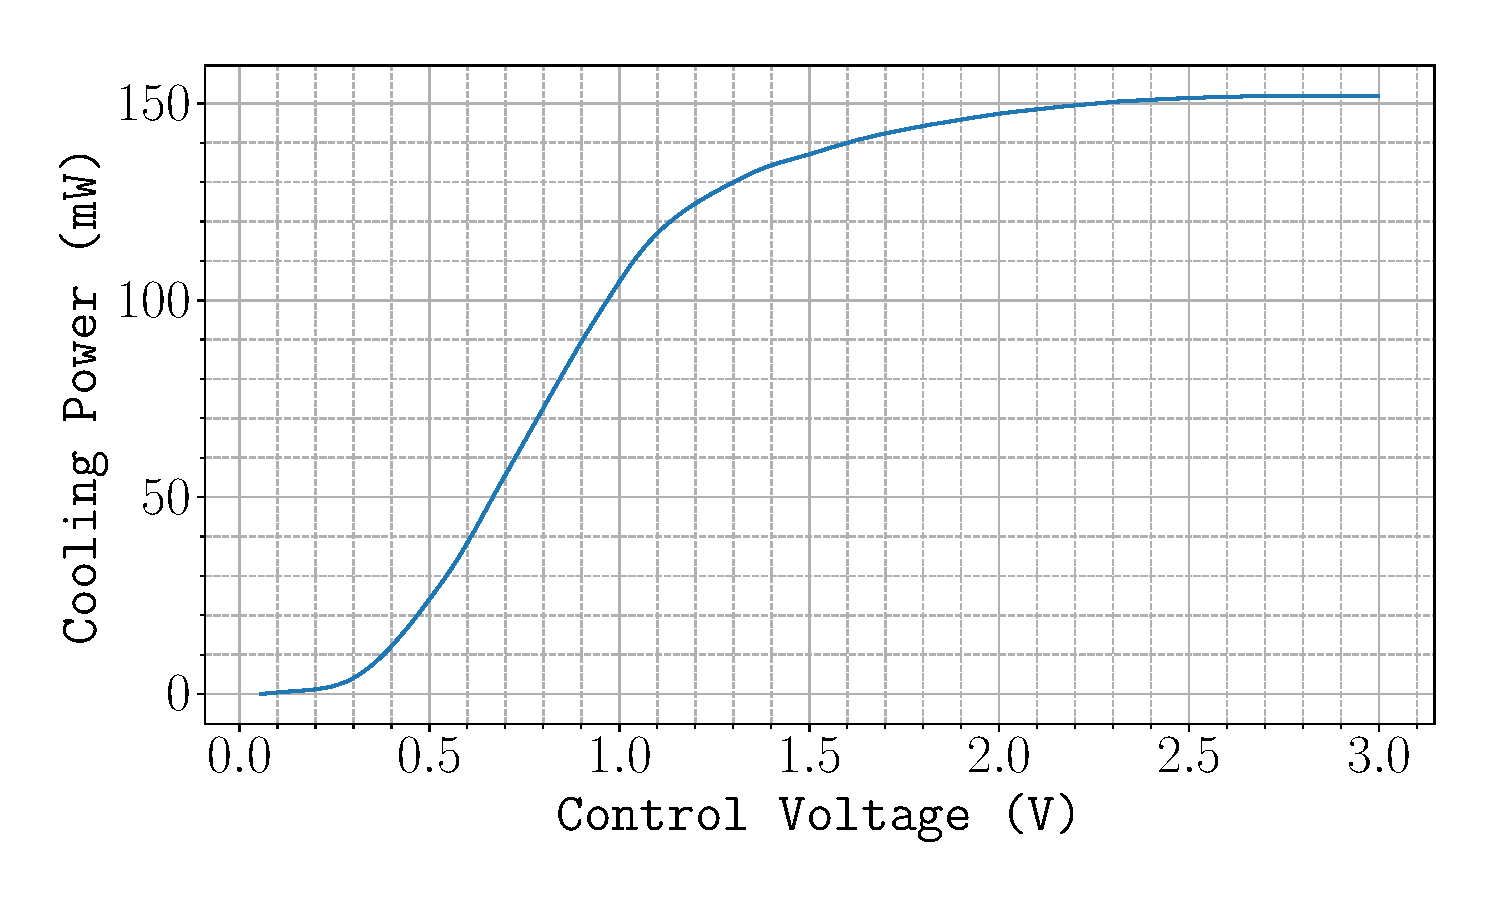
\includegraphics[width=0.8\linewidth]{muquans_cooling.pdf}
  \caption[Cooling power vs. \ac{aom} control voltage.]{Combined
  3D \ac{mot} cooling power as a function of control voltage for the
  RF power that drives the
\Muquans output \ac{aom}.}
  \label{fig:muquans_cooling}
\end{figure}
\subsection{Real-Time Control} \label{subsec:muquans_comm}
During the experiment, it is necessary to vary the frequency and power
of both
the cooling and repump light.
Analogue and digital signals control the RF sources for the output
\ac{aom} and
\ac{eom}. A \ac{dds} generates each RF frequency, so that they can be
updated in real-time.
These are also
programmed to ramp the output frequency for a specified duration and
ramp rate. This is done by sending serial messages to an
application which interprets the message and synchronously communicates the command to the \ac{dds} using
\ac{spi}. A glossary of the messages and their function is given
in~\AppendixRef{app:serial_commands}. The command is stored in memory
on-board the \ac{dds} and
is triggered to start using a digital pulse. This means that time at
which the frequency of the light changes is synchronised with the rest
of the experiment. 
\section{Controlling the MOTs}\label{sec:mot_control} Effective
trapping and cooling of Rubidium requires careful control of the light
and magnetic fields used to create the \ac{mot}. A well-balanced
\ac{mot} requires circularly polarised beams with equal intensities so
that there is no net force from scattering light. Otherwise, the
\ac{mot} forms at a position where the magnetic field is not
zero~\cite{Steane1992}. Equivalently, the \ac{mot} requires good
control of the magnetic field inside the chamber. What follows is a
description of the hardware used to implement this control.
\SectionRef{subsec:optical_fibre} describes the network of optical
fibres used to control the frequency and power in each \ac{mot} beam.
The electrical circuits used to control the strength of each bias
field, as well as switching off the quadrupole coils, are described
in~\SectionRef{subsec:coil_control} 
\subsection{Optical Fibre
Network}\label{subsec:optical_fibre} A network of fibre-based
beam-splitters and \acp{aom} distributes the light from the \Muquans
fibre to each of the beams for the 2D and 3D \acp{mot}. This provides
independent control of the power and frequency of the light at each
output of the fibre network. A diagram of this setup is shown
in~\FigureRef{fig:fibre_network}. The \Muquans fibre output is
polarised using a polarising beam-splitter before a \ac{hwp} aligns it
with the slow axis of a \ac{pm} fibre. The light is first divided on a
1:2 beam-splitter, with 66\% exiting one port, used for the 3D
\ac{mot}. The 34\% on the other port is split again using another 1:2
beam-splitter so that 95\% and 5\% of the power exits each port, for
the 2D \ac{mot} and push beam, respectively. Independent control each
output is done using a \textit{Gooch and Housego} fibre \acp{aom} with
a central modulation frequency of \sivalue{135}{\mega\hertz}. The
junctions between components are spliced together to minimise
insertion loss. The slow axes of each fibre are aligned so that the
polarisation of the input light is maintained. \par\noindent The light
for the 3D \ac{mot} is split using a 1:3 splitter into pairs of
outputs for the light along the \(\vec{x},\vec{y}\) and \(\vec{z}\)
axes. Unlike the outputs along the other axes, the ones used for light
along the \(\vec{z}\) axis have separate \acp{aom}. This is done so
that during the experiment, a single beam along the \(\vec{z}\) axis
can used to blow away background atoms (see
\SectionRef{subsec:blow_away} for more details).

\begin{figure}[!htbp] 
  \centering 
  \fontsize{18pt}{18pt}
  \resizebox{0.5\textwidth}{!}{\input{Figures/Chapter4/fibre_network.pdf_tex}}
  \caption[Network of optical fibre splitters and \acp{aom} for
  \ac{mot}light distribution]{Fibre splitter and \acp{aom} for
  \ac{mot} light distribution. The polarisation of the cooling and
repump light from the \Muquans laser is aligned to the fibre network
using a \ac{pbs} and \ac{hwp}. Apart from the outputs for the
\(\vec{x}\) and \(\vec{y}\) 3D \ac{mot} beams, which have a single
\ac{aom} per axis, the power and frequency at each output can be
controlled independently. The percentages shown are the relative power
at each output, accounting for insertion loss and driving each
\ac{aom} with the optimum RF power.} 
\label{fig:fibre_network}
\end{figure} 
\subsection{Magnetic Field Control}\label{subsec:coil_control} 
The current through each set of
bias coils (3 for the 3D \ac{mot} and 2 for the 2D \ac{mot}) is
controlled using a voltage-controlled current source. The control
voltage is an input at the non-inverting terminal of an OPA549 op-amp.
The coils are placed in series with a sense resistor of resistance
\(R_s\) at the output. The circuit is configured to that the voltage
at the inverting terminal is \(V_- = i R_s\).  This forms a negative
feed-back loop to keep the output current constant if the load
resistance changes. The bias coils can be supplied with up to
\sivalue{2}{\ampere} using a control voltage of \sivalue{10}{\volt}.
\par\noindent This same circuit is used to control the 3D \ac{mot}
coils, except for the fact that their larger resistance necessitates a
larger gain to achieve the current necessary to produce a strong field
gradient. During the experiment, the 3D \ac{mot} coils need to be
switched off rapidly, to allow for effective sub-Doppler cooling of
the atoms~\cite{Dedman2001}. The coils are an inductive load, so the time taken for the
current to decay is determined by the time constant \(\tau = L/R\).
With a negative voltage across them, the stored energy (and hence,
magnetic field) dissipates at a faster rate. A flux-gate magnetometer
was used to measure the time taken to switch off the coils. With an
applied voltage of \sivalue{0}{\volt}, the characteristic decay time
is \(\tau = \) \sivalue{2.5}{\milli\second}. Under the maximum
available back-EMF of \sivalue{-24}{\volt}, the field can be
completely switched off in \sivalue{800}{\micro\second}. \par\noindent
The quadrupole coils for the 2D \ac{mot} are switched off in much the
same way. An IGBT cuts the flow of current when the gate voltage drops
below a threshold value. To prevent damage to the transistor, a diode
and \sivalue{10}{\ohm} power resistor are placed in parallel with the
coils. This allows the current generated by the back-EMF to dissipate
without damaging the IGBT. These field from these coils can be
switched off in less than \sivalue{1}{\milli\second}.

\section{Characterising the MOTs}\label{sec:mot_characterisation}
This section discusses the performance of the 2D and 3D \acp{mots} for trapping
and cooling \ac{rb87}. The main goal of this stage of the experiment is to
quickly produce an ensemble of trapped, cold atoms in the 3D \ac{mot}. For this
reason, the loading rate of the 3D \ac{mot} is a useful figure-of-merit. As
further cooling in an optical molasses is necessary to achieve a sufficiently
cold ensemble for interferometry (see \SectionRef{sec:optical_molasses}), the
temperature of atoms in the \ac{mot} will not be discussed in detail.
\par\noindent \nocite{Haw2012}
At the start of the experiment, the light and magnetic fields to produce the 2D
and 3D \acp{mots} are switched on. \TableRef{tab:mot_parameters} shows
typical values for the cooling and repump power, as well as the field gradients
and bias fields used. The cooling light is detuned by \(-2 \Gamma\) from the
\trans{2}{3} transition for the 2D \ac{mot} and by\(-2.5 \Gamma\) for the 3D
\ac{mot}. The push beam is at resonance. A timing diagram of the loading sequence is given in~\FigureRef{fig:mot_loading_timing}. The light and magnetic fields
for the 2D \ac{mot} are switched off after \sivalue{100}{\milli\second} and the
3D \ac{mot} is kept on for a further \sivalue{50}{\milli\second} to allow for
the transit of the remaining atoms from the 2D \ac{mot} to the 3D \ac{mot}.
After a sufficient number of atoms are loaded, the experiment proceeds by
switching off the 3D quadrupole field prior to cooling in an optical molasses.
\begin{table}[!hbtp]
	\centering
	\begin{tabular}{@{}llllllll@{}}
		\toprule
		\multicolumn{4}{c}{2D MOT}           & \multicolumn{4}{c}{3D MOT}
		\\
		\midrule
		\multicolumn{2}{l}{Laser Power}      & \multicolumn{2}{l}{Magnetic
		Field}                               & \multicolumn{2}{l}{Laser Power}
		& \multicolumn{2}{l}{Magnetic Field}
		\\
		Cooling                              & \sivalue{60}{\milli\watt}
		& \(\mathrm{d}\vec{B}/\mathrm{d}\rho\) &
		\sivalue{18}{\gauss\per\centi\metre} & Cooling                              & \sivalue{130}{\milli\watt}
		                                     & \(\mathrm{d}\vec{B}/\mathrm{d}z\)
		                                     &
		                                     \sivalue{15}{\gauss\per\centi\metre}
		                                     \\
		Repump                               & \sivalue{6}{\milli\watt}
		                                     & \(B_x\) & \sivalue{0.48}{\gauss}
		                                     & Repump
		                                     & \sivalue{13}{\milli\watt} &
		                                     \(B_x\) & \sivalue{1}{\gauss}
		                                     \\
		Push                                 & \sivalue{500}{\micro\watt}
		& \(B_y\)                              & \sivalue{-0.46}{\gauss}
		&                                    &                           &
		\(B_y\) & \sivalue{-0.5}{\gauss}
		\\
		                                     &
		                                     &
		                                     &                           &
		                                     &   & \(B_z\) &
		                                     \sivalue{0.22}{\gauss}
	\end{tabular}
  \caption[Typical optical and magnetic parameters for the
  \acp{mots}.]{Typical optical and magnetic parameters used for the 2D
  and 3D \acp{mots}. The optical powers listed are the total used for
each \ac{mot}, which is divided into separate beams. The bias field
strengths are the values used during the preliminary trapping stage of
the experiment. The specified field gradients are given along the
radial direction and the symmetry axis of the quadrupole coils for the
2D and 3D \acp{mots}, respectively.}
  \label{tab:mot_parameters}
\end{table}
 \begin{figure}[!htbp] \centering %\def\svgwidth{0.6\textwidth}
   \resizebox{0.7\textwidth}{!}{\input{mot_loading_timing.pdf_tex}}
   \caption[\ac{mot} loading timing diagram.]{Timing diagram for the loading stage of the experiment. The 2D \ac{mot} is switched on for \sivalue{100}{\milli\second} and is switched off earlier than the 3D \ac{mot}. }
   \label{fig:mot_loading_timing} 
\end{figure}
\subsection{3D MOT Loading Rate}\label{subsec:loading_rate}
The loading rate of the 3D \ac{mot} from a beam of atoms originating from the 2D
\ac{mot} can be understood using the following rate equation
\begin{equation}
	\frac{\mathrm{d} N}{\mathrm{d}t} = R  \phi_\textnormal{rb} - \left(\alpha \phi_\textnormal{rb}  + \beta n_\textnormal{bg} \right) N - \gamma N^2
	\label{eq:loading_rate}
\end{equation}
where \(\phi_\textnormal{rb}\) is the flux of rubidium through 3D \ac{mot}
capture volume and \(R\) describes the rate at which rubidium is cooled and
trapped such that \( R \phi_\text{rb}\) is the loading rate of the 3D \ac{mot}.
The second term describes a loss rate due to collisions between trapped atoms
and untrapped rubidium and background atoms. These loss rates are parameterised
by \(\alpha\) and \(\beta\), respectively. The final term describes the loss of
atoms from the trap due to intra-trap collisions~\cite{Prentiss1988} which
depends on the density of atoms in the trap. In the case of a large flux of
atoms from the 2D \ac{mot} the first two terms dominate, leading to a simple
solution for the number of atoms in the 3D \ac{mot}
\begin{equation}
	N(t) = \frac{R \phi _{\text{rb}} \left(1-e^{-t \left(\beta  n_{\text{bg}}+\alpha  \phi _{\text{rb}}\right)}\right)}{\beta  n_{\text{bg}}+\alpha  \phi _{\text{rb}}}
	\label{eq:atom_number}
\end{equation}
which has a steady-state atom number given by
\begin{equation}
	N_\infty = \frac{R \phi _{\text{rb}}}{\beta  n_{\text{bg}}+\alpha  \phi _{\text{rb}}}
\end{equation}
Under a small atomic flux, both the loading rate and steady-state atom number
increase as the flux of atoms from the 2D \ac{mot} increases. Once this flux is
great enough, the loss due to background atom collisions is small compared to
the loss due to rubidium collisions and the final number is independent of
\(\phi_\text{rb}\). \par\noindent The flux of atoms from the 2D \ac{mot} depends on the 2D
\ac{mot} loading rate, which in turn depends on the capture volume and rubidium
number density inside the cell.  Without any longitudinal cooling, a significant
fraction of atoms leaving the cell will have a velocity greater than the 3D
\ac{mot} capture velocity~\cite{Schoser2002}. \par\noindent The effect of
varying the partial pressure of rubidium inside the source cell is shown
in~\FigureRef{fig:loading_plots}. The number of atoms in the 3D \ac{mot} was measured over time for a range of dispenser currents. At low partial pressures,
the loading rate increases due to the increase in the flux from the 2D \ac{mot}.
As the pressure increases, the increasing flux gives a larger steady-state
number of atoms, up until the background pressure becomes negligible.
\FigureRef{fig:loading_nopush} and \FigureRef{fig:loading_push} compare the loading
curves observed with and without the push beam. Below a threshold pressure, the
push beam greatly improves the loading rate since a greater fraction of the
atoms can be captured in the 3D \ac{mot}. 
\par\noindent \FigureRef{fig:loading_rate} shows the
fitted loading rate for each scenario. There is a clear optimum pressure,
where the loading rate is \sivalue{2.4e9}{\per\second}. The steady-state atom number is
independent of the flux from the 2D \ac{mot}. Above this pressure, the loading rate is
sharply reduced. The increased collision rate between cold atoms from the 2D
\ac{mot} and hot untrapped ones reduces the atomic flux. This also increases the
mean velocity of atoms in the beam, since faster ones are less likely to collide
with a background atom before exiting the cell. At very high pressures, the mean
velocity is so great that only a small fraction of atoms can be captured and the
push beam has little effect on the loading rate.
\begin{figure}[!htbp]
	\centering
	\def\svgwidth{\columnwidth}
	\subfloat[][]{\scalebox{0.3}{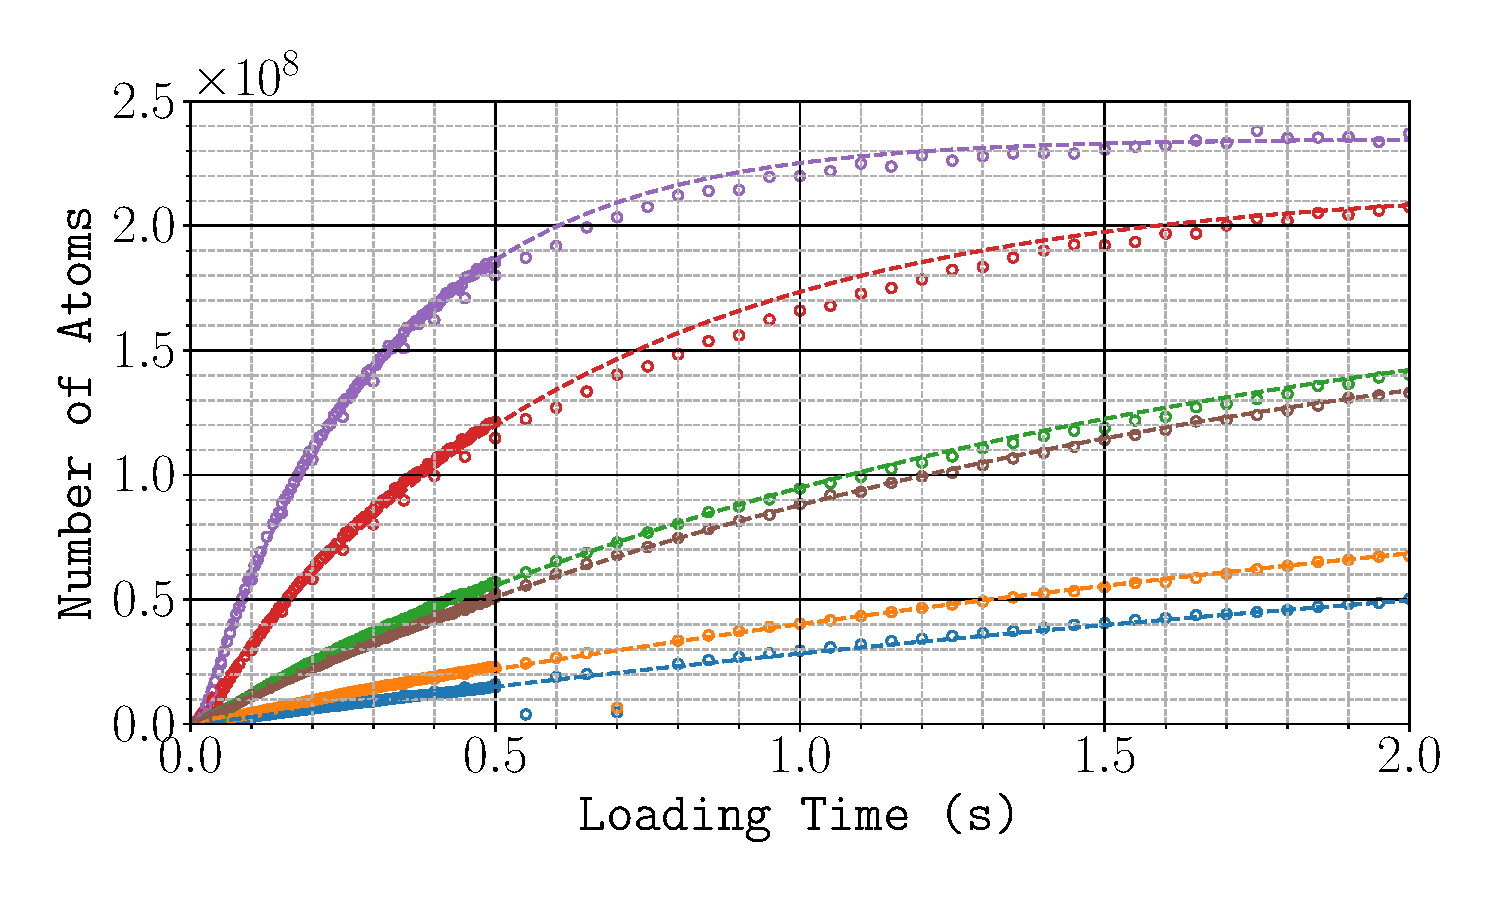
\includegraphics{Figures/Chapter4/loading_nopush.pdf}}\label{fig:loading_nopush}}
	\subfloat[][]{\scalebox{0.3}{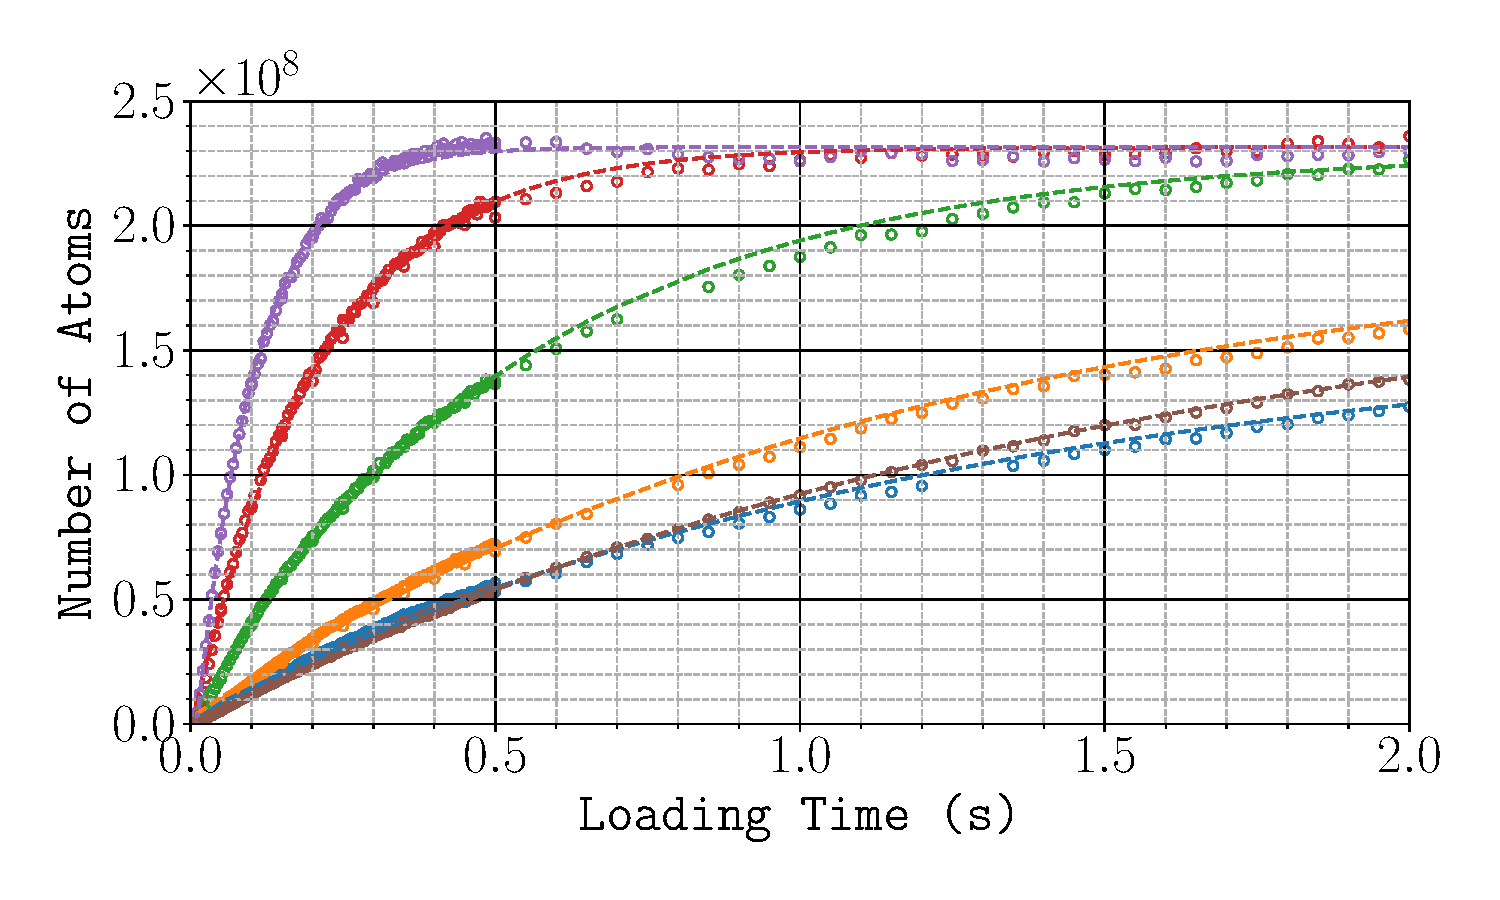
\includegraphics{Figures/Chapter4/loading_push.pdf}}\label{fig:loading_push}}\\
	\subfloat[][]{\scalebox{0.3}{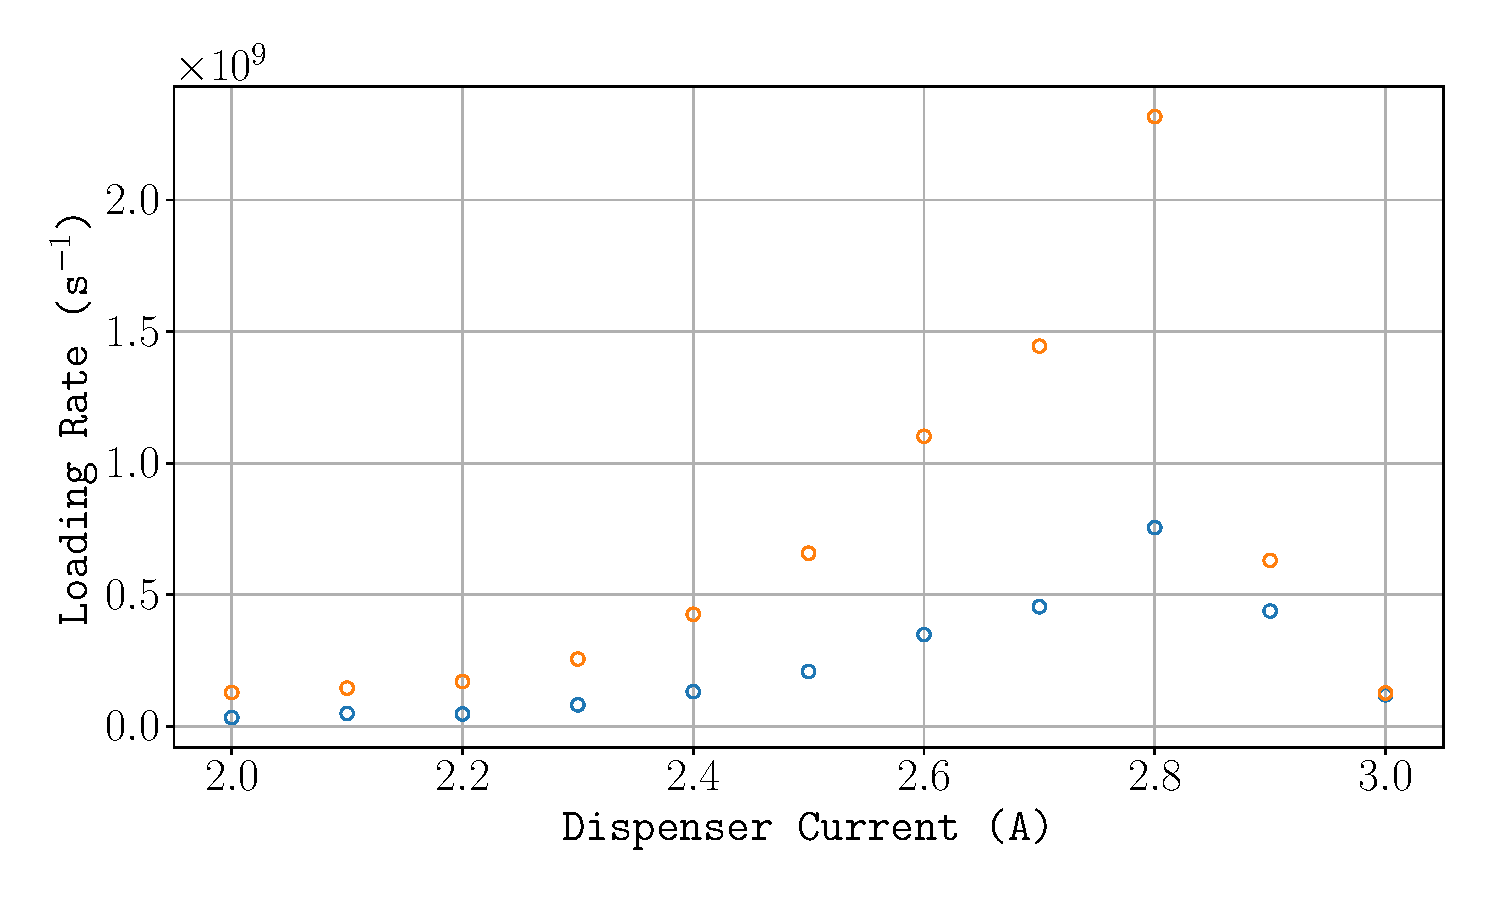
\includegraphics{Figures/Chapter4/loading_rate.pdf}}\label{fig:loading_rate}}
	\caption[3D \ac{mot} atom number vs dispenser current with and without a
		push beam.]{Number of atoms in the 3D \ac{mot} over time for a range of
		dispenser currents. For clarity, only the loading curves for dispenser
		currents of
		\sivalue{2}{\ampere} (blue),\sivalue{2.2}{\ampere}
		(orange), \sivalue{2.4}{\ampere} (green), \sivalue{2.6}{\ampere} (red),
		\sivalue{2.8}{\ampere} (purple) and \sivalue{3}{\ampere} (brown) are
		shown in \((a)\) and \((b)\), which present the number of atoms over
		time without and with a push beam, respectively. The loading rate (\(R
		\phi_\text{rb}\) in~\EquationRef{eq:loading_rate}) in both instances is
		shown in \((c)\). As the partial pressure of rubidium increases, the
		flux of atoms from the source cell increases. By longitudinally cooling
		the atoms, the push beam enhances the loading rate of the 3D \ac{mot}.
		Above a dispenser current of
		\sivalue{2.8}{\ampere}, the collision rate with hot untrapped atoms greatly reduces the atom flux, reducing both the loading rate and steady-state atom number.}
	\label{fig:loading_plots}
\end{figure}

\section{Conclusion}
This chapter has introduced the components of the experiment that were used to
trap and cool atoms in a \ac{mot}. This is used to prepare an ensemble of cold
atoms in a pure quantum state, suitable for interferometry. An optimisation of
the loading rate of the 3D \ac{mot} was carried out to reduce the dead time
between consecutive experiment cycles. 

    \chapter{Preparing Atoms for Interferometry}\label{chap:atom_prep}
\section{Chapter Overview}
This chapter presents the stages of the experiment which prepare an ensmble of atoms for interferometry, after they are loaded into the 3D \ac{mot}. After being released from the trap, the atoms are cooled and launched using a moving molasses, as described in~\SectionRef{sec:optical_molasses}. Following this, a sequence of optical and microwaves pulses are used to increase the population in the \(\ket{1,0}\) ground state and end with an ensemble which has a narrow velocity spread along the Raman axis. A characterisation of this is given in~\SectionRef{sec:state_prep}.
\par\noindent
Some sections of this chapter refer to parts of the experiment which have yet to be introduced. Details on the Raman laser and the velocity-selective Raman pulse can be found in~\SectionRef{sec:msquared_laser} and~\SectionRef{sec:raman_velocity_select}, respectively. A description of the detection scheme, used to measure the population of atoms in \(\ket{F=1}\) and \(\ket{F=2}\) is presented in~\SectionRef{sec:atom_detection}


\section{Cooling in Optical Molasses}\label{sec:optical_molasses}
{\textbf{Introduce motivation here}}
A low thermal velocity means that the atoms can be interrogated for a longer time and in the case of atom interferometry, leads to a more sensitive measurement of acceleration. In addition, the thermal expansion of the ensemble leads to greater systematic phase shifts due to effects such as magnetic field gradients and laser wavefront distortions. The temperature of atoms inside the \ac{mot} is greater than desired, so further cooling is required before a strong interferometer signal can be achieved. Temperatures well below that of the Doppler limit (\sivalue{146}{\micro\kelvin} for \ac{rb87}) can be reached using the dissipative force that acts on an atom travelling through a spatially varying electric field. 

\par\noindent
This section describes the work towards to cooling and launching the atoms in a moving optical molasses. It starts with a motivation for launching the atoms in~\SectionRef{subsec:launching}. The following section discusses the control of the intensity and frequency of the light during the molasses stage of the experiment. A description of the techniques needed to cool the atoms in a moving molasses is then given in~\SectionRef{subsec:moving_molasses}. Finally, this section concludes in~\SectionRef{subsec:molasses_imaging} with measurements of both the temperature and trajectory of the atom cloud which were measured using a ballistic expansion method.


\subsection{Motivation for Launching}\label{subsec:launching}
As previously discussed in~\SectionRef{sec:theory_double_int}, there are two pairs of counter-propagating beams which can drive Raman transitions between the two hyperfine ground states. If an atom can be stimulated by both pairs, then the additional trajectories this introduces do not interfere, resulting in a reduction in the fringe visbility. This problem can be avoided by using the fact that the Raman transition is Doppler-sensitive to ensure that the atoms are only driven by one pair of beams. Each pair has an opposite Doppler shift \(\pm \omega_D = \pm \keff.\textbf{v}\) and so their transition frequencies are separated by \(2\omega_D\). Therefore, the atoms are launched so that their centre-of-mass velocity along the Raman axis is large enough to lift the degeneracy of the two Raman transitions. 

%The light used to drive Raman transitions during the exeperiment is launched into the chamber on two orthogonal axes of a \ac{pm} fibre. These are retro-reflected to produce two counter-propagating beams that are orthogonally polarised to the incoming ones. In the absence of \(\pi\)-polarised light, only \((\sigma^+-\sigma^+)\) or \((\sigma^--\sigma^-)\) pairs of polarised beams can drive Raman transitions. If the incoming beams are circularly polarised, then this can occur using counter-propagating pairs of beams which impart momentum \(\pm \hbar \keff\) to an atom. If an atom can be driven by either pair at each interferometer pulse, this results in two interferometer paths, as well as additional trajectories which do not interfere and hence cause a reduction in fringe visibility.
\subsection{Frequency and Power Control}\label{subsec:molasses_control}
A timing diagram illustrating the power and frequency during this stage of the experiment is shown in \FigureRef{fig:molasses_timing}. After the atoms are loaded into the \ac{mot}, they are released by switching off the quadrupole field. Once this field has decayed away, the frequency and intensity of the cooling light are ramped adiabatically. The frequency of the cooling light is ramped to -25\(\Gamma\) over \sivalue{1.4}{\milli\second}. Since the repump light is generated using an \ac{eom}, the modulation frequency is simultaneously ramped up to keep this light resonant with the \trans{1}{2} transition. Additionally, the relative detuning of counter-propagating \ac{mot} beams is varied so that the atoms are cooled into a moving molasses (see~\SectionRef{subsec:moving_molasses}). After this, the intensity of the light is reduced over \sivalue{5}{\milli\second}. The response of the output \ac{aom} on the \Muquans laser was calibrated so that we could apply a voltage ramp that gives an approximately linear intensity ramp.
\begin{figure}
    \centering
    \resizebox{0.6\textwidth}{!}{\input{molasses_timing.pdf_tex}}
    \caption[Molasses stage timing diagram]{Timing diagram for the molasses stage of the experiment. After a time \(\tau_\text{a} = \sivalue{100}{\milli\second}\), the atoms are released from the \ac{mot}. The molasses sequence begins \sivalue{3}{\milli\second} later, once the magnetic field from the \ac{mot} coils has decayed away. First, the frequency of the cooling light is ramped to \(-25 \Gamma\) over \sivalue{1.4}{\milli\second}. The relative frequencies of counter-propagating \ac{mot} beams are detuned so that the atoms are cooled in a moving frame, launching them along a parabolic path (see~\SectionRef{subsec:moving_molasses}). Next, the intensity of the \ac{mot} light is reduced linearly over \sivalue{5}{\milli\second}. To measure the temperature, the atoms are left to expand for a duration of \(\tau_\text{exp}\) \sivalue{}{\milli\second}, after which they are imaged using the camera.}
    \label{fig:molasses_timing}
\end{figure}
\subsection{Launching in a Moving Molasses}\label{subsec:moving_molasses}

The configuration for launching atoms along the Raman axis is shown in \FigureRef{fig:moving_molasses}. The forward-propagating beams are blue-detuned by \(+\delta_l\) and the backward-propagating ones are red-detuned by \(-\delta_l\), so that atoms with a velocity along the beam axis of \(\vec{v} = \delta_l \lambda\) are+ resonant with both beams. The frequency of each beam is ramped from the initial value by varying the modulation frequency of its \ac{aom}. This ramp occurs slowly to ensure the atoms are adiabatically accelerated to the resonant velocity, minimising excess heating of the atoms. As there is no pair of \ac{mot} beams along the axis of the Raman beams, the \(\vec{x}\) and \(\vec{y}\) \ac{mot} beams, whose axes are nominally at 45\(^{\circ}\) to the Raman axis, are used to launch the atoms. By controlling the power and alignment of each beam, the net velocity on the atoms will be along the Raman axis. If the detuning of both pairs of beams is the same, then the velocity along the Raman axis is given by \(\vec{v_r} = \sqrt{2} \delta_l \lambda\)~\nocite{Ohshima1995}.
\begin{figure}
    \centering
    \def\svgwidth{0.6\textwidth}\input{moving_molasses.pdf_tex}
    %\resizebox{0.6\textwidth}{!}{\input{moving_molasses.pdf_tex}}
    \caption[Beam configuration for a moving molasses]{Beam configuration for a moving molasses. When counter-propagating beams are detuned from each other, the atoms are slowed to a velocity which balances the frequency of each beam. Along the vertical axis, the beams are detuned by \(\delta_v\) so that the cloud is launched upwards with a velocity \(v_z = \delta_v \lambda\). In the horizontal plane, the \(\vec{x}\) and \(\vec{y}\) beams are detuned by \(\delta_h\) so that the resultant velocity is along the Raman axis \(v_r = \sqrt{2}\delta_h\lambda\). }
    \label{fig:moving_molasses}
\end{figure}
\par\noindent
As well as launching the atoms horizontally, the atoms are launched vertically so that they do not fall as far under gravity. Since the atoms remain close to the centre of the beam, where the intensity across the cloud is more uniform, longer pulse separation times can be used before the intensity gradient causes a significant dephasing. This launch is carried out using the \ac{mot} beams that lie along the vertical \(\vec{z}\) axis. Under an appropriate choice of launch velocity, the centre-of-mass trajectory transverse to the Raman beam wavefront can be chosen to maximise the interferometer fringe visibility. This is presented in further detail in~\SectionRef{subsec:launch_contrast}. 
\par\noindent
\subsection{Imaging the Atom Cloud over Time}\label{subsec:molasses_imaging}
Once released from the trap, the atom cloud is free to expand. Provided that there are no external forces on the atoms from electric or magnetic fields, the expansion of the cloud is determined by its thermal velocity distribution. In addition to this, the centre-of-mass moves due to its initial velocity and acceleration due to gravity. For the purposes of this discussion, it is worthwhile to consider the motion of atoms within the ensemble separately to the centre-of-mass motion as these provide a means of measuring the temperature and launch velocity, respectively. These were measured by imaging the distribution of atoms after allowing the cloud to expand in the dark for a range of expansion times. A typical atom cloud trajectory is shown in~\FigureRef{fig:launch_images}, in which the cloud was imaged up to \sivalue{76}{\milli\second} after being released from the trap.

\begin{figure}
    \centering
    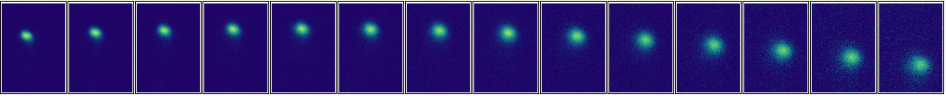
\includegraphics[width=0.8\textwidth]{molasses_launch}
    \caption[Atom cloud position after launching in a moving molasses]{A series of images showing the trajectory of the atom cloud after being cooled in a moving molasses. The first image was taken \sivalue{7}{\milli\second} after initiating the molasses and a subsequent one every \sivalue{5}{\milli\second}. Each image represents a region of interest of dimensions 1150 \(\times\) 1650 pixels that covers the spatial extent of the atom cloud during the launch.}
    \label{fig:molasses_launch}
\end{figure}
\subsubsection{Measuring the Temperature}
In thermal equilibrium, the velocity distribution of the atoms is described by a Maxwell-Boltzmann distribution
\begin{equation}
    f(v_x,v_y,v_z) = \left(\frac{m}{2\pi k_B }\right)^{3/2}e^{-\frac{m (v`_x^2+v`_y^2+v`_z^2)}{2 k_B T}}
    \label{eg:mb3D}
\end{equation}
where \(v`_i = v_i - \langle v_i \rangle\) is the difference from the average velocity. Along a single axis, the velocity distribution is obtained by integrating over the other velocity components. For the sake of notation, the following discussion uses \(x\) and \(v_x\) as labels for position and velocity, but these are interchangeable with the equivalent components along the other axes. As~\EquationRef{eg:mb3D} is a product of velocity distributions along each axis, the velocity distribution along one axis is 
\begin{equation}
    f(v_x) = \left(\frac{m}{2\pi k_B }\right)^{1/2}e^{-\frac{m (v_x-\langle v_x \rangle) ^2}{2 k_B T}}
    \label{eg:mb1D}
\end{equation}
Suppose that there are initially \(n_0 (x) \mathrm{d}x\) atoms within the region \((x, x+\mathrm{d}x)\), where \(n_0(x) = n(x, t=t_0)\) is the initial atomic density along one axis. During ballistic expansion, the atoms redestribute themselves according to their velocity. After a time \(t\) of free expansion, the position of an atom initially at \(x\) is \(x + v_x t\). 
Assuming that the number density is initially a Gaussian, with a peak number density \(n_0(x_0)\) at the centre-of-mass, the number density at later times is given by a convolution with~\EquationRef{eq:mb1D}
\begin{equation}
        n(x,t) = \int n_0(x_0) \left(\frac{m}{2\pi k_B}\right)^{1/2} e^{-\frac{m (v_x-\langle v_x \rangle)^2}{2 k_B T}} e^{-\frac{(x+v_x t - x_0)^2}{2\sigma_0^2}} \mathrm{d}v_x
        \label{eq:density_time}
\end{equation}
where \(\sigma_0\) is the \(1/e^2\) initial width of the cloud. As a convolution of two Gaussians, \EquationRef{eq:density_time} is also a Gaussian, with a \(1/e^2\) width given by
\begin{equation}
    \sigma(t)^2 = \sigma_0^2 + \frac{k_B T}{m} t^2
    \label{eq:expansion_width}
\end{equation}
\par\noindent
\FigureRef{fig:molasses_temperature} shows the measured cloud width over a range of expansion times. The inset shows a typical density profile along each axis, obtained by imaging the cloud on a camera, as previously described in~\SectionRef{eq:imaging}. For the purposes of measuring the temperature, the total atom number and the initial cloud size are not important, so no attempt was made to estimate these. The initial measurement was made \sivalue{7}{\milli\second} after the end of the molasses to allow for enough time to re-lock the laser to \(-0.5\Gamma\) below the \trans{2}{3} transition and align the bias field to the \(\vec{z}\) axis so that the atoms could be optically pumped into the \(\ket{2,2}\) state. At each measurement time, a non-linear least squares fit to~\EquationRef{eq:density_time} along each axis was carried out to estimate the width of the cloud. Then, a least squares linear fit was used to estimate the temperature along each axis from the gradient, as per~\EquationRef{eq:expansion_width}. The measured temperature along the horizontal and vertical axes of the camera was \(T_x = \sivalue{6.37 \pm0.15}{\micro\kelvin}\) and \(T_y = \sivalue{6.38\pm0.12}{\micro\kelvin}\), respectively.  

\begin{figure}
    \centering
    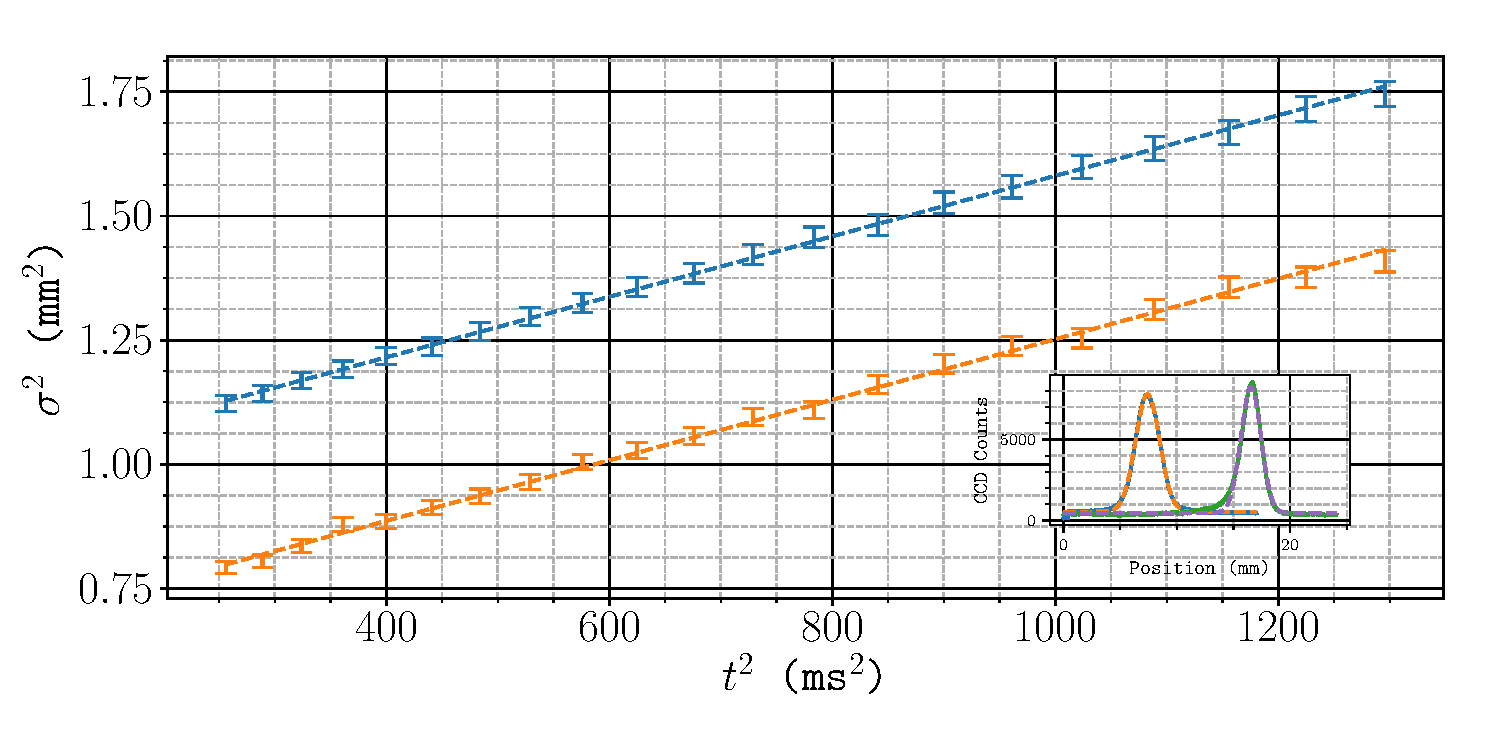
\includegraphics[width=0.8\textwidth]{temperature_launch}
    \caption[Temperature measurement using ballistic expansion]{Atom cloud temperature using a ballistic expansion measurement. After molasses, the cloud is left to expand in the dark and in a region of close to zero magnetic field. A least-squares linear fit of \(\sigma(t)^2\) is used to estimate the temperature using~\EquationRef{eg:expansion_width}. The inset shows a typical density profile from a single image, obtained by integrating the signal from a CCD camera along the two axes of the the sensor. The gradient from the fits for the horizontal (blue) and vertical (orange) axes are  \(T_x = \sivalue{6.38 \pm0.15}{\micro\kelvin}\) and \(T_y = \sivalue{6.38\pm0.12}{\micro\kelvin}\).}
    \label{fig:molasses_temperature}
\end{figure}

\subsubsection{Measuring the Launch Trajectory}
The same method used to measure the temperature of the cloud can also be used to measure the position of the centre-of-mass. In this case, the quantity of interest is \(\langle x(t)\rangle\). Since the cloud is in free-fall, the trajectory for the centre-of-mass is then given by the well-known equation-of-motion for a particle moving under constant acceleration
\begin{equation}
    \langle x(t) \rangle = \langle x(0) \rangle + v_x t + \frac{1}{2} a_x t^2
    \label{eq:position_free}
\end{equation}
where \(v_i\) is the initial velocity along the given axis and \(a_i\) is the acceleration.
\par\noindent
To launch the atoms both vertically and horizontally (along the axis parallel with the Raman light), the \((z_+, z_-)\) \acp{aoms} were ramped so that the relative frequency difference between each beam was \(2\times\)\sivalue{320}{\kilo\hertz} and the \(x\) and \(y\) \ac{aom} frequencies were ramped to give a frequency difference of \(2\times \sivalue{75}{\kilo\hertz}\) between the horizontal \ac{mot} beams. \FigureRef{fig:molasses_launch} is a plot of the measured centre-of-mass position along the horizontal and vertical camera axes over time. A linear least-squares fit to~\EquationRef{eq:position_free} gives a vertical launch quantities of \(v_v = \sivalue{25.0\pm0.35}{\centi\meter\per\second}\) and \(a_v = \sivalue{-9.40\pm0.075}{\metre\per\second\squared}\) and \(v_h = \sivalue{7.39\pm0.21}{\centi\meter\per\second}\) and \(a_h = \sivalue{-0.31\pm0.052}{\metre\per\second\squared}\) along the horizontal axis. 
\begin{figure}
    \centering
    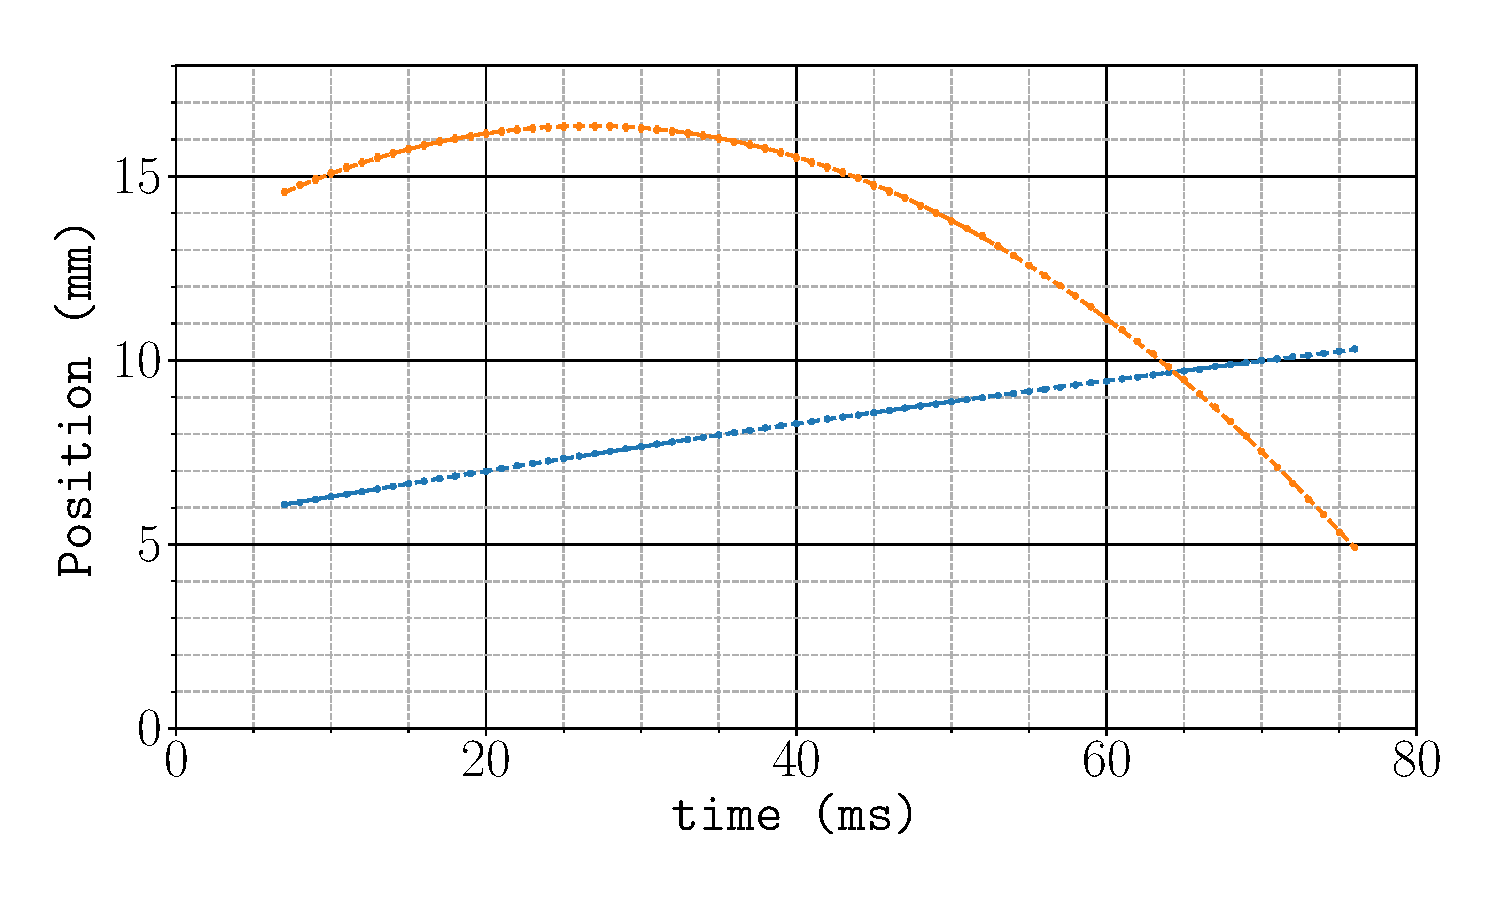
\includegraphics[width=0.8\textwidth]{molasses_position}
    \caption[Atom cloud centre-of-mass over time]{Measured centre-of-mass position over time. The horiztonal component of the position is shown in blue and the vertical in orange. Each trajectory is fit to~\EquationRef{eq:position_free} to estimate the launch velocity. The best-fit values are \(v_v = \sivalue{25.0\pm0.35}{\centi\meter\per\second}\) and \(a_v = \sivalue{-9.40\pm0.075}{\metre\per\second\squared}\) along the vertical axis and \(v_h = \sivalue{7.39\pm0.21}{\centi\meter\per\second}\) and \(a_h = \sivalue{-0.31\pm0.052}{\metre\per\second\squared}\) along the horizontal.}
    \label{fig:molasses_position}
\end{figure}
\par\noindent
When compared to the expected velocities from the detunings, \(v^{(l)}_v = \sivalue{24.96}{\centi\metre\per\second}\) and  \(v^{(l)}_h = \sivalue{5.85}{\centi\metre\per\second}\), the measured horizontal velocity is far greater than expected. This can be explained by a residual magnetic field, that is not cancelled using the bias coils. In the presence of a magnetic field, atoms cooled in an optical molasses are decelerated to a velocity at which the Zeeman shift is cancelled by the Doppler shift. This \ac{vsr} depends on the orientation of the magnetic field to the polarisation of the light. In a one-dimensional optical molasses, a {vsr} occurs at \(v_\text{res}^{(1)} = - \mu_B g_F B/\hbar k\) when the magnetic field is aligned with the wave-vector of the light \cite{VanderStraten1993}. When the field is aligned at an arbitrary angle an additional resonance at \(v_\text{res}^{(2)} = - \mu_B g_F B/2\hbar k\) is present, due to additional \(\left(\sigma^{\pm}-\pi\right)\) transitions~\cite{Chang2002}. A residual field along the Raman axis of \sivalue{20}{\milli\gauss} would shift the \ac{vsr} along \(\vec{x}\) and \(\vec{y}\) by \sivalue{1.09}{\centi\metre\per\second} corresponding to a velocity of \sivalue{1.54}{\centi\metre\per\second} along the Raman axis. 

\section{State Preparation}\label{sec:state_prep}
After the atoms have been cooled in an optical molasses, the population will mostly be distributed across the \(\ket{F=2}\) level, along with a small fraction distributed across the \(\ket{F=1}\) level. The Raman transition only couples the \(\ket{1,0}\) and \(\ket{2,0}\) states, so atoms in the other hyperfine ground states cannot participate in the interferometer. In fact, since the individual Zeeman sub-levels are not resolved during detection, these background atoms result in a loss of fringe visibility. One way to overcome this is to apply a pulse of light resonant with the \trans{2}{3} transition to push the non-participating atoms out of the interferometer detection region. Of course, this must be done after applying a Raman pulse to transfer an ensemble of atoms from \(\ket{2,0}\) into \(\ket{1,0}\). In this simple scheme a large fraction of the atoms are removed, which is undesirable since measurements of a low number of atoms are inherently more uncertain due to shot number fluctuations. 
\par\noindent
The following section discusses a method of preparing the atoms to increase the population in the \(\ket{1,0}\) ground state. An overview of the scheme is given in~\SectionRef{subsec:prep_schemes}. This is followed by a discussion of the initial steps which optically pump atoms into the \(\ket{1,0}\) state in~\SectionRef{subsec:optical_pumping}. A description of the microwave pulse used to drive atoms into the \(\ket{F=2}\) level is given in~\SectionRef{subsex:microwaves}. This section concludes with the method used to blow away the atoms which do not contribute to the interferometer in~\SectionRef{subsec:blow_away}. A key step which has been omitted is the velocity-selective Raman pulse. This is described in more detail later, in~\SectionRef{subsec:raman_velocity_select}
\subsection{Schemes for Preparation}\label{subsec:prep_schemes}
The scheme used to prepare atoms in the \(\ket{1,0}\) state is the following:
\begin{enumerate}
    \item Light resonant with the \trans{2}{2} transition pumps atoms into the \(\ket{F=1}\) level
    \item Light resonant with the \trans{1}{0} transition drives (\(\sigma^{\pm}\)) transtions to pump atoms into the \(\ket{1,0}\) dark state
    \item A microwave $\pi$-pulse transfers atoms to \(\ket{2,0}\)
    \item A Raman $\pi$-pulse transfers atoms with a narrow velocity spread back to \(\ket{1,0}\)
    \item The atoms which remain in \(\ket{F=2}\) are blown away
\end{enumerate}
A diagram of the population of each hyperfine ground state and the laser frequencies used to drive these transitions is given in~\FigureRef{fig:state_prep}. With the exception of step 4, the light is provided by the \Muquans laser using the \ac{mot} collimators aligned to the vertical \(\vec{z}\) axis. The frequency of the cooling laser and the repump sideband are set so that the relevant transitions for steps 1 and 2 are addressed. As the \(\ket{F=1}\) light is a sideband of the \(\ket{F=2}\) light, it is not possible to blow away atoms in \(\ket{F=1}\) without also blowing away atoms in \(\ket{F=2}\). This problem is overcome by using microwave pulses to drive atoms up to \(\ket{F=2}\) before velocity selection.
\par\noindent
A timing diagram of the state preparation sequence is shown in~\FigureRef{fig:state_selection_timing}, which indicates the duration for which each optical or microwave pulse is applied, as well as the direction of the applied magnetic field. The field is switched slowly over \sivalue{2}{\milli\second} (which is omitted from the diagram) to preserve the spin state of each atom. 
\begin{figure}
    \centering
    %\def\svgwidth{0.8\textwidth}
    \fontsize{16pt}{16pt}
    \resizebox{0.8\textwidth}{!}{\input{state_selection.pdf_tex}}
    \caption[State preparation pulse sequence]{Sequence of optical and microwave pulses used to prepare an ensmble of atoms in \(\ket{1,0}\). The red arrows indicate optical transitions to and from \(\ket{F=2}\) and equivalently for the blue arrows and \(\ket{F=1}\). A residual population in the \(\ket{1,\pm 1}\) states is present, which contributes to a background during the interferometer.}
    \label{fig:state_prep}
\end{figure}
\begin{figure}
    \centering
    %\def\svgwidth{0.5\textwidth}
    \fontsize{14pt}{14pt}
    \resizebox{0.6\textwidth}{!}{\input{state_selection_timing.pdf_tex}}
    \caption[State selection timing schematic]{Timing diagram for state selection sequence. The durations labelled are indicative of the time required to drive the atoms into the desired state at each step. After the \trans{1}{0} pumping, the magnetic field is re-oriented along the Raman axis \(\vec{r}\). The \sivalue{2}{\milli\second} field switching time has been omitted.}
    \label{fig:state_selection_timing}
\end{figure}
\subsection{Optically Pumping the Atoms}\label{subsec:optical_pumping}
\subsubsection{Driving the \trans{2}{2} transition}
After the molasses, the frequency of cooling light is \sivalue{150}{\mega\hertz} below the \trans{2}{3} transition. This can off-resonantly excite an atom to the \(\ket{F'=2}\) excited level, but the small scattering rate means that on average, an atom will need to scatter many photons before it is pumped into the \(\ket{F=1}\) level. Therefore, to minimise the heating during this pumping process, the frequency of the cooling light is resonant with the \trans{2}{2} transition.
\par\noindent
\FigureRef{fig:step1_pumping} shows the population in the two hyperfine ground states as the duration of the \trans{2}{2} light is increased. The rate at which atoms are pumped into \(\ket{F=1}\) increases with the strength of the applied magnetic field. At zero field, there exists a dark state which is a coherent superposition of the \(\ket{2,m_F}\) states~\cite{Berkeland2002}. Applying a magnetic field lifts the degeneracy between the Zeeman sub-levels so that this dark state is no longer stationary. The evolution rate of this dark state, and hence pumping rate, increases with an increasing Zeeman shift. At a field strength of \sivalue{3}{\gauss}, the atoms can be pumped into \(\ket{F=1}\) in less than \sivalue{5}{\micro\second}.
\begin{figure}
    \centering
    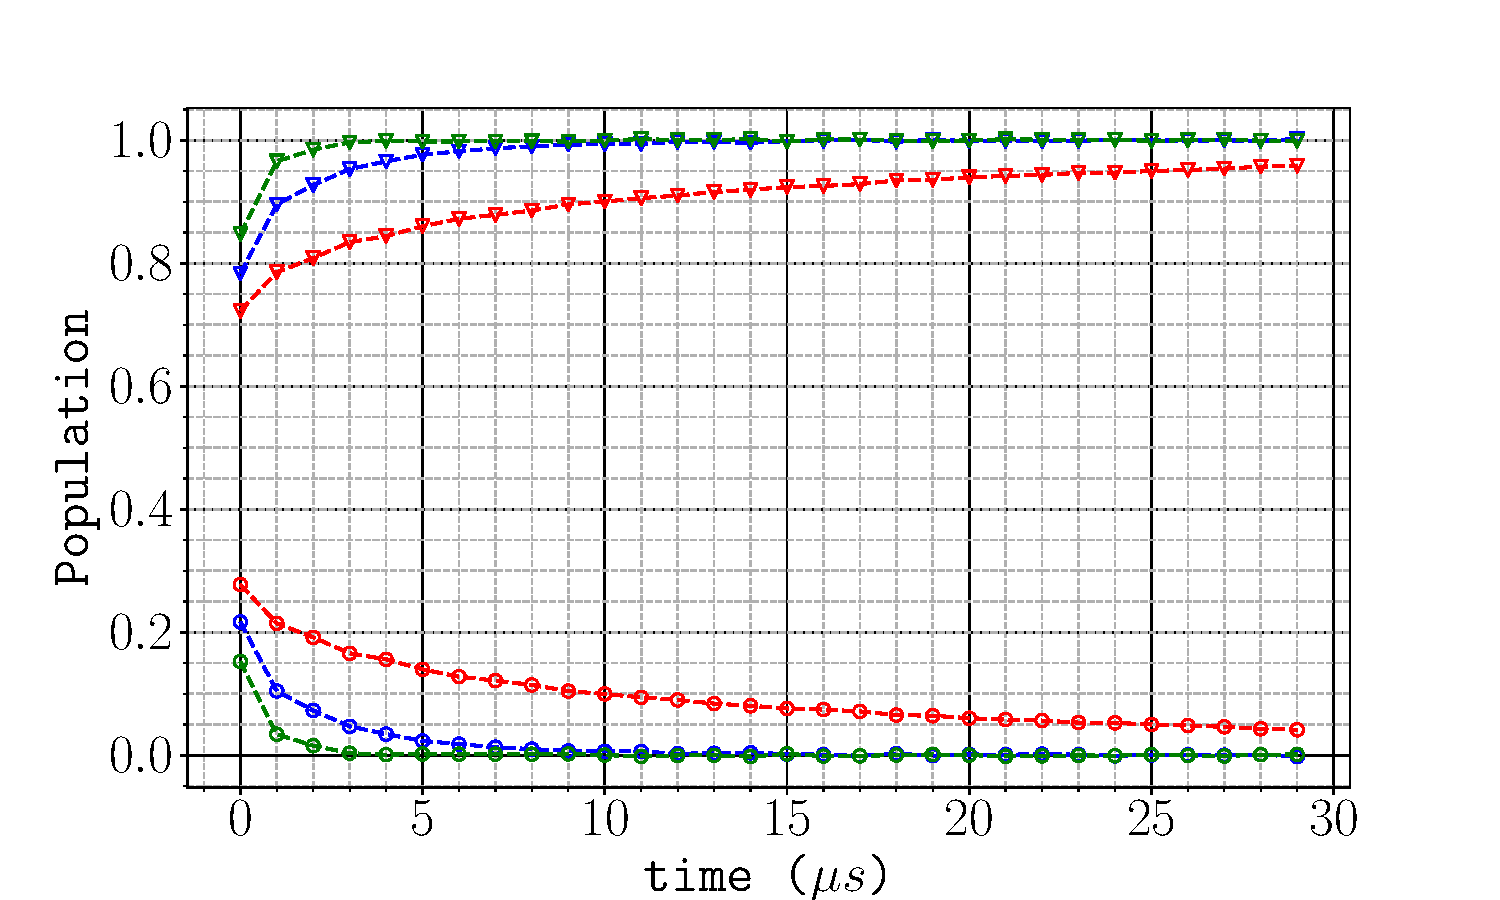
\includegraphics[width=0.5\textwidth]{step1_pumping}
    \caption[Ground state distribution during \trans{2}{2} pumping]{Population across the two hyperfine ground states after \trans{2}{2} pumping under various magnetic field strengths. The $\smalltriangledown$ ($\circ$) markers indicate the population in $\ket{F=2}$ ($\ket{F=1})$. The red, blue and green series correspond to field strengths of \sivalue{-0.16}{\gauss}, \sivalue{1.67}{\gauss}, and \sivalue{3}{\gauss}, respectively.}
    \label{fig:step1_pumping}
\end{figure}
\subsubsection{Driving the \trans{1}{0} transition}
After this first pumping step, the atoms are distributed across the Zeeman sub-levels in \(\ket{F=1}\). The next pulse of light is used to increase the population in \(\ket{1,0}\) by driving \trans{1}{0} transitions. During this time, the \trans{2}{2} light remains on which helps to prevent atoms from populating the \(\ket{F=2}\) level through off-resonant \trans{1}{1} excitations. The magnetic field present means that the circularly-polarised \(\vec{z}\) \ac{mot} beams only drive \(\sigma^{\pm}\) transitions, so the \(\ket{1,0}\) state is in principle a dark state. 
\par\noindent
The distribution of atoms across the Zeeman sublevels was measured using a microwave pulse to drive atoms into the \(\ket{F=2}\) level, which is described in~\SectionRef{subsec:microwaves}. For each \(\pi\) microwave transition, the frequency of the microwave field was varied to find the resonant frequency. The resulting spectra for \(m_F = -1\)  and \(m_F = 0\) are shown in~\FigureRef{fig:step2_microwave_spec}, both with and without applying light to pump into the \(\ket{1,0}\) state.  The 0 \(\rightarrow\) 0 clock transition is detuned from the hyperfine splitting frequency due to the applied magnetic field, giving a second-order Zeeman shift of \sivalue{515}{\hertz\per\gauss\squared}. The measured shift of \sivalue{5.6}{\kilo\hertz} corresponds to a field strength of \sivalue{3.3}{\gauss}.
\begin{figure}
    \centering
    \def\svgwidth{\columnwidth}
    \subfloat[][]{\scalebox{0.3}{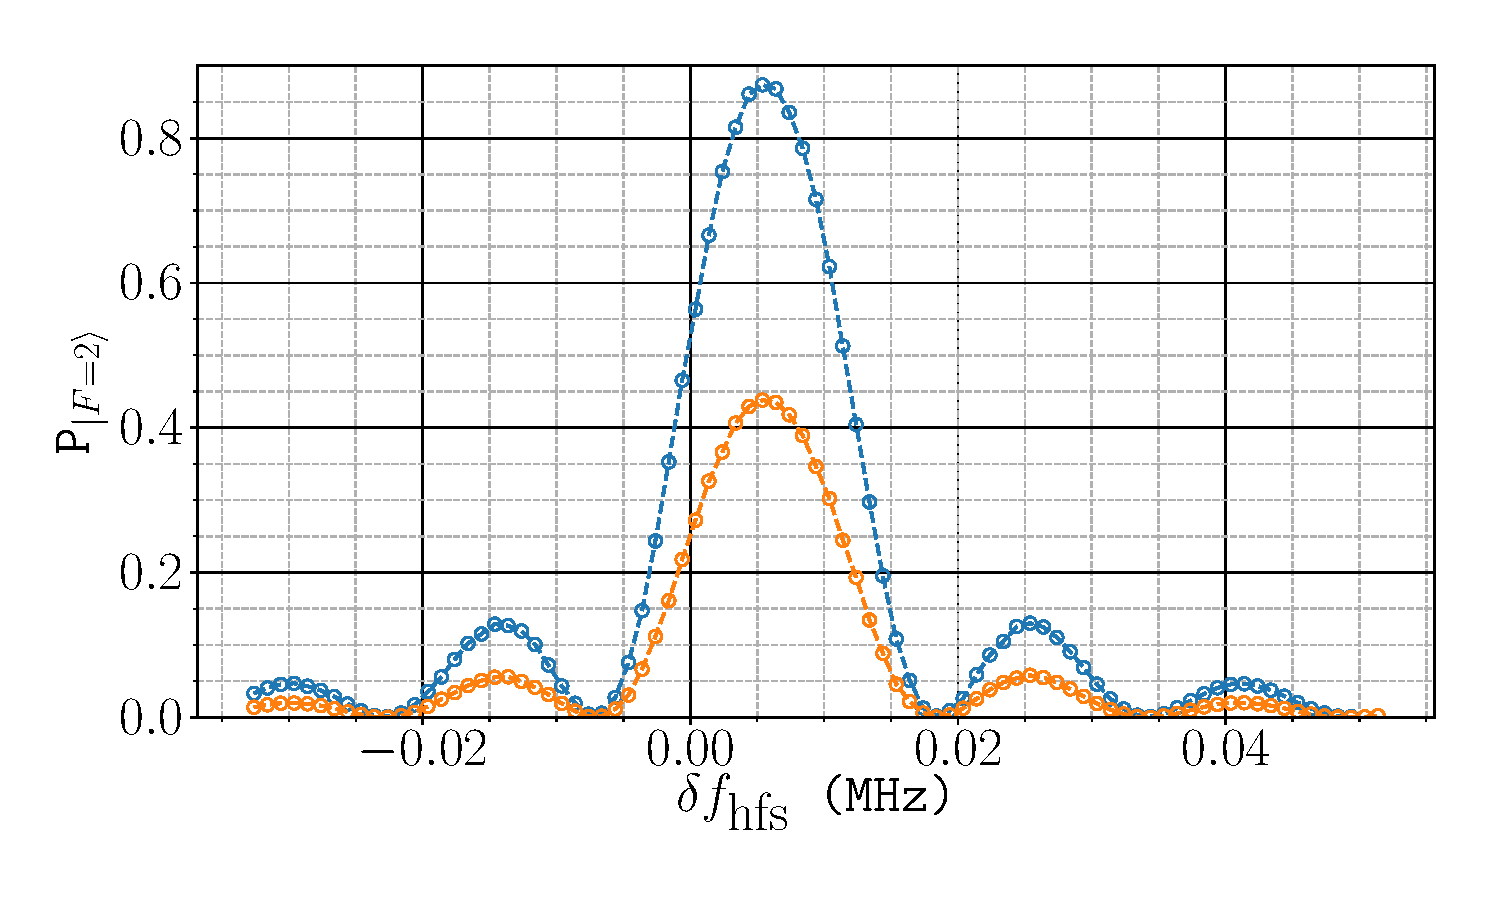
\includegraphics{step2_mf0}}\label{fig:step2_mf0}}
    \subfloat[][]{\scalebox{0.3}{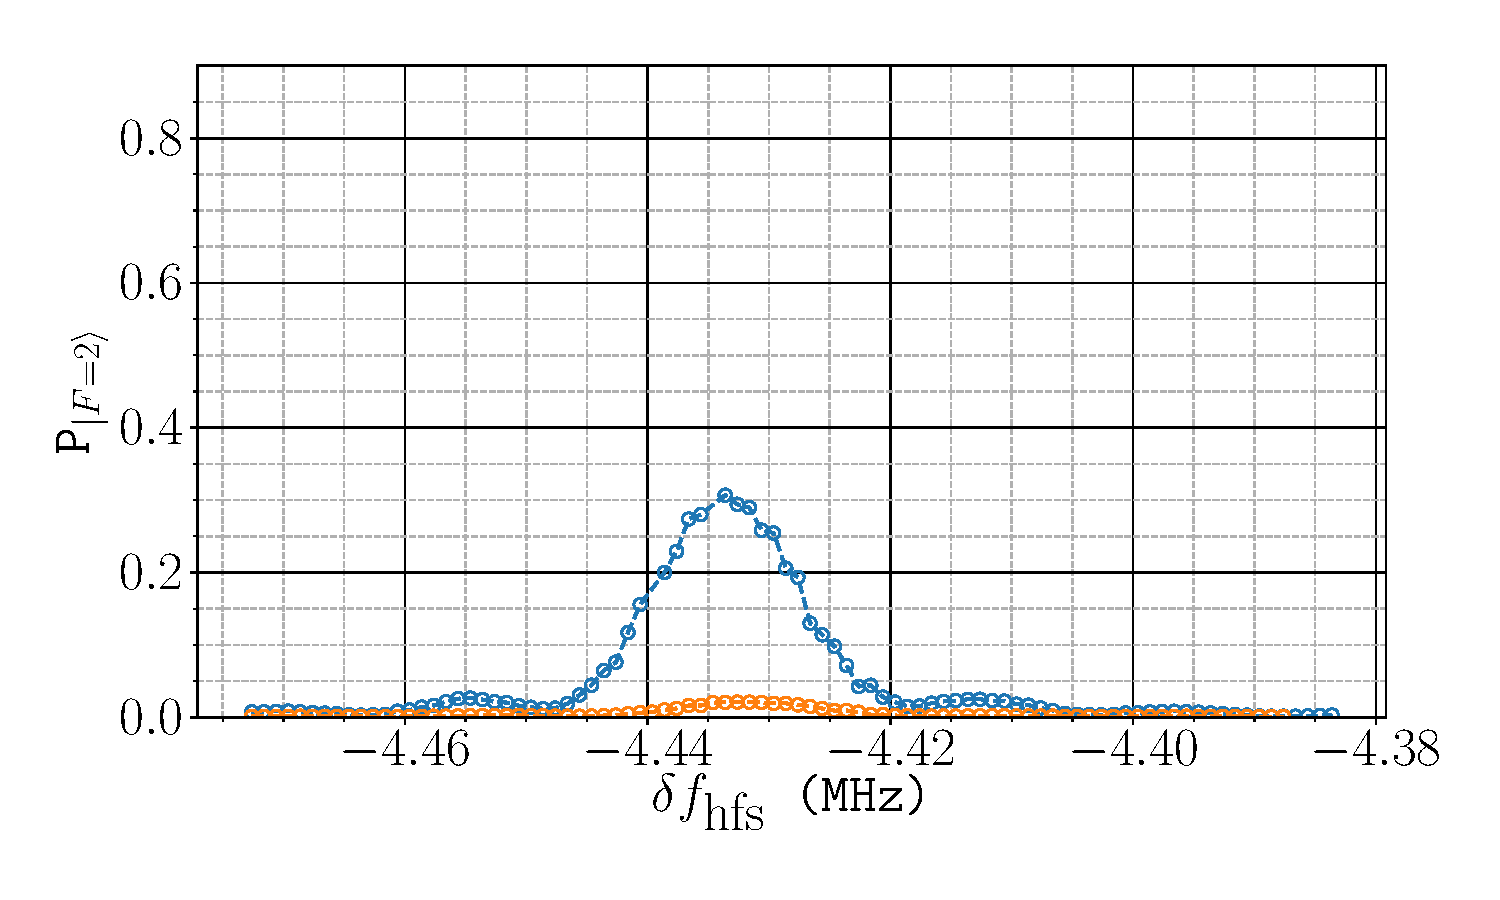
\includegraphics{step2_mf1}}\label{fig:step2_mf1}}
    \caption[\(m_F\) populations before and after \trans{1}{0} pumping]{Population of atoms in (a) \(\ket{1,0}\) and (b) \(\ket{1,-1}\), measured by applying a \sivalue{68}{\micro\second} microwave pulse to drive atoms into the \(\ket{F=2}\) level. The orange and blue points indicate the measured populations with and without \trans{1}{0} pumping. The microwave frequency is plotted as a detuning from the hyperfine splitting frequency \(f_\text{hfs}\).}
    \label{fig:step2_microwave_spec}
\end{figure} 
\par\noindent
A plot of the population in each Zeeman sub-level for increasing pumping times is given in~\FigureRef{fig:step2_pumping}. In this instance, the optical pumping does not completely deplete the population from the \(m_F = \pm 1\) sub-levels. After pumping for \sivalue{30}{\micro\second}, approximately 5\% of the population remains in the \(m_F = \pm 1\) sub-levels. The \(\ket{1,0}\) state can only be excited to \(\ket{F'=0}\) by \(\pi\)-polarised light, which suggests that the magnetic field is mis-aligned with the \(\vec{z}\) \ac{mot} beams. The effect of these background atoms on the measured interferometer signal is discussed later, in~\SectionRef{subsec:phase_measurement}.
\begin{figure}
    \centering
    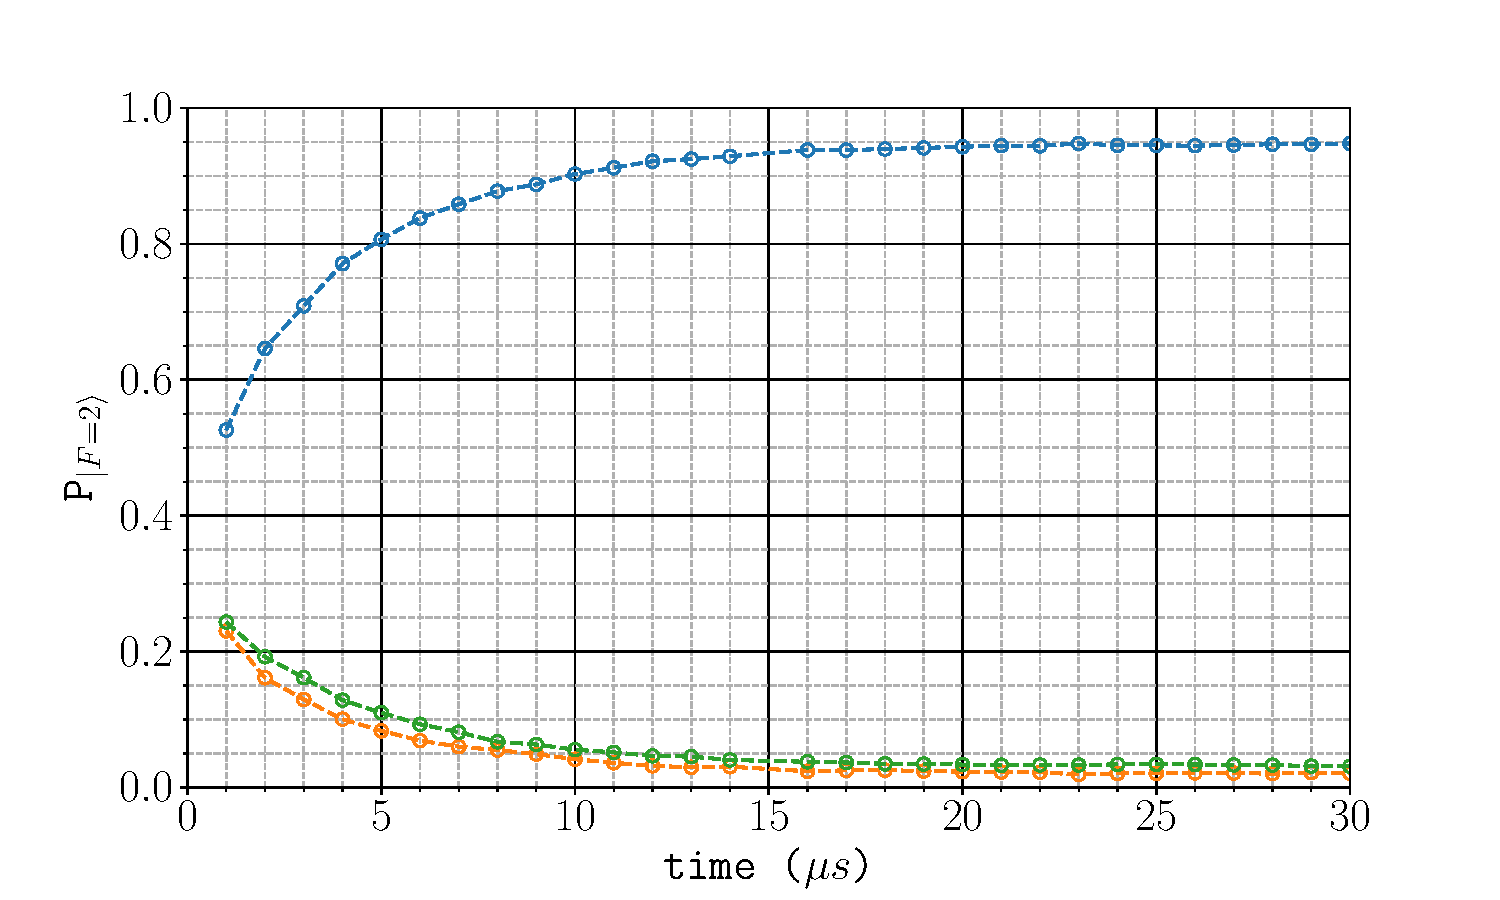
\includegraphics[width=0.8\textwidth]{step2_pumping}
    \caption[\(\ket{1,m_F}\) populations for increasing \trans{1}{0} pumping time.]{Population in each Zeeman sub-level as the \trans{1}{0} pumping time is increased. The \(m_F = 0, -1, +1\) populations are shown in blue, orange and green, respectively. After \sivalue{30}{\micro\second}, approximately 5\% of the population remains in the \(m_F = \pm 1\) sub-levels.}
    \label{fig:step2_pumping}
\end{figure}
\subsection{Including Microwave Transitions}\label{subsec:microwaves}
Without a dedicated laser to drive transitions from the \(\ket{F=1}\) level, it was necessary to implement a scheme to use light resonant with the \(\ket{F=2}\) level to remove background atoms. Therefore, we included a system for driving microwave frequency transitions from \(\ket{1,0}\) to \(\ket{2,0}\).
\subsubsection{Microwave Generation}
A diagram of the setup for this is shown in~\FigureRef{fig:microwave_setup}. The microwave radiation is generated using a \textit{Wind-Freak} synthesiser to output a microwave field oscillating at a frequency close to the hyperfine splitting frequency, \(f_\text{hfs} = \sivalue{6.83846}{\giga\hertz}\). This is amplified by \textit{MiniCircuits MCL ZRON-8G+} amplifier and directed into the chamber using a \textit{Pasternack PE9859/SF-10} microwave horn, which produces a linearly-polarised microwave field. The horn was aligned to the chamber at the position which maximised the population of atoms in the \(\ket{2,0}\) state. The synthesiser is clocked using a stable \sivalue{100}{\mega\hertz} signal from the \Muquans laser. When the synthesiser was clocked using its internal \sivalue{27}{\mega\hertz} reference clock, this produced a noticeable jitter in the output frequency, which led to a significant shot-to-shot fluctuation in the \(\ket{2,0}\) population.
\begin{figure}
    \centering
    \resizebox{0.5\textwidth}{!}{\input{microwave_setup.pdf_tex}}
    \caption[Setup for Microwaves]{Schematic diagram of the microwave assembly. The frequency close to the hyperfine splitting frequency is generated by a \textit{Wind-Freak} synthesiser. A \sivalue{100}{\mega\hertz} clock signal acts as a stable reference frequency for the synthesiser. The generated microwave power is amplified twice, first by a low-power \textit{Mini-Circuits} amplifier, then by a microwave horn, which produces a highly directional, linearly polarised wave. The output is controlled by a digital signal, both at the synthesiser and at a bi-directional microwave switch. The second port of this is blocked with a \sivalue{50}{\ohm} terminator to prevent reflections. }
    \label{fig:microwave_setup}
\end{figure}
\subsubsection{Pulse Characterisation}
\FigureRef{fig:mw_rabi} shows a measurement of the population in the \(\ket{F=2}\) level for increasing durations duration of the applied microwave pulse. Rabi oscillations between the \(\ket{1,0}\) and \(\ket{2,0}\) states are clearly present. The loss of coherence between the states can be explained by an inhomogeneous driving field. Once inside the chamber, the microwaves reflect and scatter off the interior surfaces which results in a spatially-dependent Rabi frequency. This also leads to a depolarisation of the field, as \(\sigma^{\pm}\) transitions were also observed. Initially, around \(85\%\) of the population was driven into \(\ket{F=2}\) using a microwave pulse of \sivalue{100}{\micro\second}. After improving the alignment of the magnetic field during the microwave pulse, this fraction increased to \(97\%\) - the remaining 3\% being distributed across the \(m_F = \pm 1\) states.

\begin{figure}
    \centering
    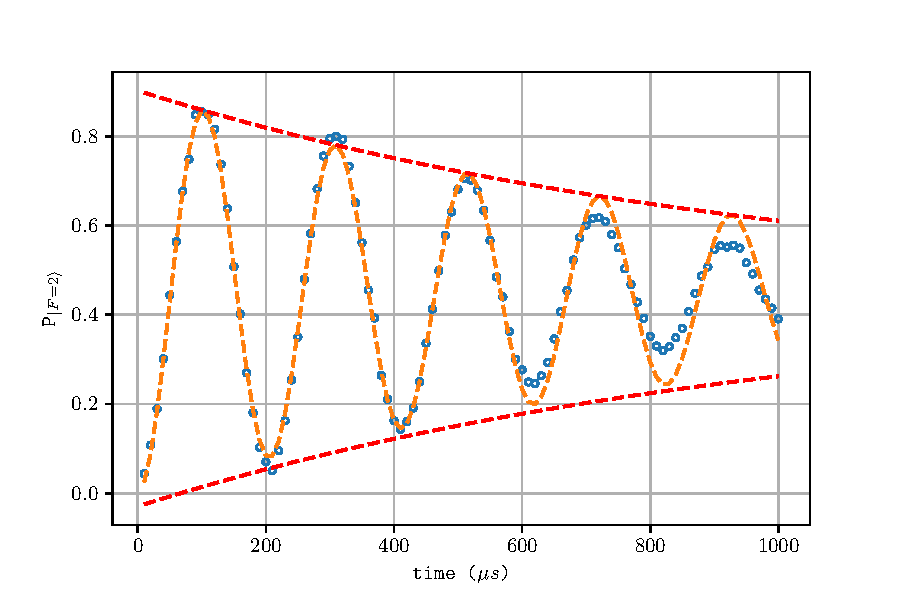
\includegraphics[width=0.5\textwidth]{mw_rabi}
    \caption[Microwave Rabi oscillation between \(\ket{1,0}\) and \(\ket{2,0}\)]{Damped Rabi oscillation between \(\ket{1,0}\) and \(\ket{2,0}\) using a microwave pulse of varying length. At longer pulse times, there is a loss of coherence due to a depahasing between the two states. The red dashed line is an envelope is a fit to a decaying exponential with a characteristic time of \(\tau = \sivalue{1016}{\micro\second}\).}
    \label{fig:mw_rabi}
\end{figure}
\par\noindent
\FigureRef{fig:microwave_transitions} shows a spectrum obtained by varying the frequency of the microwave pulse. This shows the presence of \(\Delta m = \pm 1 \) transitions from \(\ket{1,0}\), as well as the fact that the population in \(\ket{1,m_F=\pm 1}\) decreases after the \trans{1}{0} pumping step is applied. The linewidth of the microwave transition is much narrower than the Zeeman splitting, so only the clock transition is driven when a pulse with a frequency close to \(f_\text{hfs}\) is applied.
\begin{figure}
    \centering
    \def\svgwidth{\columnwidth}
    \subfloat[][]{\scalebox{0.7}{\input{microwave_spectrum.pdf_tex}}\label{fig:microwave_spectrum}}
    \subfloat[][]{\scalebox{0.3}{\raisebox{3ex}{\input{microwave_transitions.pdf_tex}}}}
    \caption[Microwave transition spectrum]{Microwave transition spectrum before (blue) and after (orange) \trans{1}{0} pumping. (b) shows the transitions addressed as the microwave frequency is varied. Dashed and lines indicate \(\Delta m = \pm 1\) transitions and solid lines indicate \(\Delta m = 0\). In order of increasing frequency, the transitions in (a) are highlighted in: a) red, b) blue, c) green, d) orange and e) purple.} 
    \label{fig:microwave_data}'
\end{figure}

\subsection{Blow-Away}\label{subsec:blow_away}
After the atoms populate \(\ket{2,0}\), a velocity-selective Raman \(\pi\)-pulse is applied to transfer a fraction of those back into \(\ket{1,0}\). This step is discussed in detail in~\SectionRef{subsec:raman_velocity_select}. For now, it suffices to say that a Raman pulse transfers 4\% \textbf{Check this!} the atoms back to \(\ket{1,0}\). The remaining need to be removed, otherwise they contribute to a large background signal. \par\noindent
The final pulse during the state preparation sequence is used to push these non-contributing atoms out of the interferometer region. A single \ac{mot} beam is used so that there is a net momentum transfer to the atoms as they absorb light and fluoresce. The frequency of this blow-away beam is detuned from the \trans{2}{3} transition by \sivalue{-3}{\mega\hertz}, which is the same frequency used for detection (see~\SectionRef{sec:atom_detection}). A pulse of \sivalue{50}{\micro\second} is enough to remove all atoms in \(\ket{F=2}\). 

% \subsection{Residual \(m_F = \pm 1\) atoms} \label{subsec:residual_atoms}
% After preparing an ensemble atoms in \(\ket{1,0}\) with a narrow velocity spread and removing those out in \(\ket{F=2}\) which are not resonant with the interferometer pulses, there is still a fraction of atoms in \(\ket{1,\pm 1}\) which will be detected and contribute to a background signal. It is worth highlighting how fluctuations in this background affects the sensitivity of the interferometer to accelerations. Since they are not driven by the Raman transition, they remain in \(\ket{F=1}\). If the number of atoms detected in \(\ket{F=1}\) has a contribution from background atoms, i.e \(N_1 = N_\text{bg}+N_1^{(\phi)}\), then the probability of detecting an atom in \(\ket{F=1}\) is given by
% \begin{equation}
%     P_{\ket{F=1}} = P_0 + \frac{C}{2}\sin{\Delta \phi}^2
% \end{equation}
% where \(P_0 = N_\text{bg}/\left(N_1+N_2\right)\) is the proportion of background atoms out of the total number of atoms.

\subsection{Conclusion}
This chapter has presented the stages of the experiment which are used to prepare an ensemble of atoms for interferometry. This requires cooling the atoms to limit the thermal expansion of the cloud during interferometry. The atoms are also launched using a moving molasses so that only one pair of beams is resonant with the Raman transition. Finally, we then apply a sequence of optical and microwave pulses, to increase the population of atoms in \(\ket{1,0}\). A velocity-selective Raman pulse with a narorow linewidth is used to make the velocity spread along the Raman axis much smaller than the Doppler width. Aside from some residual population in \(\ket{1,\pm 1}\), the remaining atoms are removed using a pulse of light close to resonance with the \trans{2}{3} transition. This results in an ensemble of which around \(40\%\) of the population contributes to the interferometer signal.


    \chapter{Acceleration-Sensitive Interference}\label{chap:atom_int}

\section{Chapter Outline}
This chapter describes the aspects of the project aimed at observing
matter-wave interference in \ac{rb87} and its subsequent
characterisation. The laser system used to drive the necessary Raman
transitions is presented in~\SectionRef{sec:msquared_laser}. This is
followed by a discussion of the methods used to detect the population
in each internal state in~\SectionRef{sec:atom_detection}. The Raman
transition spectrum and
dynamics of the atoms during each Raman pulse are discussed
in~\SectionRef{sec:atomint_rabiosc}. This chapter continues
with an overview of indentified sources of noise and their impact on
the interferometer's sensitivity to accelerations
in~\SectionRef{sec:atomint_sensitivity}. Finally, a presentation of observed
interference and an analysis of its sensitivity to accelerations is
given in~\SectionRef{sec:atomint_accelerations}.
\section{The M-Squared Laser System}\label{sec:msquared_laser} 
  This section describes the laser system manufactured by \textit{M-Squared
  Lasers}, which is used to drive Raman transitions. 
  A \ac{pll} controls the phase difference of two Ti:Sapphire lasers
  by comparing the beat note with a stable local oscillator\nocite{Lautier2014b}\nocite{Marino2008}. An overview of the laser
  system can be found in~\SectionRef{subsec:msquared_overview}, which includes
  the techniques used to externally communicate with the laser's ICE-BLOC
  control modules. The control of the frequency and phase-lock is then described
  in~\SectionRef{subsec:msquared_control}. Finally, this section concludes
  in~\SectionRef{subsec:dcs_module} with a description of the DCS
  module which is used to control
  the amplitude, frequency and phase of the Raman laser beat-note
  during the experiment.
\subsection{Laser System Overview}
\label{subsec:msquared_overview} The Raman laser system contains two
SolsTiS lasers, each generating \sivalue{780}{\nm} light by pumping a Ti:Sapphire crystal housed inside a resonator.
The output light is frequency-stabilised using piezo-electric stacks to adjust
the resonator length~\cite{Drever1983}. A schematic diagram of this laser system is given
in~\FigureRef{fig:msquared_laser}. Each laser is pumped using a
\sivalue{12}{\W} \textit{Lighthouse Photonics} Sprout laser at
\sivalue{532}{\nm}. One SolsTiS acts as the master frequency locked
to an absorption feature in the saturated absorption spectrum of
\ac{rb87}. The second is slaved to this using a phase-locked loop to keep their
beat frequency constant. The two beams are mixed on a
\ac{pbs}, so that they are orthogonally polarised. Two \acp{aom} control the
output power. 
%A planned upgrade for this system will have multiple output ports
%for the Raman light, which will require independent control. 
\par\noindent 
The system contains 4 ICE-BLOC modules which implement various types of control. The
first two (one for each Solstis) are used to stabilise the output power of each
laser by feeding back to the corresponding Sprout laser. They are also used to
coarsely adjust the output frequency, which is measured using a
\textit{HighFinesse} wavemeter. The third is used for the \ac{pll}
and feeds-back onto the slave laser to control both the frequency and phase of
the optical beat-note between the two lasers. The final ICE-BLOC, referred to
as the DCS module, is used to control the lasers in real-time during the
experiment.  
\begin{figure}
	\centering \fontsize{10pt}{10pt}
	\resizebox{0.8\textwidth}{!}{\input{msquared_laser.pdf_tex}}
	\caption[M-Squared Laser System Schematic]{Schematic Diagram of the M-Squared
		laser system. Two SolsTiS lasers provide the two Raman frequencies, which
		are fibre coupled onto the orthogonal axes of a \ac{pm} fibre. Control of
		the power, frequency and phase as required to drive and control
    the Raman transitions is
		handled by the four ICE-BLOC modules indicated in blue. Further detail of
		this control is given in the text.} \label{fig:msquared_laser}
\end{figure}

\subsubsection{External ICE-BLOC Control}
The ICE-BLOC modules are able to communicate with each other using an Ethernet
hub. Another computer connected to this network is able to control them by
accessing a web page that each module hosts. These web pages control the ICE-BLOCs
by sending structured JSON messages. This graphical interface can be bypassed by
directly communicating these messages. This is done using MOTMaster so that
various parameters, such as the frequency and phase of the Raman beat-note, can
be automatically varied between experiment cycles. 
\subsection{Frequency and Phase Control}\label{subsec:msquared_control}

\subsubsection{Master Lock}
The frequency of the master laser is stabilised using saturated absorption
spectroscopy in a Rubidium vapour cell. Part of the beam is picked off and
modulated by an \ac{eom}. The positive frequency sideband is used to lock the
master laser to the 2,3 crossover feature. In effect, this means that the
modulation frequency of the \ac{eom} sets the one-photon detuning of the Raman
transition. The modulation frequency is set so that the master laser frequency
is \sivalue{1.13}{\giga\hertz} below the \trans{2}{3} transition. This
frequency is chosen because the light shift of the clock transition
vanishes there provided the two Raman beams have the right intensity
ratio as discussed in~\SectionRef{subsec:light_shift}. This ensures
that the resonant frequency is independent of variations in the
over-all intensity of the Raman beams.
\subsubsection{Frequency and Phase Lock} The optical beat-note between the two
lasers is measured using a fast photodiode. The signal from this is used in a
\ac{pll} to fix the relative phase between the two lasers. A frequency
divider halves the frequency of the signal before comparing it to a \ac{vco} of
around \sivalue{3.4}{\giga\hertz}. This creates an error signal which used to
control both the frequency and phase of the beat-note by feeding back to the
slave laser Solstis. The relative phase between the two lasers is adjusted using
an analogue phase shifter and the frequency difference is controlled by tuning
the \ac{vco} frequency. \par\noindent The beat-frequency of the Raman lasers can
be chirped by triggering a ramp of the control voltage to the \ac{vco}. For
chirp rates of lower than \sivalue{24}{\mega\hertz\per\second}, the phase-lock
is able to keep the beat-note phase-coherent during the chirp.  
\subsection{The DCS Module}\label{subsec:dcs_module} 
The DCS module is used to control the
output of the lasers during the experiment. It uses an on-board
\ac{dds} to
synthesise the \sivalue{80}{\mega\hertz} driving frequencies for each \ac{aom}.
The majority of the control is done using an \ac{fpga} that synthesises a timed
sequence of analogue and digital voltage waveforms. An example of a sequence
created using the DCS web interface is shown in~\FigureRef{fig:dcs_module}. The
sequence is segmented into individual steps and each channel can be separately
configured, much like the MOTMaster user interface. \par\noindent This module is
used to control the amplitude, frequency and phase of each Raman pulse. The
pulse amplitude is shaped using an analogue voltage to control the power of the
RF frequency. The voltage output has been calibrated so that the pulse can be shaped to
produce a square, Gaussian or Blackman amplitude envelope. A frequency
chirp of the beat-note is
optionally triggered by sending a digital pulse to the \ac{pll} ICE-BLOC.
\par\noindent The synthesiser can be configured to run continuously, or to wait
at a chosen timestep for an external trigger. It can also iterate through a set
number of parameters, such as timestep duration or phase shift by re-building
the sequence after each cycle.  
\begin{sidewaysfigure}[!htbp] 
  \centering
	\resizebox{1\textwidth}{!}{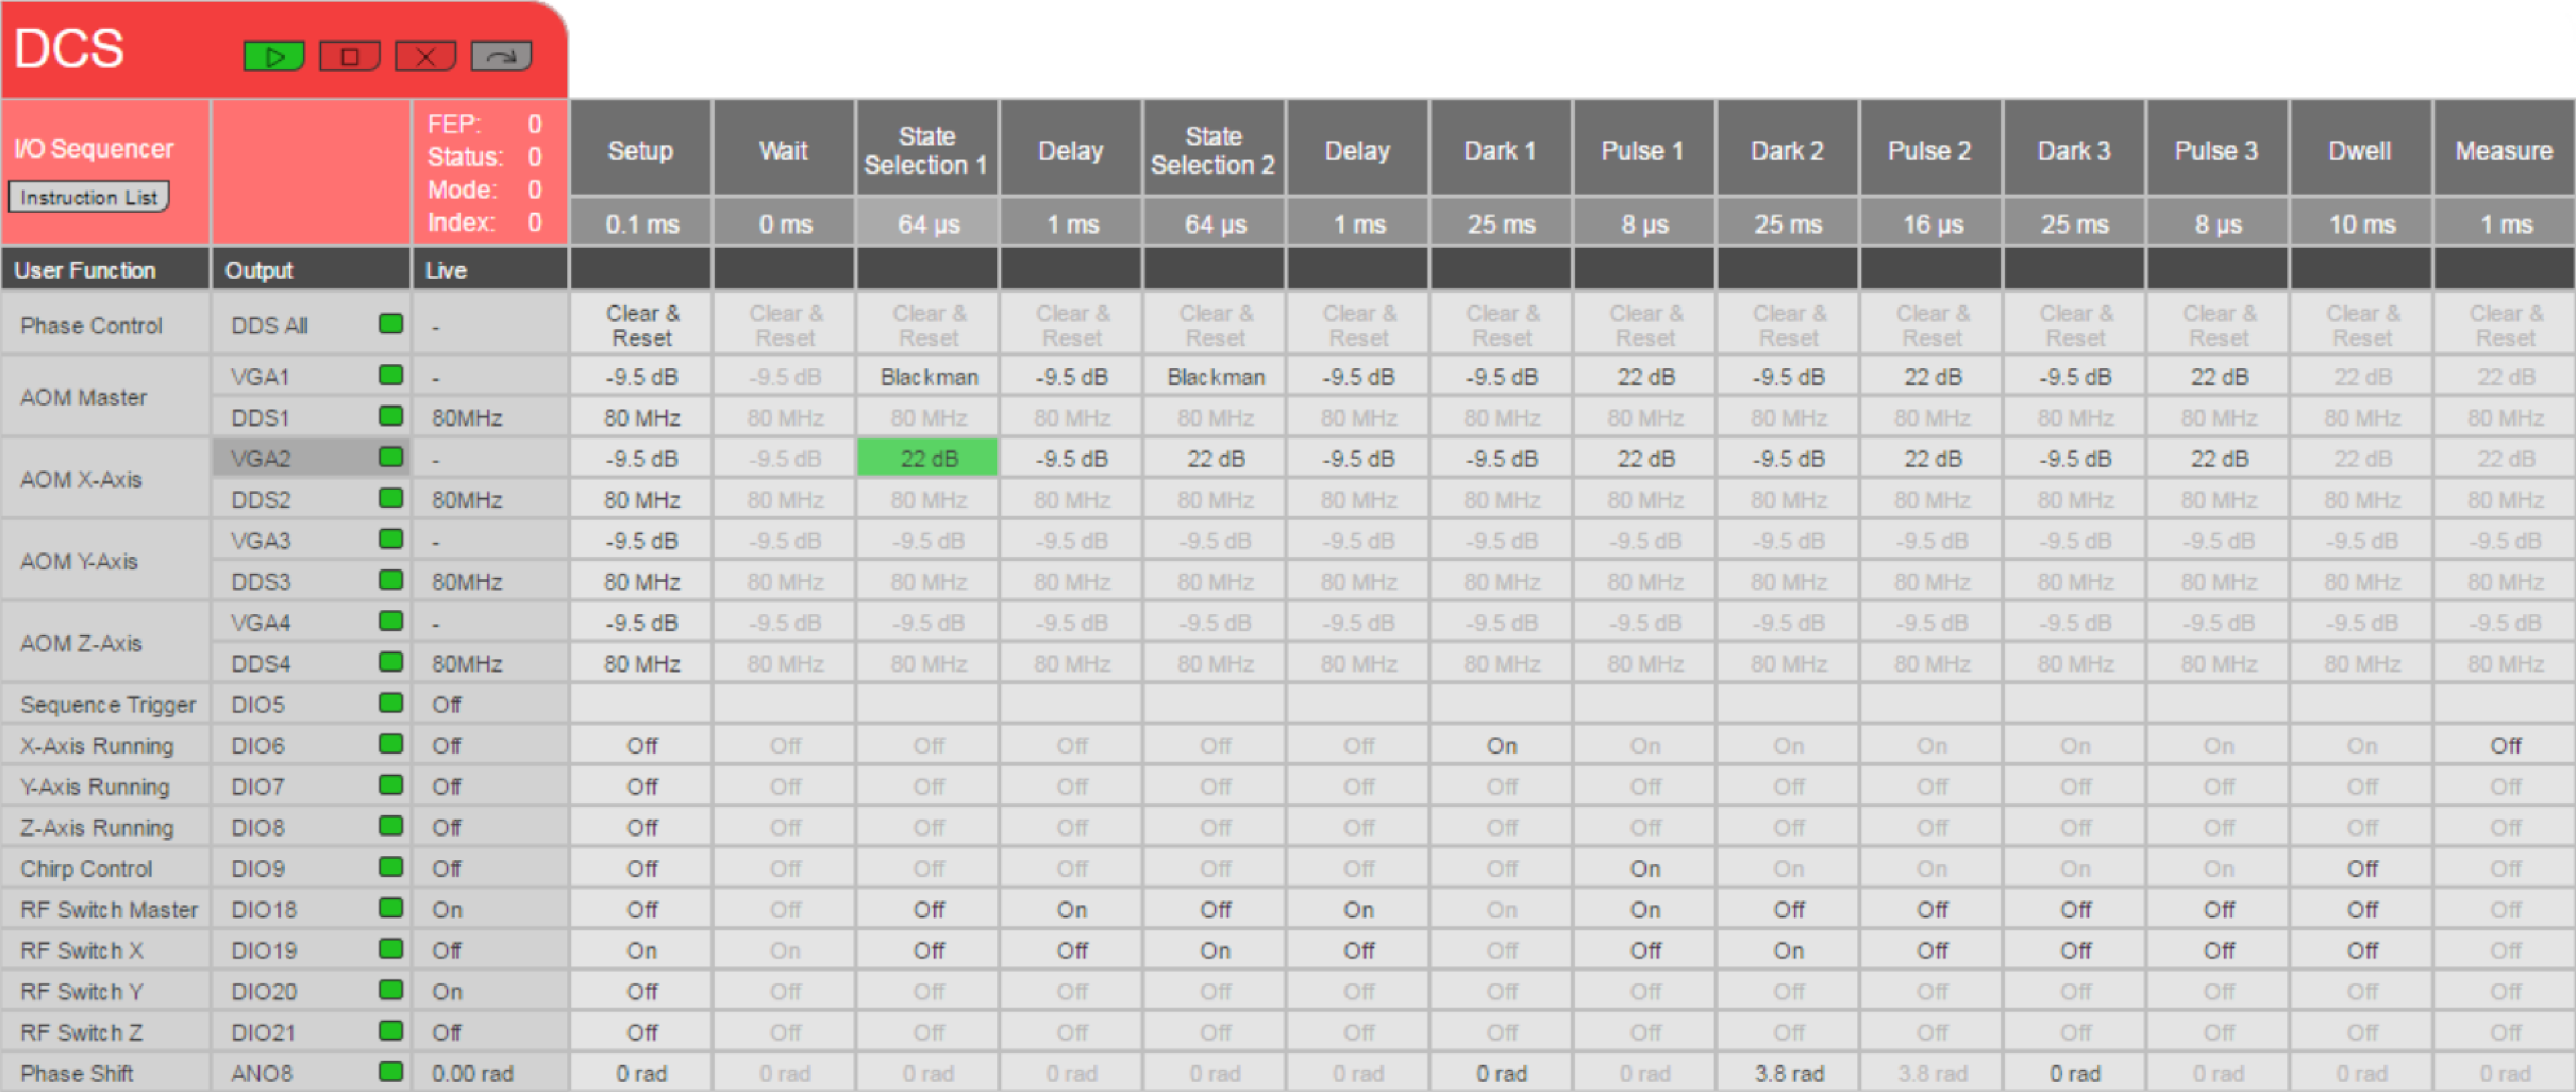
\includegraphics{dcs_module.pdf}}
	\caption[DCS Module User interface]{DCS module user interface. The sequence is
		synthesised from individual steps. The parameters of each Raman laser pulse
		can be configured independently.} 
  \label{fig:dcs_module} 
\end{sidewaysfigure}
\section{Atom Detection}\label{sec:atom_detection} 
This section describes the methods used to
measure the number of atoms in each hyperfine ground state and infer
the interferometer phase. It begins with a
presentation the optical setup used to collect fluorescent light on a
photodiode in~\SectionRef{subsec:optical_setup}.
The scheme used to detect the atoms by
driving \(\sigma^+\) transitions is then described in~\SectionRef{subsec:optical_setup}.
This concludes with a
discussion on converting the measured photodiode signals into atom
number and interferometer phase
in~\SectionRef{subsec:phase_measurement}.
\subsection{Optical Setup}\label{subsec:optical_setup}
Out aim in this device is to reach the standard quantum noise limit,
which comes from the quantum projection noise. Expressed as a
fractional accuracy this is given approximately by
$N^{-1/2}$~\cite{Bollinger1996}, where $N$ is the number of atoms detected.
The CCD used initially was not sensitive enough for this as there wass a
significant amount of noise in reading out the charge collected at each pixel.
Instead, a more sensitive photodiode is used to detect the atoms. With a
suitably high bandwidth, the readout time is much faster than the CCD as well,
so that the atoms can be detected well before they fall out of the field of
view. \par\noindent A diagram of the setup used to detect the atoms is given
in~\FigureRef{fig:photodiode_optics}. It is a triplet system which uses
lenses with focal lengths \sivalue{150}{\milli\metre},
\sivalue{75}{\milli\metre} and \sivalue{60}{\milli\metre}, with the
\sivalue{150}{\mm} lens closest to the atoms and the \sivalue{60}{\mm}
lens closest to the photodiode. A ray-tracing simulation of the optical
system indicates spherical aberrations on the image. This is caused by
the third lens, which was added to shorten the back focal length. The
front lens has a diameter of
\sivalue{50.4}{\milli\metre}, so the solid angle subtended by the
optics is \(4\pi \times\)\num{7.1e-3}\si{\steradian}.
\begin{figure}[!htbp] 
  \centering \fontsize{24pt}{24pt}
	\resizebox{0.7\textwidth}{!}{\input{photodiode_optics.pdf_tex}}
	\caption[Optical setup for Photodiode Detection]{Optical setup for photodiode
		detection. A triplet lens system focuses light from radiated from the atoms
		onto a photodiode. This is mounted using a translation stage to
  position the photodiode at the back focal point.}
  \label{fig:photodiode_optics}
\end{figure}

\subsubsection{Photodiode Calibration}
The photodiode used is a \textit{Femto LCA-S-400K-SI},
which has a trans-impedance amplifier with a bandwidth of \sivalue{400}{\kilo\hertz} and a photo-sensitive area
with a diameter of \sivalue{3}{\milli\metre}. The scaling factor from
incident optical power to output voltage was measured as \sivalue{1.84e6}{\volt\per\watt}. 
%\begin{figure}[htpb]
%  \centering
%  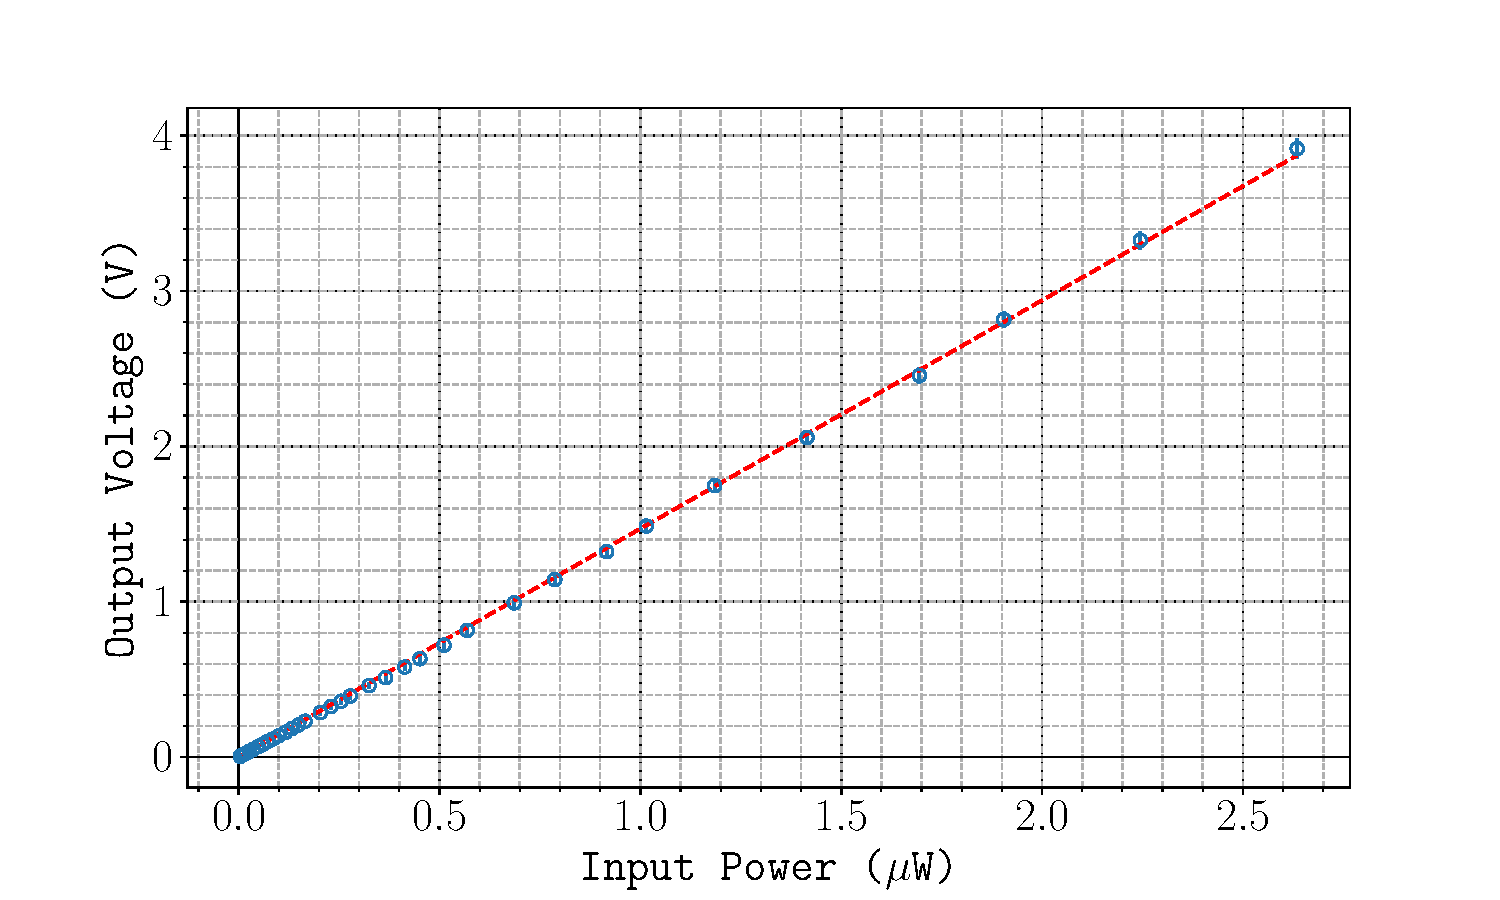
\includegraphics[width=0.8\linewidth]{Figures/Chapter6/pd_calib.pdf}
%  \caption{Name}
%  \label{fig:name}
%\end{figure}
\subsection{Detection using \(\sigma^+\) transitions}\label{subsec:photodiode_setup}
The atoms are detected using resonance fluorescence from the two
vertically aligned \ac{mot} beams in the presence of a vertical
magnetic field. For the \ac{mot} and molasses these are polarised
$\sigma^+$ and $\sigma^-$, but for this detection step, we use a
liquid-crystal \ac{hwp} to give both beams $\sigma^+$ polarisation.
This causes the atoms to be optically pumped into \(\ket{2,2}\) and cycle on the
\(\ket{2,2} \rightarrow \ket{3,3}\) transition, which allows the atoms
to scatter many photons with minimum probability of unwanted optical
pumping into $\ket{F=1}$.
\par\noindent
\FigureRef{fig:detection_scheme} shows the setup used to invert the
polarisation of one \ac{mot} beam prior to detection. The liquid-crystal
waveplate is an electro-optical device whose birefringence changes
when an ac voltage is applied across it. The waveplate is placed at
the output of the downward-propagating (\(\vec{z}_-\))
collimator. The liquid-crystal waveplate is triggered to rotate the
incoming linearly polarised light by $\pi/2$ \sivalue{}{\radian}. 
\begin{figure}[!htpb]
    \centering
    \fontsize{14pt}{14pt}
    \resizebox{0.5\textwidth}{!}{\input{detection_scheme.pdf_tex}}
    \caption[Scheme to invert beam polarisation.]{Scheme to invert
      beam polarisation. In the \ac{mot} loading phase of the
      experiment, the liquid crystal \ac{hwp} is oriented to give a
      right-hand circular polarised beam shown in blue. Prior to
      detection, a digital pulse triggers a re-orientation of its slow
      axis. This results in a left-hand circular polarised beam, shown
      in red.}\label{fig:detection_scheme}
\end{figure}
\subsubsection{Detection Sequence}\label{subsec:detection_sequence}
The sequence used to detect the atoms is shown
in~\FigureRef{fig:detection}. Shortly before the sequence starts, the
bias field is aligned to the \(\vec{z}\) axis and the liquid-crystal
waveplate is triggered to change the handedness of the \(\vec{z}_-\)
beam. The cooling laser frequency is set so it is detuned by
\(\delta_D =\) \sivalue{3}{\mega\hertz}
below the \trans{2}{3} transition and the repump laser is set to
resonance with the \trans{1}{2} transition. This creates an optical
molasses which avoids heating the atoms so that they remain in the
detection volume for a longer period of time. The intensity of the
light is reduced to around \(3 I_\text{sat}\). As shown below, this
intensity was empirically found to minimise the variance in output
voltage. The acquisition of the photodiode voltage is
triggered to start at the first Dwell time. Durin The cooling light is first
switched on without any repump light so that only atoms in \(\ket{F=2}\) scatter light. After this, the repump
is switched on, so that atoms in \(\ket{F=1}\) are optically pumped
into \(\ket{F=2}\) and all the atoms scatter light. Now the
fluorescence measures the total number of atoms $N$. This repump light is a
sideband of the cooling laser, so the total output is increased
to ensure that the intensity of the cooling light remains constant.
Each detection step lasts \sivalue{250}{\micro\second}, but the
first \sivalue{50}{\micro\second} is discarded to allow time for the
intensity to stabilise and for optical pumping into \(\ket{F=2}\).
All the atoms are then blown away by switching off one of the detection
beams before the sequence is repeated to collect a
background signal.
\begin{figure}[!htbp] 
  \centering
  \fontsize{14pt}{14pt}
  \resizebox{0.8\textwidth}{!}{\input{detection.pdf_tex}} 
  \caption[State detection sequence timing]{Timing diagram for state
    detection. Atoms in \(\ket{F=2}\) are detected first, then repump
    light pumps the \(\ket{F=1}\) atoms into $\ket{F=2}$ so they are detected as well. A
background light measurement follows the measurement of the atom
numbers.}
	\label{fig:detection} 
\end{figure}
\subsubsection{Maximum Detection Time}\label{subsubsec:intensity_dependendce}
As the atoms scatter light during detection, the cloud will be heated
and expand due to the momentum exchanged from absorption and
spontaneous emission. The atoms are only cooled along the axis of the
detection beams, so the heating rate is greatest along the other two
axes. It is necessary to ensure that the
heating rate is low enough that the atoms remain within the
detection beam for the entire detection time. A requirement on the
maximum detection time can be obtained as follows. The momentum of
an atom scattering photons follows a random walk, so 
if the cloud has a
Gaussian spatial distribution with an
initial width of \(\sigma_0\), the width at a later time of
is given by
\begin{equation}
\sigma_x^2(t) = \sigma_0^2 + \frac{2 n_p v_r^2 t^2}{3} 
  \label{eq:width_scattering}
\end{equation}
where \(v_r = \frac{\hbar k}{m_\text{rb}} =
\) \sivalue{6}{\milli\metre\per\second} is the recoil velocity and \(n_p\) is the
number of photons scattered. The factor of $2/3$ is because only the
transverse component of the recoil is relevant here. To remain within the detection region,
the width of the cloud must be smaller than the detection beam waist
\(w\), so the detection time must satisfy
\begin{equation}
  t_D \ll \sqrt{\frac{3 \left(w^2-\sigma_0^2\right)}{2 \left(n
  v_r^2\right)}}
  \label{eq:detection_time}
\end{equation}
For a beam waist of \sivalue{7.5}{\milli\metre}, initial cloud size of
\sivalue{5}{\milli\metre} and a maximum scattering rate of
\sivalue{2e7}{\per\second} the detection time must be much less than
\sivalue{4.7}{\milli\second}. This inequality is amply satisfied by
our detection time of \sivalue{100}{\micro\s}.
%\begin{equation}
%  p(x,t) = \int \frac{1}{\sqrt{2\pi} e^{-\frac{(x + \frac{p}{m}
%    t)^2}}{2 \sigma_x^2} \frac{1}{\sqrt{2\pi D t} e^{-\frac{p^2}{2 D
%      t}} \mathrm{d}t
%  \label{eq:prob_atom_diff}
%\end{equation}
\subsubsection{Detection Intensity}
The intensity for detection was chosen by varying the total power
in the detection beams and recording the photodiode voltage for a
fixed detection time of \sivalue{200}{\micro\second}.
\FigureRef{fig:photodiode_intensity_calib} shows the average voltage
measured when detecting atoms in the \(\ket{F=2}\) state as the
intensity of the light increases. The saturation parameter \(s\) is
inferred from the control voltage used control the light
through the \ac{aom} at the output of the
\Muquans laser (see~\FigureRef{fig:muquans_cooling}) and the peak
intensity of the \ac{mot} beams. By the time the atoms are detected,
they have moved away from the region of peak intensity, so the
intensity on the atoms is smaller than the applied control voltage
would indicate if they were at the peak intensity. A fit parameter $b$
is introduced to account for this. A non-linear least squares fit
to the function
\begin{equation}
  v = a\frac{b s}{1 + b s + 4 \left(\delta_D/\Gamma\right)^2}
  \label{eq:voltage_fit}
\end{equation}
gives a scaling for the intensity of \(b = 0.83\). The variance in the
measured voltage (for a constant mean number of atoms) is minimised when the
intensity is around 3\(I_\text{sat}\). Above this intensity, there is
a significant depopulation into \(\ket{F=1}\) caused by off-resonant
excitations to the \(\ket{F'=2}\) state.
This is evident in the voltage signal over time, which is
shown in \FigureRef{fig:detection_time} for various intensities. At an
intensity of 3\(I_\text{sat}\), around 5\% of the population is
pumped out of \(\ket{F=2}\).
\begin{figure}[htpb!]
  \centering
  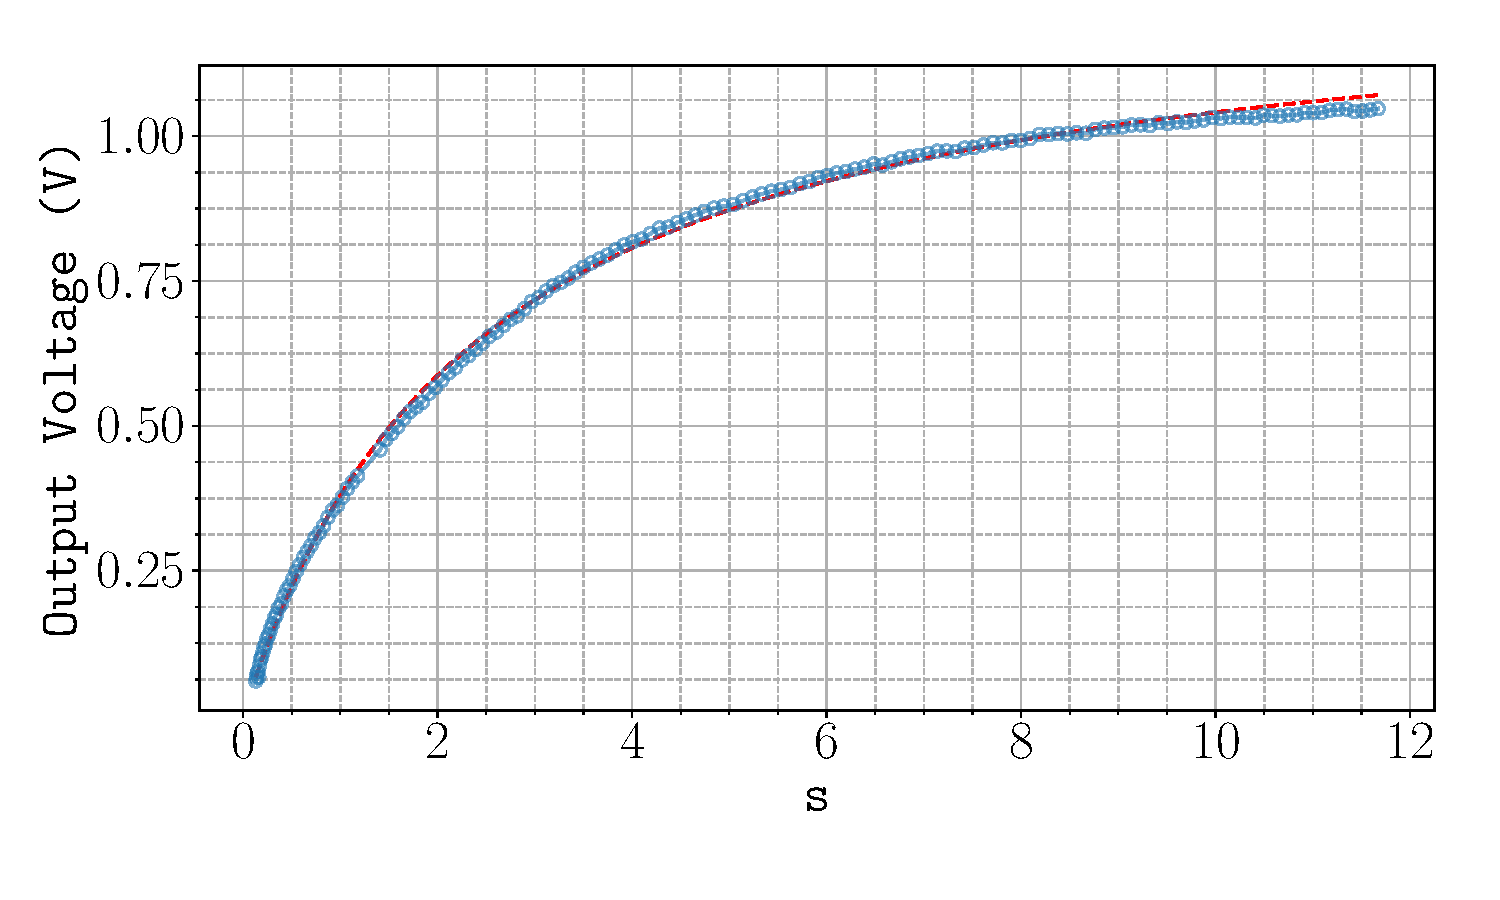
\includegraphics[width=0.7\textwidth]{photodiode_intensity}
  \caption[Photodiode output voltage for increasing detection beam
  intensity. ]{Photodiode output voltage for increasing detection beam
  intensity. The red dashed line indicates a fit
to~\EquationRef{eq:voltage_fit} to estimate the scaling factor for the
saturation parameter \(s\).}
  \label{fig:photodiode_intensity_calib}
\end{figure}

\begin{figure}[htpb!]
  \centering
  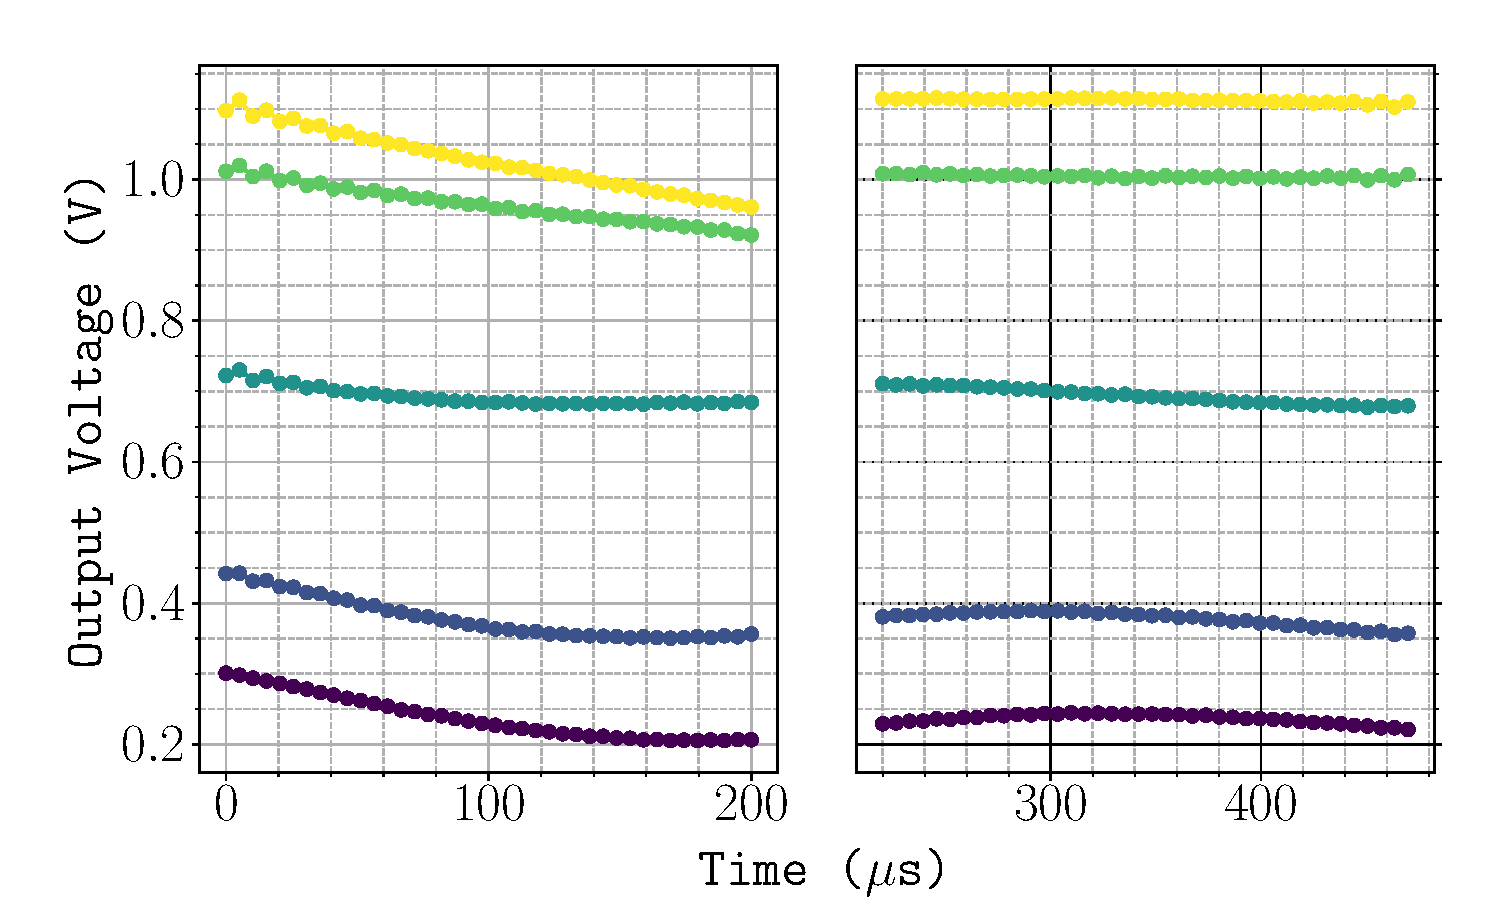
\includegraphics[width=0.7\textwidth]{photodiode_voltage_time}
  \caption[Photodiode voltage for varying detection times.]{Photodiode voltage over time during detection for \(s =
    0.5, 1, 3, 7, 10\) in order from purple to yellow.}
  \label{fig:detection_time}
\end{figure}

\subsection{Measuring the Occupation Probability}\label{subsec:phase_measurement}

The occupation probability of the $\ket{F=2}$ state is obtained by measuring the proportion of
atoms in each hyperfine ground state. The voltage of the amplified
photodiode signal is related to the number of atoms
\(n_\text{at}\) that scatter light on the cycling transition by
\begin{equation}
 V &= \eta R_\text{sc}(s,\delta) n_\text{at} \hbar \omega G 
  \label{eq:pd_signal}
\end{equation}
where \(\eta = \Omega/4\pi\) is the fractional solid angle subtended by the
collection optics, \(\hbar\omega = \sivalue{1.6}{\electronvolt}\) is
the photon energy, \(R_\text{sc}\) is the scattering rate per atom defined
in~\EquationRef{eq:scattering_rate} and \(G\) is the photodiode
conversion gain of \sivalue{1.84e6}{\V\per\W}. At the saturation intensity and a detuning of
\sivalue{3}{\mega\hertz}, the voltage measured per
atom is around \sivalue{30}{\nano\volt} per atom. With a detection
time of \sivalue{200}{\micro\s}, around 7 photons per atom are
detected. The probability of
an atom occupying \(\ket{F=2}\) is estimated as follows
\begin{equation}
  \text{P}_{\ket{F=2}} =
  \frac{\text{N}_2}{\text{N}_\text{Tot}}
  \label{eq:prob_measurement}
\end{equation}
Here the subscript 2 indicates the average voltage measured with
cooling light only (detecting $\ket{F=2}$ atoms) while the subscript
Tot indicates the average voltage with the repump light as well
(detecting all the atoms). 
The interferometer phase difference \(\Delta\Phi\) is determined from \EquationRef{eq:prob_measurement} using
\begin{equation}
  \text{P}_{\ket{F=2}} = \text{P}_0 - \frac{C}{2}\cos(\Delta\Phi)
  \label{eq:interferometer_phase}
\end{equation}
where P\(_0\) is the mean probability of detecting atoms in
\(\ket{F=2}\) and \(C\) is the interferometer fringe contrast. These
are experimentally determined by varying $\Delta\Phi$ as described
in~\SectionRef{sec:fringe_cal}.

\subsubsection{Atom Number Bias}\label{subsec:atom_number_bias}
After the initial state preparation is complete, there are still some
residual atoms left in the states $\ket{F=1, m_F = \pm 1}$. Also, as
shown in~\FigureRef{fig:detection_time}, the photodiode signal that
yields $N_2$ is not constant because some of the $\ket{F=2}$ atoms are
optically pumped into the $\ket{F=1}$ state. In the following, we
consider how both these defects affect the validity
of~\EquationRef{eq:interferometer_phase}.
\par\noindent
If atoms are pumped out of
\(\ket{F=2}\) at a rate \(\gamma\), then the number of atoms in the
number of atoms in $\ket{F=2}$ is given by
\begin{equation}
  n_2(t) = n_{20}e^{-\gamma t}
  \label{eq:n2_time}
\end{equation}
where \(n_{20}\) is the initial number in \(\ket{F=2}\). After
averaging over a time \(\tau\), this gives
\begin{equation}
  N_2 = \frac{n_{20} (1-e^{-\gamma \tau})}{\gamma \tau}
  \label{eq:n2_avg}
\end{equation}
The total number of atoms, measured during the second detection pulse
is
\begin{equation}
  N_\textnormal{Tot} =  n_{10} + n_{20} + n_{\pm 1}
  \label{eq:n1_avg}
\end{equation}
where \(n_{\pm 1}\) is the background population in
\(\ket{1,\pm{1}}\) and $n_{10}$ is the initial population in
$\ket{1,0}$. The detected probability is then
\begin{align}
  \text{P} &= \frac{N_2}{N_\text{Tot}} \nonumber \\
    &= \frac{\frac{n_{20} (1-e^{-\gamma \tau})}{\gamma \tau}}{n_{10} +
    n_{20} + n_{\pm 1}}
    \label{eq:prob_bias}
\end{align}
which is not the same as occupation probability from the
interferometer fringe
\begin{equation}
  \text{P}_0 = \frac{n_{20}}{n_{10} + n_{20}}
\end{equation}
Dividing~\EquationRef{eq:prob_bias} by $n_{10}+n_{20}$, the detected
probability is expressed in terms of $\text{P}_0$ as
follows 
\begin{equation}
  \text{P} = \frac{\text{P}_0}{1+\epsilon}\frac{1-e^{-\gamma \tau}}{\gamma \tau}
\end{equation}
where \(\epsilon = \frac{n_{\pm{1}}}{n_1+n_2}\) is the ratio of the
number of residual atoms to the number in the interferometer.
Similarly, the contrast $C$ of the detected fringe is related to the
actual contrast $C_0$ by 
\begin{equation}
  C = \frac{C_0}{1+\epsilon}\frac{1-e^{-\gamma \tau}}{\gamma \tau}
  \label{eq:contrast}
\end{equation}
For small $\gamma \tau$, this multiplicative factor is
well-approximated by $\frac{1-\gamma \tau}{1+\epsilon}$. 
From~\FigureRef{fig:detection_time}, around 7\% of the signal is lost
for \(s = 3\), so $\gamma = $ \sivalue{360}{\per\s} and $\tau =$
\sivalue{200}{\micro\s}. From the imperfect state preparation, after
velocity selection there is roughly equal population in the $m_F = 0$
state as the $m_F = \pm 1$ states, so we assume $\epsilon = 1$. 
Now the detected contrast is $C = 0.46 C_0$, which includes a factor
of $1/2$ from the $m_F = \pm 1$ atoms. This background population
greatly reduces the detected fringe contrast. Increasing the purity of
the state prior to interferometry will certainly be required to
improve this fringe contrast. 
\section{Individual Pulse Characterisation} \label{sec:atomint_rabiosc}
This section presents a characterisation of the pulses used to drive
Raman transitions between the two hyperfine ground states. First, the
properties of the Raman transition spectrum are presented
in~\SectionRef{subsec:raman_spec}. Following this, a discussion of
cancelling the systematic phase from a differential ac Stark Shift is
given in~\SectionRef{subsec:light_shift}. Finally, this section
concludes with specific details about the individual pulses used in
the experiment. The first Raman pulse, which is used to select a
subset of atoms with a narrow velocity spread, is presented
in~\SectionRef{subsec:vel_select}. This section concludes with a presentation
of the dynamics of the three pulses used to coherently control the
atoms during the interferometer in~\SectionRef{subsec:int_pulses}
\subsection{Raman Transition Spectrum}\label{subsec:raman_spec}
When a circularly polarised light beam excites an atom, the angular
momentum of the light is transferred to the atom. Therefore, a
$\sigma^+$ circularly polarised beam raises the $m_F$ quantum number
by 1 when a photon is absorbed. Similarly, the stimulated emission
induced by a $\sigma^+$ beam lowers $m_F$ by 1. In the case of our
Raman transitions, one beam (with wavevector $\textbf{k}_1$) excites
the atom and another (wavevector $\textbf{k}_2$) stimulates it back
down to the other hyperfine ground state.
\TableRef{tab:raman_polarisation} shows the polarisation selection
rules for these transitions.
\par\noindent
\FigureRef{fig:raman_spectrum} shows an example of the Raman
transition spectrum taken with atoms that have been launched along the
Raman axis at about \sivalue{8}{\cm\per\s}. The beat frequency
between the two Raman lasers is scanned and the light is pulsed for
\sivalue{160}{\micro\second} to drive atoms from $\ket{1,0}$ into the \(\ket{F=2}\)
state. The labels in~\FigureRef{fig:raman_spectrum} indicate the
initial and final $m_F$ values. There is a large narrow peak labelled
$0\rightarrow0$ close to the hyperfine splitting
frequency. This is a result of velocity-insensitive co-propagating
transitions\footnote{When the two light fields are co-propagating, the
  Doppler shift, being proportional to \(\vec{k}_1 -
  \vec{k}_2\) is close to zero}. Looking at the entry
  in~\TableRef{tab:raman_polarisation} for $\Delta m = 0$, this peak
  indicates that the co-propagating beams do not have exactly the
  $\sigma^+ - \sigma^+$ polarisation that was intended. This is further supported by the fact
that there are \(\Delta m = \pm 1\) transitions, which can only occur
if one of the lasers drives a \(\pi\) transition. The Zeeman shifts on
the co-propagating transitions between \(\ket{F=1,0}
\rightarrow \ket{F=2,1}\) and \(\ket{F=1,1}\rightarrow \ket{F=2,1}\)
are \sivalue{95}{\kilo\hertz} and \sivalue{189.5}{\kilo\hertz}, and
are perfectly consistent with the known applied magnetic field of \sivalue{1.4}{\gauss}.
%\begin{table}
%  \centering
%  \begin{tabular}{ccccc}
%    \toprule
%    & & \multicolumn{3}{c}{\(\vec{k}_2\)} \\
%     \midrule
%     & & \(\sigma^-\) & \(\pi\) & \(\sigma^+\)\\
%     \multirow{3}{*}{\(\vec{k}_1\)} & \(\sigma^-\) &  c\(_1\) &
%     c\(_2\)&
%     --  \\
%     & \(\pi\) &c\(_3\) & -- & c\(_4\) \\
%     & \(\sigma^+\) & --& c\(_5\)& c\(_6\)\\
%    \bottomrule
%  \end{tabular}
%  \caption[Raman transition polarisation configurations]{Labels for Raman transitions excited
%    from \(\ket{F=1}\) by \(\vec{k}_1\) and stimulated into
%  \(\ket{F=2}\) by \(\vec{k}_2\).}
%  \label{tab:raman_polarisation}
%\end{table}
\begin{table}
  \centering
  \begin{tabular}{ccccccc}
    \toprule
     & & \multicolumn{5}{c}{\(\ket{F=2,m}\)} \\
     \midrule
     & & -2 & -1 & 0 & 1 & 2 \\
     \multirow{3}{*}{\(\ket{F=1,m}\)} & -1 & (c\(_2\),c\(_4\)) &
     (c\(_1\),c\(_6\)) &(c\(_3\),c\(_6\))& -- & --  \\
     & 0 &-- & (c\(_2\),c\(_4\))& (c\(_1\),c\(_6\)) & (c\(_3\),c\(_6\))
     &-- \\
     & 1 & --& --&(c\(_2\),c\(_4\))& (c\(_1\),c\(_6\)) & (c\(_3\),c\(_6\)) \\
    \bottomrule
  \end{tabular}
  \caption{Allowed polarisation configurations between each hyperfine
  ground state Zeeman sub-levels.}
  \label{tab:raman_polarisation}
\end{table}
\begin{figure}[htpb]
  \centering
  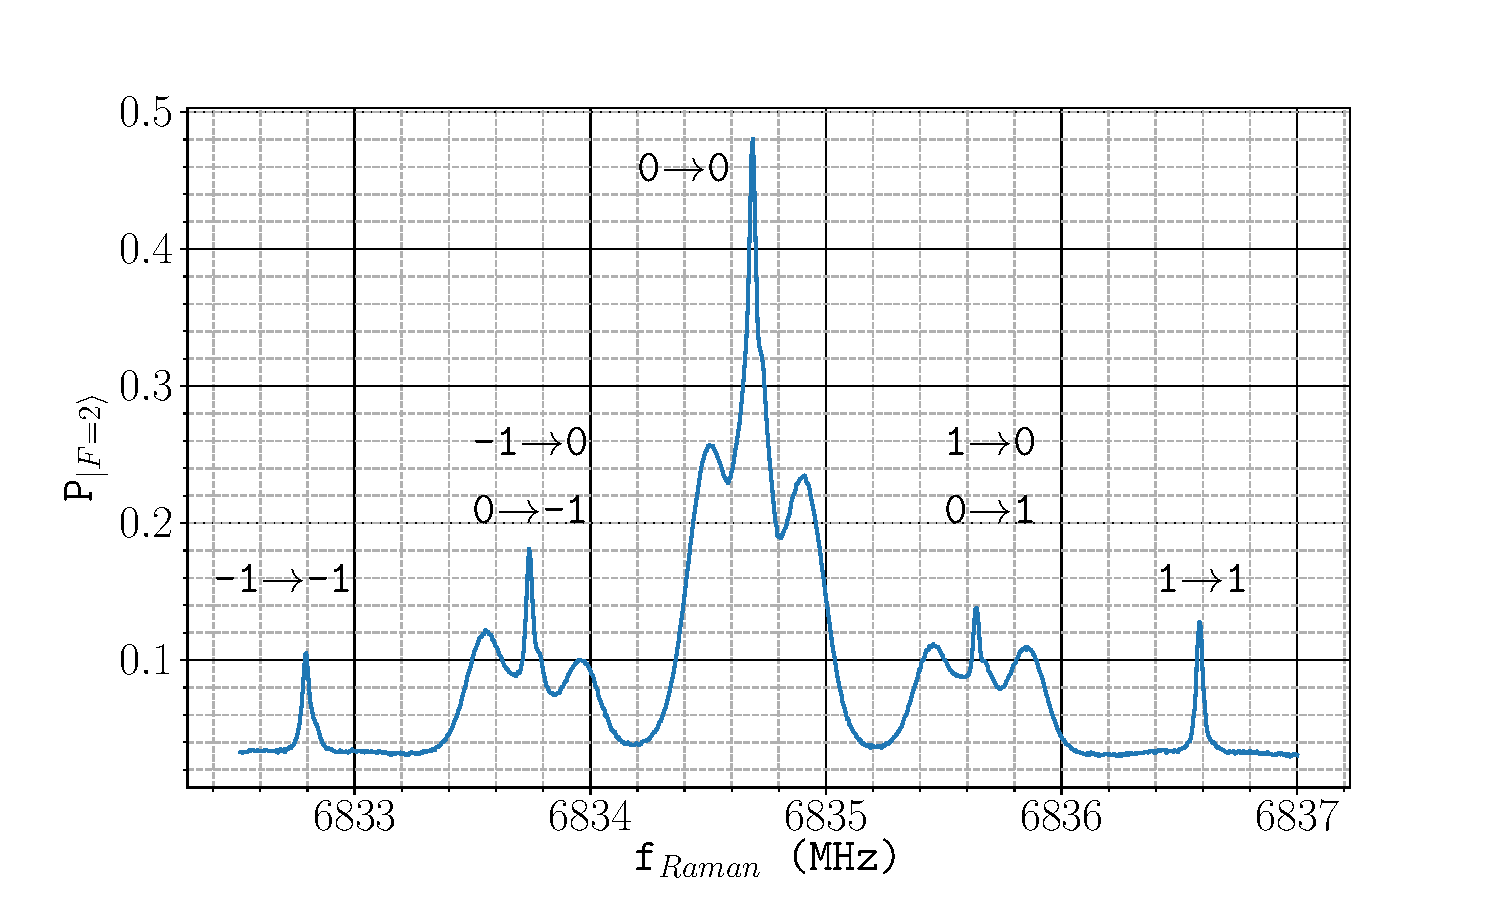
\includegraphics[width=0.7\textwidth]{raman_spectrum}
  \caption[Raman transition spectrum]{Raman transition spectrum, obtained by scanning the beat
    frequency of the two Raman lasers. The transitions \(\ket{1,m_F}
  \rightarrow \ket{2,m_F'}\) are indicated at each observed peak.}
  \label{fig:raman_spectrum}
\end{figure}
\par\noindent
Each narrow transition from \(\ket{1,0}\) has broader
peaks on either side which are the Doppler-sensitive transitions
produced by counter-propagating beams.
The central peak is shown in more detail
in~\FigureRef{fig:raman_spectrum_inset}. The counter-propagating
transitions are shifted from the central co-propagating peak by \sivalue{-185}{\kilo\hertz} and
\(+\)\sivalue{215}{\kilo\hertz} respectively. This difference is
explained by the recoil shift $\Delta f_r = \frac{1}{2\pi}\frac{\hbar
k^2_\textnormal{eff}}{2m} = $ \sivalue{14.9}{\kHz}, which increases
the resonance frequency of both counter-propagating transitions.
After subtracting the recoil shift, the Doppler shifts of
$\pm$\sivalue{200}{\kHz} corresponding to
velocity of \sivalue{7.69}{\centi\metre\per\second}. The same Doppler shifts are also
observed in the peaks corresponding to the \(\ket{F=1,m_F = 0}
\rightarrow \ket{F=2,m_F=\pm 1}\) transitions. The counter-propagating transitions are
Doppler-broadened by the thermal velocity of the atoms along the direction
of the Raman beams. 
%The Doppler shift $\Delta f = \frac{2
%v}{\lambda}$, where $\lambda = $ \sivalue{780}{\nm} broadens the
%transition so that the FWHM is given by
%\begin{equation}
%  \Delta f_\text{FWHM} = 4 \sqrt{2 \ln{2}} \sqrt{\frac{k_B T}{m
%  \lambda^2}}
%\end{equation}
Fitting the transition to the lineshape expected
from a thermal distribution of atoms gives a temperature of
\sivalue{15}{\micro\kelvin} and \sivalue{13.5}{\micro\kelvin} from
each counter-propagating transition. At the time this spectrum was
measured, the molasses was not optimised to give the lowest
temperature.
\begin{figure}[htpb!]
  \centering
  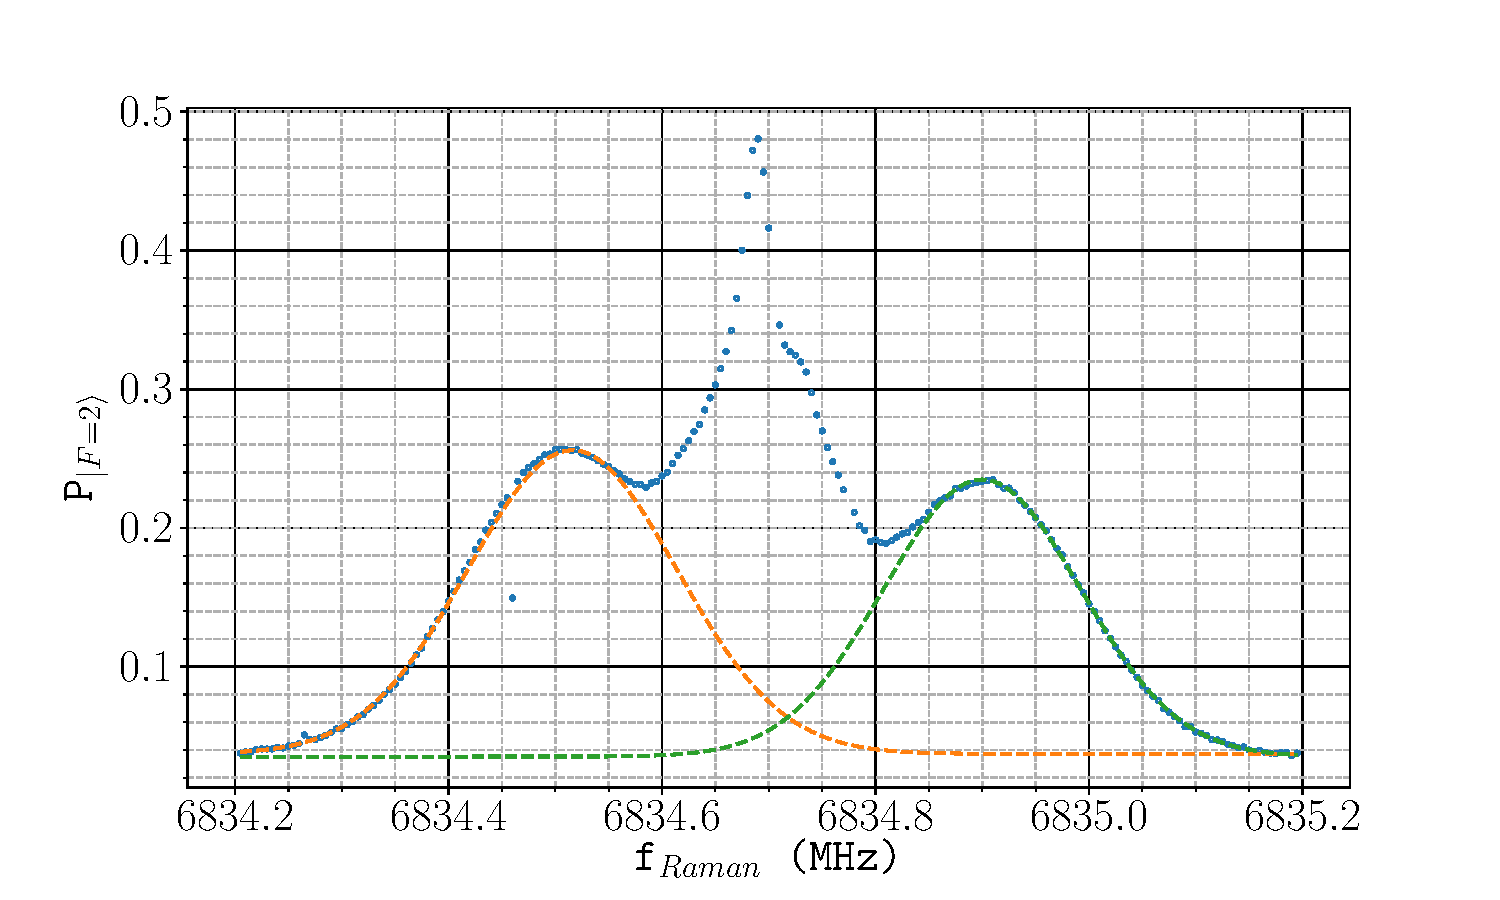
\includegraphics[width=0.7\textwidth]{raman_spectrum_inset}
  \caption[\(\Delta m = 0\) transition spectrum.]{Transition spectrum showing the \(\Delta m = 0\) transition
  from \(\ket{1,0}\). The orange and green dashed lines are fits to a
Doppler-broadened lineshape for each of the counter-propagating
profiles.}
  \label{fig:raman_spectrum_inset}
\end{figure}

\subsection{Cancelling the Differential ac Stark
Shift}\label{subsec:light_shift}
It is worth considering the effects of ac Stark shifts on the atom
interferometer~\cite{Gauguet2008}. They are intrinsically related to the
effective Rabi frequency and as such, cannot be avoided. Each light
beam couples each hyperfine ground state to intermediate states in the
5$P_{1/2}$ and 5$P_{3/2}$ levels in Rubidium-87. The total ac Stark
shift of each level\footnote{The ac Stark shift term
in~\EquationRef{eq:raman_ac_stark} was defined assuming that each
field $\textbf{E}_j$ couples to only one ground state $\ket{j}$. Here,
we do not make that assumption.} is a sum over the shift from each
coupled excited state
\begin{equation}
  \Omega_j^\text{ac} = \sum_{ik} -\frac{|\Omega_{ijk}|^2}{4\Delta_{ijk}}
\end{equation}
in terms of the one-photon Rabi frequencies \(\Omega_{ijk}\) and detunings \(\Delta_{ijk}\) where the index $i = 1,2$ labels each light field, $j = 1,2$ labels
each hyperfine ground state and $k$ labels each excited state that is
coupled by a dipole transition to $j$. From the free evolution of the atom's internal state, there is a contribution to the phase along each path that is
proportional to the sum of the light shifts of each hyperfine ground
state $(\Omega_1^\text{ac} +
\Omega_2^\text{ac})$. For an interferometer pulse separation of $T=
$\sivalue{25}{\ms}, the maximal separation of each path is
$\frac{\hbar k_\text{eff}}{m} T$ = \sivalue{300}{\micro\m}. Close to
the centre of the Raman beams, there is a negligible variation of
intensity over this distance, so the sum of the ac Stark shifts of
each state should not lead to an observable interferometer phase
shift.
\par\noindent
The Raman resonance depends on the difference in energy of the two
states $\hbar(\omega_2 - \omega_1)$. The ac Stark shifts of each state
therefore leads to a contribution to the detuning that depends on the differential ac Stark shift \(\delta^\text{ac}
= \Omega_2^\text{ac} - \Omega_1^\text{ac}\). can lead to an observable
phase shift. Using the results from Ref.~\cite{Weiss1994} for \(\pi\)
and \(\frac{\pi}{2}\) pulses, the phase shift to a Mach-Zender type
interferometer is
\begin{equation}
  \Delta \Phi^\text{ac} =
  \frac{\delta_3^\text{ac}}{\Omega_\text{eff}} - \frac{\delta_1^\text{ac}}{\Omega_\text{eff}} 
 \label{eq:diff_phase}
\end{equation}
where \(\delta_3^\text{ac}\) and \(\delta_1^\text{ac}\) are the ac
Stark shifts of the last and first \(\frac{\pi}{2}\) pulses,
respectively, and $\Omega_\textnormal{eff}$ is the effective Rabi
frequency defined in~\EquationRef{eq:rabi_raman_sum}. Note that there
is no sum over the beam index $k$, because in making the rotating wave
approximation, terms which contain $\Delta_{21k}$ and $\Delta_{12k}$
are dropped as they oscillate much faster than the retained terms. 
\par\noindent
As the atoms fall
under gravity, they move through the Raman beam profile and experience
the interferometer pulses at different intensities. To the extent that
there is a light shift of the clock transition, this can produce a
non-zero interferometer phase. Fortunately, it is possible
to eliminate such a shift using an appropriate choice
of intensity and detuning of the Raman lasers. This can be seen by
first writing out the differential ac Stark shift
\begin{equation}
  \delta^\text{ac} = \Omega_1^\text{ac} - \Omega_2^\text{ac} = \sum_{ik}
  \frac{\lvert\Omega_{i1k}\rvert^2}{4\Delta_{i1k}} - \sum_{ik}
  \frac{\lvert\Omega_{i2k}\rvert^2}{4\Delta_{i2k}} 
  \label{eq:diff_shift}
\end{equation}
When both Raman beams are red-detuned from
all the one-photon transitions, both terms
in~\EquationRef{eq:diff_shift} are strictly negative. Therefore,
\(\delta^\text{ac}\) can be cancelled by choosing the correct
intensities for each Raman beam. A plot of \(\delta^{\text{ac}}\)
for various Raman beam intensities as a function of the ratio between
the two Raman beams is shown in~\FigureRef{fig:light_shift_ratio}. There
is a ratio at which the differential ac Stark shift cancels and is
independent of the total intensity. The one-photon detuning $\Delta_R$
is defined such that the laser frequency $\omega_2^l$ is detuned from
the \trans{2}{3} transition (in the absence of light shifts) by
$\Delta_R$. The ratio that cancels
\(\delta^\text{ac}\) for increasing \(\Delta_R\) is shown
in~\FigureRef{fig:light_shift_detuning}. When \(\Delta_R\) is
\sivalue{1.13}{\giga\hertz} below the \trans{2}{3} transition, this
ratio is maximised. The differential ac Stark shift is cancelled when
the intensity ratio of light driving \(\ket{1,0}\) transitions to
\(\ket{2,0}\) transitions is \(\mathcal{R} = 0.583\). 
\begin{figure}[htbp!]
	\centering
	\def\svgwidth{\columnwidth}
	\subfloat[][]{\scalebox{0.45}{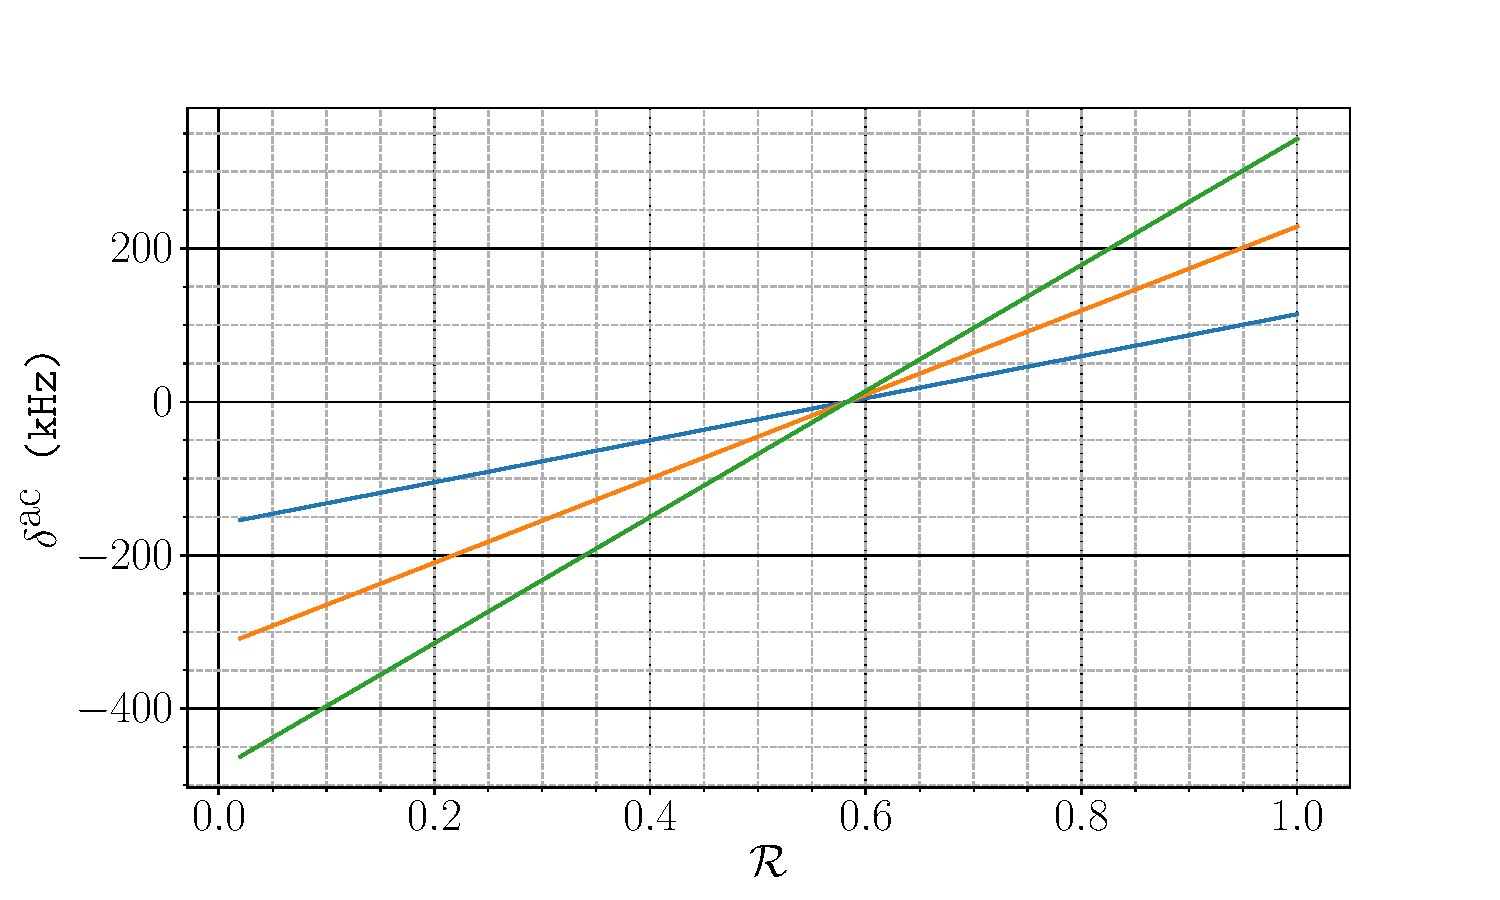
\includegraphics{light_shift_ratio}}\label{fig:light_shift_ratio}}\\
\subfloat[][]{\scalebox{0.45}{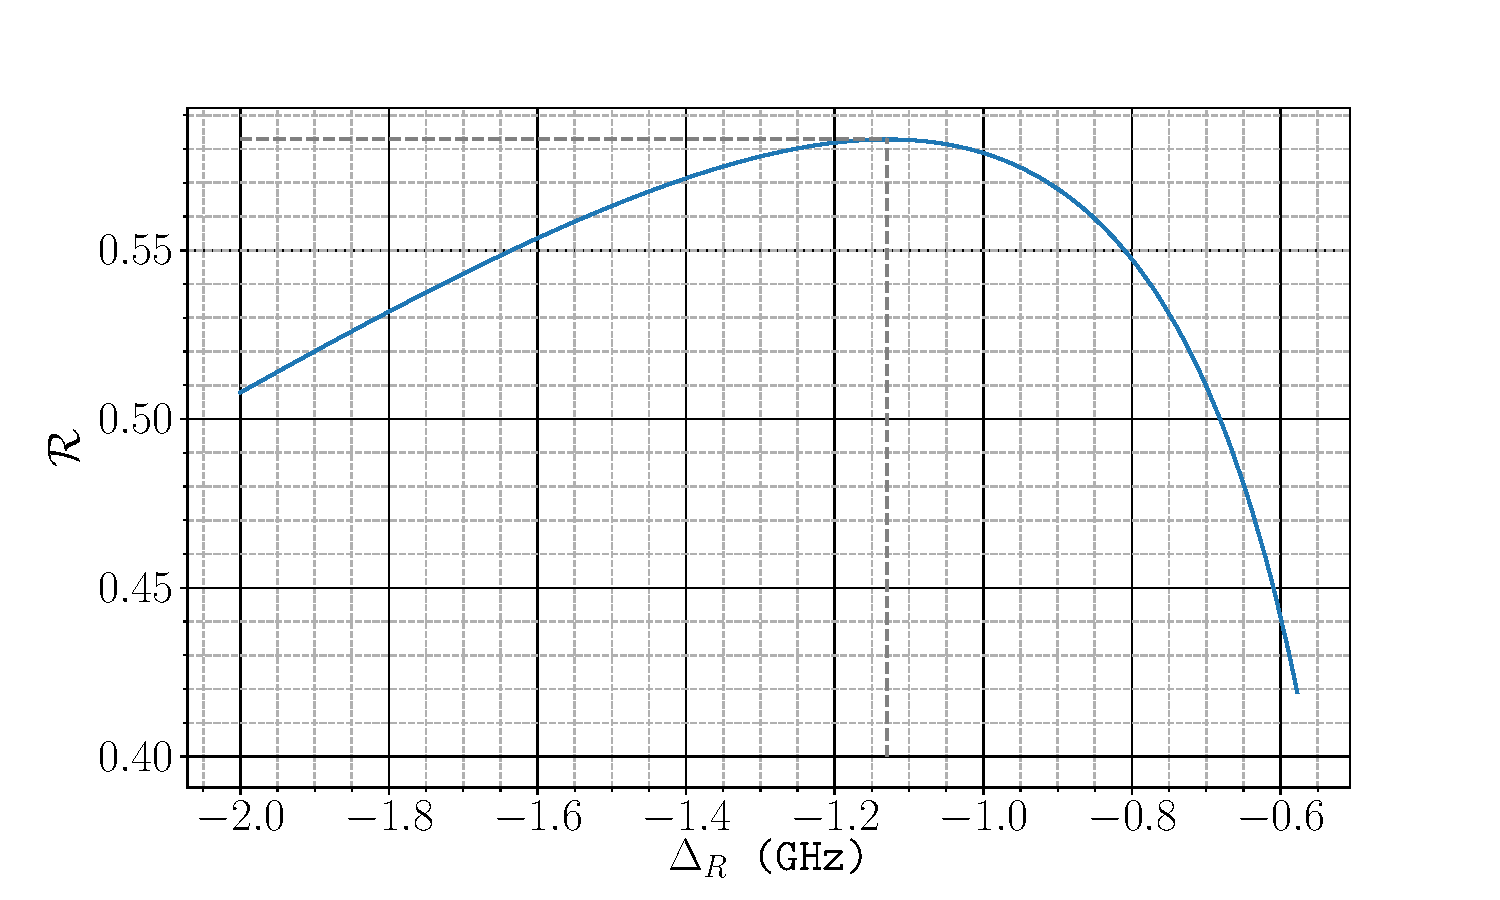
\includegraphics{light_shift_detuning}}\label{fig:light_shift_detuning}}\\
	\caption[Differential ac Stark shift as a function of two-photon
  detuning and Raman beam intensities.]{The effects of the Raman beam
  intensities and detuning on the differential ac Stark shift
  \(\delta^\text{ac}\).
\textbf{(a)} shows \(\delta^\text{ac}\) as a function of the intensity ratio
\(\mathcal{R}\) between the light which drives transitions from
\(\ket{1,0}\) to the light that couples to \(\ket{2,0}\) for the
two-photon detuning of \(\Delta_R = -\sivalue{1.13}{\giga\hertz}\)
used in the experiment. Example
intensities for the \(\ket{2,0}\) light are
\sivalue{100}{\watt\per\metre\squared} (blue),
\sivalue{200}{\watt\per\metre\squared} (orange) and
\sivalue{300}{\watt\per\metre\squared} (green). \textbf{(b)} shows how
the ratio for which \(\delta^\text{ac} = 0\) varies as \(\Delta_R\)
increases. The dashed lines indicate the value of \(\Delta_R\) used in
the experiment and its corresponding ratio of 0.583.}
	\label{fig:light_shift_plots}
\end{figure}
\par\noindent
It is not straight-forward to directly measure the intensity of
each Raman beam on the atoms, so the transition spectrum was used to cancel the
differential ac Stark shift and determine when the intensities of the
lasers are set to the appropriate
ratio. Experimentally, this was done by adjusting the power of the
pump lasers for the master and slave SolsTiS lasers. When the master
is seeded with \sivalue{10}{\watt} and the slave with
\sivalue{6.5}{\watt}, the differential ac Stark shift is eliminated.
\FigureRef{fig:cancelled_light_shift} shows the transition spectrum using two different effective Rabi
frequencies, corresponding to \(\pi\) pulse times of
\sivalue{22.5}{\micro\second} and
\sivalue{45}{\micro\second}. In this instance, the frequency difference of the two
co-propagating peaks, shown in blue and orange, is less than \sivalue{1}{\kilo\hertz}.
\begin{figure}[htpb!]
  \centering
  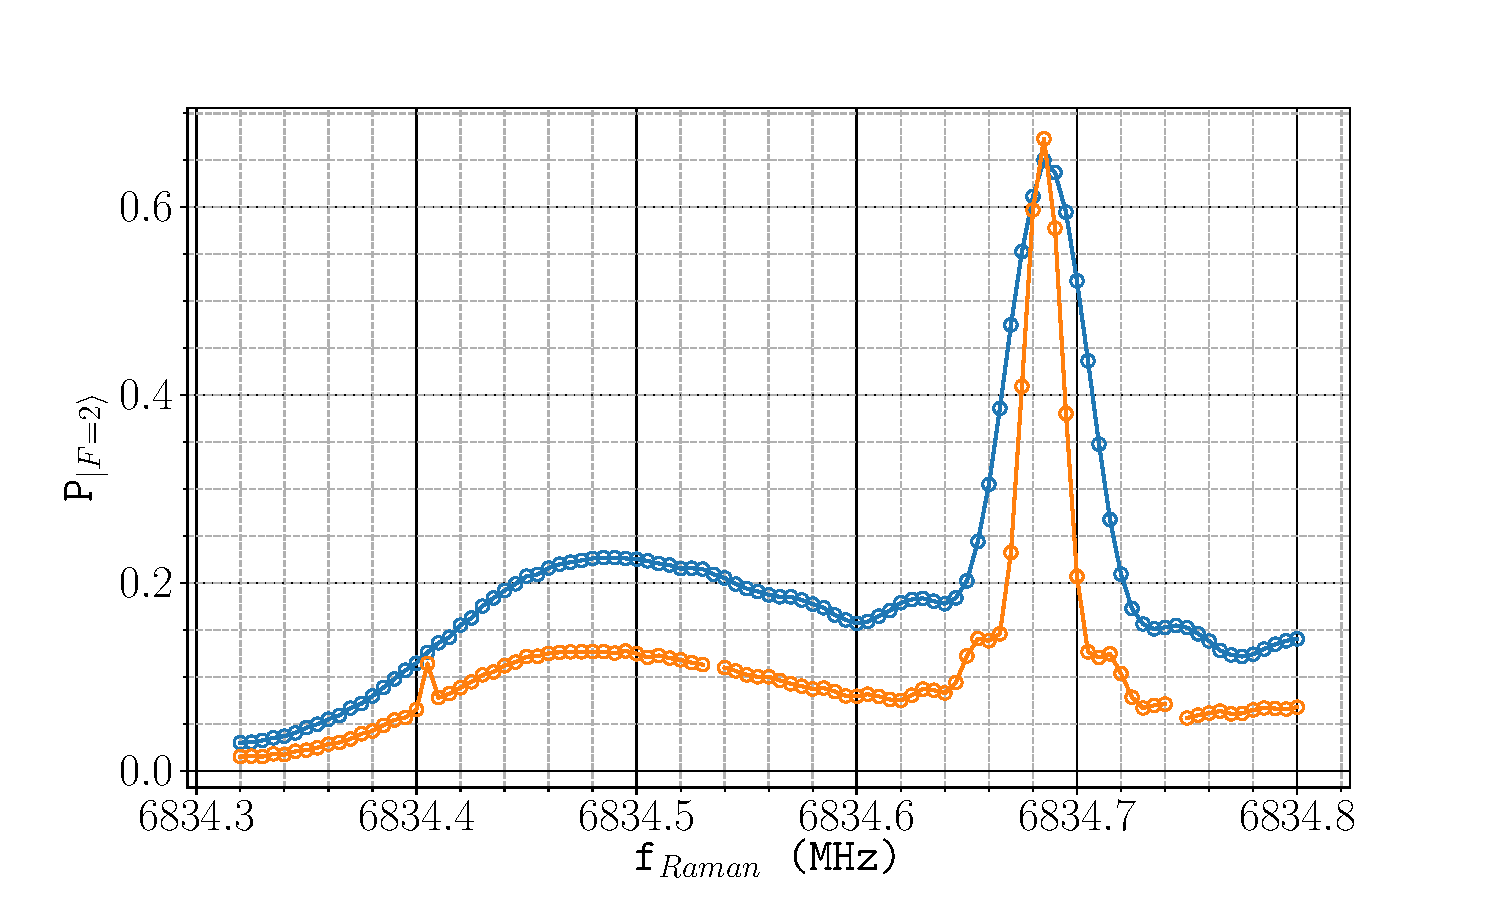
\includegraphics[width=0.7\textwidth]{cancelled_light_shift}
  \caption[Raman transition spectrum after cancelling the differential
  ac Stark shift.]{Raman transition spectrum after cancelling the differential
    ac Stark shift. The blue curve shows a pulse with a \(\pi\) pulse
  time of \sivalue{22.5}{\micro\second} and the orange shows the
  spectrum using a less intense pulse with a $\pi$-pulse time of
\sivalue{45}{\micro\second}.}
  \label{fig:cancelled_light_shift}
\end{figure}
There is also a shift of \sivalue{1.4}{\mega\hertz} from
\(f_\text{hfs}\).
This is a result of a
second-order Zeeman shift and corresponds to a field strength of
\sivalue{1.56}{\gauss}.
\subsection{Velocity-Selective Pulse}\label{subsec:vel_select}
The accelerometer has to use the velocity-sensitive transitions
induced by counter-propagating beams in order to be sensitive to
acceleration. In order for all the atoms to experience the same
desired pulse areas of $\pi/2-\pi-\pi/2$, it is necessary for the
Doppler width to be much less than the natural width arising from the
duration of the Raman pulses. In this apparatus, the laser cooling
gives a temperature of \sivalue{6}{\micro\kelvin}, for which the Doppler
width (FWHM) is \(\sigma_f = \frac{4 \sqrt{2 \ln(2)}}{\lambda}\sqrt{\frac{k_b T}{m}}
\approx\) \sivalue{140}{\kilo\hertz}. 
A $\pi$-pulse duration of \sivalue{6}{\micro\second} gives a
linewidth close
to this Doppler width, but the intensities required for this are above
what is attainable with our Raman laser. 
\par\noindent
We therefore reduce the Doppler width of the participating atoms
by first applying a long Raman pulse to select a subset of the population
with a narrower velocity spread~\cite{Moler1992}. This
velocity-selective pulse gives a narrower Doppler linewidth than the
subsequent shorter
interferometer pulses thereby ensuring that the Rabi frequencies are
reasonably homogeneous across the cloud of selected atoms.
\par\noindent 
Starting with a velocity distribution of atoms
described by a 1-D Maxwell-Boltzmann distribution all occupying the
\(\ket{1,0}\) state, the
population in \(\ket{2,0}\) after applying a Raman pulse is
distributed according to
\begin{equation}
  \text{P}_{\ket{2,0}}(v) = \frac{\Omega_\textnormal{eff}^2}{\Omega_\textnormal{eff}^2 + \delta^2}
  \sin\left(\sqrt{\Omega_\textnormal{eff}^2+\delta^2}\;\tau\right)^2 p(v)
  \label{eq:vel_selected_dist}
\end{equation}
where \(\delta\) is the Raman detuning defined
in~\EquationRef{eq:raman_detuning}, \(p(v) = \sqrt{\frac{m}{2\pi
k_B T}} e^{-\frac{m v^2}{2 k_B T}}\) is the velocity distribution and
\(\Omega_\textnormal{eff}\) is the effective Rabi frequency defined
in~\EquationRef{eq:rabi_raman_sum}. \FigureRef{fig:vel_selected_dist}
shows the expected
distribution of Doppler shifts in the selected atoms after a
\sivalue{6}{\micro\K} cloud has been driven by a $\pi$ pulse with a duration of
\sivalue{40}{\micro\second}.
The population that is stimulated
has a mean velocity shifted by twice the recoil velocity. In this
instance, the rms
Doppler shift is \(\sigma_f
=\)\sivalue{19.7}{\kilo\hertz}.
\begin{figure}[htpb!]
  \centering
  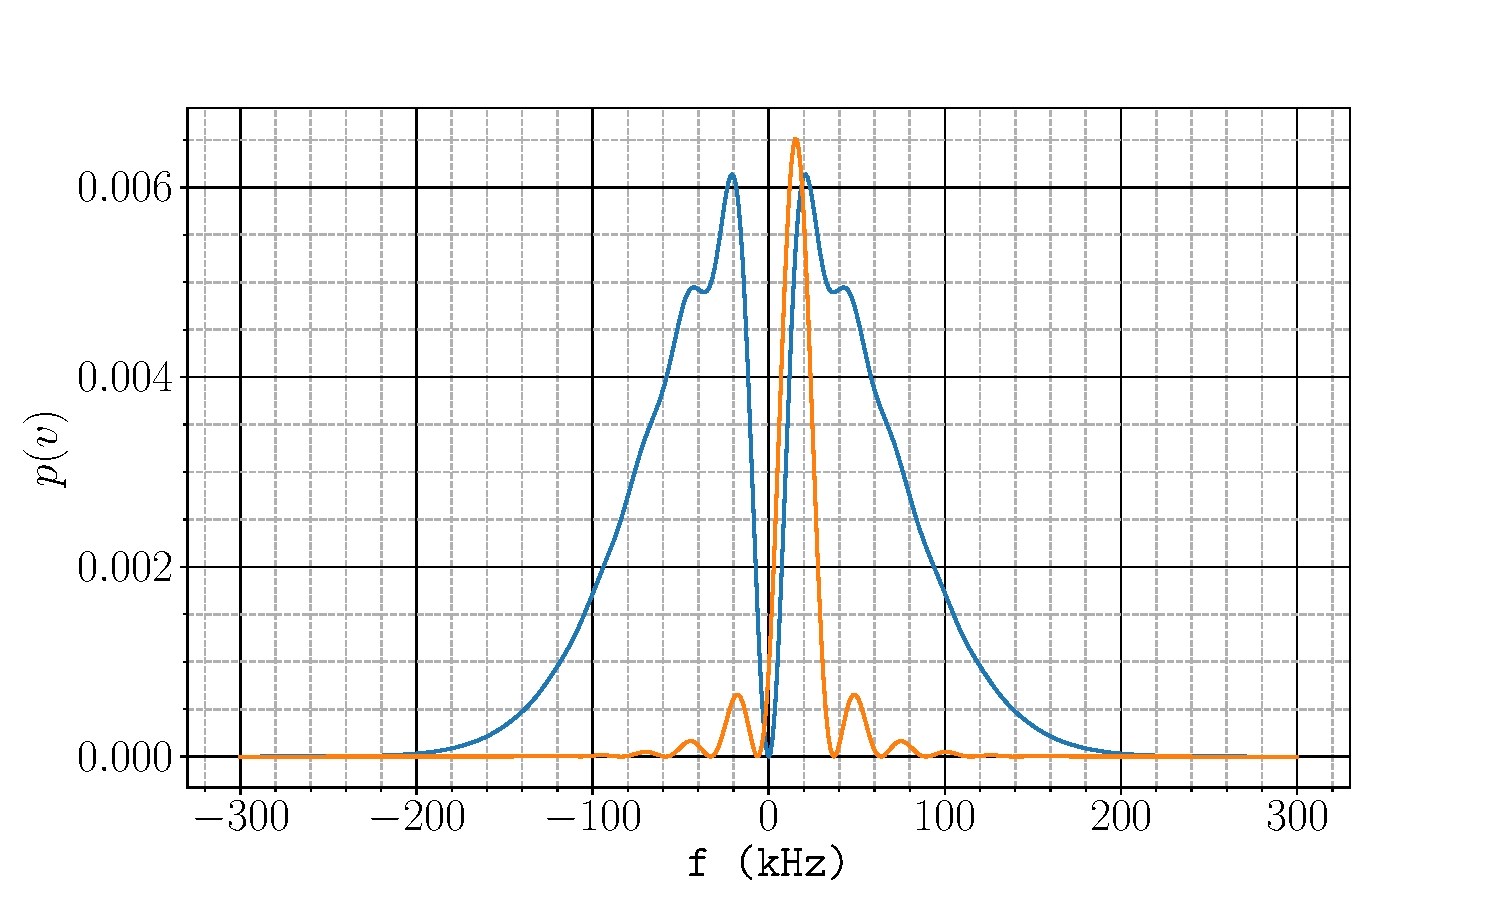
\includegraphics[width=0.7\textwidth]{vel_selected_dist.pdf}
  \caption[Simulated velocity distribution after a Raman $\pi$
  pulse.]{Calculated distribution of frequency shifts in the ensemble
    selected from a \sivalue{6}{\micro\kelvin}
  cloud by a \sivalue{40}{\micro\second} Raman \(\pi\)
pulse. Blue curve: atoms not selected. Orange curve: atoms selected.
Note the recoil shift of the selected atoms in addition to their
Doppler shifts. }
  \label{fig:vel_selected_dist}
\end{figure}
\subsubsection{Velocity-Selected Distribution}
The velocity distribution of atoms after the velocity selective pulse
can be measured using a second Raman pulse as a probe. This probe must
be much longer duration than
the velocity-selection pulse so that it gives even narrower
resonances. 
\FigureRef{fig:vel_select_chirp} shows a measurement of the transition
spectrum close to the peak of the Doppler-sensitive transition that is
greater in frequency than the Doppler-insensitive peak. The orange
curve shows the spectrum obtained before velocity selection, using a single Raman $pi$ pulse of
duration \sivalue{40}{\micro\s}. The blue curve, which illustrates the
distribution of atoms after velocity selection, is obtained by first
applying a
\sivalue{40}{\micro\second} \(\pi\) pulse with a Raman beat frequency
\(f_v = \) \sivalue{6834.51}{\mega\hertz}. This prepares atoms in
\(\ket{1,0}\), then the atoms which remain in
\(\ket{F=2}\) are blown away. After \sivalue{10}{\milli\second}, a
\sivalue{80}{\micro\second} \(\pi\) pulse transfers some of the
remaining population back into \(\ket{2,0}\). The frequency of the
probe pulse is varied by chirping the Raman laser beat frequency. In
this instance, the power of the \sivalue{80}{\micro\s} pulse was not tuned to give a \(\pi\)
pulse area so the measured population is not indicative of the maximum
driven by the Raman transition. The red curve shows a fit to a
Doppler-broadened lineshape, which gives an effective temperature
of around \sivalue{1}{\micro\K}. Comparing this to the peak from
before velocity selection, it is clear that the velocity
distribution of the selected atoms is much narrower. 
\begin{figure}[htpb!]
  \centering
  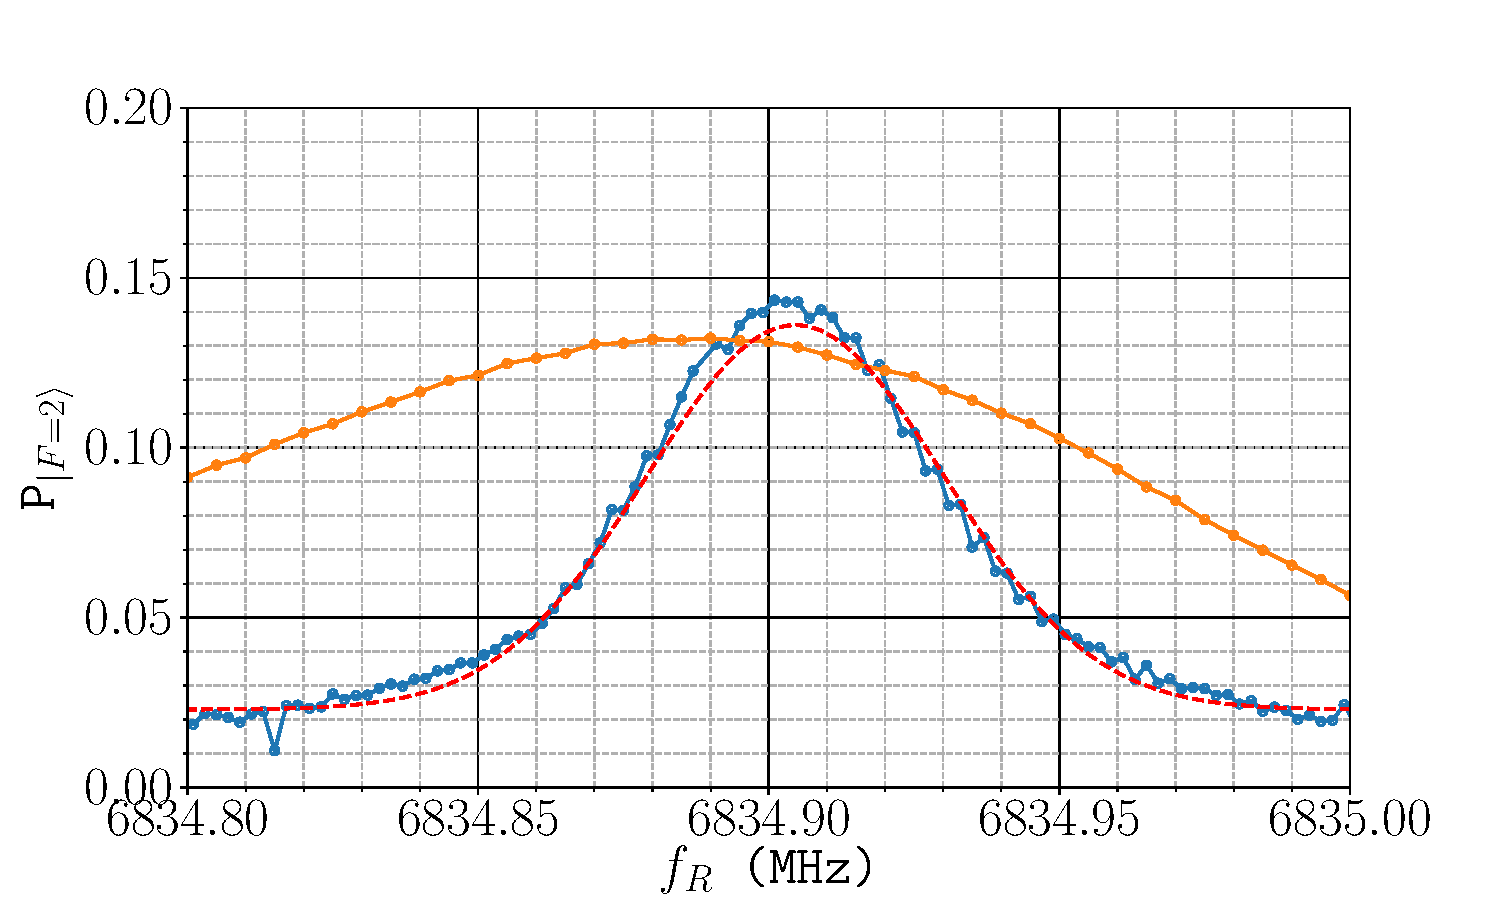
\includegraphics[width=0.7\textwidth]{RamanChirp.pdf}
  \caption[$\ket{F=2}$ population after a velocity-selective Raman
  $\pi$ pulse.]{\(\ket{F=2}\) population after a Raman pulse at a frequency
    \(f_v =\)\sivalue{6834.51}{\mega\hertz} transfers atoms to
    \(\ket{1,0}\). This distribution is probed by
  applying a narrow pulse at a frequency \(f_{R}\). The population
measured in \(\ket{F=2}\) is shown in blue. The red dashed line is a
fit to the Doppler-broadened
transition peak. The orange curve shows
transition spectrum (without velocity selection) from a $pi$-pulse
of duration \(\tau = \)\sivalue{40}{\micro\s}.}
  \label{fig:vel_select_chirp}
\end{figure}
\subsection{Interferometer Pulses}\label{subsec:int_pulses}
The power settings needed to make Raman $\pi$ and $\pi/2$ pulses were
empirically determined by observing Rabi oscillations. These are shown
in~\FigureRef{fig:rabi_oscillation}. For a $\pi$ pulse, the Raman
laser power was
set so that the Rabi oscillation reached its maximum after a pulse duration of
\(\tau = \)\sivalue{15}{\micro\s}. It is clear that the oscillations
are rapidly damped. This dephasing rate depends on the
time at which the pulse is applied. Since the atoms are at different
positions in the beam, this suggests that the dephasing is caused by a
spatial variation of the Rabi frequency. This is largely a result of
irregularities in the Raman beam intensity profile from defects in
the two small aspheric lenses. The Gaussian intensity distribution of each beam
is unlikely to cause such a fast dephasing, since the atoms remain
close to the centre of the beam. At longer pulse durations,
spontaneous decay from the intermediate states of the Raman transition
becomes apparent.
\begin{figure}[htpb]
  \centering
  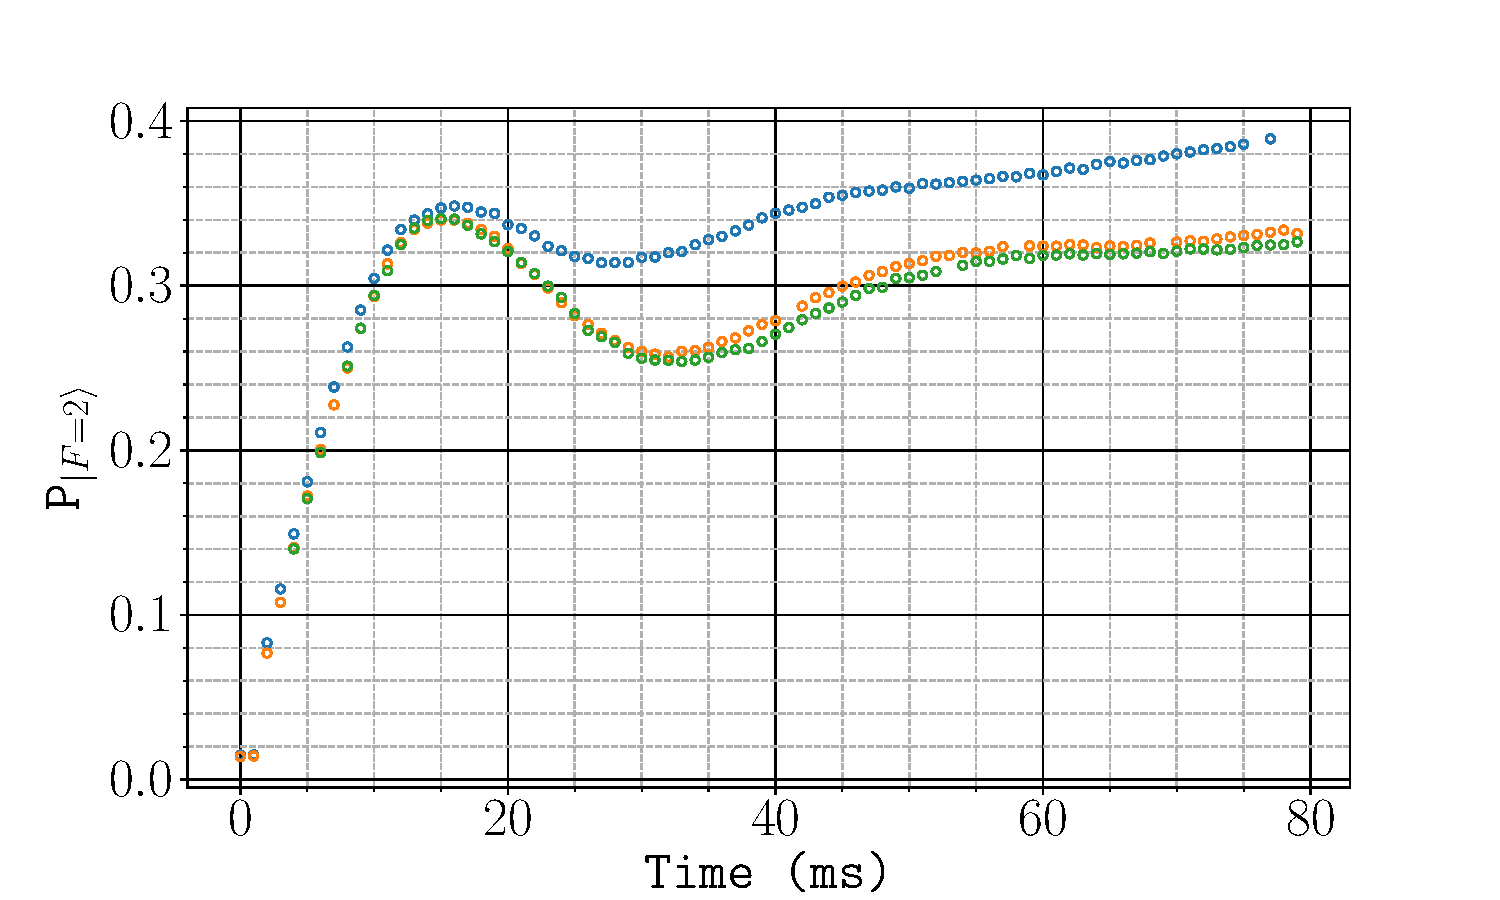
\includegraphics[width=0.8\linewidth]{SinglePulses.pdf}
  \caption[Rabi oscillations between the $\ket{1,0}$ and $\ket{2,0}$
    states.]{Rabi oscillations between the $\ket{1,0}$ and $\ket{2,0}$
    states. Each pulse occurs at different times after the \ac{mot} is
    released. The times shown are \sivalue{13}{\ms} (blue),
  \sivalue{23}{\ms} (orange) and \sivalue{33}{\ms} (green). Full
  population transfer is not observed due to the atoms in $\ket{1,\pm
1}$ which have not been removed. }
\label{fig:rabi_oscillation}
\end{figure}
\section{Noise}\label{sec:atomint_sensitivity}
This section presents a discussion of the identified sources of
noise in the interferometer and their effects on the sensitivity to
accelerations. It begins with a discussion of the noise that arises
from detecting atoms in~\SectionRef{subsec:detection_noise}. This
defines an uncertainty in measuring the occupation probability, which then used to
express the corresponding acceleration uncertainty
in~\SectionRef{subsec:accel_uncert}. The Allan variance used to characterise
the stability of the interferometer signal is defined
in~\SectionRef{subsec:allan_variance}. The sensitivity function and an analytic method
for calculating the influence of random phase fluctuations is given
in~\SectionRef{subsec:sens_func}. This is applied to phase noise from
the Raman laser in \SectionRef{subsec:laser_phase} and external
vibrations in~\SectionRef{subsec:vibration_noise}. Finally, the
section concludes with a summary of the identified sources of noise
in~\SectionRef{subsec:noise_sources}.
\subsection{Detection Noise}\label{subsec:detection_noise}

Each measurement of the number of atoms has an uncertainty due to
random processes that influence the voltage measured by the detector. These errors
combine to give an uncertainty in the interferometer phase and
hence, acceleration. It is worth distinguishing between the different
sources of noise in measuring the occupation probability
$\text{P}_{\ket{F=2}}$. Fluctuations in the number of atoms and detected
photons lead to an uncertainty in the measured voltages that
correspond to $N_2$ and $N_\text{Tot}$. It is essential that the
photo-detector used is sensitive enough to ensure that this does not
limit the sensitivity~\cite{Rocco2014}. A more fundamental limitation
is the noise that arises when an atom is projected into either the
$\ket{1,0}$ state or the $\ket{2,0}$ state. In what follows, these
three sources of detection noise are discussed in the context of the
detection sequence previously described
in~\SectionRef{subsec:detection_sequence}. 
\subsubsection{Atom and Photon Number Fluctuations}
The random processes by which atoms are loaded and cooled in the
initial stages of the experiment, as well as the random direction a
photon is spontaneously emitted mean that both the total number of
atoms after interferometry and the number of photons arriving at the
detector within a given time duration will have shot noise
fluctuations. The voltage measured by the detector, as defined
in~\EquationRef{eq:pd_signal}, is proportional to the number of atoms
scattering the incident light. Therefore, the variance in the measured
voltage due to atom and photon shot noise fluctuations are 
\begin{align}
  \sigma_\text{at,v}^2 &= \alpha^2 \eta^2 R_\text{sc}^2 n_\text{at}\\
  \sigma_\text{p,v}^2 &= \alpha^2 \eta R_\text{sc} n_\text{at} 
  \label{eq:atom_photon_noise}
\end{align}
where $\alpha = \hbar \omega G$ and the subscripts ``at'' and ``p'' refer to atoms and photons,
respectively. Of the two, \(\sigma_\text{at,v}\) dominates provided at least one photon
per atom is detected. As previously discussed
in~\SectionRef{subsec:photodiode_setup}, around 7 photons per atom
are detected, so this is certainly the case. For the detection parameters previously defined, the shot noise is equal to around \sivalue{46.5}{\nano\volt} per atom. 
The standard deviation of the detected voltage during background light
measurements was on the order of \sivalue{80}{\micro\volt}. Since at
least \num{1e6} atoms are detected, the noise from background light
fluctuations is negligible.  

\subsubsection{Quantum Projection Noise}
The occupation probability $\text{P}_{\ket{F=2}}$ is determined by measuring the ratio
$\frac{N_2}{N_\text{Tot}}$. In
measuring both the number of atoms in $\ket{F=2}$ and the total number of atoms, the contribution of atom shot
noise to an uncertainty in $\text{P}_{\ket{F=2}}$ is suppressed. However, for a
fixed number of atoms there is still an uncertainty due to the
projection of an atom's internal state onto the $\ket{1,0}$ and
$\ket{2,0}$ states. This is the standard quantum limit -- the minimum
uncertainty that can be reached for an ensemble of atoms prepared in
the same internal state~\cite{Bollinger1996}. 
To derive the uncertainty in $\text{P}_{\ket{F=2}}$, we first make the assumption
that there are atoms in $m_F=\pm 1$, as
in~\SectionRef{subsec:atom_number_bias}, which are detected but do not
contribute to the interferometer. The total number of atoms is
$N_\text{Tot}$. Similarly, $n_2$ atoms detected in $\ket{F=2}$, which
has an average value denoted as $\langle N_2 \rangle$ and a mean
occupation probability $\langle p_2 \rangle$. If $n_{10}$ is the
number atoms prepared in $\ket{1,0}$, it follows that the mean and
variance of $n_2$ are given by
\begin{align}
  \langle N_2 \rangle &= \langle p_2 \rangle \\
  \Delta N_2 &= n_{10} \Delta p_2 = n_{10} \langle p_2 \rangle \langle
  p_1 \rangle \label{eq:proj_noise}
\end{align}
where $\langle p_1 \rangle$ is the average occupation probability of
$\ket{F=1}$ after interferometry. The measured probability is given by
\begin{align}
  \text{P}_{\ket{F=2}} &= \frac{\langle p_2 \rangle n_{10} \pm \sqrt{n_{10}
  \langle p_2 \rangle \langle p_1 \rangle}}{n_{10}(1+\epsilon)}
  \nonumber \\
                &= \frac{\langle p_2 \rangle}{1+\epsilon} \pm
                \frac{1}{1+\epsilon} \sqrt{\frac{\langle p_2 \rangle
                \langle p_1 \rangle}{n_{10}}} 
                \label{eq:prob_noise}
\end{align}
where as before $\epsilon$ is the ratio of the number of atoms in $m_F = \pm 1$ to
the number in the interferometer and it is assumed that this ratio
does not fluctuate. Without any inhomogeneity in the
Rabi frequency\footnote{Atoms which experience different pulse areas
  have different phase shifts. The interferometer signal is a
convolution of these. In which case, the contribution to the detection
noise from the projection noise of each atom is less straight-forward.
For simplicity, it is assumed here that the only loss
in fringe contrast is due to background atoms.}, the average occupation probabilities are 
$\langle p_2 \rangle = \sin^2(\Delta \Phi/2)$ and $ \langle p_1
\rangle = \cos^2(\Delta \Phi/2)$. In terms of the interferometer phase
difference $\Delta \Phi$, \EquationRef{eq:prob_noise} becomes
\begin{equation}
  \text{P}_{\ket{F=2}} = \frac{1-\cos(\Delta \Phi)}{2(1+\epsilon)} \pm
  \frac{1}{2(1+\epsilon)}\frac{\sin(\Delta \Phi)}{\sqrt{n_{10}}}
\end{equation}
A useful measure of the interferometer's sensitivity is given by the
ratio of the noise to the fringe amplitude which is
\begin{equation}
  S = \frac{\sin(\Delta\Phi)}{\sqrt{n_{10}}}
  \label{eq:sens_proj}
\end{equation}
and is independent of $\epsilon$. At the mid-point
of a fringe $\Delta \Phi = \frac{\pi}{2}$, this is maximised and the
interferometer is most sensitive to changes in $\Delta \Phi$. A
relation between the uncertainty in $\text{P}_{\ket{F=2}}$ and the
interferometer phase is derived in~\SectionRef{subsec:accel_uncert}.

\subsubsection{Photodiode Technical Noise}
In order for the detection noise
be dominated by the quantum projection noise, the detector must be sensitive
enough that it has a \ac{nep} much lower than the noise in the optical
power detected. The \ac{nep} of a detector is defined as the
equivalent optical power which gives a signal-to-noise ratio of 1
after an integration time of \sivalue{0.5}{\second}. The photodiode
signal is amplified so it is convenient
to express the technical noise as a voltage density, by multiplying it by the
amplifier gain. Hence, the
voltage density of a detector whose sensitivity is equivalent to the
voltage corresponding to the quantum projection noise for an
integration time \(\tau_D\) is given by
\begin{equation}
  V^2_\text{at} =
  \frac{1}{2\tau_D}\eta \hbar \omega G R_\text{sc}\Delta N_\text{proj}
  \label{eq:nep}
\end{equation}
where $\Delta N_\text{proj} = \sqrt{N_\text{proj}}$ is the variance in
the number of atoms detected due to the projection of atoms onto the
states $\ket{1,0}$ and $\ket{2,0}$. If the signal is detected for $\tau_D =$ \sivalue{200}{\micro\s},
multiplicative factor that relates $V_\text{at}$ to
$\Delta N_\text{proj}$ is \sivalue{6.7e-12}{\volt\squared\per\hertz}.
\par\noindent
Technical noise in the detector typically arises from multiple electronic processes -- such as Johnson noise and shot noise in
the current~\cite{Howard2002}. The technical noise of the detector can
be estimated by measuring the output voltage when no light is
collected. A plot of the power spectral density of the photodiode is
shown in~\FigureRef{fig:noise_source_psd} taken
with a sampling frequency of \sivalue{200}{\kilo\hertz}. The
photodiode was covered and the output voltage was sampled for
\sivalue{2}{\second}. The power spectral density has been calculated
using Welch's method~\cite{Welch1967}. The data are partitioned before
calculating the Fourier transform of each subset and taking the
average. This has the effect of reducing the variance in the estimated
power spectrum at the expense of reducing the frequency resolution.
Below \sivalue{10}{\kilo\hertz} the power spectral density is close
to uniform with a value of around
\sivalue{5e-13}{\volt\squared\per\hertz}, which corresponds to a
noise-equivalent power of \sivalue{391}{\femto\W\per\hertz\tothe{1/2}}.
For higher frequencies, the power spectral density starts to
increase. The plot also indicates the corresponding voltage noise
density to reach the
quantum projection noise limit after detecting for a duration $\tau =
2/f$ for atom numbers of 
of n\(_{10} =\) \num{5e6} and \num{1e6} with the previously
defined output voltage per atom of $\sivalue{30}{\nano\volt}$. The
dot-dashed line corresponds to a detection time of
$\sivalue{200}{\micro\s}$. At this duration, the detection noise is
limited by the technical noise in the detector. This issue certainly
needs to be addressed to ensure that the detection noise reaches the
fundamental projection noise limit. 
\begin{figure}[htpb!]
  \centering
  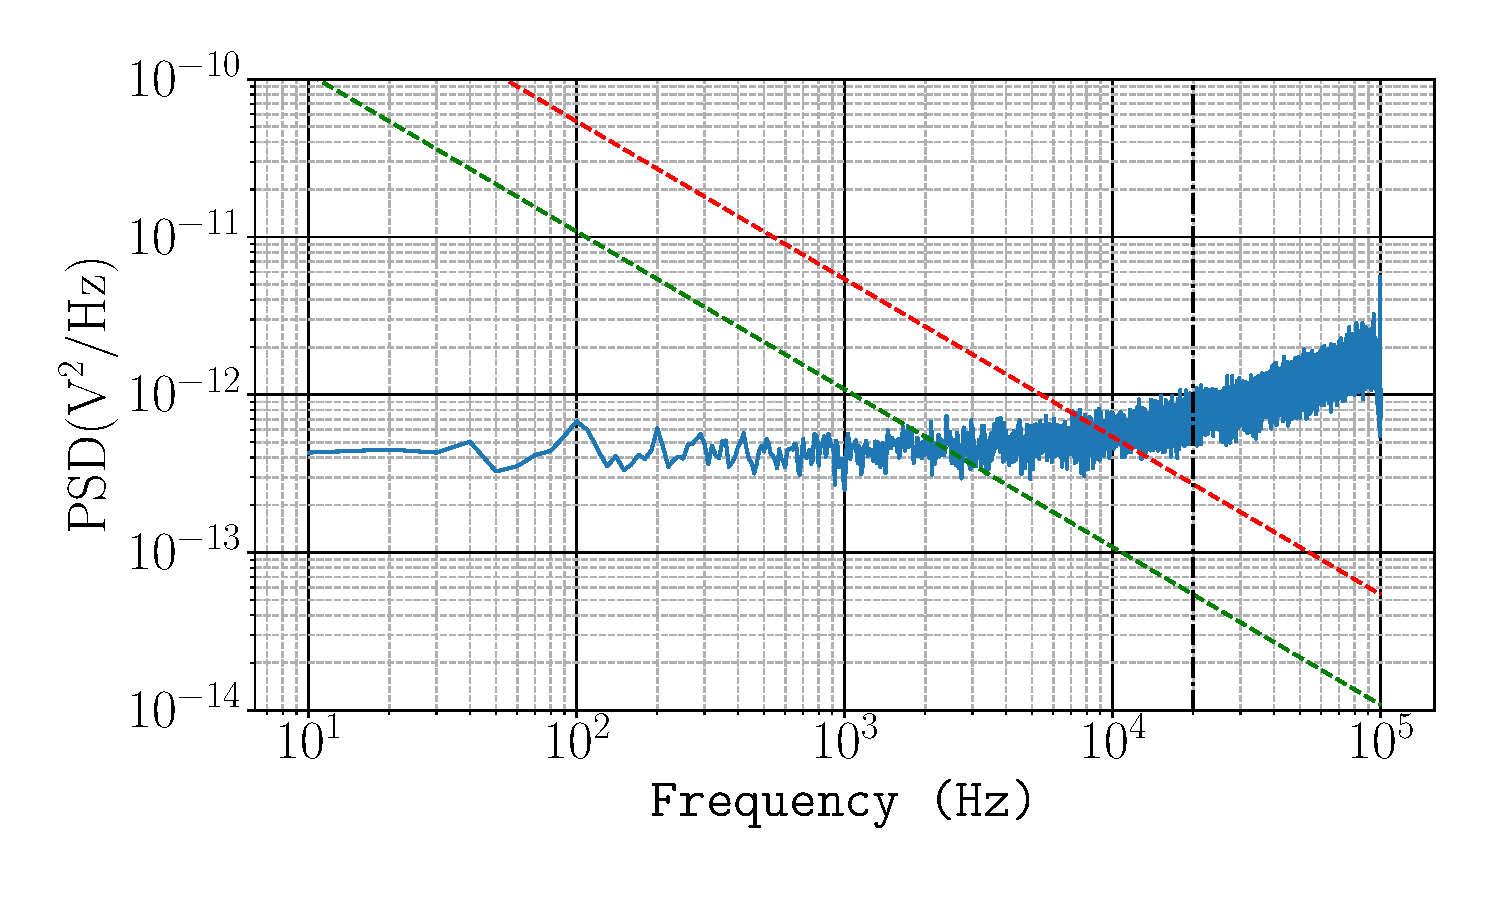
\includegraphics[width=0.7\textwidth]{noise_source_psd}
  \caption[Photodiode power spectral density]{Power spectral density
    of the voltage from the amplified photodiode signal
  sampled for \sivalue{2}{\second} at a rate of
\sivalue{200}{\kilo\hertz}. The red and green dashed lines indicate
the required voltage noise density to equal the quantum projection
noise level
after integrating for \(\tau = 2/f\)\sivalue{}{\s} for atom numbers of
\num{5e6} and \num{1e6}, respectively. The dot-dashed line indicates
the frequency corresponding to a detection time of
\sivalue{200}{\micro\s}.}
  \label{fig:noise_source_psd}
\end{figure}
%\par\noindent
%Averaging the detection signal over a time \(\tau\) has the effect of
%filtering the signal above the Nyquist frequency \(f_n = 1/(2 \tau)\).
%The variance in the averaged voltage over successive shots
%i.e. the Allan variance, is related to the power spectral density as
%follows
%\begin{equation}
%  \sigma^2_\text{av}(\tau) = 2 \int_0^\infty \frac{\sin(\pi \tau f)^4}{(\pi \tau f)^2}S(f)\;\mathrm{d}\;f
%  \label{eq:av_psd}
%\end{equation}
%Using~\EquationRef{eq:av_psd}, it is possible to determine the
%detection time required to reduce the shot-to-shot variance below the
%quantum projection noise level. \FigureRef{fig:detecion_av} shows the Allan deviation for increasing
%integration time. Above it shows the $\tau^{-1/2}$ dependence
%characteristic of uncorrelated white noise. The red and greed curves
%show the voltages corresponding to the quantum projection noise
%for the same numbers of atoms used
%in~\FigureRef{fig:noise_source_psd}. At the integration time of
%\sivalue{200}{\micro\second}, the detector noise
%is close to \sivalue{5}{\micro\volt} -- well below the quantum
%projection noise level.
%\begin{figure}[htpb!]
%  \centering
%  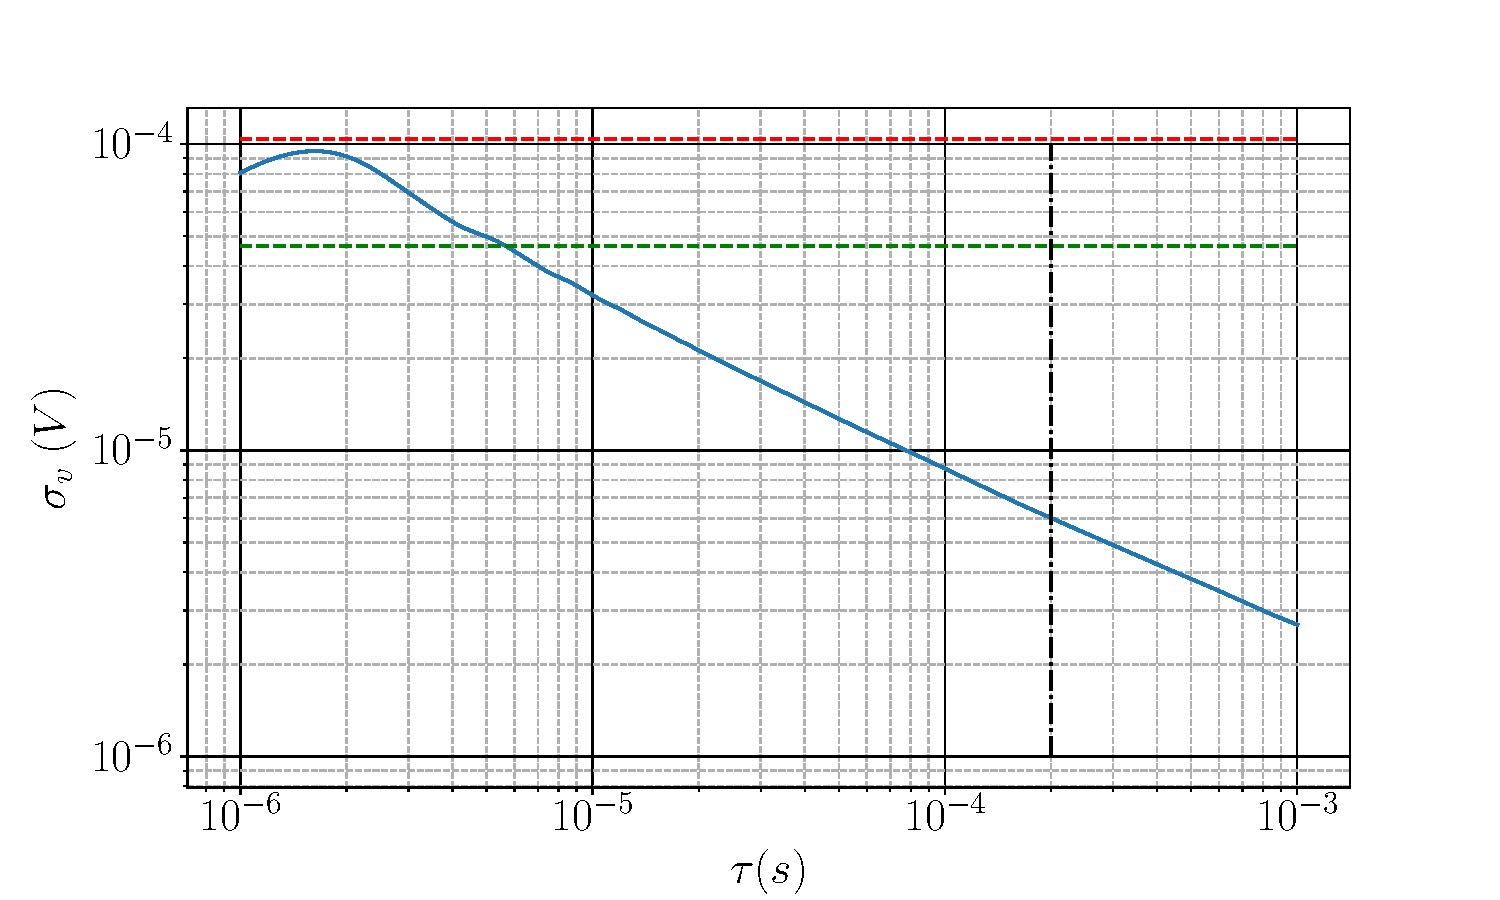
\includegraphics[width=0.7\textwidth]{detection_av}
%  \caption[Allan deviation of Photodiode voltage.]{Allan deviation of
%    the amplified photodiode voltages for increasing
%  integration time \(\tau\). The red and green dashed lines are the
%quantum projection noise levels for the atom numbers used
%in~\FigureRef{fig:noise_source_psd}. The black dot-dashed line indicates the
%integration time of \sivalue{200}{\micro\second} used in the
%experiment.}
%  \label{fig:detecion_av}
%\end{figure}

\subsubsection{Summary of Detection Noise}
It is worth summarising the various contributions to the noise in the
occupation probability $\text{P}_{\ket{F=2}}$. Fluctuations in the
atom number and detected photon number lead to shot noise
contributions to the voltages corresponding to $N_2$ and
$N_\text{Tot}$. However, we detect many photons per atom and in taking
the ratio of the two voltages, the contribution of variations in the
total atom number to $\text{P}_{\ket{F=2}}$ is largely suppressed.
This does not remove the quantum projection noise or technical noise
in the detector itself. Their effect on the interferometer uncertainty
are very different. The former represents a
fundamental limit to the measurement uncertainty, whereas the latter
is determined by the apparatus used in the experiment. In this case,
since the technical detector noise is greater than the projection
noise for the number of atoms in the experiment, the photodiode is
insufficiently sensitive and will need to be replaced by one with suitably
low noise.

\subsection{Acceleration Uncertainty}\label{subsec:accel_uncert}
The noise in measuring the occupation of each state determines the
accuracy to which the interferometer phase, and hence acceleration,
can be measured.
For simplicity, it is assumed that the fringe contrast $C$ is
independent from the mean probability of detecting atoms in
$\ket{F=2}$, $\text{P}_0$. This is valid if the contrast is reduced due to
inhomogeneities in the Rabi frequencies of each pulse and if the mean
probability is reduced from 0.5 by the presence of background $m_F=\pm
1$ atoms,
which can never occupy $\ket{F=2}$. Under these
assumptions~\EquationRef{eq:prob_measurement} yields the following variance
\begin{equation}
  \sigma_\text{P}^2 = \sigma_{P_0}^2 + \frac{1}{4} \sigma_C^2
  \cos(\Delta \Phi)^2 + \frac{C^2}{4}\sigma_{\Delta \Phi}^2 \sin(\Delta \Phi)^2
\end{equation}
At the mid-point of the fringe, $\Delta \Phi = \pi/2$, this variance
becomes
\begin{equation}
  \sigma_\text{P}^2 = \sigma_{P_0}^2 + 
  \frac{C}{4}\sigma_{\Delta \Phi}^2 
\end{equation}
so if $\text{P}_0$ and $C$ do not vary, the ratio of $\sigma_P$ to the
fringe amplitude $C/2$ is
given by
\begin{equation}
  S = \sigma_{\Delta \Phi}
\end{equation}
Returning to the interferometer sensitivity defined
in~\EquationRef{eq:sens_proj}, we can identify the maximum sensitivity
to accelerations as 
\begin{equation}
  \sigma_a = \frac{1}{\sqrt{n_{10}} k_\text{eff} T^2}
\end{equation}
So it is clear that the uncertainty in measuring the acceleration is enhanced by
increasing the number of atoms or by increasing the time between
interferometer pulses. Of course, this is an under-estimate as other sources of noise will result in a
greater uncertainty. Nevertheless, it provides a useful
figure-of-merit for quantifying other sources of noise in terms of
their equivalent acceleration uncertainty. 

\subsection{The Allan Variance}\label{subsec:allan_variance}
The variance of successive measurements is often a useful measure for
quantifying uncertainty. However with a finite sequence
of measurements, this depends on the number of samples and might not
converge as the number of samples increases. On the other hand, the
two-sample variance 
\begin{equation}
  \sigma^2(\tau) = \frac{1}{2}\left\langle
  (a_{n+1}-a_n)^2\right\rangle
  \label{eq:two_sample_var}
\end{equation}
does not depend on the number of samples. This can be generalized to
longer time separations \(t = N \tau\) by taking the mean of \(N\)
consecutive measurements
\begin{equation}
  \sigma_\text{av}^2(t) = \frac{1}{2}
  \left\langle
  \left(\frac{1}{N}\sum_{k=0}^{N-1}a_{n+1}-\frac{1}{N}\sum_{k=N}^{2N-1}a_n\right)^2\right\rangle
  \label{eq:allan_var_mean}
\end{equation}
which is referred to as the Allan variance~\cite{Allan1966}. Operationally, the Allan variance is useful for characterising the
correlation of measurement noise. 
%For instance, in the case of white
%noise, the uncertainty in each measurement is uncorrelated
%and the Allan variance becomes
%\begin{equation}
%  \sigma^2_\text{av}(t) = \frac{1}{N}\sigma^2_\text{av}(\tau)
%\label{eq:allan_var_simp}
%\end{equation}
%This is typically the case over short timescales. More generally, the
The Allan variance can be used to identify the timescales that
characterise the behaviour of the bias in an
accelerometer~\cite{El-Sheimy2008}. At short
timescales, the Allan variance is dominated by white noise if the
uncertainty in successive measurements is uncorrelated. 
At longer timescales the bias instability -- fluctuations of
the bias value -- causes the Allan variance to reach a minimum value.
Finally, at still longer timescales, the bias drift -- a long-term
change in the bias value -- causes
an increase in the Allan variance. \TableRef{tab:avar} summarises these three processes and their characteristic dependences on $\tau$. 
\begin{table}[htpb]
  \centering
  \begin{tabular}{cc}
  \toprule
    Process & $\tau$ dependence \\ 
    \midrule
    White noise & $\tau^{-1}$ \\
    Bias instability & $\tau^{0}$ \\
    Bias drift & $\tau^{2}$\\
    \bottomrule
  \end{tabular}
  \caption{Allan variance characteristic timescales.}
  \label{tab:avar}
\end{table}

\subsection{The Sensitivity Function}\label{subsec:sens_func}
The sources of noise presented thus far arise from statistical
uncertainties in measuring the number of atoms and are not present in
the ideal case of perfect interferometer contrast. However, there are
still other sources which introduce interferometer phase noise. Generally speaking, these add a random component to
the interferometer phase which is independent of the forces acting on
the atoms. Two dominant sources of phase noise are vibrations of the
retro-reflecting mirror and laser phase noise, i.e. fluctuations in
the relative phase between the two Raman light
fields~\cite{Cheinet2008}.
\par\noindent
The sensitivity function~\cite{Dick1987}
defines the instantaneous shift of the
interferometer phase \(\delta\Phi\) at a time \(t\) due to a phase
shift of the Raman laser phase \(\delta \phi\)
\begin{equation}
  g(t) = \lim_{\delta\phi \rightarrow 0} \frac{\delta\Phi(\delta \phi,
  t)}{\delta(\phi)}
  \label{eq:sensitivity_def}
\end{equation}
so the interferometer phase shift induced by fluctuations of
\(\phi\) is given by
\begin{align}
  \Phi &= \int_{-\infty}^\infty g(t)\delta \phi\;\mathrm{d}\phi(t)
  \nonumber\\
  &= \int_{-\infty}^\infty g(t)\;\frac{\mathrm{d}\phi}{\mathrm{d} t}\;
  \mathrm{d}t
  \label{eq:phase_contrib}
\end{align}
In the case of a \(\pi/2-\pi-\pi/2\) interferometer pulse sequence of
durations \(\tau_R-2 \tau_R - \tau_R\) and where \(t=0\) is defined at
the centre of the \(\pi\) pulse, the sensitivity function is 
\begin{equation}
    g(t) = 
    \begin{cases}
      \sin ( \Omega t) & 0<t<\tau_R  \\
      1 & \tau_R <t<\tau_R +T \\
      \sin (\Omega  (t-T)) & \tau_R +T<t<2 \tau_R +T
  \end{cases}
\label{eq:sensitivity_interferometer}
\end{equation}
for a pulse separation time \(T\).  
\subsection{Influence of Laser Phase Noise}\label{subsec:laser_phase}
The response of the interferometer phase to laser phase noise is
best understood in the frequency domain. In particular, the inverse
of the interferometer pulse separation time 
The effects of \(\phi\) are best
thought of in terms of its Fourier components. Writing \(\phi(t) = A
\cos(\omega t + \psi)\), \EquationRef{eq:phase_contrib} becomes
\begin{equation}
  \Phi = - A \omega \cos(\psi) \int_{-\infty}^\infty g(t) \sin(\omega
  t) \mathrm{d} t
  \label{eq:phase_fourier}
\end{equation}
where the term proportional to \(\cos(\omega t)\) has been dropped,
since \(g(t)\) is an odd function. The integrand
in~\EquationRef{eq:phase_fourier} is proportional to the Fourier
transform of \(g(t)\)
\begin{equation}
  G(\omega) = -i \int_{-\infty}^{\infty} g(t) \sin(\omega t)
  \mathrm{d} t
  \label{eq:sensitvity_fourier}
\end{equation}
which using~\EquationRef{eq:sensitivity_interferometer}
becomes~\cite{Canuel2007}
\begin{equation}
  G(\omega) = \frac{4 i
  \Omega}{\omega^2-\Omega^2}\sin\left(\frac{\omega(T+2\tau)}{2}\right)\left(\cos\left(\frac{\omega(T+2\tau)}{2}\right)
  + \frac{\omega T}{2}\sin \left(\frac{\omega T}{2}\right)\right)
  \label{eq:sens_fourier_full}
\end{equation}
so~\EquationRef{eq:phase_contrib} becomes
\begin{align}
  \Phi &= -i A \cos(\psi) \;\omega G(\omega) \nonumber \\
  &= - A \cos(\psi) \lvert H(\omega)\rvert
  \label{eq:interfometer_fourier}
\end{align}
\par\noindent
A plot of the transfer function \(|H(\omega)|^2\) is presented
in~\FigureRef{fig:transfer_function} for
\(T= \)\sivalue{20}{\milli\second} and \(\tau
= \)\sivalue{20}{\micro\second}. The asymptotic properties of the
transfer function can be summarised as follows:
\begin{itemize}
  \item At low frequencies \(\omega \ll \Omega\), the transfer
    function is approximated by 
    \begin{equation}
      |H(\omega)|^2 \approx 16 \sin \left(\frac{\omega T}{2}\right)^4
    \end{equation}
    which is a periodic function that is zero at frequency multiples
    of \(1/\pi T\) \\
  \item At frequencies \(\omega \gg \Omega\), the transfer function is
    \begin{equation}
      |H(\omega)|^2 \approx 4 \frac{\Omega^2}{\omega^2}\sin
      \left(\omega T\right)^2
    \end{equation}
    which is zero at multiples of \(1/2\pi T\) and is a low-pass
    first-order filter.
\end{itemize}
\begin{figure}[htpb!]
  \centering
  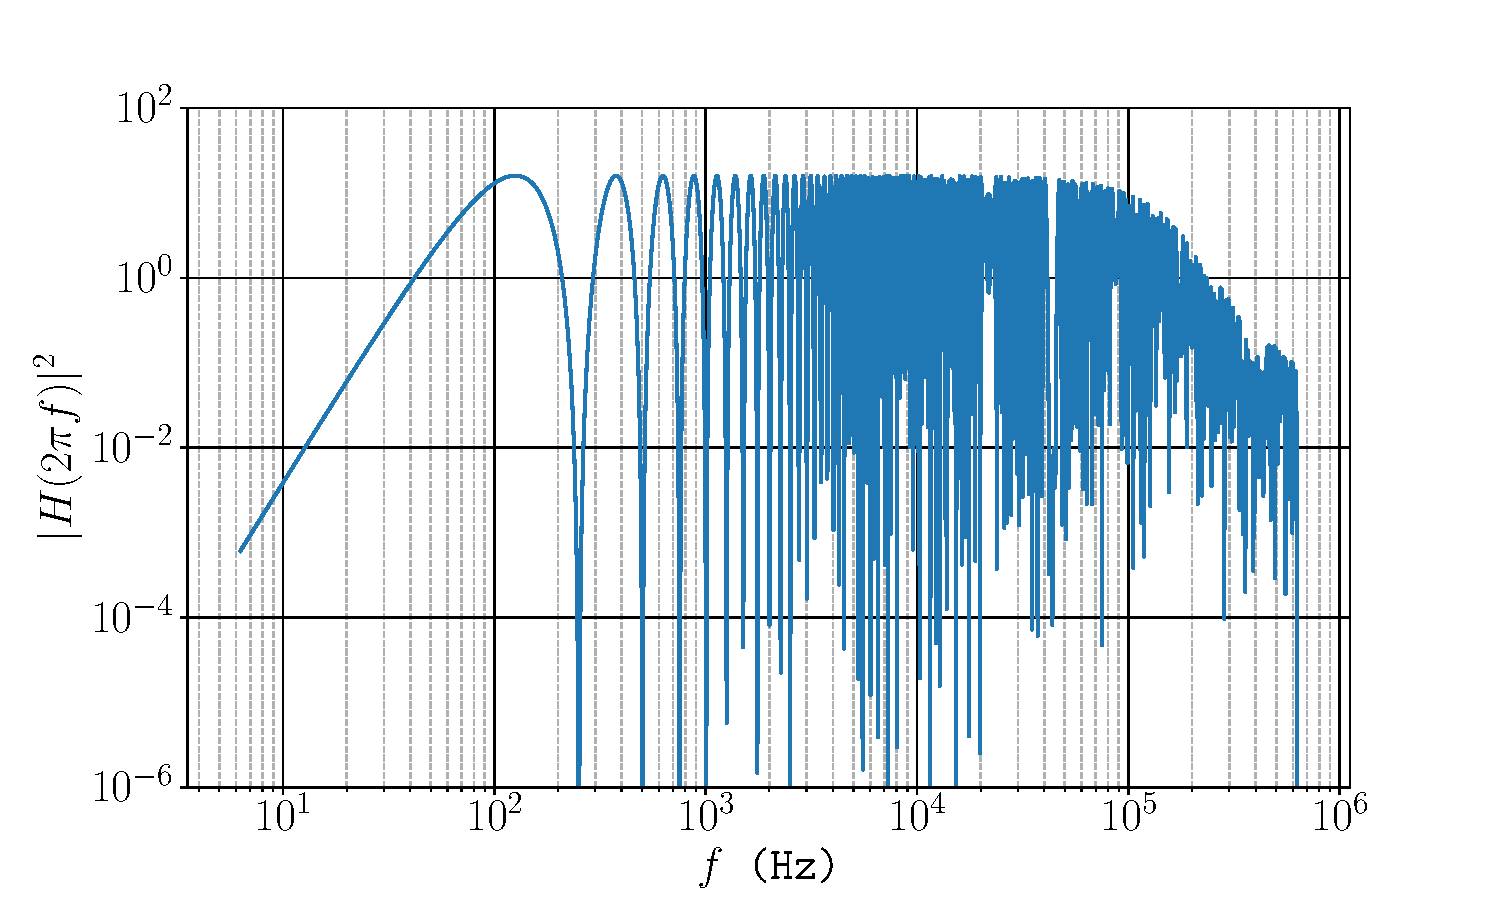
\includegraphics[width=0.7\textwidth]{transfer_func_laser.pdf}
  \caption[Transfer function for laser phase noise.]{Transfer function
  for laser phase noise. Here, the separation between pulses is \(T =
  \)\sivalue{20}{\milli\second} and the \(\pi/2\) pulse time is \(\tau
=\)\sivalue{20}{\micro\second}.}
  \label{fig:transfer_function}
\end{figure}
\par\noindent
The variance of \(\Phi\) is obtained by averaging over \(\psi\)
\begin{equation} 
  \sigma_\Phi^2 = \langle \Phi^2\rangle_\psi = \frac{1}{2} A^2
  |H(\omega)|^2
  \label{eq:var_phi_transfer}
\end{equation} which is related to the phase noise power spectral density
\(S_\phi(\omega)\) by
  \begin{equation}
    \sigma_\Phi^2 = \frac{1}{2}\int_{-\infty}^\infty
    S_\Phi(\omega)|H(\omega)|^2 \frac{\mathrm{d}\omega}{2\pi} =
      \int_0^\infty
    S_\Phi(\omega)|H(\omega)|^2 \frac{\mathrm{d}\omega}{2\pi} 
    \label{eq:phase_noise_psd}
  \end{equation}
Similarly, the Allan variance can be expressed using the transfer
function and the phase noise power spectral density~\cite{Gouet2008}.
The integration time \(\tau_\text{av} = m T_c\) is expressed in multiples
of the experiment cycling time \(T_c\). In the frequency domain, the phase
noise power spectral density is sampled at frequency multiples of
\(f_c = 1/T_c\), so the Allan variance becomes
\begin{equation}
  \sigma^2_\Phi(\tau_\text{av}) = \frac{1}{\tau_\text{av}}
    \sum_{k=1}^\infty |H(2\pi k f_c|)^2S_\phi(2\pi k f_c)
  \label{eq:avar_transfer}
\end{equation}
\par\noindent
The laser phase noise originates from the reference oscillator used in
the phase-locked loop for the M-Squared laser. The phase noise
spectral density and corresponding Allan deviation for increasing
integration time was measured by M-Squared during installation of the
laser system. A plot of the Allan deviation is shown
in~\FigureRef{fig:allan_dev_m2}. At an interferometer pulse
separation of
\(T = \) \sivalue{25}{\milli\second}, the phase noise in the Raman
laser results in an uncertainty in the interferometer phase of
\sivalue{10}{\milli\radian}. 
\begin{figure}[htpb!]
  \centering
  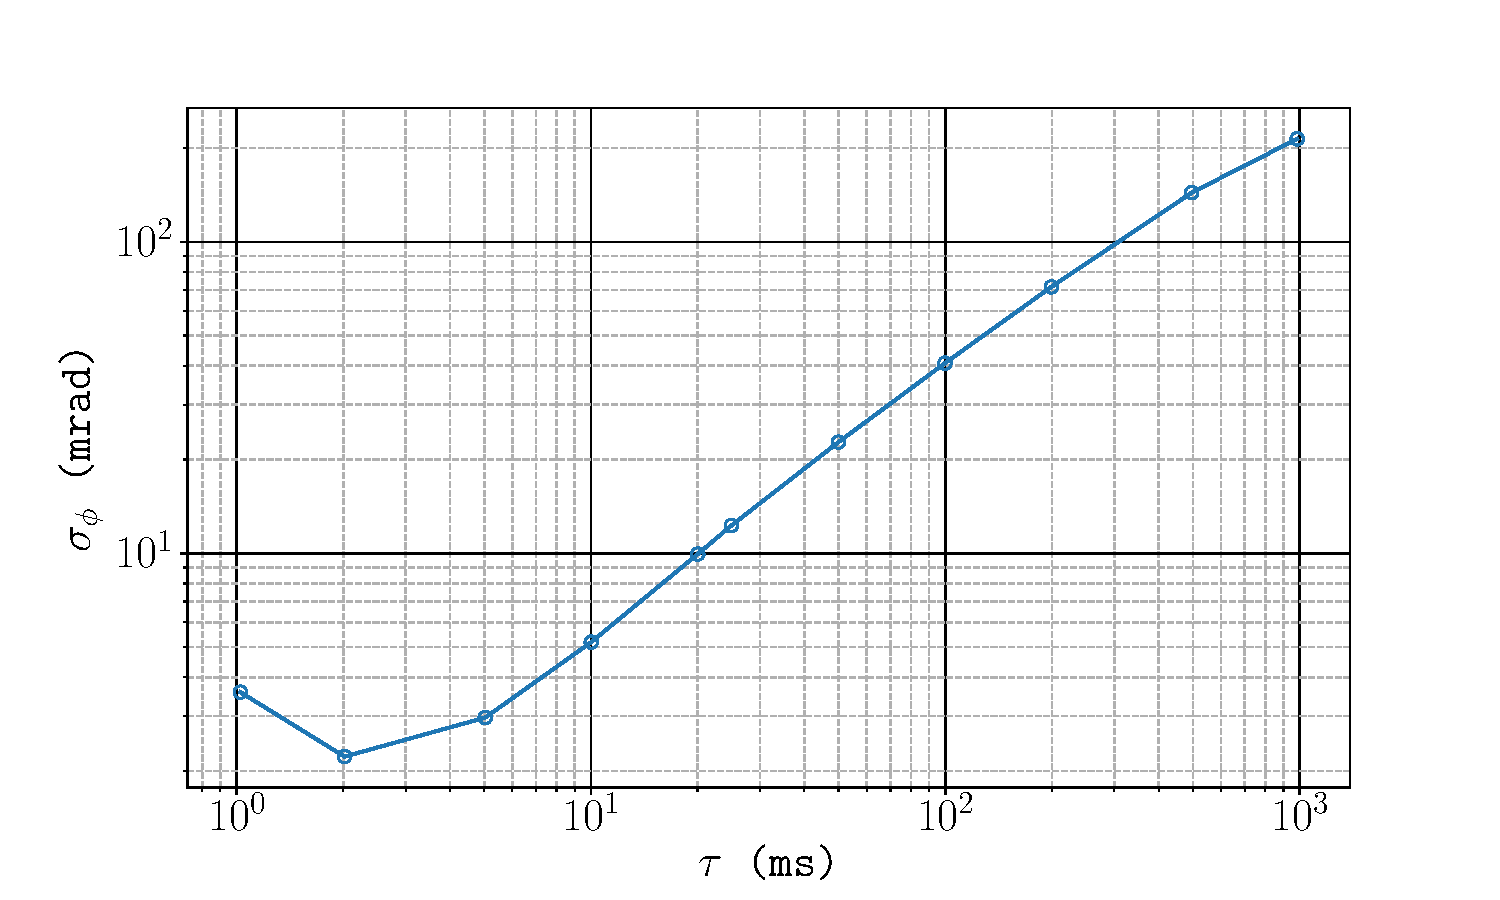
\includegraphics[width=0.7\textwidth]{allan_dev_m2.pdf}
  \caption[Allan deviation of the Raman laser phase difference.]{Allan deviation of the Raman laser phase difference for increasing integration time. Data reproduced from~\cite{M2_manual}.}
  \label{fig:allan_dev_m2}
\end{figure}


\subsection{Vibrations}\label{subsec:vibration_noise}
The phase difference between the two Raman beams depends on the
position of the retro-reflecting mirror. Consequently, this defines a frame of
reference for the position of the atoms during the interferometer. Any
random motion of the mirror, for instance from mechanical vibrations,
introduces a random component to the laser phase~\cite{Vigue2006}. An acceleration of
the mirror modifies the laser phase as follows
\begin{equation}
  \frac{\mathrm{d}^2 \Phi(t)}{\mathrm{d} t^2} = \keff.\textbf{a}(t)
  \label{eq:phase_acc}
\end{equation}
and the sensitivity to accelerations \(g_a\) is given by
\begin{equation}
  \frac{1}{k_\text{eff}} \frac{\mathrm{d}^2 g_a(t)}{\mathrm{d} t^2} =
  g(t) \\
  \label{eq:acc_sens}
\end{equation}
Assuming that the pulse time \(\tau\) is much shorter than the
interferometer pulse separation, \(T\), the acceleration sensitivity
function is approximated by
\begin{equation}
  g_a(t) = \begin{cases}
 -1 & - T < t < 0\\
 1 & 0 < t < T
  \end{cases}
  \label{eq:acc_sens_approx}
\end{equation}
From this, the acceleration transfer function is
\begin{equation}
  |H_a(\omega)|^2 = \frac{k_\text{eff}^2}{\omega^2}|H(\omega)|^2 
  \label{eq:acc_transfer}
\end{equation}
which in the low frequency limit \(\omega \ll \Omega\) is
\begin{equation}
  |H_a(\omega)|^2 = \frac{16 k_\text{eff}^2}{\omega^4}
  \sin\left(\frac{\omega T}{2}\right)^4
  \label{eq:acc_tf_low}
\end{equation}
Equivalent definitions for the variance and Allan variance are
obtained using this and the acceleration noise spectral density
\(S_a(2\pi f)\) as the respective definitions
in~\EquationRef{eq:phase_noise_psd}
and~\EquationRef{eq:avar_transfer}. \FigureRef{fig:transfer_func_acc}
shows the transfer function for
acceleration noise is shown in. The
gain is largest at low frequencies and approximates a second-order
filter at higher frequencies.
\begin{figure}[htpb]
  \centering
  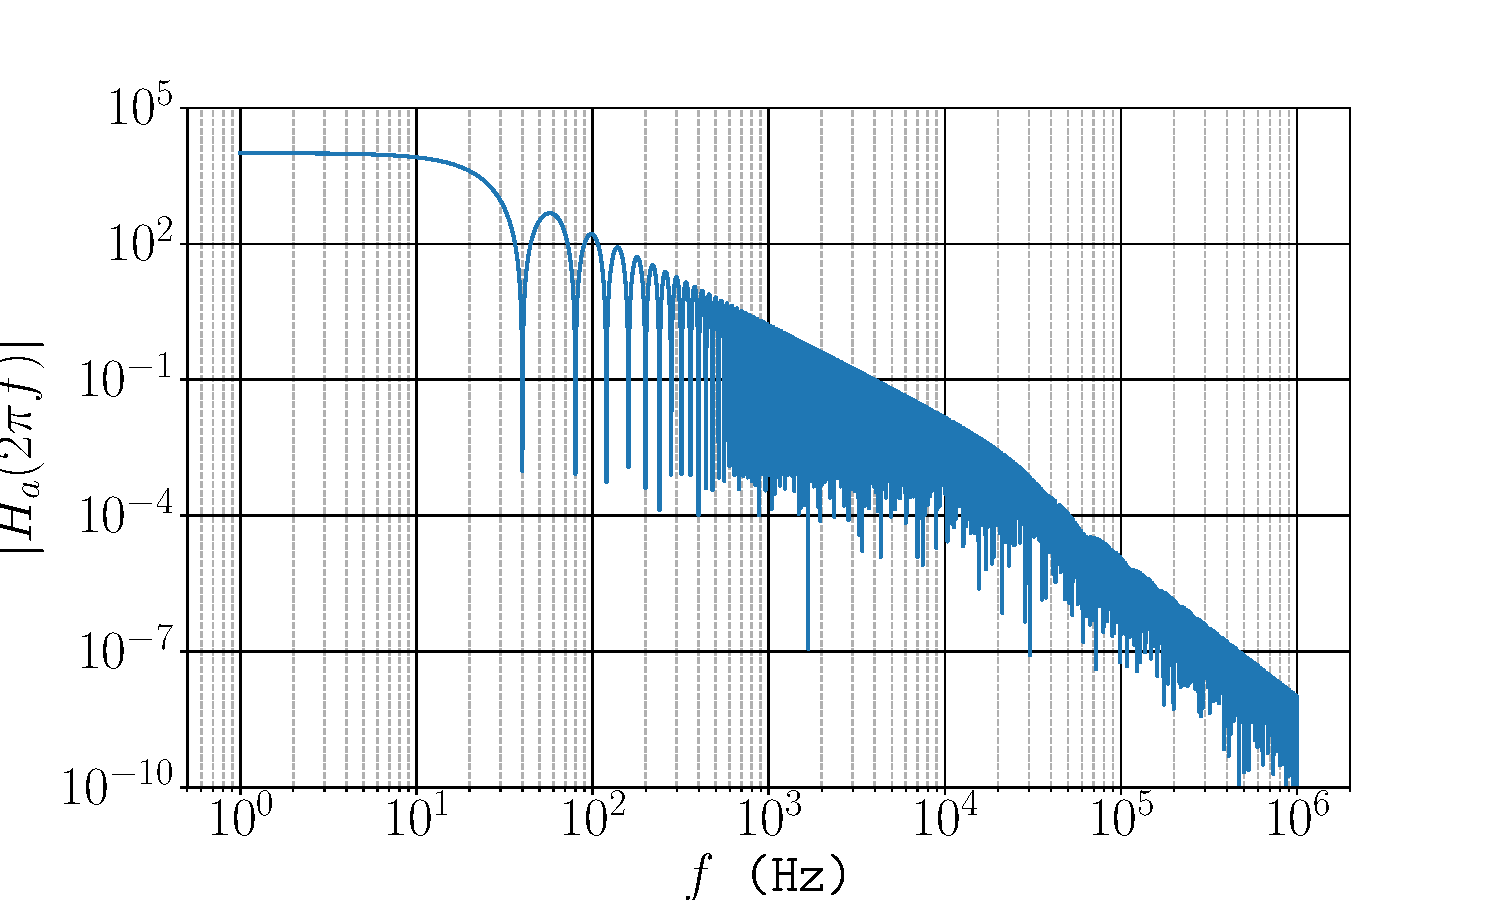
\includegraphics[width=0.7\textwidth]{transfer_func_acc}
  \caption[Acceleration noise transfer function.]{Acceleration noise
  transfer function. The parameters used here are the same as those
previously defined for~\FigureRef{fig:transfer_function}.}
  \label{fig:transfer_func_acc}
\end{figure}
\subsubsection{Measuring the Acceleration Noise Power Spectral Density}
The interferometer phase is most sensitive to low-frequency
vibrations. Acceleration noise at frequencies greater than \(1/2T\)
will mostly average out, contributing little to an overall phase.
Precise measurements of the interferometer phase rely on reducing the
low frequency noise. The vibration of the retro-reflecting mirror is
reduced by passively isolating it from its environment. The
chamber is mounted on a layer of Sorbothane to dissipate
vibrations from the ground. This isolation is enhanced by a
pneumatic suspension system between the optical table and its
supporting legs. 
\par\noindent
\FigureRef{fig:vibration_spectrum} shows a comparison of the acceleration noise spectral density with and
without the pneumatic suspension, measured using
the accelerometer mounted behind the retro-reflecting mirror. The suspension acts as a
low-pass filter and reduces the power within the
10-\sivalue{200}{\hertz} bandwidth, which is aliased into the lower
frequency band. For an interferometer pulse separation of \(T =
\) \sivalue{25}{\ms}, the
vibration phase noise using~\EquationRef{eq:avar_transfer} is \(\sigma_\Phi =\) \sivalue{270}{\milli\radian}. Without
floating the table, this becomes \sivalue{7}{\radian}. This is the dominant
source of phase noise using the current vibration isolation systems.
This phase noise can be reduced using more sophisticated method of damping vibrations, such as an active
isolation system~\cite{Zhou2012}.
\begin{figure}[htpb!]
  \centering
  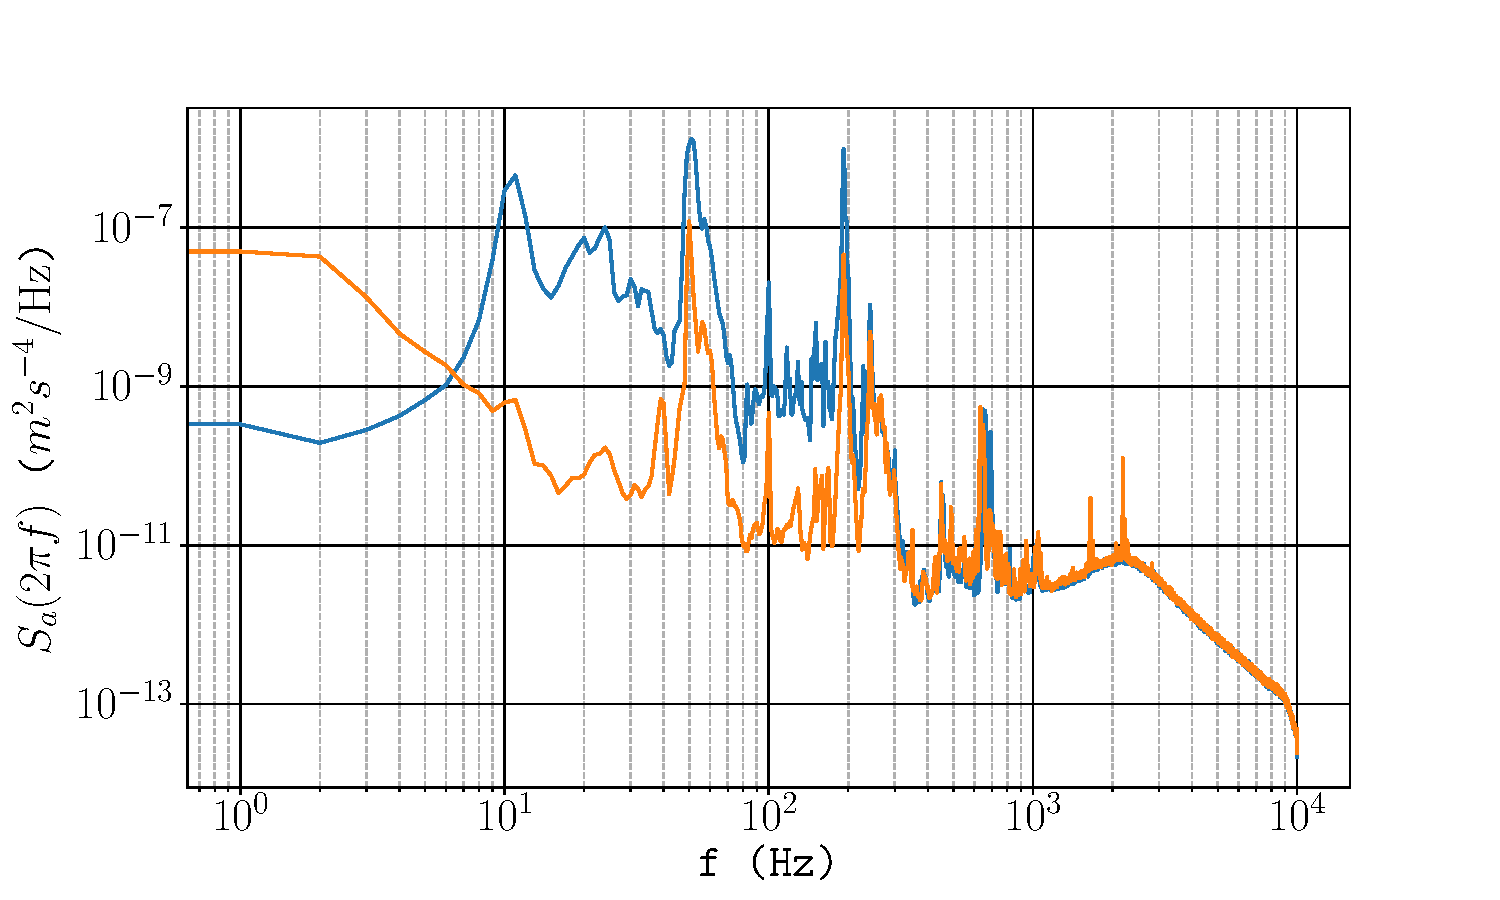
\includegraphics[width=0.7\textwidth]{vibration_spectrum.pdf}
  \caption[Acceleration noise power spectral density.]{Acceleration
  noise power spectral density sampled at a rate of
\sivalue{20}{\kilo\hertz}. The orange curve shows the acceleration
power spectral density using pneumatic suspension to decrease the
coupling of vibrations from the ground to the experiment. For
comparison, the blue curve shows the power spectral density without
this isolation.}
  \label{fig:vibration_spectrum}
\end{figure}
%\subsection{Other Sources of Phase Noise}
%Aside from laser phase noise and vibrations, there are additional effects
%which result in interferometer phase noise. These have not been
%characterised in this experiment as their magnitude is typically much
%smaller than the present vibration phase noise. 
%\begin{itemize}
%  \item \underline{Magnetic field gradients}. The \(\Delta_m = 0\)
%    clock transition has a second-order Zeeman shift of
%    \sivalue{575}{\Hz\gauss\tothe{-2}}. A gradient of magnetic field
%    across the area traversed by the atoms introduces a propagation
%    phase which does not cancel. 
%  \item \underline{Laser intensity noise}.
%\end{itemize}
\subsection{Summary of Identified Noise Sources}\label{subsec:noise_sources}
To conclude this discussion, it is helpful to compare the identified
sources of noise. These are not a complete list of the effects which
reduce the sensitivity to accelerations, but are the most dominant. The
identified sources and their estimated effects on acceleration
measurements are shown in~\TableRef{tab:noise_sources}. The largest
contributor comes from vibrations of the retro-reflecting mirror.
Other noise sources, such as magnetic field gradients, laser intensity
noise and rotations have not yet been characterised. Higher-order
phase shifts due to inertial effects, such as the Coriolis force and
gravity gradients, have been
studied elsewhere\cite{Bongs2006}.
\begin{table}[htpb!]
  \centering
  \begin{tabular}{ccc}
    \toprule
    Noise Source & Signal/Noise & \(\sigma_a\)
    (\sivalue{}{\micro\meter\per\s\squared}) \\
    \midrule
    Projection noise (\num{5e6} atoms) & 2200 & 0.07 \\
    Laser phase noise & 157 & 1 \\
    Technical detector noise & 15 & 10.5 \\
    Vibrations & 5.8 & 26\\
    \bottomrule
  \end{tabular}
  \caption[Comparison of known noise sources.]{Comparison of known noise sources and their effects on
  acceleration measurements. These values are estimated assuming a
separation between pulses of \(T = \)\sivalue{25}{\ms} and a \(\pi/2\)
pulse time of \(\tau = \)\sivalue{20}{\micro\s}.}
  \label{tab:noise_sources}
\end{table}
\section{Measuring Accelerations}\label{sec:atomint_accelerations}
This section presents the techniques used to characterise the atom interferometer
and its sensitivity to accelerations. It begins with a calibration of
the fringe pattern in~\SectionRef{sec:fringe_cal}. Following this, a
method for filtering the effects of vibrations is given
in~\SectionRef{sec:vibration_senstivity}. This section concludes with
a measurement of the Allan variance to determine the long-term
stability in~\SectionRef{subsec:stability}.
\subsection{Fringe Calibration}\label{sec:fringe_cal}
With spatial resolution of the atom cloud, it is possible to resolve
the fringe contrast from a single shot~\cite{Sugarbaker2013}. Of
course, this is not possible using a photodiode, so the fringe
contrast is measured using successive experiment
cycles~\cite{Peters2001}. 
The interferometer phase difference $\Delta \Phi$ is controlled 
by varying the phase difference between the two Raman lasers for the
middle \(\pi\) pulse. Since \(\Delta \Phi = \phi_1 - 2\phi_2
+\phi_3\), varying \(\phi_2\) induces the largest change in
\(\Delta\Phi\). \FigureRef{fig:fringe_examp} shows an interference fringe obtained in this
manner. In this instance, the contrast is \(C = 0.055\) and the mean
probability of detecting in \(\ket{F=2}\) is \(\textnormal{P}_0 =
0.39\).
\begin{figure}[htpb!]
  \centering
  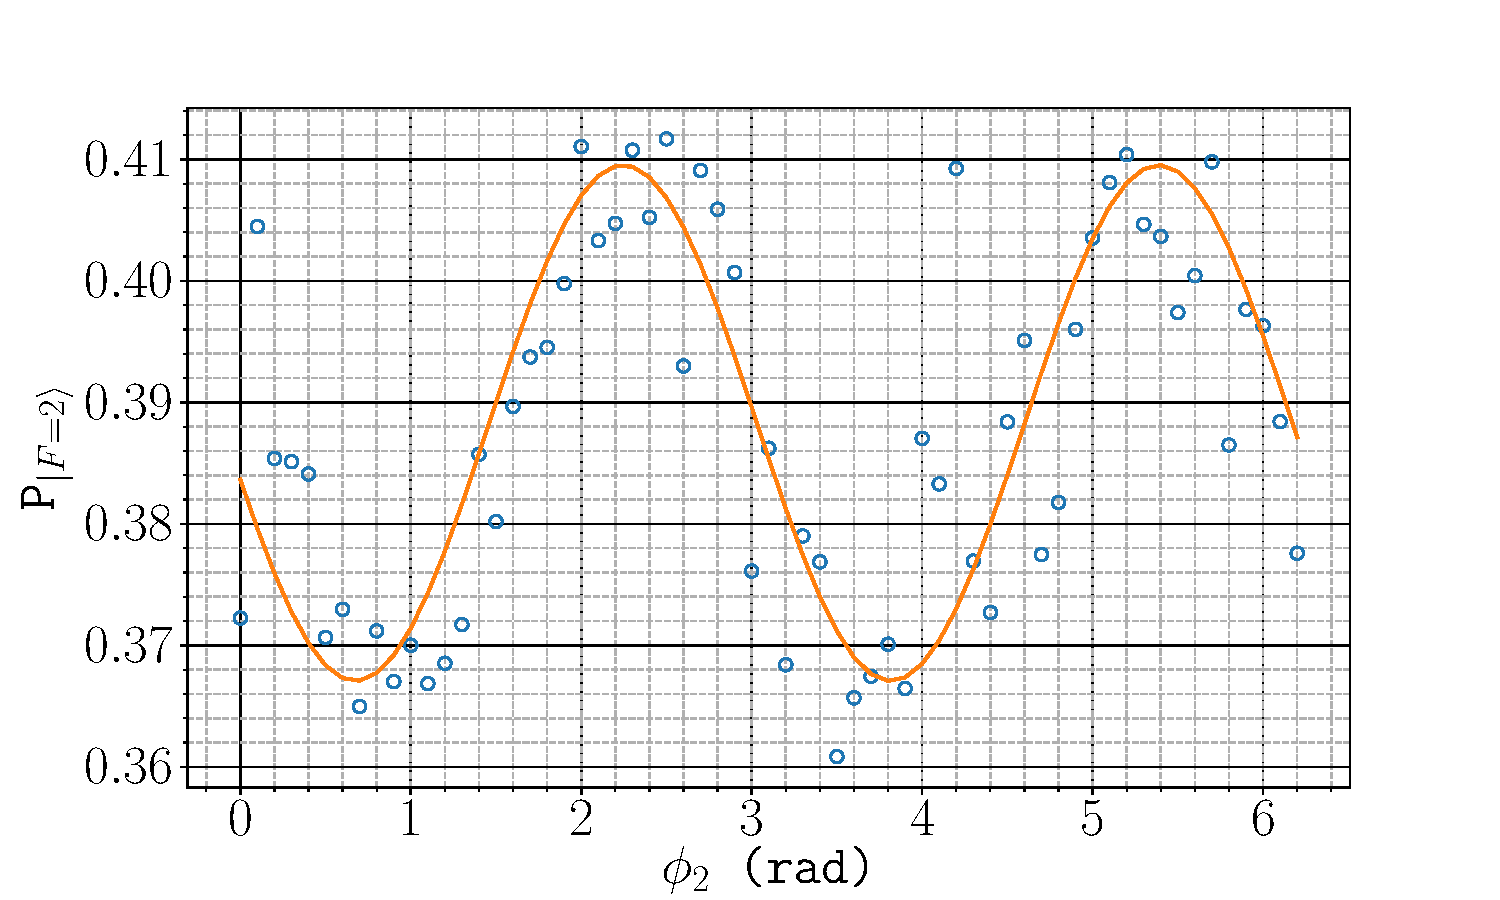
\includegraphics[width=0.7\textwidth]{fringe_examp}
  \caption[Interference fringe for \(T = \)\sivalue{25}{\ms}.]{Interference fringe obtained by varying the phase
    difference of the two Raman lasers during the middle \(\pi\) pulse
    for a pulse separation time of \(T = \)\sivalue{25}{\ms}. The orange
curve is a non-linear least squares fit to the data, giving a contrast
of \(C = 0.055\) and a mean value of \(\textnormal{P}_0 = 0.39\). The
shaded region indicates the 95\% confidence band. }
  \label{fig:fringe_examp}
\end{figure}

\subsection{Correcting for Vibration
Noise}\label{subsec:vibration_sensitivity}
Vibrations of the retro-reflecting mirror are a significant source of
phase noise, which limits the sensitivity of the interferometer to
accelerations. This is particularly apparent when the vibration noise
induces a phase shift of greater than 2\(\pi\) radians. If the
interferometer signal spans multiple fringes, it is not possible to
accurately determine acceleration from the phase shift.
\par\noindent
One method to filter the effects of vibration noise, described in
~\cite{Merlet2009}, uses the MEMS accelerometer to measure the
vibration of the retro-reflecting mirror between the
first and last interferometer pulse. After this time, the phase shift
due to vibrations is given by the following convolution
\begin{equation}
  \phi_\textnormal{vib} =  \keff T^2 K\int_{-T}^{T} g_a (t) V(t)
  \mathrm{d}t = \keff T^2 K
  \widetilde{V}_\textnormal{vib}
  \label{eq:phase_vib}
\end{equation}
where \(V(t)\) is the voltage measured across the output of the MEMS
accelerometer, \(K = \) \sivalue{0.793}{\m\s\tothe{2}\per\V} is the
scaling factor from voltage to acceleration and \(g_a(t)\) is the
acceleration sensitivity function, defined
in~\EquationRef{eq:acc_sens_approx}. Leaving the scaling factor as a
free parameter $\alpha$, the interferometer signal is
fit to the function
\begin{equation}
  \text{P}_{\ket{F=2}} = \text{P}_0 + \frac{C}{2}\sin(\alpha
  \widetilde{V}_\textnormal{vib} + \phi_0)
  \label{eq:fringe_fit_vibration}
\end{equation}
\par\noindent
Common-mode suppression of the vibration phase noise is achieved by
estimating the interferometer phase from the residuals of the fit
to~\EquationRef{eq:fringe_fit_vibration}. If the interferometer phase
as estimated from~\EquationRef{eq:interferometer_phase} is denoted
\(\phi_\textnormal{int}\), then the fit residuals are
\(\phi_\textnormal{res} =  \phi_\textnormal{int} -
\phi_\textnormal{vib}\).
The correlation of the acceleration measured by the MEMS accelerometer
and the interferometer signal is shown
in~\FigureRef{fig:vib_comparison}. The Raman laser phase difference was
initially set so that the interferometer signal was at the mid-point
of the fringe \(\Delta \phi = \pi/2\) before continuously running the
experiment. The vibration noise was increased
by removing the pneumatic suspension of the optical table, which
helps to passively isolate the experiment from external vibrations
that are coupled through the table legs. Without this additional
suppression, the vibration noise is large enough to shift the
interferometer phase by more than \(2\pi\), as indicated
in~\FigureRef{fig:high_vib}. When the table is suspended, the
vibration noise is small enough that the interferometer signal remains
on one side of the fringe.
\begin{figure}[htpb!]
  \centering
  \subfloat[][]{\scalebox{0.5}{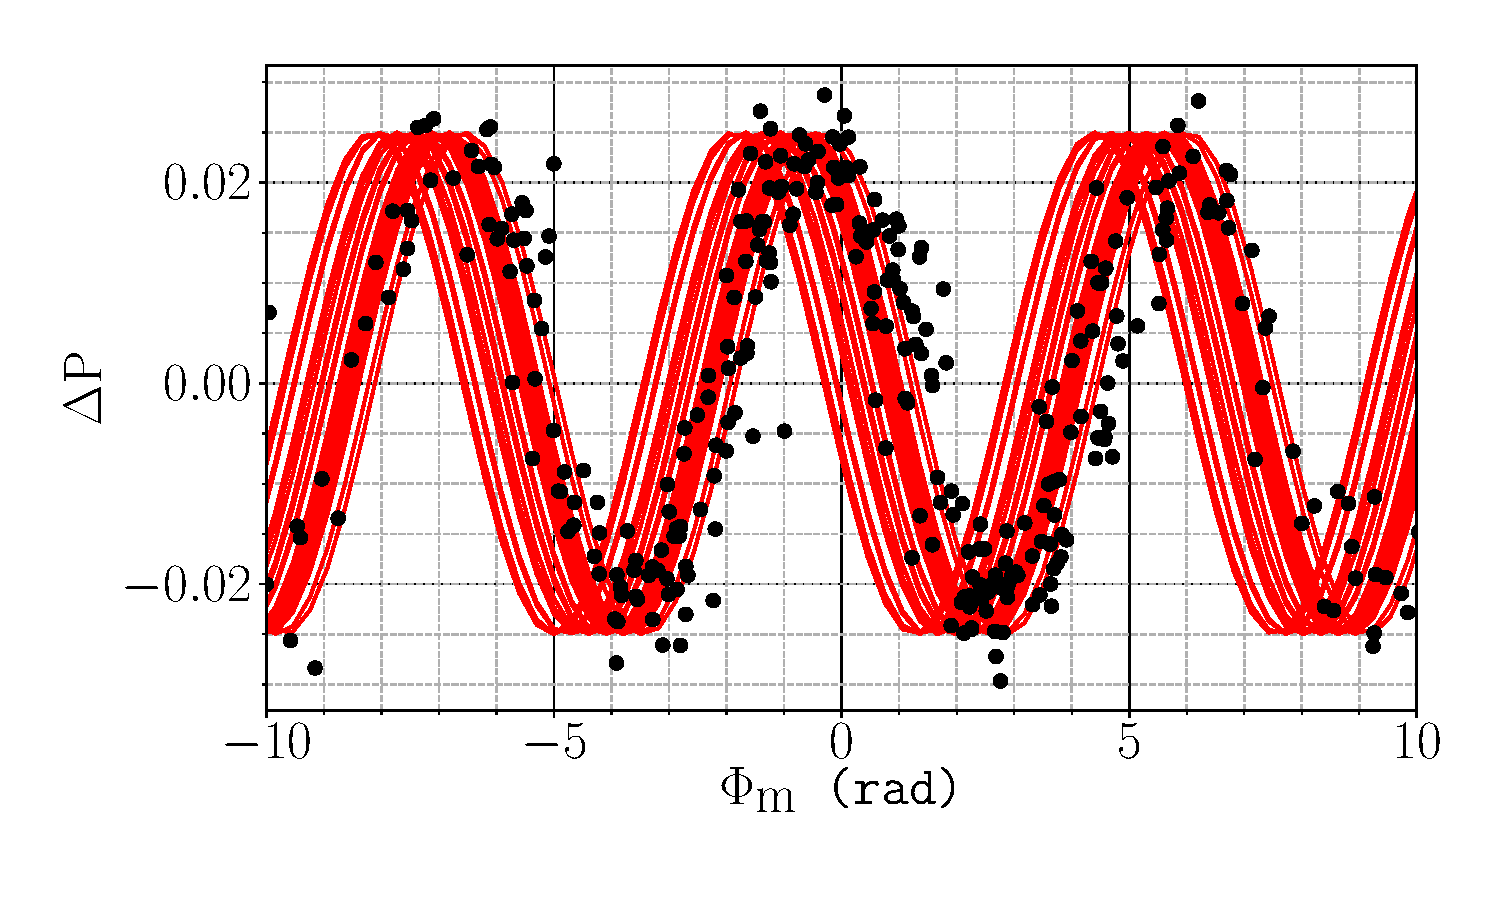
\includegraphics{high_vib}}\label{fig:high_vib}}
    \subfloat[][]{\scalebox{0.5}{\includegraphics{low_vib}}\label{fig:low_vib}}
  \caption[Comparison of MEMS/Interferometer correlation in a high and
    low vibration
  environments.]{Correlation between acceleration measured by the MEMS
    accelerometer and the interferometer signal. \textbf{(a)} shows
    the correlation measured in high vibration environment, when the
    optical table was not pneumatically suspended. \textbf{(b)} shows
    the reduction in phase noise with this additional vibration
  isolation.}
  \label{fig:vib_comparison}
\end{figure}
\par\noindent
The suppression of the vibration noise can be seen in the distribution
of the estimated acceleration. \FigureRef{fig:vibration_hists} shows
histograms of the acceleration measured by the MEMS and the
interferometer in the low vibration instance
of~\FigureRef{fig:low_vib}. \FigureRef{fig:low_vib_hist_mems_atom} compares the distribution of
the accelerations measured by the MEMS with that of the
interferometer. The noise in the MEMS signal is larger than in the
interferometer -- their respective standard deviations are
$\sigma_a^{(m)} =$ \sivalue{66.8}{\um \s\tothe{-2}} and
$\sigma_a^{(i)} =$ \sivalue{20.8}{\um \s\tothe{-2}}. The MEMS
accelerometer has a higher acceleration bandwidth (\sivalue{20}{\kHz}) than the
interferometer (\sivalue{20}{\Hz}). Consequently, the interferometer
is not sensitive to the high-frequency noise measured by the MEMS
accelerometer. \FigureRef{fig:low_vib_hist_atom_res} compares the acceleration noise
from the interferometer with the acceleration inferred from the fit
residuals
$\phi_\textnormal{res}$. The latter has a standard deviation of
$\sigma_a^{(r)} = $ \sivalue{10.4}{\um \s\tothe{-2}}. This method is
able to filter the effects of vibration from the interferometer
signal. However, the non-linear least squares method assumes that
there is no error in the independent variable
$\tilde{V}_\textnormal{vib}$. This introduces a random
error to $\phi_\textnormal{res}$ from the noise intrinsic to the MEMS
accelerometer. A weighted least-squares fit is
able to account for errors in both variables~\cite{Macdonald1992}. This requires an
accurate estimate of the weights for each measurement of
$\tilde{V}_\textnormal{vib}$ and $\text{P}_{\ket{F=2}}$ to avoid inaccurate
parameter estimates.
\begin{figure}[htpb!]
  \centering
  \subfloat[][]{\scalebox{0.32}{\includegraphics{low_vib_hist_mems_atom}}\label{fig:low_vib_hist_mems_atom}}
    \subfloat[][]{\scalebox{0.32}{\includegraphics{low_vib_hist_atom_res}}\label{fig:low_vib_hist_atom_res}}
  \caption[Histogram of acceleration noise.]{Histograms of the
    acceleration measured in~\FigureRef{fig:low_vib}. \textbf{(a)} shows
    the distribution of the acceleration measured by the MEMS
    accelerometer (red) and the interferometer (blue). \textbf{(b)} shows
    the distribution after filtering the vibration noise from the
    interferometer signal (green). The dashed lines indicate the
  fitted normal distributions.}
  \label{fig:vibration_hists}
\end{figure}

\subsection{Signal Stability}\label{subsec:stability}	
The stability of the interferometer's sensitivity to accelerations can
be determined from the Allan deviation. A comparison of the
Allan deviation in the presence of high and low vibrations is shown
in~\FigureRef{fig:adev_comparison}. In both instances, the sensitivity
to accelerations is improved by correcting for the vibration-induced
phase. \FigureRef{fig:high_vib_adev} shows the Allan deviation
measured under high vibrations (without floating the optical table).
The Allan deviation has a minimum value
of around \sivalue{3e-6}{\m\s\tothe{-2}} after integrating for
\sivalue{35}{\s}. This is a bias instability, i.e. fluctuations in
the bias. This value is obtained by subtracting the vibration
phase, estimated from the MEMS accelerometer, from the interferometer
phase. There is additional noise in the MEMS
accelerometer which leads to this bias instability. At short
integration times, the Allan deviation has a $\tau^{-1}$
dependence. It is likely that this arises from additional low
frequency noise from the MEMS signal~\cite{Meunier2015, Fang2016}. This is
well-correlated between successive measurements, where the dead time
between them means that full dynamics of the system are not captured. In the context of
atomic clocks, this is referred to as the Dick effect~\cite{Dick1990}.  
\par\noindent
\FigureRef{fig:low_vib_adev} shows the Allan devation in the case of
smaller vibrations. In contrast to the previous case, the signal
remains stable for a longer period of time. The Allan deviation
is proportional to \(\tau^{-1/2}\), which is characteristic of
uncorrelated white phase noise. At longer integration times, the
small number of samples introduces a large uncertainty on the Allan
deviation. For times up to \sivalue{100}{\s}, 
the sensitivity of the signal is not limited by bias
instability. 
\begin{figure}[htpb!]
  \centering
  \subfloat[][]{\scalebox{0.3}{\includegraphics{high_vib_adev}}\label{fig:high_vib_adev}}
    \subfloat[][]{\scalebox{0.3}{\includegraphics{low_vib_adev}}\label{fig:low_vib_adev}}
  \caption[Comparison of Allan deviation in a high and
    low vibration
  environment.]{Allan deviation of the estimated acceleration using
    the interferometer signal. In each plot the orange curve
    represents the sensitivity to accelerations without subtracting
    the vibration induced phase, and the blue curve shows the
    sensitivity after subtracting this. 
    As in~\FigureRef{fig:vib_comparison}, \textbf{(a)} shows
    the sensitivity in a high vibration environment, and
    \textbf{(b)} shows it after reducing the level of vibration.}
  \label{fig:adev_comparison}
\end{figure}

\section{Conclusion}
This chapter has described the methods used to observe matter-wave
interference. It has presented a description of the Raman laser system
and the scheme used to infer the population in each internal state. 
The light pulses used to drive Raman
transitions were subsequently presented, to emphasise the effect of
a light shift and background atoms on the interferometer. A further
discussion of identified noise sources showed that vibrations are the
largest contributor. The interference between two states was
characterised

    \chapter{Outlook}
This final chapter describes some of the next steps and further work
\section{Combining with classical accelerometers}\label{sec:outlook_combsensors}
\begin{itemize}
    \item Discuss schemes for combining multiple sensors - Kalman filtering
    \item Extend this to inertial navigation
    \item Steps towards overcoming sensitivity-bandwidth trade-off. 
\end{itemize}
\section{Extending to senstivity along three axes}
\begin{itemize}
    \item New chamber design
    \item Improvements to MSquared laser
    \item Required knowledge of gravitational axis for accurate navigation
\end{itemize}

    \printbibliography
\end{mainmatter}

\begin{appendices}
    \chapter*{Acronyms}
    \begin{acronym}
        \acro{ccm}[CCM]{Centre for Cold Matter}
        \acro{rb87}[\(^{87}\)Rb]{Rubidium-87}
        \acro{rb85}[\(^{85}\)Rb]{Rubidium-85}
        \acro{mot}[MOT]{Magneto-optical Trap}
        \acro{aom}[AOM]{Acousto-optic Modulator}
        \acro{eom}[EOM]{Electro-optic Modulator}
        \acro{pm}[PM]{Polarisation-Maintaining}
        \acro{qwp}[QWP]{Quarter-wave Plate}
        \acro{hwp}[HWP]{Half-wave Plate}
        \acro{mfd}[MFD]{Mode Field Diameter}
        \acro{ppln}[PPLN]{Periodically Poled Lithium Niobate}
        \acro{pll}[PLL]{Phase-Locked Loop}
        \acro{fpga}[FPGA]{Field-Programmable Gate Array}
        \acro{edfa}[EDFA]{Erbium-Doped Fibre Amplifier}
        \acro{ecdl}[ECDL]{External-Cavity Diode Laser}
        \acro{ttl}[TTL]{Transistor-transistor Logic Circuit}
        \acro{ni}[NI]{National Instruments}
        \acro{daq}[DAQ]{Data Acquisition}
        \acro{vco}[VCO]{Voltage-Controlled Oscillator}
        \acro{adc}[ADC]{Analogue-to-Digital Converter}
        \acro{dac}[DAC]{Digital-to-Analogue Converter}
        \acro{hal}[HAL]{Hardware Abstraction Layer}
        \acro{spi}[SPI]{Serial Programming Interface}
        \acro{dds}[DDS]{Direct Digital Synthesiser}
        \acrodefplural{aom}[AOMs]{Acousto-optic Modulators}
        \acrodefplural{ecdl}[ECDLs]{External-Cavity Diode Lasers}
        \acrodefplural{edfa}[EDFAs]{Erbium-Doped Fibre Amplifiers}
        \acrodefplural{ttl}[TTLs]{Transistor-transistor Logic Circuits}
        \acrodefplural{mots}[MOTs]{Magneto-optical Traps}
        \acro{pbs}[PBS]{Polarising beam-splitter}
        \acro{dro}[DRO]{Dielectric Resonator Oscillator}
    \end{acronym}


\chapter{Laser Systems}\label{chap:setup}
This chapter provides a description of the hardware that makes up the experiment. Over the course of the project, the complexity of the experiment necessarily increased. The setup is presented in a bottom-up approach, starting from the most fundamental components, to provide a clear overview of the system. \\

\verysubsection{To-Do}
\begin{itemize}\item Figures describing each of the lasers
    \item Describe 3D and 2D MOT setups  
    \item Imaging systems
    \item Microwave synthesisers
    \item Raman Assembly
    \item MOT light distribution
\end{itemize}
\section{Chapter Overview}\label{sec:setup_overview}
The first two sections describe the two commercial laser systems used in this experiment. The \Muquans\ laser system which generates the light used for cooling and repump in the 2D and 3D \acp{mots}, referred to as the \acs{mot} light. The design and operation of this laser is given in \SectionRef{sec:setup_muquans}. A secondary laser system, built by MSquared, is used to generate light to drive Raman transitions between two hyperfine ground states in \ac{rb87}\footnote{The \Muquans\ laser also has a pair of lasers designed for driving Raman transitions, but these are not used in this experiment. \SectionRef{sec:setup_msquared} gives an explanation for this.}, otherwise referred to as Raman light. This is described in \SectionRef{sec:setup_msquared}.This is followed by a description of the vacuum chamber in \SectionRef{sec:setup_chamber} which contains both the 2D \ac{mot} (\SectionRef{subsec:setup_2DMOT}) and the 3D \ac{mot} (\SectionRef{subsec:setup_3DMOT}).  

\section{The \Muquans\ Laser System}\label{sec:setup_muquans}
\verysubsection{To-Do}
\begin{itemize}
    \item Laser Schematic
    \item Plots of lock signals
    \item DDS Serial communication
    \item Power output, stability
    \item Ref for error signal generation by current modulation
    \item Move some of this to appendix
\end{itemize}
All the \ac{mot} light in this experiment was generated by the \Muquans\ laser~\cite{muquansWebPage}. \Muquans\ is a French laser company that is a spin-off from the Institut d'Optique and Observatoire de Paris. Consequently, their technology has been developed over a long history of performing experiments into atom interferometry using Rubidium. A schematic of this laser system is shown in \FigureRef{fig:muquans_schematic}. The \Muquans\ laser is comprised of four 1560nm \acp{ecdls} which are frequency-doubled to produce light at wavelengths close to 780nm. The telecommunications industry, which relies heavily on light in the 1530--1565nm wavelength band for optical communications, has motivated a rapid development in low-noise, robust lasers. In particular, this has enabled a design which does not require free-space optics and is much more resilient to effects such as temperature changes and vibrations, when compared to more conventional 780nm laser systems. The \Muquans\ laser contains one master laser\footnote{see \SectionRef{subsec:muquans_master} for more details}, which is locked to the \(F = 3 \rightarrow F' = 3,4\) crossover point in \ac{rb85}, and serves as an absolute frequency reference. The other three slave lasers are used for output. The first one is used to provide light for cooling, as well as repump light by modulating the phase of this laser using an \ac{eom}. The other two make up a pair of lasers for driving Raman transitions. One laser is frequency-offset locked to the master and the other is phase-locked to the first, to ensure that the relative phase between the two lasers is constant. It should be noted that this Raman laser was not used in this experiment, so will not be discussed in great detail. Each of these slave lasers is amplified in an \ac{edfa} before being frequency doubled in a \ac{ppln} and passed through an \ac{aom} which is used to control the output power during the experiment.
\begin{figure}
    \includegraphics{muquans_schematic}
    \caption[\Muquans\ Laser System Diagram]{Schematic of the \Muquans\ laser system. Each output laser is derived from a 1560nm \acs{ecdl} (shown in green) which is amplified using an \acs{edfa} and then frequency-doubled to 780nm using a \acs{ppln} crystal. A master laser is locked to the 3,4 crossover in \ac{rb85} and the output lasers are offset-locked to their corresponding frequencies. The dashed region indicates the components used for generating light for the \acp{mots}, which was the only function of this laser for this experiment.}\label{fig:muquans_schematic}
\end{figure}
\subsection{Absolute Frequency Reference}\label{subsec:muquans_master}
The purpose of the master laser is to provide an absolute frequency reference so that the frequency of the output lasers can be controlled by comparing the difference frequency between them and the master. Lasers with linewidths narrower than their natural linewidth can be achieved by using a servo to stabilise their frequency and is essential for any experiment that requires laser light of a precise frequency. The frequency reference for the master is obtained using saturated absorption spectroscopy inside a Rubidium vapour cell. The sub-Doppler features in this spectrum are insensitive to temperature changes, and under sufficiently weak laser power have linewidths close to the natural linewidth of Rubidium (\(\Gamma \sim 2\pi \times 6\)MHz). \FigureRef{fig:muquans_satspec} shows the saturated absorption spectrum using the \\Muquans\ master laser. This is obtained by fine adjustment of the temperature of the master \ac{ecdl}. The laser is set to lock to the crossover resonance between the \(F = 3 \rightarrow F' = 3\) and \(F = 3 \rightarrow F' =4 \) transitions in \ac{rb85} (indicated as \(b\)), which is the strongest feature in the spectrum as well as being relatively close the the cooling transition in \ac{rb87} (indicated as \(a\)).   
\begin{figure}
    \includegraphics[width=0.6\textwidth]{sat_spec}
    \caption[Saturated absorption spectroscopy of the \\Muquans\ master laser.]{Saturated absorption spectroscopy using the Rubidium vapour cell in the \Muquans\ laser. The absorption features indicated are \(a\): the \(F = 2 \rightarrow F' = 3\) transition in \ac{rb87} and \(b\): the crossover resonance between the \(F = 3 \rightarrow F' = 3\) and \(F = 3 \rightarrow F' =4 \) transitions in \ac{rb85} which is used to lock the frequency of the master laser.}\label{fig:muquans_satspec}
\end{figure}
\begin{figure}
    \includegraphics[width=0.6\textwidth]{error_signal}
    \caption[Error Signal for the \Muquans\ master servo.]{Error signal obtained by modulating the laser current. Close to the lock point, the signal is approximately linear. This signal is used in a feed-back loop to correct for frequency changes of the master laser.}\label{fig:muquans:error_signal}
\end{figure}
Some form of feed-back onto the master laser is required to keep its frequency fixed. The simplest way to achieve this is to use a signal that is linearly proportional to the deviation in frequency from the set-point, if one exists. The frequency of the laser is modulated by weakly modulating the current to the master \ac{ecdl}. {\textbf add more detail about the error signal lineshape} The error signal shown in \FigureRef{fig:muquans_errorsignal} is obtained by demodulating the absorption signal using a lock-in amplifier. In fact, this current modulation is always present on the master laser and the saturated absorption spectrum shown previously has been processed to average out the effects from this fast frequency modulation. In addition to proportional feed-back from the error signal, the servo that controls the master frequency also contains an integrator to compensate for long-term drifts. Typically, these arise from external temperature changes and if unaccounted for, they could cause the laser to unlock. In the conditions of our laboratory, where the temperature is externally controlled, this has never occurred.  
\subsection{Generating MOT light}
\subsection{Raman light}
\subsection{Real-time Frequency Control}
\section{The M-Squared Laser System}\label{sec:setup_msquared}
\verysubsection{To-Do}
\begin{itemize}
    \item Schematic
    \item Raman PLL phase-noise
    \item Laser Control
    \item DCS module
\end{itemize}
\subsection{Laser Specifications}
\subsection{The DCS Control Module}
\subsection{Frequency Control of the Raman Lasers}
\subsection{Controlling the Phase Difference}

\end{appendices}

\begin{backmatter}
    \bibliographystyle{lucas_unsrt}
\bibliography{Thesis}
%\printbibliography

\chapter*{Acronyms}
\addcontentsline{toc}{chapter}{Acronyms}
\markboth{ACRONYMS}{}
\begin{acronym}
        \acro{adc}[ADC]{Analogue-to-Digital Converter}
        \acro{aom}[AOM]{Acousto-optic Modulator}
        \acro{ccm}[CCM]{Centre for Cold Matter}
        \acro{dac}[DAC]{Digital-to-Analogue Converter}
        \acro{daq}[DAQ]{Data Acquisition}
        \acro{dro}[DRO]{Dielectric Resonator Oscillator}
        \acro{dds}[DDS]{Direct Digital Synthesiser}
        \acro{ecdl}[ECDL]{External-Cavity Diode Laser}
        \acro{edfa}[EDFA]{Erbium-Doped Fibre Amplifier}
        \acro{eom}[EOM]{Electro-optic Modulator}
        \acro{fpga}[FPGA]{Field-Programmable Gate Array}
        \acro{gnss}[GNSS]{Global Navigation Satellite System}
        \acro{hal}[HAL]{Hardware Abstraction Layer}
        \acro{hwp}[HWP]{Half-wave Plate}
        \acro{mfd}[MFD]{Mode Field Diameter}
        \acro{mot}[MOT]{Magneto-optical Trap}
        \acro{na}[NA]{Numerical Aperture}
        \acro{neg}[NEG]{Non-evaporative Getter}
        \acro{nep}[NEP]{noise-equivalent power}
        \acro{ni}[NI]{National Instruments}
        \acro{pbs}[PBS]{Polarising beam-splitter}
        \acro{pll}[PLL]{Phase-Locked Loop}
        \acro{pm}[PM]{Polarisation-Maintaining}
        \acro{ppln}[PPLN]{Periodically-Poled Lithium Niobate}
        \acro{qwp}[QWP]{Quarter-wave Plate}
        \acro{sdlc}[SDLC]{sub-Doppler laser cooling}
        \acro{spi}[SPI]{Serial Programming Interface}
        \acro{ttl}[TTL]{Transistor-transistor Logic Circuit}
        %\acro{rb85}[\(^{85}\)Rb]{Rubidium-85}
        \acro{uhv}[UHV]{Ultra-high Vacuum}
        \acro{vca}[VCA]{Voltage-Controlled Attenuator}
        \acro{vco}[VCO]{Voltage-Controlled Oscillator}
        \acro{vsr}[VSR]{Velocity-selective resonance}
        \acrodefplural{aom}[AOMs]{Acousto-optic Modulators}
        \acrodefplural{ecdl}[ECDLs]{External-Cavity Diode Lasers}
        \acrodefplural{edfa}[EDFAs]{Erbium-Doped Fibre Amplifiers}
        \acrodefplural{ttl}[TTLs]{Transistor-transistor Logic Circuits}
        \acrodefplural{mots}[MOTs]{Magneto-optical Traps}
        \acro{rb87}[\(^{87}\)Rb]{Rubidium-87}
    \end{acronym}

    \begin{acronym}
        \acro{adc}[ADC]{Analogue-to-Digital Converter}
        \acro{aom}[AOM]{Acousto-optic Modulator}
        \acro{ccm}[CCM]{Centre for Cold Matter}
        \acro{dac}[DAC]{Digital-to-Analogue Converter}
        \acro{daq}[DAQ]{Data Acquisition}
        \acro{dro}[DRO]{Dielectric Resonator Oscillator}
        \acro{dds}[DDS]{Direct Digital Synthesiser}
        \acro{ecdl}[ECDL]{External-Cavity Diode Laser}
        \acro{edfa}[EDFA]{Erbium-Doped Fibre Amplifier}
        \acro{eom}[EOM]{Electro-optic Modulator}
        \acro{fpga}[FPGA]{Field-Programmable Gate Array}
        \acro{gnss}[GNSS]{Global Navigation Satellite System}
        \acro{hal}[HAL]{Hardware Abstraction Layer}
        \acro{hwp}[HWP]{Half-wave Plate}
        \acro{mfd}[MFD]{Mode Field Diameter}
        \acro{mot}[MOT]{Magneto-optical Trap}
        \acro{na}[NA]{Numerical Aperture}
        \acro{neg}[NEG]{Non-evaporative Getter}
        \acro{nep}[NEP]{noise-equivalent power}
        \acro{ni}[NI]{National Instruments}
        \acro{pbs}[PBS]{Polarising beam-splitter}
        \acro{pll}[PLL]{Phase-Locked Loop}
        \acro{pm}[PM]{Polarisation-Maintaining}
        \acro{ppln}[PPLN]{Periodically-Poled Lithium Niobate}
        \acro{qwp}[QWP]{Quarter-wave Plate}
        \acro{sdlc}[SDLC]{sub-Doppler laser cooling}
        \acro{spi}[SPI]{Serial Programming Interface}
        \acro{ttl}[TTL]{Transistor-transistor Logic Circuit}
        %\acro{rb85}[\(^{85}\)Rb]{Rubidium-85}
        \acro{uhv}[UHV]{Ultra-high Vacuum}
        \acro{vca}[VCA]{Voltage-Controlled Attenuator}
        \acro{vco}[VCO]{Voltage-Controlled Oscillator}
        \acro{vsr}[VSR]{Velocity-selective resonance}
        \acrodefplural{aom}[AOMs]{Acousto-optic Modulators}
        \acrodefplural{ecdl}[ECDLs]{External-Cavity Diode Lasers}
        \acrodefplural{edfa}[EDFAs]{Erbium-Doped Fibre Amplifiers}
        \acrodefplural{ttl}[TTLs]{Transistor-transistor Logic Circuits}
        \acrodefplural{mots}[MOTs]{Magneto-optical Traps}
        \acro{rb87}[\(^{87}\)Rb]{Rubidium-87}
    \end{acronym}


\end{backmatter}

\end{document}